\documentclass[10pt,openany]{book}\usepackage[]{graphicx}\usepackage[]{color}
%% maxwidth is the original width if it is less than linewidth
%% otherwise use linewidth (to make sure the graphics do not exceed the margin)
\makeatletter
\def\maxwidth{ %
  \ifdim\Gin@nat@width>\linewidth
    \linewidth
  \else
    \Gin@nat@width
  \fi
}
\makeatother

\definecolor{fgcolor}{rgb}{0.345, 0.345, 0.345}
\newcommand{\hlnum}[1]{\textcolor[rgb]{0.686,0.059,0.569}{#1}}%
\newcommand{\hlstr}[1]{\textcolor[rgb]{0.192,0.494,0.8}{#1}}%
\newcommand{\hlcom}[1]{\textcolor[rgb]{0.678,0.584,0.686}{\textit{#1}}}%
\newcommand{\hlopt}[1]{\textcolor[rgb]{0,0,0}{#1}}%
\newcommand{\hlstd}[1]{\textcolor[rgb]{0.345,0.345,0.345}{#1}}%
\newcommand{\hlkwa}[1]{\textcolor[rgb]{0.161,0.373,0.58}{\textbf{#1}}}%
\newcommand{\hlkwb}[1]{\textcolor[rgb]{0.69,0.353,0.396}{#1}}%
\newcommand{\hlkwc}[1]{\textcolor[rgb]{0.333,0.667,0.333}{#1}}%
\newcommand{\hlkwd}[1]{\textcolor[rgb]{0.737,0.353,0.396}{\textbf{#1}}}%
\let\hlipl\hlkwb

\usepackage{framed}
\makeatletter
\newenvironment{kframe}{%
 \def\at@end@of@kframe{}%
 \ifinner\ifhmode%
  \def\at@end@of@kframe{\end{minipage}}%
  \begin{minipage}{\columnwidth}%
 \fi\fi%
 \def\FrameCommand##1{\hskip\@totalleftmargin \hskip-\fboxsep
 \colorbox{shadecolor}{##1}\hskip-\fboxsep
     % There is no \\@totalrightmargin, so:
     \hskip-\linewidth \hskip-\@totalleftmargin \hskip\columnwidth}%
 \MakeFramed {\advance\hsize-\width
   \@totalleftmargin\z@ \linewidth\hsize
   \@setminipage}}%
 {\par\unskip\endMakeFramed%
 \at@end@of@kframe}
\makeatother

\definecolor{shadecolor}{rgb}{.97, .97, .97}
\definecolor{messagecolor}{rgb}{0, 0, 0}
\definecolor{warningcolor}{rgb}{1, 0, 1}
\definecolor{errorcolor}{rgb}{1, 0, 0}
\newenvironment{knitrout}{}{} % an empty environment to be redefined in TeX

\usepackage{alltt}



%\input{c:/aaaWork/zGnrlLatex/BookPreamble_HC}   % use for the hard-copy version
\input{c:/aaaWork/zGnrlLatex/BookPreamble}
\hypersetup{pdftitle = MTH107 Notes}
\input{c:/aaaWork/zGnrlLatex/JustRPreamble}
\usepackage{animate}
\renewcommand{\chaptername}{Module}
\IfFileExists{upquote.sty}{\usepackage{upquote}}{}
\begin{document}




  \frontmatter
    %MAKE MINI TABLE OF CONTENTS for each chapter ----------------------------------
\dominitoc
\setcounter{minitocdepth}{1} %sets the depth to show in chapter TOC -- 0 is chapters, 1 would be sections, etc.

\VerbatimFootnotes  % allows verbatim in footnotes

%TITLE PAGE --------------------------------------------------------------------
\begin{titlepage}
\begin{center}

% Upper part of the page
\textsc{\LARGE Northland College}\\[0.5cm]
\textsc{\Large MTH107 -- Statistical Analysis and Interpretation}\\[1.5cm]

\HRuleW \\
\HRule \\[1cm]
{ \huge \bfseries Introduction to Statistical Analysis and Interpretation}\\[1cm]
\HRule \\
\HRuleW \\[1.5cm]

% Author and supervisor
\begin{minipage}{0.4\textwidth}
\begin{flushleft}
%  \Large \emph{Author:}\\ Dr. Derek H. Ogle
  \Large \emph{Instructors:}\\Dr. Derek H. Ogle \\ Jodi Supanich
\end{flushleft}
\end{minipage}
\begin{minipage}{0.4\textwidth}
\begin{flushright} 
  \Large \emph{Department:} \\ Mathematical Sciences
%  \Large \emph{Department:} \\ Mathematical Sciences \\ Mathematical Sciences
\end{flushright}
\end{minipage}

\vfill

% Bottom of the page
%\includegraphics[width=4in]{Title.JPG} \\[2.5cm]
{\Large \today}

\end{center}

\end{titlepage}

%PREFACE -----------------------------------------------------------------------
\cleardoublepage                          %not sure why but is needed so that TOC entry will point to right start page
\phantomsection                           %not sure why but is needed so that TOC entry will point to right start page
\setlength{\cftbeforepartskip}{0.4em}     %set space before parts in TOC to smaller number for Preface
\addcontentsline{toc}{part}{Preface}      %put a preface item as a part into TOC
\vspace{-120pt}
\chapter*{Preface}                        %star means that the preface won't be numbered in TOC
\vspace{-80pt}
\section*{The ``Book''}
This document serves as the ``text'' for the MTH107 course taught by Derek Ogle at Northland College.  The use of this ``book'' as the class ``text'' stems from three primary concerns I had about teaching from a third-party textbook.  First, it seems that every textbook available covered more chapters of material than I could cover in a one semester course.  I was uncomfortable asking you (the student) to buy a textbook that was not used completely.  Second, it seemed to me that textbook authors often write for professors rather than students.  This leads to an extreme amount of detail in texts that does not fall within the learner outcomes or objectives that I have identified for this class.  In other words, you were left with the ``trick'' of having to identify exactly what I thought was important in each chapter.  This exercise, in my opinion, detracts from time and effort that should be spent learning the material that is important.  Third, it seems that my teaching style and some of my language differed from each and every textbook.  This created the situation of having to explain when and where to substitute my language into the textbook, which created a level of confusion that was not necessary.  In addition, this created the uncomfortable situation, for both you and me, of feeling that assessments that were written by me differed in orientation from the problems or exercises written by the third-party author.  With these concerns in mind, this ``book'' provides a ``text'' for students in MTH107 that (1) contains only the chapters of material that I will cover during the course of the semester, (2) contains only material that matches the intended learning outcomes for the course, and (3) is written in my style with my language and emphases.

One note to bear in mind as you interact with this ``book'' is that it has been distilled to the barest amount of material that I feel is required to meet the learning outcomes for this course.  Thus, none of the material should be skipped.  In addition, all exercises and problems have been written by me (though some data are from other texts) and, thus, reflect the type of questions that I am likely to ask and the activities that I feel will lead to learning.  Thus, you should carefully study the examples and work all of the review exercises and homework problems provided.

This ``book'' is distributed in electronic PDF format and can be viewed with the free Adobe Acrobat Reader software\footnote{Available for free download at \href{http://www.adobe.com/products/acrobat/readermain.html}{www.adobe.com/products/acrobat/readermain.html}.}.  The electronic version of this ``book'' has the following characteristics.

\begin{Itemize}
  \item Internal links exist to figures, tables, equations, chapters, sections, footnotes, and appendices.  All internal links appear as red text in the document.  You can return to where you were by right-clicking on the page and selecting ``previous view`` or simultaneously pressing the ``ALT'' key and the left arrow key.  Example links are as follows: to \figref{fig:VarTypes}, to \tabrefp{tab:KreherParkPbconc}, to \chapref{chap:Foundations}, and to equation \eqref{eqn:SampleMean}.
  \item External links exist to data files and third-party web pages with additional information and will appear as fuchsia text (e.g., to the \href{https://sites.google.com/site/ncstats/data/LakeSuperiorIce.txt}{LakeSuperiorIce.txt} data file).  These items can only be accessed if you are connected to the internet.
  \item Chapters of the text can be accessed by the table of contents that appears on the left-side of the PDF document.  In addition, a table of contents for items within a chapter is found on the first page of each chapter.
\end{Itemize}

Finally, please report all questions, problems, corrections, or concerns about these notes directly to me at \href{mailto:dogle@northland.edu}{dogle@northland.edu}.


\section*{R Statistical Software}
The R statistical programming language R is used throughout this text to construct graphics, perform statistical calculations, and test hypotheses.  R is a command-line driven ``language'' where calculations and graph construction is performed by typing commands rather than selecting menu items and options in dialog boxes.  While this form of interaction with a computer may initially seem like a drawback to using R, I have chosen to use R in this class for several strong reasons.  It is my experience that this very powerful language is becoming increasingly popular among applied researchers in a wide variety of fields.  R has several advantages that contribute to this surge in popularity:

\begin{Itemize}
  \item R is free, open source, and runs on Windows, Macintosh, and Unix/Linux platforms;
  \item The programming language in R is very powerful, flexible, and has many built-in statistical functions;
  \item The programming language is easy to learn for basic analyses;
  \item R has excellent graphing capabilities that are extensible;
  \item The programming language is easily extended with user-written functions;
  \item Further developments of the programming language are continuous and made available by a large group of international researchers; and
  \item The next step to programming other languages will be made easier by a student's experience with the R programming language.
\end{Itemize}

I know of no other free computer package that can be used in the variety of ways that R can be used in applied research.  Thus, even though R has a rather steep learning curve, I feel that the benefits of this program make it useful as the primary analytic tool for the methods learned in this course (and beyond).

Specific aspects of R are introduced and integrated throughout this ``book.''  It should be noted that the complete capabilities of R will not be addressed in this ``book.''  Rather the specific commands required to complete the analyses of this course will be described.  A thorough introduction to R is available as a PDF file with the downloaded program.  In addition, very good introductions to R for basic statistics are found in widely available resources \footnote{The interested reader is referred to \textsc{Introductory Statistics with R} (Dalgaard, P. 2002.) and \textsc{Using R for Introductory Statistics} (Verzani, J. 2004).  Previous versions of the latter are available on the web by searching for \verb+"SimpleR"+.  The Dalgaard volume is available in our library.}.

Directions for installing R, RStudio, and packages for R are described in \sectref{sect:RSetup}.

\section*{Acknowledgments}
I have used various incarnations of this ``book'' since Fall 2001.  Watching students interact with the material presented here has helped form my ideas for how best to present this information.  I thank all of these students for their patience with me in this endeavor with a very special thanks to those students that took the time to nicely tell me where there were mistakes, points of confusion, or areas that lacked clarity.  I hope that you, as you use this book, will do the same \footnote{You can contact me at \href{mailto:dogle@northland.edu}{dogle@northland.edu}.} as this is incredibly helpful to any author.

I also am deeply thankful to my colleague at Northland College, Dr. Susan (Annette) Nelson, as she identified many grammatical and editorial problems with the ``book'' in Summer 2011 that motivated me to make considerable improvements in the tone, language, and look of the ``book.''  She noticed things that my eyes just would not see and I am very thankful to her for that.

Of course, I don't have the luxury of just giving ideas and having someone else write for me so any errors, inconsistencies, lack of clarity, or conceptual failings are mine and mine alone.


%TABLE OF CONTENTS ---------------------------------------------------------------------------------------------------
\setcounter{tocdepth}{0} %sets the depth to show in TOC -- 0 is chapters, 1 would be sections, etc.

%modify what the parts look like
\renewcommand{\cftpartfont}{\scshape}                          %changes to small caps

%modify what the chapters look like
\setlength{\cftchapindent}{1.5em}                              %indent the chapters
\setlength{\cftbeforechapskip}{0.4em}                          %set the space between chapters -- reduce to 0.2 if depth is set to 0

%modify what the sections look like
\setlength{\cftsecindent}{3.8em}                               %indent the sections --- doesn't seem to work
\setlength{\cftbeforesecskip}{0.2em}                           %set the space between sections

\newpage                                                       %need this so that the TOC will start on its own page
\tableofcontents                                               %build the table of contents

%SETTING FOR LEAVING FRONT MATTER AND GOING TO MAIN DOCUMENT ---------------------------------------------------------
\addtocontents{toc}{\setlength{\cftbeforepartskip}{1.5em}}     %increase distance before parts in the main TOC
\addtocontents{toc}{\cftpagenumbersoff{part}}                  %so page numbers won't appear for parts in the main TOC 

  \mainmatter
    \part{Beginnings}



\chapter{Why Statistics is Important} \label{chap:WhyStatsImportant}
\begin{ChapObj}{\boxwidth}
  \textbf{Objectives:}
  \begin{Enumerate}
    \item Describe the two major reasons why statistics is important for understanding populations.
    \item Define natural and sampling variability.
    \item Describe ``difficulties'' in making conclusions about population caused by sampling variability.
    \item Define ``statistics'' (as a field of study).
    \item Appreciate the importance of statistics in scientific inquiry.
  \end{Enumerate}
\end{ChapObj}

\minitoc
\newpage

\section{Realities}\label{sect:Realities}
\lettrine{T}{he city of Ashland} performed an investigation in the area of Kreher Park \figrefp{fig:KreherParkMap} when considering the possible expansion of an existing wastewater treatment facility in 1989. The discovery of contamination from creosote waste in the subsoils and ground water at Kreher Park prompted the city to abandon the project. A subsequent assessment by the Wisconsin Department of Natural Resources (WDNR) indicated elevated levels of hazardous substances in soil borings, ground water samples, and in the sediments of Chequamegon Bay directly offshore of Kreher Park. In 1995 and 1999, the Northern States Power Company conducted investigations that further defined the area of contamination and confirmed the presence of specific contaminants associated with coal tar wastes. This site is now listed as a superfund site and is being given considerably more attention.\footnote{More information at the \href{https://cumulis.epa.gov/supercpad/cursites/csitinfo.cfm?id=0507952}{EPA} and the \href{http://dnr.wi.gov/topic/brownfields/ashland.html}{WDNR} websites.}

\begin{figure}[htbp]
  \centering
    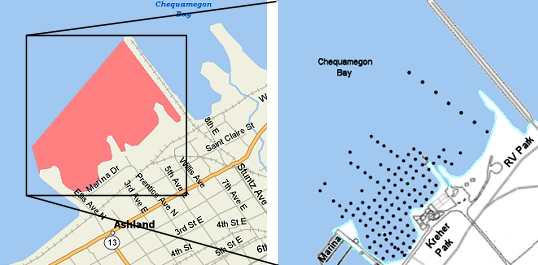
\includegraphics[width=6in]{Figs/Kreher_Park_Map.png}
  \caption{Location of the Ashland superfund site (left) with the location of 119 historical sediment sampling sites (right).}
  \label{fig:KreherParkMap}
\end{figure}

The WDNR wants to study elements in the sediment (among other things) in the entire 3000 m$^2$ area shaded in \figref{fig:KreherParkMap}. Is it physically possible to examine every square meter of that area?  Is it prudent, ecologically and economically, to examine every square meter of this area?  The answer, of course, is ``no.''  How then will the WDNR be able to make conclusions about this entire area if they cannot reasonably examine the whole area?  The most reasonable solution is to sample a subset of the area and use the results from this sample to make inferences about the entire area.

Methods for properly selecting a sample that fairly represents a larger collection of individuals are an important area of study in statistics. For example, the WDNR would not want to sample areas that are only conveniently near shore because this will likely not be an accurate representation of the entire area. In this example, it appears that the WDNR used a grid to assure a relatively even dispersal of samples throughout the study area \figrefp{fig:KreherParkMap}. Methods for choosing the number of individuals to select and how to select those individuals are discussed in \modref{chap:DataProd}.


Suppose that the WDNR measured the concentration of lead at each of the 119 locations shown in \figref{fig:KreherParkMap}. Further suppose that they presented their results at a public meeting by simply showing the list of lead concentration measurements \tabrefp{tab:KreherParkPbconc}.\footnote{These are hypothetical data for this site.}  Is it easy to make conclusions about what these data mean from this type of presentation?

\begin{table}[htbp]   \label{tab:KreherParkPbconc}
  \caption{Lead concentration ($\mu g \cdot m^{-3}$) from 119 sites in Kreher Park superfund site.}
  \begin{center}
% latex table generated in R 3.3.3 by xtable 1.8-2 package
% Wed Apr 26 20:49:42 2017
\begin{tabular}{rrrrrrrrrrrrrrr}
  \hline
  \hline
0.91 & 1.09 & 1.00 & 1.09 & 1.06 & 0.98 & 0.98 & 0.94 & 0.89 & 1.09 & 0.91 & 1.06 & 0.81 & 0.90 & 1.21 \\ 
  1.03 & 0.95 & 1.14 & 0.99 & 0.99 & 0.96 & 1.13 & 0.84 & 1.03 & 0.86 & 0.98 & 1.04 & 0.91 & 1.27 & 0.90 \\ 
  0.87 & 1.23 & 1.12 & 0.98 & 0.79 & 1.10 & 1.06 & 1.09 & 0.73 & 0.81 & 1.18 & 0.92 & 0.82 & 1.11 & 0.97 \\ 
  1.24 & 1.06 & 1.09 & 0.78 & 0.94 & 1.08 & 0.91 & 0.98 & 1.22 & 1.04 & 0.77 & 1.18 & 0.93 & 1.14 & 0.94 \\ 
  1.05 & 0.91 & 1.14 & 0.93 & 0.94 & 0.90 & 1.05 & 1.36 & 1.02 & 0.93 & 1.09 & 1.17 & 0.91 & 1.06 & 0.95 \\ 
  0.88 & 0.67 & 1.12 & 1.06 & 0.99 & 0.89 & 0.83 & 0.99 & 1.33 & 1.00 & 1.05 & 1.11 & 1.01 & 1.25 & 0.96 \\ 
  1.07 & 1.17 & 1.01 & 1.20 & 1.17 & 1.05 & 1.21 & 1.10 & 1.07 & 1.01 & 1.16 & 1.24 & 0.86 & 0.90 & 1.07 \\ 
  1.11 & 0.99 & 0.70 & 0.98 & 1.11 & 1.12 & 1.30 & 1.00 & 0.89 & 0.91 & 0.95 & 1.08 & 1.02 & 0.93 &  \\ 
   \hline
\end{tabular}

  \end{center}
\end{table}

Instead, suppose that the scientists brought a simple plot of the frequency of observed lead concentrations and brief numerical summaries \figrefp{fig:KreherParkPbhist} to the meeting. With these one can easily see that the measurements were fairly symmetric with no obviously ``weird'' values. The lead concentrations ranged from as low as 0.67 $\mu g \cdot m^{-3}$ to as high as 1.36 $\mu g \cdot m^{-3}$ with the measurements centered on approximately 1.0 $\mu g \cdot m^{-3}$. These summaries are discussed in detail in \modref{chap:UnivEDAQuant}. However, at this point, note that summarizing large quantities of data with few graphical or numerical summaries makes it is easier to identify meaning from the data.

\begin{knitrout}
\definecolor{shadecolor}{rgb}{0.922, 0.922, 0.922}\color{fgcolor}\begin{figure}[hbtp]

{\centering 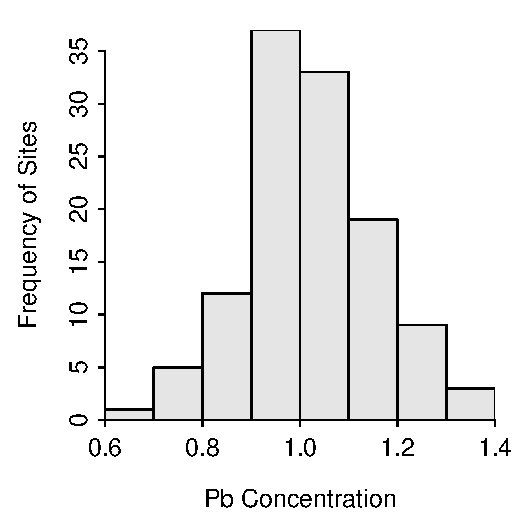
\includegraphics[width=.4\linewidth]{Figs/KreherParkPbhist-1} 
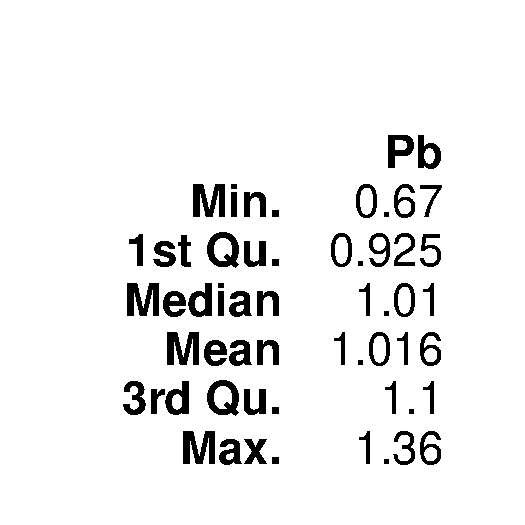
\includegraphics[width=.4\linewidth]{Figs/KreherParkPbhist-2} 

}

\caption[Histogram and summary statistics of lead concentration measurements ($\mu g \cdot m^{-3}$) at each of 119 sites in Kreher Park superfund site]{Histogram and summary statistics of lead concentration measurements ($\mu g \cdot m^{-3}$) at each of 119 sites in Kreher Park superfund site.}\label{fig:KreherParkPbhist}
\end{figure}


\end{knitrout}

A critical question at this point is whether or not the results from the one sample of 119 sites perfectly represents the results for the entire area. One way to consider this question is to examine the results obtained from another sample of 119 sites. The results from this second sample \figrefp{fig:KreherParkPbhist1} are clearly, though not radically, different from the results of the first sample. Thus, it is seen that any one sample from a larger whole will not perfectly represent the large whole. This will lead to some uncertainty in our summaries of the larger whole.

\begin{knitrout}
\definecolor{shadecolor}{rgb}{0.922, 0.922, 0.922}\color{fgcolor}\begin{figure}[hbtp]

{\centering 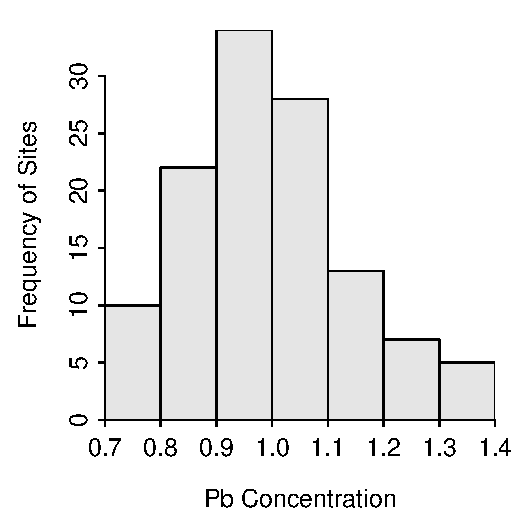
\includegraphics[width=.4\linewidth]{Figs/KreherParkPbhist1-1} 
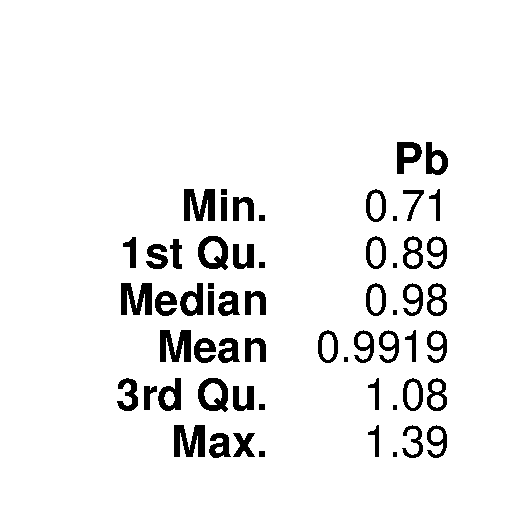
\includegraphics[width=.4\linewidth]{Figs/KreherParkPbhist1-2} 

}

\caption[Kreher Park 1]{Histogram and summary statistics of lead concentration measurements ($\mu g \cdot m^{-3}$) at each of 119 sites (different from the sites shown in \figref{fig:KreherParkPbhist}) in Kreher Park superfund site.}\label{fig:KreherParkPbhist1}
\end{figure}


\end{knitrout}

\vspace{18pt}
The results from two different samples do not perfectly agree because each sample contains different individuals (sites in this example), and no two individuals are exactly alike. The fact that no two individuals are exactly alike is \textbf{natural variability}\index{Natural Variability!Definition}, because of the ``natural'' differences that occur among individuals. The fact that the results from different samples are different is called \textbf{sampling variability}\index{Sampling Variability!Definition}. If there was no natural variability, then there would be no sampling variability. If there was no sampling variability, then the field of statistics would not be needed because a sample (even of one individual) would perfectly represent the larger group of individuals. Thus, understanding variability is at the core of statistical practice. Natural and sampling variability will be revisited continuously throughout this course.

%\defn{Natural Variability}{The fact that no two individuals are exactly alike.}

%\vspace{-12pt}
%\defn{Sampling Variability}{The fact that the results (i.e., statistics) from different samples are different.}

This may be unsettling! First, it was shown that an entire area or all of the individuals of interest cannot be examined. It was then shown that a sample of individuals from the larger whole did not perfectly represent the larger whole. Furthermore, each sample is unique and will likely lead to a (slightly) different conclusion. These are all real and difficult issues faced by the practicing scientist and considered by the informed consumer. However, the field of statistics is designed to ``deal with'' these issues such that the results from a relatively small subset of measurements can be used to make conclusions about the entire collection of measurements.

\warn{Statistics provides methods for overcoming the difficulties caused by the requirement of sampling and the presence of sampling variability.}


\section{Major Goals or Purposes of Statistics}
\vspace{-12pt}
As seen in the Kreher Park example, the field of statistics has two primary purposes. First, statistics provides methods to summarize large quantities of data into concise and informative numerical or graphical summaries. For example, it was easier to discern the general underlying structure of the lead measurements from the statistics and histograms presented in Figures \ref{fig:KreherParkPbhist} and \ref{fig:KreherParkPbhist1}, than it was from the full list of lead measurements in \tabref{tab:KreherParkPbconc}. Second, statistical methods allow inferences to be made about all individuals (i.e., a population) from a few individuals (i.e., a sample).\footnote{Population and sample are defined more completely in \sectref{sect:IVPPSS}.}

%\warn{Statistics, as a field of study, is used to (1) summarize large quantities of data and (2) make inferences about populations from samples.}


\section{Definition of Statistics}
Statistics is the science of collecting, organizing, and interpreting numerical information or data \citep{MooreMcCabe1998}\index{Statistics, Field of!Definition}. People study statistics for a variety of reasons, including \citep{Bluman2000}:
\begin{Enumerate}
  \item To understand the statistical studies performed in their field (i.e., be knowledgeable about the vocabulary, symbols, concepts, and statistical procedures used in those studies).
  \item To conduct research in their field (i.e., be able to design experiments and samples; collect, organize, analyze, and summarize data; make reliable predictions or forecasts for future use; and communicate statistical results).
  \item To be better consumers of statistical information.
\end{Enumerate}

Statistics permeates a wide variety of disciplines. \cite{MooreMcCabe1998} state:
\begin{quote}
The study and collection of data are important in the work of many professions, so that training in the science of statistics is valuable preparation for a variety of careers. Each month, for example, government statistical offices release the latest numerical information on unemployment and inflation. Economists and financial advisers, as well as policy makers in government and business study these data in order to make informed decisions. Doctors must understand the origin and trustworthiness of the data that appear in medical journals if they are to offer their patients the most effective treatments. Politicians rely on data from polls of public opinion. Business decisions are based on market research data that reveal customer tastes. Farmers study data from field trials of new crop varieties. Engineers gather data on the quality and reliability of manufactured products. Most areas of academic study make use of numbers, and therefore also make use of the methods of statistics.
\end{quote}

%\defn{Statistics}{The science of collecting, organizing, and interpreting numerical information or data.}

\begin{exsection}
  \item \label{revex:WhyStatsLakes} There are 1499 lakes in Ashland, Bayfield, and Douglas counties of Wisconsin. However, only 605 of these are named. A random sample of named lakes from this population is extracted with the following R code:
\vspace{-12pt}
\begin{knitrout}
\definecolor{shadecolor}{rgb}{0.922, 0.922, 0.922}\color{fgcolor}\begin{kframe}
\begin{verbatim}
library(NCStats)
named <- filterD(ABDLakes,named)
srsdf(named,n=50,vars=c("county","area"))
\end{verbatim}
\end{kframe}
\end{knitrout}
Use this code and some hand (or calculator) calculations to answer the questions below.
\begin{Enumerate}
  \item Extract a sample of n=50 lakes with the (last line of) code above. Compare the sizes (area in acres) of the first three lakes. This is an example of what type of variability?
  \item Compute the proportion of lakes in your sample that are from Bayfield County.
  \item Extract another sample of n=50 lakes and compute the proportion of lakes that are from Bayfield County? Compare your two proportions. This is an example of what type of variability?
  \item Of the 605 named lakes in the three counties, 346 are from Bayfield County. Was the proportion of named lakes from Bayfield County in either of your samples equal to the proportion of all named lakes that were from Bayfield County?  Were you surprised?  Why or why not?
\end{Enumerate}
\end{exsection}



\chapter{Foundational Definitions} \label{chap:FoundationalDefinitions}
\begin{ChapObj}{\boxwidth}
  \textbf{Objectives:}
  \begin{Enumerate}
    \item Describe what an individual is.
    \item Describe what a population and a sample are and how they differ.
    \item Describe what a parameter and a statistic are and how they differ.
    \item Describe how a population, parameter, sample, and statistic are related.
    \item Identify the individual, variable(s), population, parameter(s), sample, and statistic(s) (IVPPSS) in a given situation.
    \item Identify variable types in context.
  \end{Enumerate}
\end{ChapObj}

\minitoc
\newpage

\lettrine{S}{tatistical inference is the process} of forming conclusions about the unknown parameters of a population by computing statistics from the individuals in a sample.\index{Inference!Definition}  As you can imagine from this definition, it is important that you understand the difference between a population and a sample and a parameter and a statistic before you can understand and appreciate the process of making statistical inferences.  Before identifying these items, the individual and variable(s) of interest must also be identified.  Understanding and identifying these six items is the focus of this module.  Formal methods of inference are discussed beginning with \modref{chap:ProbIntro}.

\defn{Inference}{The process of forming conclusions about the unknown parameters of a population by computing statistics from the individuals in a sample.}

The following hypothetical example is used throughout this module.  Assume that interest is in determining the mean (or average) length of the 1015 fish in Square Lake \figrefp{fig:SquareLakePopn}. In ``real life'' you would not know how many fish are in this lake.  However, for the purpose of illustrating important concepts in this module, it is assumed that all information for all 1015 fish in this lake is known.

\begin{knitrout}
\definecolor{shadecolor}{rgb}{0.922, 0.922, 0.922}\color{fgcolor}\begin{figure}[hbtp]

{\centering 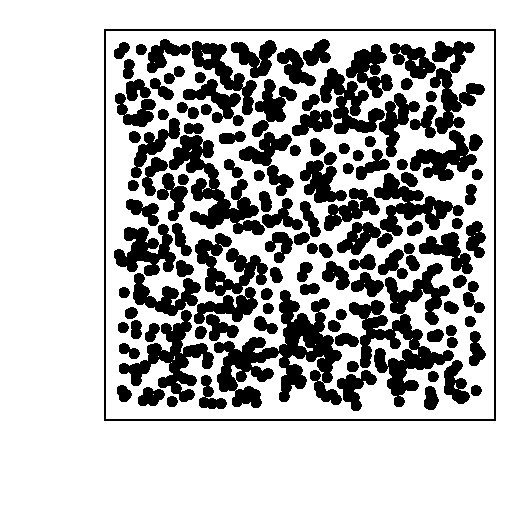
\includegraphics[width=.4\linewidth]{Figs/SquareLakePopn-1} 
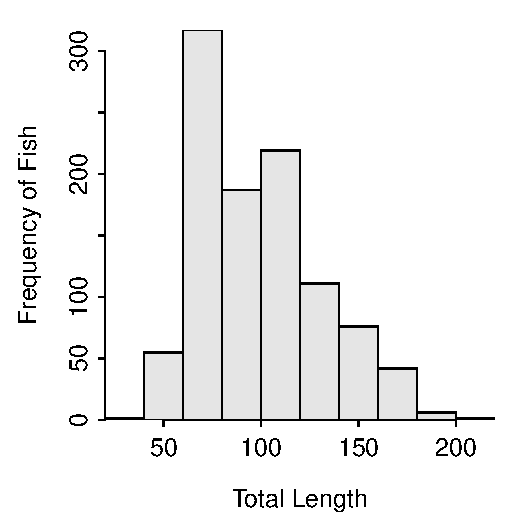
\includegraphics[width=.4\linewidth]{Figs/SquareLakePopn-2} 

}

\caption[Schematic representation of individual fish (i.e., dots]{Schematic representation of individual fish (i.e., dots; \textbf{Left}) and histogram (\textbf{Right}) of the total length of the 1015 fish in Square Lake.}\label{fig:SquareLakePopn}
\end{figure}


\end{knitrout}

\vspace{-24pt}
\section{Definitions} \label{sect:IVPPSS}
\vspace{-12pt}
The \textbf{individual} in a statistical analysis is one of the ``items'' to be examined by the researcher.\index{Individual, Definition}  Sometimes the individual is a person, but it may be an animal, a piece of wood, a site or location, a particular time, or an event.  It is extremely important that you don't always visualize a person when you use the word individual in a statistical context.  Synonyms for individual are unit, experimental unit (usually used in experiments), sampling unit (usually used in observational studies), case, and subject (usually used in studies involving humans).  The individual of interest in the Square Lake example is an individual fish, because the researcher will collect a set of fish and examine each fish individually.

\defn{Individual}{One of the items examined by the researcher.}

\vspace{-12pt}
\warn{An individual is not necessarily a person.}

The \textbf{variable} is the characteristic of interest recorded about each individual.\index{Variable!Definition} The variable of interest in the Square Lake example is the length of each fish. Note that in most ``real life'' studies the researcher will record more than one variable.  For this example, the researcher may also record the fish's weight, sex, and age.  Studies with one variable are called univariate studies, studies with two variables are bivariate studies, and studies with more than two variables are called multivariate studies.

\defn{Variable}{The characteristic of interest recorded about each individual.}

A \textbf{population} is ALL individuals of interest.\index{Population} In the Square Lake example, the population is all 1015 fish in the lake.  The population should be defined as thoroughly as possible including qualifiers as necessary.  This example is simple because Square Lake is so well defined; however, as you will see in the review exercises, the population is often only well-defined by your choice of descriptors.

\defn{Population}{ALL individuals of interest.}

A \textbf{parameter} is a summary computed from ALL individuals in a population.\index{Parameter!Definition}  The term for the particular summary is usually preceded by the word ``population.''  Parameters are ultimately what is of interest because interest is in all individuals in the population.  However, in practice, parameters cannot be computed because the entire population cannot be ``seen.''  In this hypothetical example, the parameters can be computed because all 1015 fish are accessible.  In this example, the researchers were interested in the population mean length of all fish in Square Lake, which is 98.06 mm \tabrefp{tab:SquareLakePopn}.\footnote{We will discuss how to compute and interpret each of these values in later modules.}

% latex table generated in R 3.3.3 by xtable 1.8-2 package
% Wed Apr 26 20:49:43 2017
\begin{table}[ht]
\centering
\caption{Parameters for the total length of ALL 1015 fish in the Square Lake population.} 
\label{tab:SquareLakePopn}
\begin{tabular}{cccccccc}
 n & mean & sd & min & Q1 & median & Q3 & max \\ 
  \hline
1015 & 98.06 & 31.49 & 39 & 72 & 93 & 117 & 203 \\ 
   \hline
\end{tabular}
\end{table}


\defn{Parameter}{A summary of ALL individuals in a population.}

\vspace{-12pt}
\warn{Populations and parameters can generally not be ``seen.''}

The entire population cannot be ``seen'' in real life.  Thus, a subset of the population is usually examined to learn something about the population.  This subset is called a \textbf{sample}.\index{Sample!Definition}  The red dots in \figref{fig:SquareLakeSample1} represent a random sample of n=50 fish from Square Lake (note that the sample size is usually denoted by n).

\begin{knitrout}
\definecolor{shadecolor}{rgb}{0.922, 0.922, 0.922}\color{fgcolor}\begin{figure}[hbtp]

{\centering 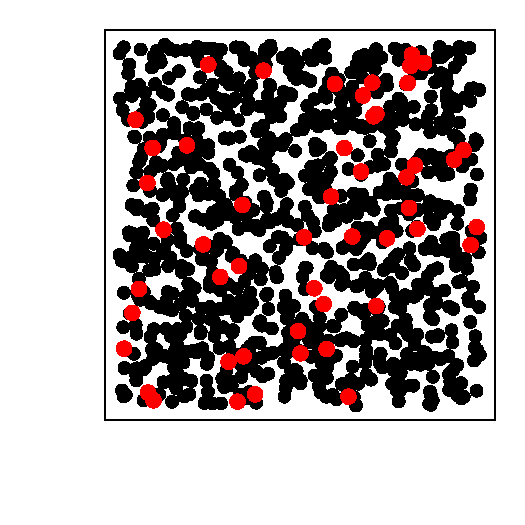
\includegraphics[width=.4\linewidth]{Figs/SquareLakeSample1-1} 
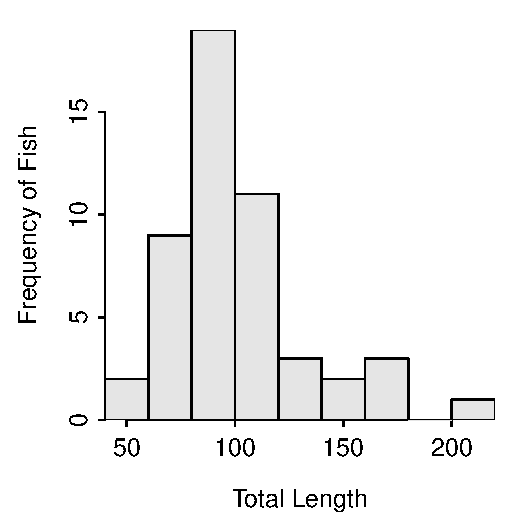
\includegraphics[width=.4\linewidth]{Figs/SquareLakeSample1-2} 

}

\caption{Schematic representation (\textbf{Left}) of a sample of 50 fish (i.e., red dots) from Square Lake and histogram (\textbf{Right}) of the total length of the 50 fish in this sample.}\label{fig:SquareLakeSample1}
\end{figure}


\end{knitrout}

\defn{Sample}{A subset of the population examined by a researcher.}

Summaries computed from individuals in a sample are called \textbf{statistics}.\index{Statistic!Definition}  Specific names of statistics are preceded by ``sample.''  The statistic of interest is always the same as the parameter of interest; i.e., the statistic describes the sample in the same way that the parameter describes the population.  For example, if interest is in the population mean, then the sample mean would be computed.

Some statistics computed from the sample from Square Lake are shown in \tabref{tab:SquareLakeSample1} and \figref{fig:SquareLakeSample1}.  The sample mean of 100.04 mm is the best ``guess'' at the population mean.  Not surprisingly from the discussion in \modref{chap:WhyStatsImportant}, the sample mean does not perfectly equal the population mean.

% latex table generated in R 3.3.3 by xtable 1.8-2 package
% Wed Apr 26 20:49:43 2017
\begin{table}[ht]
\centering
\caption{Summary statistics for the total length of a sample of 50 fish from the Square Lake population.} 
\label{tab:SquareLakeSample1}
\begin{tabular}{cccccccc}
 n & mean & sd & min & Q1 & median & Q3 & max \\ 
  \hline
50 & 100.04 & 31.94 & 49 & 81 & 91 & 118 & 203 \\ 
   \hline
\end{tabular}
\end{table}


\defn{Statistic}{A summary of all individuals in a sample.}


\section{Performing an IVPPSS}
\vspace{-12pt}
In each statistical analysis it is important that you determine the Individual, Variable, Population, Parameter, Sample, and Statistic (\textbf{IVPPSS}). First, determine what items you are actually going to look at; those are your individuals.  Second, what are you going to record when you look at an individual; that is the variable.  Third, the population is simply ALL of the individuals.  Fourth, the parameter is a summary (e.g., mean or proportion) of the variable recorded from ALL of the individuals in the population.\footnote{Again, parameters generally cannot be computed because all of the individuals in the population can not be seen.  Thus, the parameter is largely conceptual.}  Fifth, we usually cannot see all of the individuals in the population so only a few are examined; those few are the sample.  Finally, the summary of the individuals in the sample is the statistic.

When performing an IVPPSS, keep in mind that parameters describe populations (note that they both start with ``p'') and statistics describe samples (note that they both start with ``s'').  This can also be looked at from another perspective.  A sample is an estimate of the population and a statistic is an estimate of a parameter.  Thus, the statistic has to be the same summary (mean or proportion) of the sample as the parameter is of the population.

The IVPPSS process is illustrated for the following situation:
\vspace{-12pt}
\begin{quote}
\textit{A University of New Hampshire graduate student (and Northland College alum) investigated habitat utilization by New England (Sylvilagus transitionalis) and Eastern (Sylvilagus floridanus) cottontail rabbits in eastern Maine in 2007.  In a preliminary portion of his research he determined the proportion of ``rabbit patches'' that were inhabited by New England cottontails.  He examined 70 ``patches'' and found that 53 showed evidence of inhabitance by New England cottontails.}
\end{quote}

\begin{Itemize}
  \item An individual is a rabbit patch in eastern Maine in 2007 (i.e., a rabbit patch is the ``item'' being sampled and examined).
  \item The variable is ``evidence for New England cottontails or not (yes or no)'' (i.e., the characteristic of each rabbit patch that was recorded).
  \item The population is ALL rabbit patches in eastern Maine in 2007.
  \item The parameter is the proportion of ALL rabbit patches in eastern Maine in 2007 that showed evidence for New England cottontails.\footnote{Note that this population and parameter cannot actually be calculated but it is what the researcher wants to know.}
  \item The sample is the 70 rabbit patches from eastern Maine in 2007 that were actually examined by the researcher.
  \item The statistic is the proportion of the 70 rabbit patches from eastern Maine in 2007 actually examined that showed evidence for New England cottontails. [In this case, the statistic would be 53/70 or 0.757.]
\end{Itemize}

In some situations it may be easier to identifying the sample first.  From this, and through the realization that a sample is always ``of the individuals'', it may be easier to identify the individual.  This process is illustrated in the following example, with the items listed in the order identified rather than in the traditional IVPPSS order.

\begin{quote}
\textit{The Duluth, MN Touristry Board is interested in the average number of raptors seen per year at Hawk Ridge.\footnote{Information about Hawk Ridge is found \href{http://www.hawkridge.org/}{here}.}  To determine this value, they collected the total number of raptors seen in a sample of years from 1971-2003.}
\end{quote}

\begin{Itemize}
  \item The sample is the 32 years between 1971-2003 at Hawk Ridge.
  \item An individual is a year (because a ``sample of \emph{years}'' was taken) at Hawk Ridge.
  \item The variable recorded was the number of raptors seen in one year at Hawk Ridge.
  \item The population is ALL years at Hawk Ridge(this is a bit ambiguous but may be thought of as all years that Hawk Ridge has existed).
  \item The parameter is the average number of raptors seen per year in ALL years at Hawk Ridge.
  \item The statistic is the average number of raptors seen in the 1971-2003 sample of years at Hawk Ridge.
\end{Itemize}

\begin{exsection}
  \item \label{revex:IVPPSSDad}My Dad owns 60 acres of timber (mostly Oak, Walnut, and Poplar) in Iowa.  He wants to measure the mean diameter-at-breast-height (DBH) of the oak trees on his property.  He measures the DBH of 75 randomly selected oak trees.  Use this information to perform an IVPPSS. \ansref{ans:IVPPSSDad}
  \item \label{revex:IVPPSSFishStore}I have a friend who wants to start a (fishing) bait store on the West end of Ashland.  He wants to determine what proportion of Ashland residents who currently use the East end bait store would use a store in the West end if one existed.  He sends out 5000 questionnaires and receives 2378 back from patrons of the East end store.   Use this information to perform an IVPPSS.  \ansref{ans:IVPPSSFishStore}
  \item \label{revex:IVPPSSNBA}I'm interested in developing a model to predict how many points an NBA starting basketball player scores. Therefore, I want to determine the relationship between points scored and height, speed (in the 40-yard dash), position, and minutes played. To identify this relationship I gather these data from 100 NBA starting basketball players.  Use this information to perform an IVPPSS. \ansref{ans:IVPPSSNBA}
  \item \label{revex:IVPPSSClinton}Pollsters wanted to determine the proportion of registered voters who approved of President Clinton's performance.  They called 5000 randomly selected registered voters and ask 4123 of those (the rest weren't home, didn't answer, or hung up) ``Do you approve of Pres. Clinton's performance?''  Use this information to perform an IVPPSS. \ansref{ans:IVPPSSClinton}
  \item \label{revex:IVPPSSGoslings}You Might Be Interested To Know (YMBITK), the average level of mercury in newly-hatched goslings in the upper Midwest (MI, MN, ND, SD, WI). You obtained 20 goslings from resource agencies in each state.  Use this information to perform an IVPPSS. \ansref{ans:IVPPSSGoslings}
  \item \label{revex:IVPPSSNClead}YMBITK, the proportion of NC students that think NC can become ``the nation's leading environmental liberal arts college'' in the next decade. You polled 124 students.  Use this information to perform an IVPPSS. \ansref{ans:IVPPSSNClead}
  \item \label{revex:IVPPSSStudy}YMBITK, the relationship between hours studied and GPA of students in the UW system (excluding UW-Madison). You interviewed 250 students from throughout the system.  Use this information to perform an IVPPSS. \ansref{ans:IVPPSSStudy}
  \item \label{revex:IVPPSSCoach}YMBITK, the average difference in salaries between the head coaches of men's and head coaches of women's basketball teams at Division I schools. You interviewed 73 head-coach pairs.  Use this information to perform an IVPPSS. \ansref{ans:IVPPSSCoach}
  \item \label{revex:IVPPSSBioGrads}YMBITK, the proportion of graduates from small private schools, who majored in Biology and who have been out of school for at least 5 years, that feel that statistics is an ``important'' course. You interviewed 1023 people.  Use this information to perform an IVPPSS. \ansref{ans:IVPPSSBioGrads}
  \item \label{revex:IVPPSSBaikal}Scientist in Chivyrkui Bay on Lake Baikal \citep{OwensPronin2000} were interested, among other things, in determining the mean age of pike (\textit{Esox lucius}) in the bay. They collected scales from 30 fish using gill nets and angling methods. Use this information to perform an IVPPSS. \ansref{ans:IVPPSSBaikal}
  \item \label{revex:IVPPSSRuffe}The Eurasian ruffe is an exotic species of fish that is causing some alarm in fisheries biologists in the Great Lakes area \citep{Maniaketal2000}. A few of these biologists tested to see if a certain pheromone released by injured ruffe would repel other ruffe.  If so, natural, or possibly synthetic, versions of this pheromone could be used to distract ruffe from areas in which they are causing damage. In their experiment, they observed ruffe held in aquaria divided into four sections.  They recorded what proportion of 24 randomly-selected ruffe caught in the St. Louis River Harbor, and then held in the aquaria, left a section when the chemical was added to that section.  Use this information to perform an IVPPSS. \ansref{ans:IVPPSSRuffe}
\end{exsection}


\subsection{Sampling Variability (Revisited)}
It is instructive to once again (see \modref{chap:WhyStatsImportant}) consider how statistics differ among samples.  \tabref{tab:SquareLakeSample234} and \figref{fig:SquareLakeSample234} show results from three more samples of n=50 fish from the Square Lake population.  The means from all four samples (including the sample in \tabref{tab:SquareLakeSample1} and \figref{fig:SquareLakeSample1}) were quite different from the known population mean of 98.06 mm.  Similarly, all four histograms were similar in appearance but were slightly different in actual values. These results illustrate that a statistic (or sample) will only approximate the parameter (or population) and that statistics vary among samples.  This \textbf{sampling variability} is one of the most important concepts in statistics and will be discussed in great detail beginning in \modref{chap:SamplingDist}.\index{Sampling Variability!Definition}

\begin{knitrout}
\definecolor{shadecolor}{rgb}{0.922, 0.922, 0.922}\color{fgcolor}\begin{figure}[hbtp]

{\centering 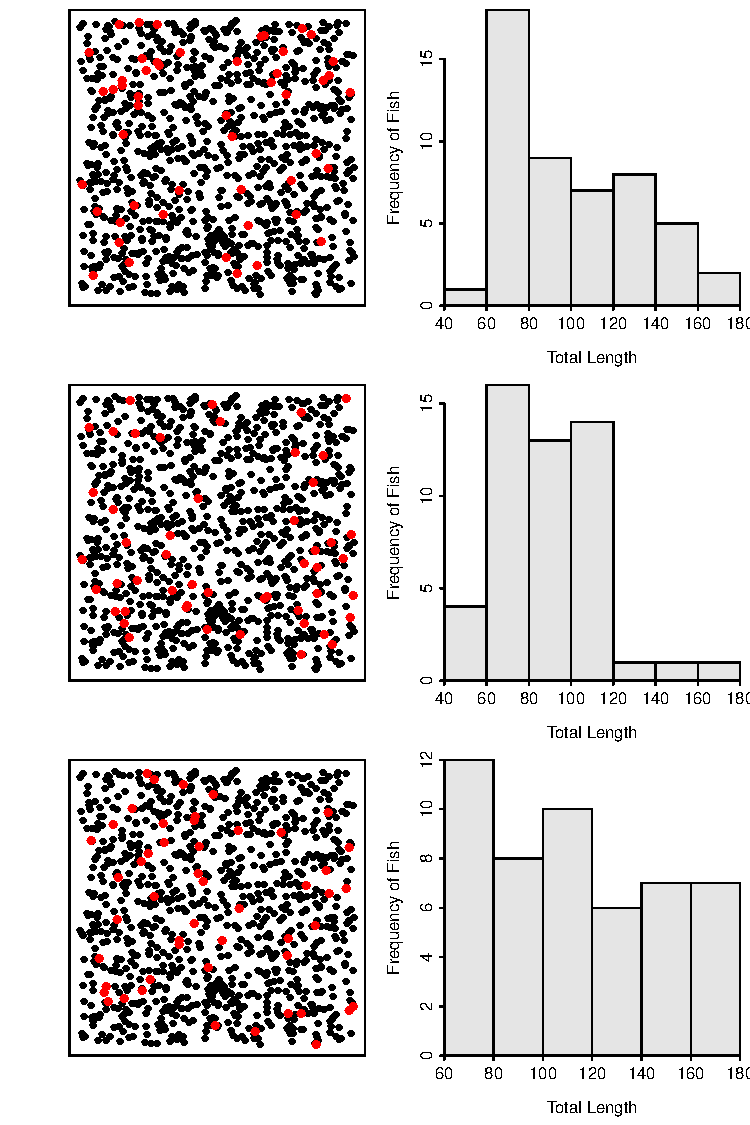
\includegraphics[width=.7\linewidth]{Figs/SquareLakeSample234-1} 

}

\caption{Schematic representation (\textbf{Left}) of three samples of 50 fish (i.e., red dots) from Square Lake and histograms (\textbf{Right}) of the total length of the 50 fish in each sample.}\label{fig:SquareLakeSample234}
\end{figure}


\end{knitrout}

% latex table generated in R 3.3.3 by xtable 1.8-2 package
% Wed Apr 26 20:49:43 2017
\begin{table}[htbp]
\centering
\caption{Summary statistics for the total length in three samples of 50 fish from the Square Lake population.} 
\label{tab:SquareLakeSample234}
\begin{tabular}{cccccccc}
 n & mean & sd & min & Q1 & median & Q3 & max \\ 
  \hline
50 & 99.56 & 32.47 & 57 & 69 & 91 & 123 & 167 \\ 
  50 & 88.64 & 24.52 & 53 & 68 & 86 & 106 & 166 \\ 
  50 & 112.74 & 35.86 & 61 & 84 & 108 & 147 & 174 \\ 
   \hline
\end{tabular}
\end{table}


\defn{Sampling Variability}{The realization that no two samples are exactly alike. Thus, statistics computed from different samples will likely vary.}

This example also illustrates that parameters are fixed values because populations don't change.  If a population does change, then it is considered to be a different population.  In the Square Lake example, if a fish is removed from the lake, then the lake would then be considered a different population of fish.  Statistics, on the other hand, vary depending on the sample because each sample consists of different individuals that vary (i.e., sampling variability exists because natural variability exists).

\warn{Parameters are fixed in value, while statistics vary in value.}


\clearpage
\section{Variable Types}\label{sect:VarTypes}
The type of statistic that can be calculated is dictated by the type of variable to be analyzed.  For example, a sample mean (or average) can only be calculated for a quantitative variable (defined below).  Thus, the type of that variable should be identifie immediately after performing an IVPPSS.

\subsection{Variable Definitions}
There are two main groups of variable types -- quantitative and categorical \figrefp{fig:VarTypes}.  \textbf{Quantitative} variables are variables with numerical values for which it makes sense to do arithmetic operations (like adding or averaging).\index{Quantitative Variable}  Synonyms for quantitative are measurement or numerical.  \textbf{Categorical} variables are variables that record to which group or category an individual belongs.\index{Categorical Variable}  Synonyms for categorical are qualitative or attribute.  Within each main type of variable are two subgroups \figrefp{fig:VarTypes}.

\begin{knitrout}
\definecolor{shadecolor}{rgb}{0.922, 0.922, 0.922}\color{fgcolor}\begin{figure}[hbtp]

{\centering 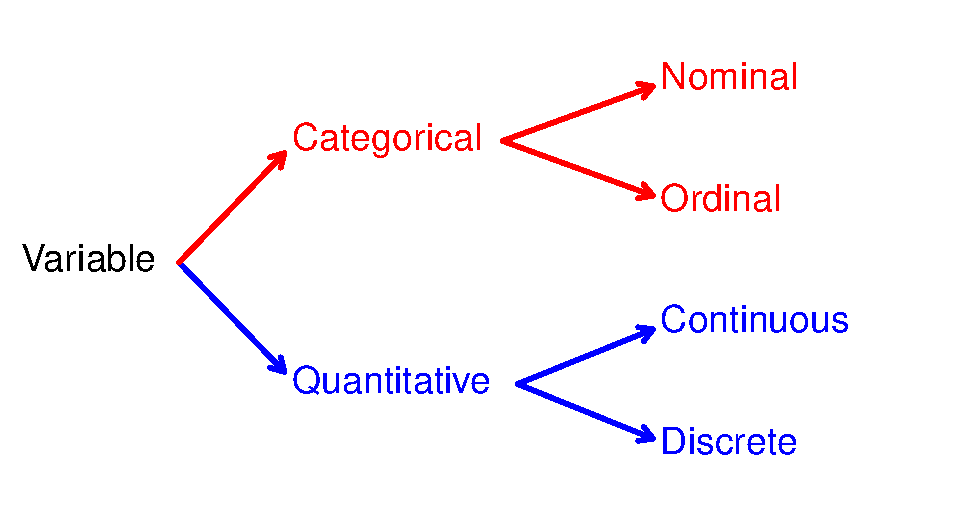
\includegraphics[width=.5\linewidth]{Figs/VarTypes-1} 

}

\caption[Schematic representation of the four types of variables]{Schematic representation of the four types of variables.}\label{fig:VarTypes}
\end{figure}


\end{knitrout}
\vspace{9pt} % added because of paragraph compressions following R code

The two types of quantitative variables are continuous and discrete variables.  \textbf{Continuous} variables are quantitative variables that have an uncountable number of values.\index{Continuous Variable}  In other words, a potential value \textsc{does} exist between every pair of values of a continuous variable.  \textbf{Discrete} variables are quantitative variables that have a countable number of values.\index{Discrete Variable}  Stated differently, a potential value \textsc{does not} exist between every pair of values of a discrete variable.  Typically, but not always, discrete variables are counts of items.

Continuous and discrete variables are easily distinguished by determining if it is possible for a value to exist between every two values of the variable.  For example, can there be between 2 and 3 ducks on a pond?  No!  Thus, the number of ducks is a discrete variable.  Alternatively, can a duck weigh between 2 and 3 kg?  Yes!  Can it weigh between 2 and 2.1 kg?  Yes!  Can it weigh between 2 and 2.01 kg?  Yes!  You can see that this line of questions could continue forever; thus, duck weight is a continuous variable.

\defn{Discrete Variable}{A quantitative variable that can assume a countable number of values.}

\vspace{-12pt}
\defn{Continuous Variable}{A quantitative variable that can assume an uncountable number of values.}

\vspace{-12pt}
\warn{A quantitative variable is continuous if a possible value exists between every two values of the variable; otherwise, it is discrete.}

The two types of categorical variables are ordinal and nominal.  \textbf{Ordinal} variables are categorical variables where a natural order or ranking exists among the categories.\index{Ordinal Variable}  \textbf{Nominal} variables are categorical variables where no order or ranking exists among the categories.\index{Nominal Variable}

Ordinal and nominal variables are easily distinguished by determining if the order of the categories matters.  For example, suppose that a researcher recorded a subjective measure of condition (i.e., poor, average, excellent) and the species of each duck.  Order matters with the condition variable -- i.e., condition improves from the first (poor) to the last category (excellent) -- and some reorderings of the categories would not make sense -- i.e., average, poor, excellent does not make sense.  Thus, condition is an ordinal variable.  In contrast, species (e.g., mallard, redhead, canvasback, and wood duck) is a nominal variable because there is no inherent order among the categories (i.e., any reordering of the categories also ``makes sense'').

\defn{Ordinal Variable}{A categorical variable for which a natural order exists among the categories.}

\vspace{-12pt}
\defn{Nominal Variable}{A categorical variable for which a natural order DOES NOT exist among the categories.}

\vspace{-12pt}
\warn{Remember that \textbf{ord}inal means that an \textbf{ord}er among the categories exists (note ``ord'' in both ordinal and order).}

The following are some issues to consider when identifying the type of a variable:
\begin{Enumerate}
  \item The categories of a categorical variable are sometimes labeled with numbers. For example, 1=``Poor'', 3=``Fair'', and 5=``Good''.  Don't let this fool you into calling the variable quantitative.
  \item Rankings, ratings, and preferences are ordinal (categorical) variables.
  \item Counts of numbers are discrete (quantitative) variables.
  \item Measurements are typically continuous (quantitative) variables.
  \item It does not matter how precisely quantiative variables are recorded when deciding if the variable is continuous or discrete. For example, the weight of the duck might have been recorded to the nearest kg. However, this was just a choice that was made, the actual values can be continuously finer than kg and, thus, weight is a continuous variable.
  \item Categorical variables that consist of only two levels or categories will be labeled as a nominal variable (because any order of the groups makes sense).  This type of variable is also often called ``binomial.''.
  \item Do not confuse ``what type of variable'' (answer is one of ``continuous'', ``discrete'', ``nominal'', or ``ordinal'')  with ``what type of variability'' (answer is ``natural'' or ``sampling'') questions.
\end{Enumerate}

\warn{``What type of variable is ...?'' is a different question than ``what type of variability is ...?''  Be careful to note the word difference (i.e., ``variable'' versus ``variability'' when answering these questions.}

\vspace{-12pt}
\warn{The precision to which a quantitative variable was recorded does not determine whether it is continuous or discrete. How precisely the variable COULD have been recorded is the important consideration.}

\begin{exsection}
  \item \label{revex:VarTypeDucks} What type of variable is the number of ducks found at the ``Hot Pond'' every morning? \ansref{ans:VarTypeDucks}
  \item \label{revex:VarTypeGenetics} What type of variable is the genotype (AA, Aa, aa) of a particular species of sunflower? \ansref{ans:VarTypeGenetics}
  \item \label{revex:VarTypeGenetics2} What type of variable is the length of petals on individual flowers? \ansref{ans:VarTypeGenetics2}
  \item \label{revex:VarTypeGenetics3} What type of variable is the number of seeds produced by an individual sunflower? \ansref{ans:VarTypeGenetics3}
  \item \label{revex:VarTypeGenetics4} What type of variable is the ``quality'' of the seeds produced by an individual plant (``quality'' is recorded as 1=poor, 2=low, 3=good, and 4=excellent)? \ansref{ans:VarTypeGenetics4}
  \item \label{revex:VarTypeSOS} What type of variable is student rankings (``Excellent'', ``Very Good'', ``Good'', ``Fair'', ``Poor'') of a professor's abilities? \ansref{ans:VarTypeSOS}
  \item \label{revex:VarTypeAudit} What type of variable is whether an account is valid or invalid? \ansref{ans:VarTypeAudit}
  \item \label{revex:VarTypeDefects} What type of variable is the number of defects produced by a machine? \ansref{ans:VarTypeDefects}
  \item \label{revex:VarTypeBottles} What type of variable is the ounces of cola in a sample of 100 bottles? \ansref{ans:VarTypeBottles}
  \item \label{revex:VarTypeFish} What type of variable is the sex of fish collected from a lake? \ansref{ans:VarTypeFish}
  \item \label{revex:VarTypeFrogs} What type of variable is the number of legs on frogs collected in Bayfield County? \ansref{ans:VarTypeFrogs}
  \item \label{revex:VarTypeCroak} What type of variable is the frequency (mhz) of a bullfrog's ``croak''? \ansref{ans:VarTypeCroak}
  \item \label{revex:VarTypeTowns} What type of variable is the number of incorporated towns in a county? \ansref{ans:VarTypeTowns}
  \item \label{revex:VarTypeWeasels} What type of variable is the qualitative size of least weasels (small, medium, large)? \ansref{ans:VarTypeWeasels}
\end{exsection}



\chapter{Data Production} \label{chap:DataProd}
\begin{ChapObj}{\boxwidth}
  \textbf{Objectives:}
  \begin{Enumerate}
    \item Identify major differences between data produced from experiments and observational studies.
    \item Understand basic ideas of simple random experiments with one and two factors.
    \item Describe the principles of experimental design.
    \item Describe the principles of observational studies.
    \item Understand basic ideas of designing simple observational studies, and
    \item Explain the importance of randomization in both experiments and observational studies.
  \end{Enumerate}
\end{ChapObj}

\minitoc
\newpage

\lettrine{S}{tatistical inference is the process} of making conclusions about an entire population based on the results from the individuals in a single sample.\index{Inference!Definition}  To make conclusions about the larger population from a sample requires a sample that fairly represents the larger population.  In this module, two ways of producing data -- (1) Experiments and (2) Observational Studies -- are described.  The proper collection (or production) of data is critical to statistics (and science in general) so that proper inferences and conclusions can be made.

\defn{Inference}{The process of forming conclusions about the unknown parameters of a population by computing statistics from the individuals in a sample.}

\warn{If data are not properly collected, then inferences cannot be made.}


\section{Experiments}
An experiment deliberately imposes a condition, or treatment, on individuals to observe their response.\index{Experiment!Definition}  In a properly designed experiment all variables that are not of interest are held constant while the variable(s) that are of interest are changed among treatments.  As long as the experiment is designed properly (see below), tests for differences in the response variable among treatments can be made.  If differences among treatments occur, then those differences are due either to the variable(s) that were deliberately changed or randomness (chance).  Thus, strong cause-and-effect statements can be made from data collected with a carefully designed experiment.

\warn{An experiment deliberately imposes a condition, or treatment, on individuals in order to observe their response.}

\vspace{-12pt}
\warn{Strong cause-and-effect statements can be made from data collected with a carefully designed experiment.}

\subsection{Single-factor Experiments}\index{Experiment!Single-Factor}
A factor is the variable that is deliberately manipulated to determine its effect on the response variable.\index{Factor!Experiment}  Sometimes the factor is called an explanatory variable because we are attempting to determine how it affects (or ``explains'') the response variable.\index{Response Variable!Experiment}  The simplest experiment is a single-factor experiment where the individuals are split into groups defined by the categories of a single factor variable.

For example, suppose that a research group wants to examine the effect of temperature on the total number of bacterial cells after two weeks. They have inoculated 120 agars (petri dishes with a growth medium for the bacteria) with the bacteria and placed them in a chamber where all environmental conditions (e.g., temperature, humidity, light) can be controlled exactly.  The researchers will use only two temperatures in this simple experiment -- $10^{o}$C and $15^{o}$C.  Thus, temperature is the only factor in this simple experiement because it is the only variable manipulated to different values to determine its impact on the number of bacterial cells.

\defn{Factor(s)}{The variable(s) that is (are) deliberately manipulated in the experiment to determine its effect on the response variable.  Sometimes called the explanatory variable.}

\vspace{-12pt}
\defn{Response}{The variable observed in an experiment to identify the effect of the factors on it.}

\vspace{-12pt}
\warn{In a single-factor experiment only one explanatory variable (i.e., factor) is allowed to vary; all other explanatory variables are held constant.}

Levels are the number of categories of the factor variable.\index{Level!Experimental}  In this example, there are two levels -- $10^{o}$C and $15^{o}$C.  Treatments are the number of unique conditions that individuals in the experiment are exposed to.  In a single-factor experiment, the number of treatments is the same as the number of levels of the factor.\index{Treatment, Experimental}  Thus, in this simple experiment, there are two treatments -- $10^{o}$C and $15^{o}$C.  Treatments are discussed more thoroughly in the next section.

The number of replicates in an experiment is the number of individuals that will receive each treatment.\index{Replicates}  In this example, the replicates are the number of inoculated agars that will receive each of the two temperature treatments.  The number of replicates is determined by dividing the total number of available individuals (120) by the number of treatments (2).  In this case, the number of replicates is 60 inoculated agars.

\defn{Levels}{The number of categories or groupings of the factor.}

\vspace{-12pt}
\warn{In single-factor experiments, the number of treatments in the experiment equals the number of levels of the single factor.}

\vspace{-12pt}
\defn{Replicates}{The number of individuals in each treatment group.}

\vspace{-12pt}
\warn{The number of replicates is determined by dividing the total number of available individuals by the number of treatments.}

The agars used in this experiment will be randomly allocated to the two temperature treatments.  All other variables -- humidity, light, etc. -- are kept the same for each treatment.  At the end of two weeks, the total number of bacterial cells on each agar (i.e., the response variable) will be recorded and compared between the agars kept at both temperatures.\footnote{Methods for making this comparison are in \modref{chap:tTest2}.}  Any difference in mean number of bacterial cells will be due to either different temperature treatments or randomness, because all other variables were the same between the two treatments.

\warn{Differences among treatments are either caused by randomness (chance) or the factor.}

The single factor is not restricted to just two levels.  For example, more than two temperatures, say $10^{o}$C, $12.5^{o}$C, $15^{o}$C, and $17.5^{o}$C, could have been tested.  With this modification, there is still only one factor -- temperature -- but there are now four levels (and only four treatments).

\subsection{Multi-factor Experiments}
More than one factor can be tested in one experiment.\index{Experiment!Multi-Factor}  In fact, it is more efficient to have a properly designed experiment where more than one factor is varied at a time than it is to use separate experiments in which only one factor is varied in each.  However, before showing this benefit, let's examine the definitions from the previous section in a multi-factor experiment.

Suppose that the previous experiment was modified to also examine the effect of relative humidity on the number of bacteria cells.  This modified experiment has two factors -- temperature (with two levels of $10^{o}$C or $15^{o}$C) and relative humidity (with four levels of 20\%, 40\%, 60\%, and 80\%).  The number of treatments, or combinations of all factors, in this experiment is found by multiplying the levels of all factors (i.e., 2$\times$4=8 in this case).\index{Treatment, Experimental}  The number of replicates in this experiment is now 15 (i.e., total number of available agars divided by eight; 120/8).

A quick drawing of the experimental design can be instructive (below).  The drawing is a grid where the levels of one factor are the rows and the levels of the other factor are the columns.  The number of rows and columns correspond to the levels of the two factors, respectively, whereas the number of cells in the grid is the number of treatments (numbered in this table to show eight treatments).

\begin{center}
\begin{tabular}{cc|c|c|c}
 & \multicolumn{4}{c}{Relative Humidity} \\
\cline{2-5}
 & 20\% & 40\% & 60\% & 80\% \\
\cline{2-5}
\multicolumn{1}{c|}{$10^{o}$C} & 1 & 2 & 3 & \multicolumn{1}{c|}{4} \\
\hline
\multicolumn{1}{c|}{$15^{o}$C} & 5 & 6 & 7 & \multicolumn{1}{c|}{8} \\
\cline{2-5}
\end{tabular}
\end{center}

\defn{Treatments}{The number of combinations of all factors in the experiment.}

\vspace{-12pt}
\warn{The number of treatments equals the product of the levels for each factor.}

\vspace{-12pt}
\warn{The number of treatments is determined for the overall experiment, whereas the number of levels is determined for each factor.}

The analysis of a multi-factor experimental design is more involved than what will be shown in this course.  However, multi-factor experiments have many benefits, which can be illustrated by comparing a multi-factor experiment to separate single-factor experiments.  Let's continue with the experiment to identify the effect of both temperature and relative humidity on the number of bacterial cells.  However, consider for the moment that (1) separate single-factor experiments will also be conducted to determine the effect of each factor and (2) we cannot use any of the individuals (i.e., agars) in more than one experiment.

To conduct the two separate experiments, randomly split the 120 available agars into two equally-sized groups of 60.  The first 60 will be split into two groups of 30 for the first experiment with temperature.  The second 60 will be split into four groups of 15 for the second experiment with relative humidity. These separate single-factor experiments are summarized in the following tables (where the numbers in the cells represent the number of replicates in each treatment).

\begin{center}
\begin{tabular}{|c|c|c|c|c|c|c|}
\multicolumn{2}{c}{Temperature} & \multicolumn{1}{c}{} & \multicolumn{4}{c}{Relative Humidity} \\
\cline{1-2}\cline{4-7}
$10^{o}$C & $15^{o}$C & & 20\% & 40\% & 60\% & 80\% \\
\cline{1-2}\cline{4-7}
30 & 30 & & 15 & 15 & 15 & 15 \\
\cline{1-2}\cline{4-7}
\end{tabular}
\end{center}

Now reconsider the design where both factors were varied at once (the table below was modified to include the number of replicates in each treatment).

\begin{center}
\begin{tabular}{cc|c|c|c}
 & \multicolumn{4}{c}{Relative Humidity} \\
\cline{2-5}
 & 20\% & 40\% & 60\% & 80\% \\
\cline{2-5}
\multicolumn{1}{c|}{$10^{o}$C} & 15 & 15 & 15 & \multicolumn{1}{c|}{15} \\
\hline
\multicolumn{1}{c|}{$15^{o}$C} & 15 & 15 & 15 & \multicolumn{1}{c|}{15} \\
\cline{2-5}
\end{tabular}
\end{center}

The key to examining the benefits of the multi-factor experiment is to determine the number of individuals that give ``information'' about (i.e., are exposed to) each factor.  From the last table it is seen that all 120 individuals are exposed to one of the temperature levels with 60 individuals exposed to each level.  In contrast, only 30 individuals were exposed to these levels in the single-factor experiment.  In addition, all 120 individuals are exposed to one of the relative humidity levels with 30 individuals exposed to each level.  Again, this is in contrast to the single-factor experiment where only 15 individuals were exposed to these levels.  Thus, the first advantage of multi-factor experiments is that the available individuals are used more efficiently.  In other words, more ``information'' (i.e., the responses of more individuals) is obtained from a multi-factor experiment than from combinations of single-factor experiments.\footnote{The real importance of this advantage will become apparent when statistical power is introduced in \modref{chap:HypothesisTests}.}

\warn{Multi-factor experiments use individuals more efficiently; i.e., more ``information'' about the effect of the factors on the response is gained from the same number of individuals.}

A properly designed multi-factor experiment also allows researchers to determine if multiple factors interact to impact an individual's response.\index{Interaction effect}  For example, consider the hypothetical results from this experiment in \figref{fig:ExpDInt}.\footnote{The means of each treatment are plotted and connected with lines in this plot.}  The effect of relative humidity is to increase the growth rate for those individuals at $10^{o}$C (black line) but to decrease the growth rate for those individuals at $15^{o}$C (blue line).  That is, the effect of relative humidity differs depending on the level of temperature.  When the effect of one factor differs depending on the level of the other factor, then the two factors are said to \textit{interact}.  Interactions cannot be determined from the two single-factor experiments because the same individuals are not exposed to levels of the two factors at the same time.

\begin{knitrout}
\definecolor{shadecolor}{rgb}{0.922, 0.922, 0.922}\color{fgcolor}\begin{figure}[hbtp]

{\centering 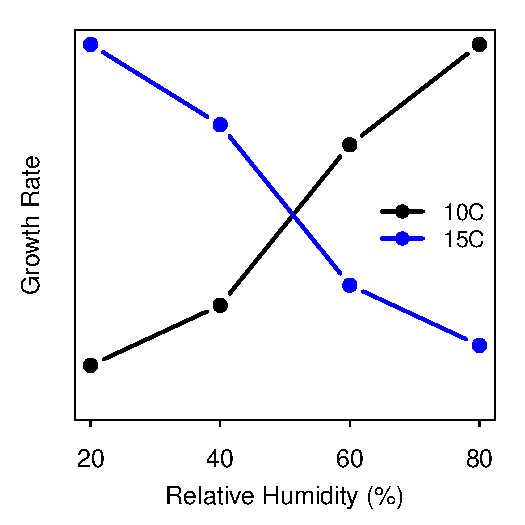
\includegraphics[width=.4\linewidth]{Figs/ExpDInt-1} 

}

\caption[Mean growth rates in a two-factor experiment that depict an interaction effect]{Mean growth rates in a two-factor experiment that depict an interaction effect.}\label{fig:ExpDInt}
\end{figure}


\end{knitrout}
\vspace{9pt} % added because of paragraph compressions following R code

Multi-factor experiments are used to detect the presence or absence of interaction, not just the presence of it.  The hypothetical results in \figref{fig:ExpDNoInt} show that the growth rate increases with increasing relative humidity at about the same rate for both temperatures.  Thus, because the effect of relative humidity is the same for each temperature (and vice versa), there does not appear to be an interaction between the two factors.  Again, this could not be determined from the separate single-factor experiments.

\begin{knitrout}
\definecolor{shadecolor}{rgb}{0.922, 0.922, 0.922}\color{fgcolor}\begin{figure}[hbtp]

{\centering 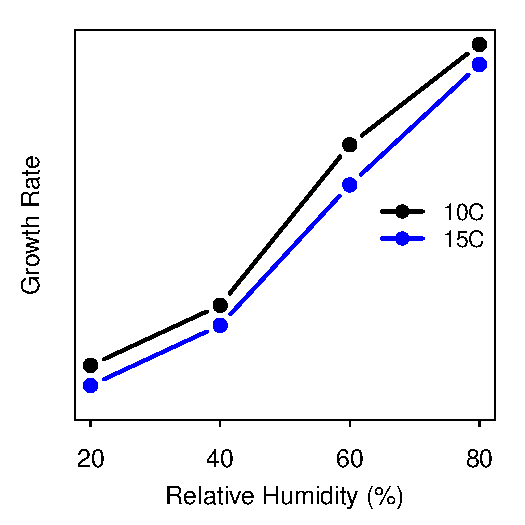
\includegraphics[width=.4\linewidth]{Figs/ExpDNoInt-1} 

}

\caption[Mean growth rates in a two-factor experiment that depict no interaction effect]{Mean growth rates in a two-factor experiment that depict no interaction effect.}\label{fig:ExpDNoInt}
\end{figure}


\end{knitrout}

\warn{Multi-factor experiments can be used to detect interactions between multiple factors.}


\subsection{Allocating Individuals}
In the previous examples, each individual\footnote{When discussing experiments, an ``individual'' is often referred to as a ``replicate'' or an ``experimental unit.''} was allocated to (i.e., placed into) treatments.\index{Replicates}  Individuals should be randomly allocated to treatments.  Randomization will tend to even out differences among groups for variables not considered in the experiment.  In other words, randomization should help assure that all groups are similar before the treatments are imposed.  Thus, randomly allocating individuals to treatments removes any bias (foreseen or unforeseen) from entering the experiment.

In the single-factor experiment above -- two treatments of temperature -- there were 120 agars.  To randomly allocate these individuals to the treatments, 60 pieces of paper marked with ``10'' and 60 marked with ``15'' could be placed into a hat.  One piece of paper would be drawn for each agar and the agar would receive the temperature found on the piece of paper.  Alternatively, each agar could be assigned a unique number between 1 and 120 and pieces of paper with these numbers could be placed into the hat.  The agars corresponding to the first 60 numbers drawn from the hat could then be placed into the first treatment with the agars for the next (or remaining) 60 numbers in the second treatment.  This process is essentially the same as randomly ordering the 120 numbers.  A random order of numbers is obtained with R by including the count of numbers as the only argument to \R{sample()}.  For example, randomly ordering the numbers 1 through 120 is accomplished with

\begin{knitrout}
\definecolor{shadecolor}{rgb}{0.922, 0.922, 0.922}\color{fgcolor}\begin{kframe}
\begin{verbatim}
> sample(120)
\end{verbatim}
\end{kframe}
\end{knitrout}
\vspace{-12pt}
\begin{knitrout}
\definecolor{shadecolor}{rgb}{0.922, 0.922, 0.922}\color{fgcolor}\begin{kframe}
\begin{verbatim}
  [1]  80  30 100  90  21  68 104  79  64 106  98  16  73  91 107   1  60  54  26  99
 [21] 108 111  31  47  57  92   5  58  37  50  34  88  41  66  65  29 110 113   4  75
 [41]  93  23  49  97  35  84  74   7  15  39  70  94 114  14  71  20  33  67  86   8
 [61]   6  28  52  48  13  18  63  72  69 120  55  83  42   3  77  82  38  22  96  43
 [81]  56  89  78  17 112  44 103  46  59  85 109 115 118  87  32  62  51  95  24  40
[101] 119 102  19  27 116  36   2  12  45  53  11  76 117  61 105   9 101  25  81  10
\end{verbatim}
\end{kframe}
\end{knitrout}

Thus, the first five agars in the 10$^{o}$C treatment are 80, 30, 100, 90, and 21.  The first five agars in the 15$^{o}$C treatment are 6, 28, 52, 48, and 13.

Now consider the modified experiment with two factors -- temperature and relative humidity -- with eight treatments containing 15 agars each.  Here, it is more efficient to save the random numbers into an object and then select the numbers in the first 15 positions, then the second 15 positions, etc.
\begin{knitrout}
\definecolor{shadecolor}{rgb}{0.922, 0.922, 0.922}\color{fgcolor}\begin{kframe}
\begin{verbatim}
> ragars2 <- sample(120)
> ragars2[1:15]     # "grab" the first 15 numbers
 [1]  61  82 103  31  66  81 105  40 104 106   5   9  71  36   8
> ragars2[16:30]    # "grab" the second 15 numbers, and so on
 [1] 120   6  26  41  62 111  83  20  57   1  63  86  70  85  73
\end{verbatim}
\end{kframe}
\end{knitrout}

This design might be shown with the following table, where the numbers in each cell represent the first two agars selected to receive that treatment.\footnote{Only the first two numbers are shown because of space constraints.}

\begin{center}
\begin{tabular}{cc|c|c|c}
 & \multicolumn{4}{c}{Relative Humidity} \\
\cline{2-5}
 & 20\% & 40\% & 60\% & 80\% \\
\cline{2-5}
\multicolumn{1}{c|}{$10^{o}$C} & 61,82,$\cdots$ & 120,6,$\cdots$ & 60,72,$\cdots$ & \multicolumn{1}{c|}{89,49,$\cdots$} \\
\hline
\multicolumn{1}{c|}{$15^{o}$C} & 78,10,$\cdots$ & 109,101,$\cdots$ & 22,2,$\cdots$ & \multicolumn{1}{c|}{114,77,$\cdots$} \\
\cline{2-5}
\end{tabular}
\end{center}

\warn{Individuals should be randomly allocated to treatments to remove bias.}


\subsection{Design Principles}
There are many other methods of designing experiments and allocating individuals, including blocked designs, nested designs, etc., that are beyond the scope of this book.  However, all experimental designs contain these three basic principles.\index{Experiment!Principles}
\begin{Enumerate}
  \item \textbf{Control} the effect of variables on the response variable by deliberately manipulating factors to certain levels and maintaining constancy among other variables.
  \item \textbf{Randomize} the allocation of individuals to treatments to eliminate bias.
  \item \textbf{Replicate individuals} (use many individuals) in the experiment to reduce chance variation in the results.
\end{Enumerate}

Proper control in an experiment allows for strong cause-and-effect statements; i.e., to state that an observed difference in the response variable was due to the levels of the factor or chance variation rather than some other variable (foreseen or unforeseen).  Randomly allocating individuals to treatments removes any bias that may be included in the experiment.  For example, if we do not randomly allocate the agars to the treatments, then it is possible that a set of all ``poor'' agars may end up in one treatment.  In this case, any observed differences in the response may not be due to the levels of the factor but to the prior quality of the agars.  Replication means that there should be more than one or a few individuals in each treatment.  This reduces the effect of each individual on the overall results.  For example, if there was one agar in each treatment, then, even with random allocation, the effect of that treatment may be due to some inherent properties of that agar rather than the levels of the factors.  Replication, along with randomization, helps assure that the groups of individuals in each treatment are as alike as possible at the start of the experiment.

\warn{Control, Randomization, and Replication are the three major principles of experimental design.}

\begin{exsection}
  \item \label{revex:ExpDSeals} While studying the foraging ecology of northern elephant seals, marine biologists from California observed the health of wild seals in fenced enclosures of two different water temperatures ($<47^{o}F$ and $>47^{o}F$) and compared these results to the health of domestic seals in two pools, with water temperatures analogous to the wild seals.  The wild seals were allowed to eat what they wanted, but the domestic seals were fed a known diet.  There were 20 wild seals and 20 domestic seals, each of which was randomly allocated to the two water temperatures (enclosures for the wild seals).  Use this information to answer the questions below. \ansref{ans:ExpDSeals}
\begin{Enumerate}
  \item Construct a simple diagram to represent this experiment.
  \item What is the response variable?
  \item What are the factors (list all of them)?
  \item How many levels are there (list in same order as factors in answer c)?
  \item How many treatments are there?
  \item How many replicates are there?
\end{Enumerate}

  \item \label{revex:ExpDFert1} An agronomist is interested in the effect of plowing depth (10 cm, 17 cm, and 25 cm) and amount of applied fertilizer (none or 3 kg per acre) on the harvest of sugar beets. There are 36 nearly identical plots (fields) available for research.  The agronomist has asked you to help design an experiment.  Specifically, you are asked the questions below.  \ansref{ans:ExpDFert1}
\begin{Enumerate}
  \item What are the factors?
  \item List the levels for each factor.
  \item How many treatments?
  \item How many replicates for each treatment?
  \item Physically, what is a replicate in this case?
  \item \rhw{} Describe how you would allocate individuals to treatments.  Show your R work.
\end{Enumerate}

  \item \label{revex:ExpDTrans} Translocation is an important tool in modern wildlife management. Current techniques, however, result in the death of many translocated individuals shortly after release in their new homes. Researchers in France \citep{Lettyetal2000} simultaneously examined the use of tranquilization (tranquilized or not) and acclimatization pens (pens where an individual can ``get used to'' the new environment; used acclimatization pen or not) on the survival rate (survived or not) of translocated rabbits. Their experiment used a total of 64 European wild rabbits. Use this information to answer the questions below. \ansref{ans:ExpDTrans}
\begin{Enumerate}
  \item Construct a diagram to represent this experiment.
  \item What is the response variable?
  \item What are the factors (list all of them)?
  \item How many levels are there (list in same order as factors in answer c)?
  \item How many treatments are there?
  \item How many replicates are there?
  \item What is an individual in this experiment?
\end{Enumerate}

  \item \label{revex:ExpDDeerDiet} In 1994, biologists studied the health of whitetail deer as it relates to eating habits. Sixty-four deer were randomly allocated into four groups. One group was to be kept on a deer farm and fed a strict diet. The other two groups would be sent to Channel Island off the coast of Alaska. One of the Channel Island groups would be restricted to browsing in prairies to simulate farm fields. The second was to be restricted to browsing in hardwood forests. The third Channel Island group would be fed a strict diet on the island. The researchers literally followed these deer around for 9 months, recording what the deer ate as they moved. Urine was also collected to assess the health of the deer. Use this information to answer the questions below. \ansref{ans:ExpDDeerDiet}
\begin{Enumerate}
  \item What is the response variable?
  \item What are the factors (list all of them)?
  \item How many levels are there (list in same order as factors in answer b)?
  \item How many treatments are there?
  \item How many replicates are there?
  \item What is an individual in this experiment?
\end{Enumerate}

  \item \label{revex:ExpDChemRxn} A chemical engineer is designing the production process for a new product. The chemical reaction that produces the product may have higher or lower yield, depending on the temperature and stirring rate in the vessel in which the reaction takes place. The engineer decides to investigate the effect on yield of two temperatures (50C and 60C) and three stirring rates (60, 90, and 120 rpm). A new vessel should be used for each production and only 30 vessels exist. Help the engineer set up this experiment by answering the questions below. \ansref{ans:ExpDChemRxn}
\begin{Enumerate}
  \item What are the factors (list all of them)?
  \item How many levels are there (list in same order as factors in answer a)?
  \item How many treatments are there?
  \item What is the response variable?
  \item How many replicates are there?
  \item Physically, what is a replicate (i.e., not a number)?
  \item \rhw{} Identify the individuals for each treatment.  Show your R work.
  \item Use a simple table to diagram the experimental setup.
\end{Enumerate}

  \item \label{revex:ExpDBP} A student is designing an experiment to determine the simultaneous effects of calcium in the diet and regular exercise on blood pressure. In this experiment, some subjects will be given a calcium supplement pill and some will be given a placebo sugar pill. In addition, some subjects will be required to perform aerobic exercises once a day, whereas others will not. The researcher has 32 male subjects available that are as similar as possible (similar ages, weights, initial blood pressures, etc.).  Help the student design this experiment by answering the questions below.  \ansref{ans:ExpDBP}
\begin{Enumerate}
  \item What are the factors (list all of them)?
  \item How many levels are there (list in same order as factors in answer a)?
  \item How many treatments are there?
  \item What is the response variable?
  \item How many replicates are there?
  \item Physically, what is a replicate (i.e., not a number)?
  \item \rhw{} Identify the individuals for each treatment.  Show your R work.
  \item Use a simple table to diagram the experimental setup.
\end{Enumerate}

\end{exsection}


\vspace{-24pt}
\section{Observational Studies -- Sampling}
\vspace{-9pt}
In observational studies the researcher has no control over any of the variables observed for an individual.\index{Observational Study}  The researcher simply observes individuals, disturbing them as little as possible, trying to get a ``picture'' of the population.  Observational studies cannot be used to make cause-and-effect statements because all variables that may affect the outcome may not have been measured or specifically controlled.  Thus, any observed difference among groups may be caused by the variables measured, some other unmeasured variables, or chance (randomness).

Consider the following as an example of the problems that can occur when all variables are not measured.  For many years scientists thought that the brains of females weighed less than the brains of males.  They used this finding to support all kinds of ideas about sex-based differences in learning ability.  However, these earlier researchers failed to measure body weight, which has since been found to be strongly related to brain weight in both males and females.  After controlling for the effect of differences in body weights, there was no difference in brain weights between the sexes.  Thus, many sexist ideas persisted for years because cause-and-effect statements were inferred from data where all variables were not recorded.

\warn{Strong cause-and-effect statements CANNOT be made from observational studies.}

In observational studies, it is important to understand to what population inferences will be made.\footnote{Thus, it is very important to first perform an IVPPS as discussed in \sectref{sect:IVPPSS}.}  To make useful inferences from a sample, the sample must be an unbiased representation of the population.  In other words, it must not systematically favor certain individuals or outcomes.

For example, consider that you want to determine the mean length of all fish in a particular lake (e.g., Square Lake from \sectref{sect:IVPPSS}).  Using a net with large mesh, such that only large fish are caught, would produce a biased sample because interest is in all fish not just the large fish in Square Lake.  Setting the nets near spawning beds (i.e., only adult fish) would also produce a biased sample.  In both instances, a sample would be collected from a population other than the population of interest.  Thus it is important to select a sample from the specified population.

\warn{It is important to understand what the population is before considering how to take a sample.}

\subsection{Types of Sampling Designs}
Three common types of sampling designs -- voluntary response, convenience, and probability-based samples -- are considered in this section.  Voluntary response and convenience samples tend to produce biased samples, whereas proper probability-based samples will produce an unbiased sample.

A voluntary response sample consists of individuals that have chosen themselves for the sample by responding to a general appeal.\index{Voluntary Response Sample}  An example of a voluntary response sample would be the group of people that respond to a general appeal placed in the school newspaper.  If the population of interest in this sample was all students at the school, then this type of general appeal would likely produce a biased sample of students that (i) read the school newspaper, (ii) feel strongly about the topic, or (iii) both.

A convenience sample consists of individuals who are easiest to reach for the researcher.\index{Convenience Sample}  An example of a convenience sample is when a researcher queries only those students in a particular class.  This sample is ``convenient'' because the individuals are easy to gather.  However, if the population of interest was all students at the school, then this type of sample would likely produce a biased sample of students that is likely (i) of one major or another, (ii) in one or two-years (e.g., Freshman or Sophomores), or (iii) both.

\defn{Voluntary Response Sample}{A sample of individuals that choose themselves for the sample by responding to a general appeal.}

\vspace{-12pt}
\defn{Convenience Sample}{A sample of individuals who are easiest to reach for the researcher.}

\vspace{-12pt}
\warn{Voluntary response and convenience samples often produces a biased sample.}

In probability-based sampling, each individual of the population has a known chance of being selected for the sample.  The simplest probability-based sample is the \textbf{Simple Random Sample} (SRS) where each individual has the same chance of being selected.\index{Simple Random Sample}  Proper selection of an SRS requires each individual to be assigned a unique number.  The SRS is then formed by choosing random numbers and collecting the individuals that correspond to those numbers.

For example, an auditor may need to select a sample of 30 financial transactions from all transactions of a particular bank during the previous month.  Because each transaction is numbered, the auditor may know that there were 1112 transactions during the previous month (i.e., the population).  The auditor would then number each transaction from 1 to 1112 (likely already done in this case), randomly select 30 numbers (with no repeats) from between 1 and 1112, and then physically locate the 30 transactions that correspond to the 30 selected numbers.  Those 30 transactions are the SRS.

Random numbers are selected in R by including the population size as the first and sample size as the second argument to \R{sample()}.  For example, 30 numbers from between 1 and 1112 is selected with

\begin{knitrout}
\definecolor{shadecolor}{rgb}{0.922, 0.922, 0.922}\color{fgcolor}\begin{kframe}
\begin{verbatim}
> sample(1112,30)
\end{verbatim}
\end{kframe}
\end{knitrout}
\vspace{-12pt}
\begin{knitrout}
\definecolor{shadecolor}{rgb}{0.922, 0.922, 0.922}\color{fgcolor}\begin{kframe}
\begin{verbatim}
 [1]   75  320  874  104  128  870  607 1091 1030 1053 1031  518  433  893  816  903
[17]  342 1016  136  580  670  376  576 1076 1034  365  492  189  409   66
\end{verbatim}
\end{kframe}
\end{knitrout}

Thus, accounts 75, 320, 874, 104, and 128 would be the first five selected.

There are other more complex types of probability-based samples -- e.g., stratified samples and nested or multistage samples -- that are beyond the scope of this course.  However, the goal of these more complex types of samples is generally to impart more control into the sampling design.

\defn{Probability-based Sample}{A sample where each individual of the population has a known chance of being selected for the sample.}

\vspace{-12pt}
\defn{Simple Random Sample}{A probability-based sample where each individual of the population has the same chance of being selected for the sample. Usually abbreviated as SRS.}

\vspace{-12pt}
\warn{To conduct a proper SRS each individual of the population must be able to be assigned a unique number.}

If the population is such that a numerical label cannot be assigned to each individual, then the researcher must try to use a method of selection for which they feel each individual has an equal chance of being selected.  Usually this means randomizing the technique rather than the individuals.  In the fish example discussed on the previous page, the researcher may consider choosing random mesh sizes, random locations for placing the net, or random times for placing the net.  Thus, in many real-life instances the researcher simply tries to use a method that is likely to produce an SRS or something very close to it.

\warn{If a number cannot be assigned to each individual in the population, then the researcher should randomize the ``technique'' to assure as close to a random sample as possible.}

Polls, campaign or otherwise, are examples of observational studies that you are probably familiar with.  The following are links to sites that discuss various aspects of polling.
\begin{Itemize}
  \item \href{http://media.gallup.com/PDF/FAQ/HowArePolls.pdf}{How Polls are Conducted by Frank Newport, Lydia Saad, and David Moore, The Gallup Organization}.
  \item \href{http://www2.psych.purdue.edu/~codelab/Invalid.Polls.html}{Why Do Campaign Polls Zigzag So Much? by G.S. Wasserman, Purdue U}.
\end{Itemize}

\vspace{-12pt}
\subsection{Of What Value are Observational Studies?}
\vspace{-12pt}
In this module it became apparent that properly designed experiments can lead to ``cause-and-effect'' statements, whereas observational studies (even properly designed) are unlikely to lead to such statements.  Furthermore, in the last section, it was suggested that it is very difficult to take a proper probability-based sample because it is hard to assign a number to each individual in the population (precisely because entire populations are very difficult to ``see'').  So, do observational studies have any value?  There are at least three reasons why observational studies are useful.

The scientific method begins with a scientist making an observation about a natural phenomenon.  Observational studies may serve to provide such an observation.  Alternatively, observational studies may be deployed after an observation has been made to see if that observation is ``prevalent'' and worthy of further investigation.  Thus, observational studies may lead directly to hypotheses that form the basis of experiments.

Experiments are often conducted under very confined and controlled conditions so that the effect of one or more factors on the response variable can be identified.  However, at the conclusion of an experiment it is often questioned whether a similar response would be observed ``in nature'' under much less controlled conditions.  For example, one might determine that a certain fertilizer increases growth of a certain plant in the greenhouse, with consistent soil characteristics, temperatures, lighting, etc.  However, it is a much different, and, perhaps, more interesting, question to determine if that fertilizer elicits the same response when applied to an actual field.

Finally, there are situations where conducting an experiment simply cannot be done, either for ethical, financial, size, or other constraints.  For example, it is generally accepted that smoking causes cancer in humans even though an experiment where one group of people was forced to smoke while another was not allowed to smoke has not been conducted.  Similarly, it is also very difficult to perform valid experiments on ``ecosystems.''  In these situations, an observational study is simply the best study allowable.  Cause-and-effect statements are arrived at in these situations because observational studies can be conducted with some, though not absolute, control and control can be imparted mathematically into some analyses.\footnote{These analyses are beyond the scope of this book, though.}  In addition, a ``preponderance of evidence'' may be arrived at if enough observational studies point to the same conclusion.

\vspace{-9pt}
\begin{exsection}
  \item \label{revex:ObsSWIH} The National Institutes of Health (NIH) established the Women's Health Initiative (WHI) in 1991 to address the most common causes of death, disability and impaired quality of life in postmenopausal women.  The WHI addressed cardiovascular disease, cancer, and osteoporosis.  The WHI was a 15 year multi-million dollar endeavor, and one of the largest U.S. prevention studies of its kind.  One aspect of the WHI enlisted 93,676 postmenopausal women between the ages of 50-79 from 40 Clinical Centers from throughout the United States (see \href{http://www.nhlbi.nih.gov/whi/whict.htm#map}{this map}).  The women were not asked to take any medication or change their health habits.  The health of participants was tracked over an average of eight years by periodically asking the women to complete health forms.  What type of study is this? \ansref{ans:ObsSWIH}

  \item \label{revex:ObsSDOT} The U.S. Department of Transportation sponsored a study to determine the transportation patterns and motivations for driving among offenders before, during, and after suspension of their driver's license for an alcohol-related offense (more information \href{http://www.nhtsa.dot.gov/people/injury/research/observation_study/index.htm}{here}.).  The travel patterns for each subject were examined for two four-hour periods during the last month of the suspension period (one observation Monday-Thursday 6 - 10 a.m. and the other observation Friday or Saturday evening 6 - 10 p.m.; actual days were randomly selected).  These observation periods were selected to include a time period when the subject would likely be traveling to work and a time period when the subject would likely be traveling for personal, recreational, or social reasons.  Similar examinations were conducted at least one month after drivers had had their license reinstated. These post-suspension observations were conducted for each subject at the same times of day and days of the week as the during-suspension observations.  What type of study is this?  Why? \ansref{ans:ObsSDOT}

  \item \label{revex:ExpDPine} I have noticed that the needles of white pine trees near major highways are brown.  I hypothesized that this may be caused by increased levels of carbon monoxide (CO; ppm) and salt (ppt) near the roads.  I am considering two studies to test this hypothesis.  First, at two types of sites -- near highways and far from highways -- I will count the number of trees that are mostly brown and measure levels of CO and salt.  Second, I will determine the effect of CO and salt levels by growing 20 randomly-selected nearly-identical seedlings in pots that only differ in the levels of CO and salt -- 0 and 5 ppm CO and 0 and 4 ppt salt (NOTE: the 0 levels correspond to normal background levels). \ansref{ans:ExpDPine}
\begin{Enumerate}
  \item Use a diagram to clearly depict the experimental situation described above.
  \item \rhw{} Write the numeric label for each individual in the appropriate place on your diagram.
  \item In the experiment, which treatment is considered a control?  Why?
  \item Which study will provide a definitive answer to the stated hypothesis?  Explain why!
\end{Enumerate}

\end{exsection}



\chapter{Getting Started with R} \label{chap:FoundationsR}
\begin{ChapObj}{\boxwidth}
  \textbf{Objectives:}
  \begin{Enumerate}
    \item Understand the difference between R expressions and assignments.
    \item Understand the different types of data that can be stored in R.
    \item Understand the different types of data structures used in R.
    \item Be able to enter data into R data.frames.
    \item Be able to isolate individual variables and individuals in R.
    \item Be able to create data.frames that are subsets of larger data.frames.
    \item Understand how homework assignments should be formatted.
  \end{Enumerate}
\end{ChapObj}

\minitoc
\newpage

\section{Setting Up R and Helpers} \label{sect:RSetup}
\vspace{-8pt}
Detailed methods for downloading, installing, and configuring R, RStudio, and \R{NCStats} on your personal computer are given on the \href{http://derekogle.com/NCMTH107/resources/}{Resources page of the course website}.

\vspace{-8pt}
\section{Working With R Basics} \label{sect:RBasics}
\vspace{-12pt}
\subsection{Saving Results} \label{sect:RSaving}
Results are not saved in R or RStudio.  Rather, ``scripts'' of successful R commands are saved and, then, if the analysis needs to be re-done, the entire set of commands is opened in RStudio and run again.  When writing a report, all tabular and graphical output should be copied from RStudio and pasted into your report document.  This document will serve as your analysis report and can be modified to include answers to questions, references to the tables and graphs, etc.\footnote{Specifics for how to format homework assignments is on the course syllabus}  All data that is not a simple vector (see \sectref{sect:RVectors}) should be entered into R through text files (see \sectref{sect:REnterData}).

R does allow one to save a ``workspace'', though I urge you not to do that.  Rather, save your ``good'' commands in a script and save your ``good'' results in a report document; do not save the workspace.

\warn{Do NOT save the workspace in R.}

\vspace{-8pt}
\subsection{Expressions and Assignments} \label{sect:RExprAssn}
\vspace{-8pt}
Expressions in R are mathematical ``equations'' that are evaluated by R with a result seen immediately.  An example of an expression in R is
\begin{knitrout}
\definecolor{shadecolor}{rgb}{0.922, 0.922, 0.922}\color{fgcolor}\begin{kframe}
\begin{verbatim}
> 5+log(7)-pi
[1] 3.804317
\end{verbatim}
\end{kframe}
\end{knitrout}

where \R{log()} and \R{pi} are built-in functions used to compute the natural log and find the value of $\pi$, respectively.  Expressions in R are like using a calculator where the result is shown, but not saved for subsequent analyses.  In addition, expressions in R follow the same order of operations and use of parentheses as expressions entered into your calculator.

\warn{The results of expressions in R are temporary unless the result is assigned to an object.}

Results from an expression are typically saved for further computations by assigning the results of the expression to an object with the assignment operator (i.e., \R{<-}).  The general form for saving the result of an expression into an object is \R{object <- expression}.  The result of the expression will not be seen unless the object name is subsequently typed into R (but see below).  For example, the result of the previous expression is saved into an object called \R{x} and then viewed with
\begin{knitrout}
\definecolor{shadecolor}{rgb}{0.922, 0.922, 0.922}\color{fgcolor}\begin{kframe}
\begin{verbatim}
> x <- 5+log(7)-pi
> x
[1] 3.804317
\end{verbatim}
\end{kframe}
\end{knitrout}
The result of an expression can be both assigned and printed by surrounding the command in parentheses.  For example, the following assigns the result of the expression to \R{y} and prints the result.\footnote{The spaces between the expression and the parentheses are only needed to increase legibility.}
\begin{knitrout}
\definecolor{shadecolor}{rgb}{0.922, 0.922, 0.922}\color{fgcolor}\begin{kframe}
\begin{verbatim}
> ( y <- 15*exp(2) )
[1] 110.8358
\end{verbatim}
\end{kframe}
\end{knitrout}

\warn{The convention of surrounding commands in parentheses to both assign and print the results will be used extensively in this book to save space.}

An object can be named whatever you want, with the exception that it cannot start with a number, contain a space, or be the name of a reserved word or function in R (e.g., \R{pi} or \R{log}).  Furthermore, object names should be short and simple enough that you can remember what is contained in the object.  It is also good practice to view the object immediately after making the assignment to make sure that it contains results that seem appropriate.

\warn{In general, computational results should be assigned to an object.}

\vspace{-12pt}
\warn{Type the name of the object after making the assignment to confirm the results.}

\vspace{-8pt}
\begin{exsection}
  \item \label{revex:BasicsExpr1} \rhw{} Compute the value of $\frac{3}{7}+\frac{1}{2}$. \ansref{ans:BasicsExpr1}
  \item \label{revex:BasicsExpr2} \rhw{} Compute the value of $\pi*3.7^{2}$. \ansref{ans:BasicsExpr2}
  \item \label{revex:BasicsExpr3} \rhw{} Assign the value of 3.7 to \var{r}. \ansref{ans:BasicsExpr3}
  \item \label{revex:BasicsExpr4} \rhw{} Compute the value of $\pi r^{2}$ using the value of \var{r} assigned in the previous problem. \ansref{ans:BasicsExpr4}
  \item \label{revex:BasicsExpr5} \rhw{} \hspace{18pt} Assign the value 1.2 to \var{r} and then re-evaluate $\pi r^{2}$. \ansref{ans:BasicsExpr5}
\end{exsection}

\vspace{-18pt}
\subsection{Functions and Arguments}  \label{sect:RFunctions}
\vspace{-12pt}
R contains many ``programs,'' or functions, to perform particular tasks.  A function is ``called'' by typing the function name followed by open and closed parentheses.  Arguments, which the function will use to perform its task, are contained within the parentheses.  The \R{log()} function, used in the previous section, is an example of a function.  The name of the function is \R{log} and the argument, the number for which to compute the natural log, is contained within the parentheses following the function name.  Many other functions will be described below and in subsequent modules.

\defn{Function}{An R program that performs a particular task.}

\vspace{-12pt}
\defn{Argument}{A ``directive'' that is provided to a function.  Arguments are contained within parentheses that follow the function name.}

\vspace{-12pt}
\warn{Regular curved parentheses have two primary uses in R: (1) to control order of operations in expressions (as with a calculator) and (2) to contain the arguments sent to a function.}


\section{Working With Data}
\vspace{-12pt}
\subsection{Data Types}  \label{sect:RDataTypes}
\vspace{-12pt}
Data in R will be designated as an integer (whole numbers), numeric (non-integer numerica values), character (strings), factor (group membershop), or logical (TRUE/FALSE).  The type of data largely dictates the type of analysis that can be performed.  Data types will be discussed in more detail as needed.  Note, however, that the \textbf{factor} data type is a special case of the character data type, where the specific items describe the group to which an individual belongs.  This description allows for certain analyses in later modules.

\defn{Factor}{A special type of variable that identifies the group to which an individual belongs.}

\vspace{-12pt}
\subsection{Entering Data}  \label{sect:REnterData}
\vspace{-12pt}
For real data (i.e., several variables from many individuals) it is most efficient to enter data into a comma-separated values (CSV) file and then import that file into R.  Creating a CSV file with Microsoft Excel is described below, though there are other ways to create CSV files (see \href{http://derekogle.com/NCMTH107/resources/FAQ/}{FAQs on class webpage}).  This explanation assumes that you have a basic understanding of Excel (or other spreadsheet softwares).

\warn{Realistic datasets are most efficiently entered into a comma-separated values (CSV) file in preparation for importing into R.}

The spreadsheet should be organized with variables in columns and individuals in rows, with the exception that the first row should contain variable names.  The example spreadsheet below shows the length (cm), weight (kg), and capture location data for a small sample of Black Bears.

\begin{center}
  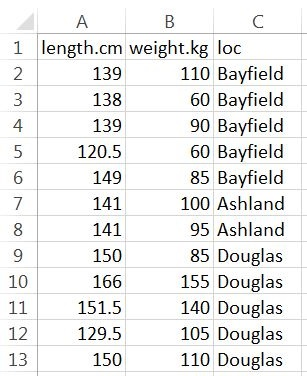
\includegraphics[width=1.5in]{Figs/Data_File_1.jpg}
\end{center}


\defn{data.frame}{A two-dimensional organization of variables (as columns, possibly of different data types) recorded on multiple individuals (as rows).}

\vspace{-12pt}
\warn{The columns of a data.frame correspond to variables and the rows of a data.frame correspond to individuals.}

Variable names must NOT contain spaces.  For example, don't use \var{total length} or \var{length (cm)}.  If you feel the need to have longer variable names, then separate the parts with a period (e.g., \var{length.cm}) or an underscore (e.g., \var{length\_cm}).  Furthermore, numerical measurements should NOT include units (e.g., don't use \verb"7 cm").  Finally, for categorical data, make sure that all categories are consistent (e.g., do not have a column that contains both \verb"bayfield" and \verb"Bayfield").

\warn{Variable names and data should not contain spaces.  An "\R{Error in scan}" message usually indicates spaces in the variable names or data.}

The spreadsheet is saved as a CSV file by selecting the \verb"File..Save As" menu item, which will produce the dialog box below. In this dialog box, change \verb"Save as type" to \verb"CSV (Comma delimited) (*.csv)" (you may have to scroll down), provide a file name (don't have any periods in the name besides for ``.csv'', which you should not have to type), select a location to save the file (don't forget this location!!), and press \verb"Save".  Two ``warning'' dialog boxes may then appear -- select \verb"OK" for the first and \verb"YES" for the second.  You can now close the spreadsheet file (you may be asked to save changes -- you should say \verb"No").
\begin{center}
  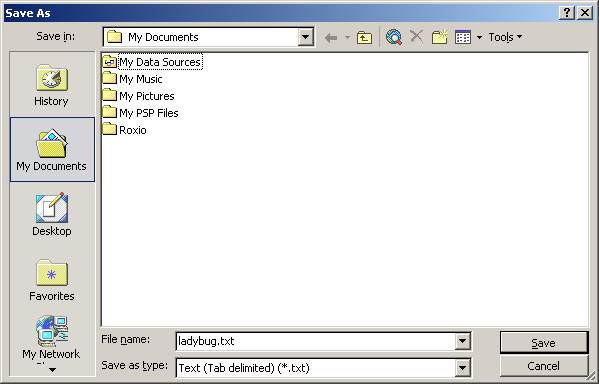
\includegraphics[width=3.5in]{Figs/Data_File_2.jpg}
\end{center}

The following steps are used to load the data in the CSV file into RStudio.

\begin{Itemize}
  \item Open RStudio.
  \item Open a new script by selecting the \verb"File", \verb"New File", \verb"R Script" menu items.
  \item Type \R{library(NCStats)} in the new script.
  \item Save this script by selecting the \verb"File", \verb"Save" menu items.  In the ensuing dialog box, navigate to the \textbf{exact same directory} where you saved the data, type a name for the file in the \verb"File name:" box (\textbf{do not use a period in this name!!}), and press \verb"Save".

\begin{center}
  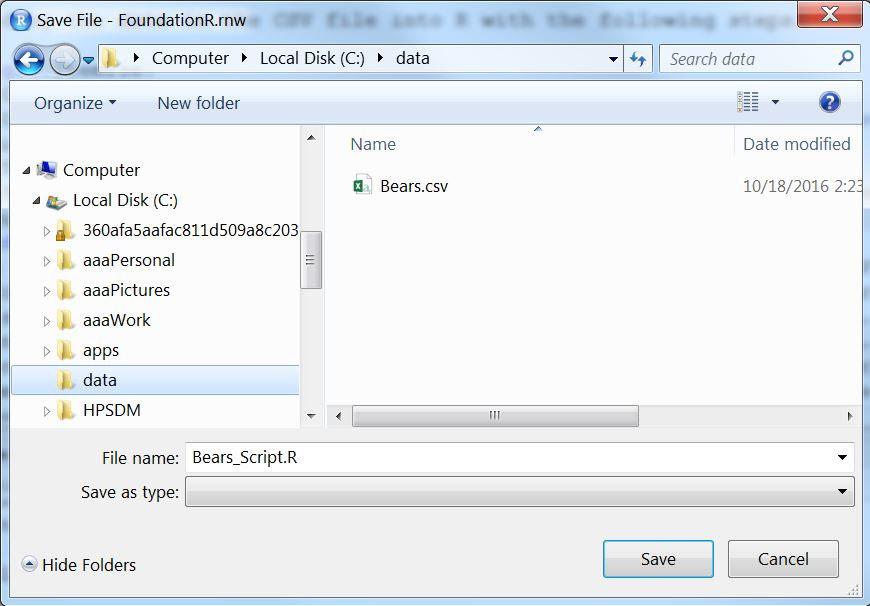
\includegraphics[width=3.5in]{Figs/Data_File_3.jpg}
\end{center}

  \item Set the working directory (tell R where the file is) with the \verb"Session", \verb"Set Working Directory ...", \verb"To Source File Location" menu items in RStudio.  RStudio will print an appropriate \R{setwd()} command to the console.  Copy this command from the console to the second line in your script.\footnote{Doing this will eliminate the need to manually select the menu options every time you want to run this script.}  For example, I stored the file created above in the \verb"C:/data" directory, so that RStudio will create this \R{setwd("C:/data")}.
  \item The CSV file is read into R by including the name of the file (in quotes) in \R{read.csv()}.  For example, \R{"Bears.csv"} is read into R and stored into an object called \R{bears} with \R{bears <- read.csv("Bears.csv")}.


  \item One should check the data in this object as descried in \sectref{sect:RViewdf} below
\end{Itemize}

\warn{Data stored in an external CSV file is read into R with \R{read.csv()}.}

It is important that each row of the data.frame correspond to one individual.  This is critically important when data are recorded for two different groups (e.g., for a two-sample t-test; see \modref{chap:tTest2}).  For example, the following data are methyl mercury levels recorded in mussels from two locations labeled as ``impacted'' and ``reference.''
\begin{Verbatim}
  impacted   0.011  0.054  0.056  0.095  0.051  0.077
  reference  0.031  0.040  0.029  0.066  0.018  0.042  0.044
\end{Verbatim}
To follow the ``one individual per row'' rule, these data are entered in stacked format where the ``reference'' data are stacked underneath the ``impacted'' data and a column is used to indicate to which group the individuals belong.  For example, the Excel file for data entry would look like the following

\begin{center}
  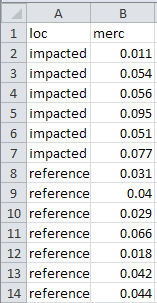
\includegraphics[width=1in]{Figs/StackedData.jpg}
\end{center}

\warn{Data files are constructed with data from only one individual in each row.}

\subsubsection*{Alternative Forms of Getting Data} \label{sect:RAltData}
\vspace{-12pt}
Some of the data files that you will use are provided on the \href{http://derekogle.com/NCMTH107/resources/data_107}{Data for MTH107} resource page of the class webpage.  In these cases, the data should be downloaded from the webpage and saved in the same directory or folder as your analysis script.  The downloaded file is then read into R in the same manner as described previously (i.e., set the working directory with \R{setwd()} and use \R{read.csv()}).

A few data files used in this book are supplied with R or the NCStats package.  These files are loaded with \R{data()}.  For example, the \dfile{iris} data file is loaded into R with
\begin{knitrout}
\definecolor{shadecolor}{rgb}{0.922, 0.922, 0.922}\color{fgcolor}\begin{kframe}
\begin{verbatim}
> data(iris)
\end{verbatim}
\end{kframe}
\end{knitrout}


\subsection{Working With Data Frames}  \label{sect:RWorkdf}
\vspace{-12pt}
\subsubsection{Viewing a Data Frame}  \label{sect:RViewdf}
\vspace{-12pt}
Many users are disoriented in RStudio because they cannot ``see'' their data in the same way that they see it in a spreadsheet program.  There are, however, several options for viewing your data.  First, you can type the name of the data.frame object to see its entire contents.
\begin{knitrout}
\definecolor{shadecolor}{rgb}{0.922, 0.922, 0.922}\color{fgcolor}\begin{kframe}
\begin{verbatim}
> bears
   length.cm weight.kg      loc
1      139.0       110 Bayfield
2      138.0        60 Bayfield
3      139.0        90 Bayfield
4      120.5        60 Bayfield
5      149.0        85 Bayfield
6      141.0       100  Ashland
7      141.0        95  Ashland
8      150.0        85  Douglas
9      166.0       155  Douglas
10     151.5       140  Douglas
11     129.5       105  Douglas
12     150.0       110  Douglas
\end{verbatim}
\end{kframe}
\end{knitrout}

Typing the name is adequate for small data.frames, but not useful for large data.frames.  The entire data.frame is opened in a separate window by double-clicking on the name of the data.frame in the \R{Environment} tab of RStudio.  Alternatively, the first and last three rows are viewed by including the data.frame object in \R{headtail()}.
\begin{knitrout}
\definecolor{shadecolor}{rgb}{0.922, 0.922, 0.922}\color{fgcolor}\begin{kframe}
\begin{verbatim}
> headtail(bears)
   length.cm weight.kg      loc
1      139.0       110 Bayfield
2      138.0        60 Bayfield
3      139.0        90 Bayfield
10     151.5       140  Douglas
11     129.5       105  Douglas
12     150.0       110  Douglas
\end{verbatim}
\end{kframe}
\end{knitrout}

In addition to viewing the contents, it is useful to examine the structure of the data.frame as returned from \R{str()}.  In this example, it is seen that three variables were recorded on 12 individuals.  The first variables -- \var{length.cm} and \var{weight.kg} -- are numerical measurements made on the bears.  The last variable -- \var{loc} -- is a factor variable that records the capture location for each bear.
\begin{knitrout}
\definecolor{shadecolor}{rgb}{0.922, 0.922, 0.922}\color{fgcolor}\begin{kframe}
\begin{verbatim}
> str(bears)
'data.frame':	12 obs. of  3 variables:
 $ length.cm: num  139 138 139 120 149 ...
 $ weight.kg: int  110 60 90 60 85 100 95 85 155 140 ...
 $ loc      : Factor w/ 3 levels "Ashland","Bayfield",..: 2 2 2 2 2 1 1 3 3 3 ...
\end{verbatim}
\end{kframe}
\end{knitrout}
The levels of the \var{loc} variable may be seen by including this variable (with the data.frame name) as the argument to \R{levels()}.
\begin{knitrout}
\definecolor{shadecolor}{rgb}{0.922, 0.922, 0.922}\color{fgcolor}\begin{kframe}
\begin{verbatim}
> levels(bears$loc)
[1] "Ashland"  "Bayfield" "Douglas" 
\end{verbatim}
\end{kframe}
\end{knitrout}

In the previous example, the \R{\$} notation was used to identify a particular variable (i.e., \R{loc}) within a data.frame (\R{bears}).  Think of variables as being nested inside data.frames and, thus, to access the variable you must first identify the data.frame in which it exists and then the name of the variable.  The \R{\$} simply separates the data.frame from the variable.
\begin{knitrout}
\definecolor{shadecolor}{rgb}{0.922, 0.922, 0.922}\color{fgcolor}\begin{kframe}
\begin{verbatim}
> bears$length.cm
 [1] 139.0 138.0 139.0 120.5 149.0 141.0 141.0 150.0 166.0 151.5 129.5 150.0
> bears$loc
 [1] Bayfield Bayfield Bayfield Bayfield Bayfield Ashland  Ashland  Douglas  Douglas 
[10] Douglas  Douglas  Douglas 
Levels: Ashland Bayfield Douglas
\end{verbatim}
\end{kframe}
\end{knitrout}

\warn{A dollar sign is ONLY used in R to separate the name of a data.frame from the name of a variable within that data.frame.}

\subsubsection{Selecting Individuals}  \label{sect:RSelectIndivs}
\vspace{-12pt}

In some instances, it may be important to select or exclude an individual from a data.frame.  Data.frames are two-dimensional objects that are indexed by a row and a column, in that order.  Positions within a data.frame are selected within paired square brackets.  For example, the item in the third row and second column of \R{bears} is selected below.
\begin{knitrout}
\definecolor{shadecolor}{rgb}{0.922, 0.922, 0.922}\color{fgcolor}\begin{kframe}
\begin{verbatim}
> bears[3,2]
[1] 90
\end{verbatim}
\end{kframe}
\end{knitrout}

\warn{Identifying the position of an item in an object is the ONLY time that square brackets are used in R.}

An entire row or column may be selected by omitting the other dimension.  For example, one could select the entire second column with \R{bears[,2]}, but this is also the \R{weight.kg} variable and is better selected, as shown above, with \R{bears\$weight.kg}.  As a better example, the entire third row is selected below (note that the column designation was omitted).
\begin{knitrout}
\definecolor{shadecolor}{rgb}{0.922, 0.922, 0.922}\color{fgcolor}\begin{kframe}
\begin{verbatim}
> bears[3,]
  length.cm weight.kg      loc
3       139        90 Bayfield
\end{verbatim}
\end{kframe}
\end{knitrout}

Multiple rows are selected by combining row indices together with \R{c()} (more about \R{c()} in \sectref{sect:RVectors}).  For example, the third, fifth, and eighth rows are selected below (again, the column index is omitted).
\begin{knitrout}
\definecolor{shadecolor}{rgb}{0.922, 0.922, 0.922}\color{fgcolor}\begin{kframe}
\begin{verbatim}
> bears[c(3,5,8),]
  length.cm weight.kg      loc
3       139        90 Bayfield
5       149        85 Bayfield
8       150        85  Douglas
\end{verbatim}
\end{kframe}
\end{knitrout}

Finally, rows can be excluded by preceding the row indices with a negative sign.
\begin{knitrout}
\definecolor{shadecolor}{rgb}{0.922, 0.922, 0.922}\color{fgcolor}\begin{kframe}
\begin{verbatim}
> bears[-c(3,5,8,10,12),]
   length.cm weight.kg      loc
1      139.0       110 Bayfield
2      138.0        60 Bayfield
4      120.5        60 Bayfield
6      141.0       100  Ashland
7      141.0        95  Ashland
9      166.0       155  Douglas
11     129.5       105  Douglas
\end{verbatim}
\end{kframe}
\end{knitrout}

\vspace{-12pt}
\subsubsection{Filtering a data.frame}  \label{sect:RSubsetdf}
\vspace{-12pt}
It is common to create a new data.frame that contains only some of the individuals from an existing data.frame.  For example, a researcher may want a data.frame of only bears captured in Bayfield County or bears that weighed more than 100 kg.  The process of creating the newer, smaller data.frame is called filtering (or subsetting) and is accomplished with \R{filterD()}.  The \R{filterD()} function requires the original data.frame as the first argument and a condition statement as the second argument.  The condition statement is used to either include or exclude individuals from the original data.frame.  Condition statements consist of the name of a variable in the original data.frame, a comparison operator, and a comparison value \tabrefp{tab:RSubsetConditions}.  The result from \R{filterD()} should be assigned to an object, which is then the name of the new data.frame.

\warn{\R{filterD()} is used to create a new data.frame that consists of individuals selected by some criterion from an existing data.frame.}

\begin{table}[htbp]
  \caption{Condition operators used in \R{filterD()} and their results.  Note that \emph{variable} generically represents a variable in the original data.frame and \emph{value} is a generic value or level.  Both \emph{variable} and \emph{value} would be replaced with specific items.}  \label{tab:RSubsetConditions}
  \centering
\begin{tabular}{cc}
\hline\hline
Condition Operator &  Individuals Returned from Original Data Frame \\
\hline
\widen{-1}{6}{\emph{variable}} $==$ \emph{value} & all individual that are \textbf{equal} to the given value \\
\widen{-1}{5}{\emph{variable}} $!=$ \emph{value} & all individuals that are \textbf{NOT equal} to the given value \\
\widen{-1}{5}{\emph{variable}} $>$ \emph{value} & all individuals that are \textbf{greater than} the given value \\
\widen{-1}{5}{\emph{variable}} $>=$ \emph{value} & all individuals that are \textbf{greater than or equal} to the given value \\
\widen{-1}{5}{\emph{variable}} $<$ \emph{value} & all individuals that are \textbf{less than} the given value \\
\widen{-1}{5}{\emph{variable}} $<=$ \emph{value} & all individuals that are \textbf{less than or equal} to the given value \\
\widen{-1}{5}{\emph{condition}}, \emph{condition} & all individuals that \textbf{meet both conditions} \\
\widen{-2}{6}{\emph{condition}} $|$ \emph{condition} & all individuals that \textbf{meet one or both conditions}\footnote{Note that this ``or'' operator is a ``vertical line'' which is typed with the shift-backslash key.} \\
\hline\hline
\end{tabular}
\end{table}

\vspace{18pt}
The following are examples of new data.frames created from \var{bears}.  The name of the new data.frame (i.e., object to the left of the assignment operator) can be any valid object name.  As demonstrated below, the new data.frame (or its structure) should be examined after each filtering to ensure that the data.frame actually contains the items that you desire.

\begin{itemize}
  \item Only individuals from \emph{Bayfield} county.
\begin{knitrout}
\definecolor{shadecolor}{rgb}{0.922, 0.922, 0.922}\color{fgcolor}\begin{kframe}
\begin{verbatim}
> bf <- filterD(bears,loc=="Bayfield")
> bf
  length.cm weight.kg      loc
1     139.0       110 Bayfield
2     138.0        60 Bayfield
3     139.0        90 Bayfield
4     120.5        60 Bayfield
5     149.0        85 Bayfield
\end{verbatim}
\end{kframe}
\end{knitrout}

  \item Individuals from both \emph{Bayfield} and \emph{Ashland} counties.
\begin{knitrout}
\definecolor{shadecolor}{rgb}{0.922, 0.922, 0.922}\color{fgcolor}\begin{kframe}
\begin{verbatim}
> bfash <- filterD(bears,loc %in% c("Bayfield","Ashland"))
> bfash
  length.cm weight.kg      loc
1     139.0       110 Bayfield
2     138.0        60 Bayfield
3     139.0        90 Bayfield
4     120.5        60 Bayfield
5     149.0        85 Bayfield
6     141.0       100  Ashland
7     141.0        95  Ashland
\end{verbatim}
\end{kframe}
\end{knitrout}

  \item Individuals with a weight greater than 100 kg.
\begin{knitrout}
\definecolor{shadecolor}{rgb}{0.922, 0.922, 0.922}\color{fgcolor}\begin{kframe}
\begin{verbatim}
> gt100 <- filterD(bears,weight.kg>100)
> gt100
  length.cm weight.kg      loc
1     139.0       110 Bayfield
2     166.0       155  Douglas
3     151.5       140  Douglas
4     129.5       105  Douglas
5     150.0       110  Douglas
\end{verbatim}
\end{kframe}
\end{knitrout}

  \item Individuals from \emph{Douglas} County that weigh at least 150 kg.
\begin{knitrout}
\definecolor{shadecolor}{rgb}{0.922, 0.922, 0.922}\color{fgcolor}\begin{kframe}
\begin{verbatim}
> do150 <- filterD(bears,loc=="Douglas",weight.kg>=150)
> do150
  length.cm weight.kg     loc
1       166       155 Douglas
\end{verbatim}
\end{kframe}
\end{knitrout}
\end{itemize}

\warn{View or ``structure'' the data.frame from \R{filterD()} to be sure that it contains data.}

\begin{exsection}
  \item \label{revex:BasicsDataFrame1} \rhw{} Two students at Seattle Community College made biometric measurements on 25 Douglas fir (\emph{Pseudotsuga menziesii}) trees in the lowlands of western Washington.  The variables recorded in the \href{https://raw.githubusercontent.com/droglenc/NCData/master/DougFirBiometrics.csv}{DougFirBiometrics.csv} file are a unique tree identifier (\var{tree}), the observer's name (\var{observer}; either ``Ingrid'' or ``Dylan''), the circumference at breast height (meters; \var{circ}), the height to the eye of the observer (meters; \var{eyeht}), the horizontal distance between observer and tree (meters; \var{horizdist}), the angle between observer and top of tree (degrees; \var{angle}), and the estimated height of tree (meters; \var{height}) using right-angle trigonometry. \ansref{ans:BasicsDataFrame1}
  \begin{Enumerate}
    \item Read this data file into an object called \R{DF}.
    \item Examine the structure of this data.frame.
    \item Show all measurements made on the third tree. [Do not do this manually; use R code.]
    \item Show all estimated tree heights.
    \item Show the estimated tree height for the fifth tree.
    \item Show all measurements for all trees measured by ``Ingrid''.  [HINT: use filtering.]
    \item Show all estimated tree heights for all trees measured by ``Dylan''.  [HINT: use filtering.]
    \item Show all measurements for tree heights less than 10 m.  [HINT: use filtering.]
    \item Show all measurements for tree heights greater than 10 m and circumference less than 1 m.  [HINT: use filtering.]
  \end{Enumerate}
\end{exsection}

\vspace{-12pt}
\subsection{Vectors}  \label{sect:RVectors}
\vspace{-12pt}

Data.frames are the primary structure in which to store real data.  However, much simpler situations that don't require a data.frame may arise.  In R, items of the same data type \sectrefp{sect:RDataTypes} are stored in a one-dimensional ``list'' called a \emph{vector}.  Vectors are usually displayed in one row (with many columns), but they may also be thought of as a single column (with many rows).  Items are entered into a vector with \R{c()}, where the individual arguments are specific numbers, characters, or logical values.\footnote{Note that \R{c} comes from the word ``concatenate.''}  Items for a vector of characters must be contained within paired quotes.
\begin{knitrout}
\definecolor{shadecolor}{rgb}{0.922, 0.922, 0.922}\color{fgcolor}\begin{kframe}
\begin{verbatim}
> ( v <- c(1,2,5) )
[1] 1 2 5
> ( y <- c("Iowa","Minnesota","Wisconsin") )
[1] "Iowa"      "Minnesota" "Wisconsin"
\end{verbatim}
\end{kframe}
\end{knitrout}

\defn{Vector}{A one-dimensional list of items of the same data type.  The primary information storage unit in R.}

Single variables from a data.frame are vectors.  Vectors that are not extracted from a data.frame will only be used in this course for very simple lists of items, usually as arguments in a function.
\begin{knitrout}
\definecolor{shadecolor}{rgb}{0.922, 0.922, 0.922}\color{fgcolor}\begin{kframe}
\begin{verbatim}
> bears$length.cm
 [1] 139.0 138.0 139.0 120.5 149.0 141.0 141.0 150.0 166.0 151.5 129.5 150.0
\end{verbatim}
\end{kframe}
\end{knitrout}

\warn{The columns of a data.frame are accessed with the name of the data.frame, a dollar sign, and then the name of the variable -- i.e., generically, \R{dataframe\$varname}.}


\begin{exsection}
  \item \label{revex:BasicsData1}\rhw{} Create a vector called \var{h} that contains nine heights of people. \ansref{ans:BasicsData1}
  \item \label{revex:BasicsData2}\rhw{} Create a vector called \var{w} that contains nine weights of people. \ansref{ans:BasicsData2}
  \item \label{revex:BasicsData3}\rhw{} Create a vector called \var{hc} that contains nine hair colors of people. \ansref{ans:BasicsData3}
  \item \label{revex:BasicsData4}\rhw{} Create a vector called \var{m} that contains nine logical values (=\R{TRUE} if male). \ansref{ans:BasicsData4}
  \item \label{revex:BasicsData5}\rhw{} Using the vectors from the previous questions,  \ansref{ans:BasicsData5}
  \begin{Enumerate}
    \item ... create the largest possible data.frame (use \R{data.frame()}).
    \item ... identify the height of the third individual of this data.frame.
    \item ... identify the hair color for the sixth individual of this data.frame.
  \end{Enumerate}
\end{exsection}

    \part{Exploratory Data Analysis}



\chapter{Univariate EDA - Quantitative} \label{chap:UnivEDAQuant}
\begin{ChapObj}{\boxwidth}
  \textbf{Objectives:}
  \begin{Enumerate}
    \item Construct histograms with quantitative data,
    \item Use graphs to describe the shape of a distribution, and
    \item Use graphs to describe outliers in a distribution.
    \item Calculate summary statistics for measuring the center of quantitative data,
    \item Calculate summary statistics for measuring the dispersion of quantitative data,
    \item Describe the underlying differences in how the different statistics measure center and dispersion,
    \item Identify which summary statistics are appropriate in a given situation, and
    \item Construct an appropriate overall numerical summary.
  \end{Enumerate}
\end{ChapObj}

\minitoc
\newpage

\lettrine{O}{nce data have been collected} \modrefp{chap:DataProd}, it is important to develop a ``feel'' for the data, to identify what types of values each variable takes, and to determine if there are any ``issues'' in the data.  This first step in a statistical analysis is called \textsc{Exploratory Data Analysis} (EDA).  We will begin by examining the distribution of each variable by itself, called a univariate EDA, and then examine pairs of variables, called a bivariate EDA (see Modules \ref{chap:BivEDAQuant} and \ref{chap:BivEDACat}). Additionally, the methods employed differ for quantitative and categorical variables. Quantitative variables are the focus of this module, whereas categorical variables are the focus of \modref{chap:UnivEDACat}.

\vspace{-6pt}
\section{Items to Describe}
\vspace{-12pt}
A univariate EDA for a quantitative variable is concerned with describing the distribution of the values for that variable; i.e., describing what values occurred and how often those values occurred.\index{EDA!Univariate!Quantitative}  Specifically, the distribution is described by four specific attributes:

\vspace{-12pt}
\begin{Enumerate}
  \item \textbf{shape} of the distribution,
  \item presence of \textbf{outliers},
  \item \textbf{center} of the distribution, and
  \item \textbf{dispersion} or spread of the distribution.
\end{Enumerate}
\vspace{-8pt}

Graphs are used to identify shape and the presence of outliers and to get a general feel for center and dispersion.  However, numerical summaries are used to specifically describe center and dispersion of the data.

\vspace{-6pt}
\warn{Shape, center, dispersion, and outliers are described for each quantitative variable.}

\vspace{-12pt}
\warn{Shape and outliers are described from graphs; center and dispersion are describe with numerical summaries.}

Three primary data sets will be explored throughout this module.

\vspace{-12pt}
\begin{Itemize}
  \item Measurements of water consumption in one hour by mice \tabrefp{tab:MouseData}.\footnote{See \sectref{sect:REnterData} for how to enter these data into R.}
  \item Richter scale recordings for 15 major earthquakes \tabrefp{tab:EQData}.
  \item The number of days of ice cover at ice gauge station 9004 in Lake Superior (data in \href{https://raw.githubusercontent.com/droglenc/NCData/master/LakeSuperiorIce.csv}{LakeSuperiorIce.csv}).\footnote{See \sectref{sect:RAltData} for a description of how to access these data. These datat are originally from the \href{http://www.nsidc.org/}{National Snow and Ice Data Center}.}  The \var{days} variable is the total number of days of ice cover at this site for nearly every ice season from 1955-56 to 1996-97 (three years were missing).  These data are loaded into \R{LSI} below.
\vspace{-6pt}
\begin{knitrout}
\definecolor{shadecolor}{rgb}{0.922, 0.922, 0.922}\color{fgcolor}\begin{kframe}
\begin{verbatim}
> LSI <- read.csv("data/LakeSuperiorIce.csv")
\end{verbatim}
\end{kframe}
\end{knitrout}
\end{Itemize}

% latex table generated in R 3.3.3 by xtable 1.8-2 package
% Wed Apr 26 20:49:43 2017
\begin{table}[ht]
\centering
\caption{Amount of water consumed (in ml) in one hour by a sample of mice.} 
\label{tab:MouseData}
\begin{tabular}{rrrrrrrrrrrrrrr}
   \hline
10.6 & 14.1 & 13.7 & 15.2 & 15.4 & 12.5 & 12.9 & 14.3 & 13.0 & 16.6 & 11.5 & 9.4 & 16.5 & 13.7 & 14.7 \\ 
  12.6 & 12.0 & 14.0 & 10.0 & 18.2 & 18.4 & 17.4 & 11.1 & 15.8 & 15.8 & 16.6 & 11.4 & 17.0 & 13.6 & 13.5 \\ 
   \hline
\end{tabular}
\end{table}


% latex table generated in R 3.3.3 by xtable 1.8-2 package
% Wed Apr 26 20:49:43 2017
\begin{table}[ht]
\centering
\caption{Richter scale recordings for 15 major earthquakes.} 
\label{tab:EQData}
\begin{tabular}{rrrrrrrrrrrrrrr}
   \hline
5.5 & 6.3 & 6.5 & 6.5 & 6.8 & 6.8 & 6.9 & 7.1 & 7.3 & 7.3 & 7.7 & 7.7 & 7.7 & 7.8 & 8.1 \\ 
   \hline
\end{tabular}
\end{table}


\section{Histograms}\index{Histogram!Construction}\index{Sample Distribution!Histogram}
\vspace{-8pt}
\subsection{General Construction}
\vspace{-8pt}
A histogram is a plot of the frequency of occurrence of individuals (y-axis) in classes of values of the variable (x-axis).  The steps for constructing a histogram from raw data are:
\vspace{-6pt}
\begin{Enumerate}
  \item Create categorical classes of values for the variable of interest,
  \item Count the frequency of individuals in each class,
  \item Construct a graph template with values of the variable on the x-axis and frequency of individuals on the y-axis, and
  \item Draw bars on the graph that are as wide as the class of values and as tall as the frequency of individuals.
\end{Enumerate}

These steps are illustrated with the mouse water consumption data. The easiest way to create a list of classes is to divide the difference between the maximum and minimum values in the data by a ``nice'' number near eight to ten, and then round up to make classes that are easy to work with. The ``nice'' number between eight and ten is chosen to make the division easy and will be the number of classes.  In this example, the range of values is 18.4-9.4 = 9.0.  A ``nice'' value between eight and ten to divide this range by is nine.  Thus, the classes of data should be one unit wide and, for ease, will begin at 9 mm \tabrefp{tab:MouseFreqTable}.

\begin{table}[htbp]
  \caption{Frequency table of mouse consumption values in one-unit classes.}
  \label{tab:MouseFreqTable}
    \begin{Verbatim}[xleftmargin=25mm]
Class     Frequency
 9.0- 9.9      1
10.0-10.9      2
11.0-11.9      3
12.0-12.9      4
13.0-13.9      5
14.0-14.9      4
15.0-15.9      4
16.0-16.9      3
17.0-17.9      2
18.0-18.9      2
    \end{Verbatim}
\end{table}

The number of individuals with a value of the variable in each class is called a frequency and are shown in the second column of \tabref{tab:MouseFreqTable}. The plot is prepared with values of the classes forming the x-axis and frequencies forming the y-axis (\figref{fig:MouseHist1}-Left).  The first bar added to this skeleton plot has the bottom-left corner at 9 and the bottom-right corner at 10 on the x-axis, and a height equal to the frequency of individuals in the 9 to 9.9 class (\figref{fig:MouseHist1}-Center).  A second bar is then added with the bottom-left corner at 10 and the bottom-right corner at 11 on the x-axis, and a height equal to the frequency of individuals in the 10 to 10.9 class (\figref{fig:MouseHist1}-Right).  This process is continued with the remaining classes until the full histogram is constructed \figrefp{fig:MouseHist2}.

\begin{knitrout}
\definecolor{shadecolor}{rgb}{0.922, 0.922, 0.922}\color{fgcolor}\begin{figure}[hbtp]

{\centering 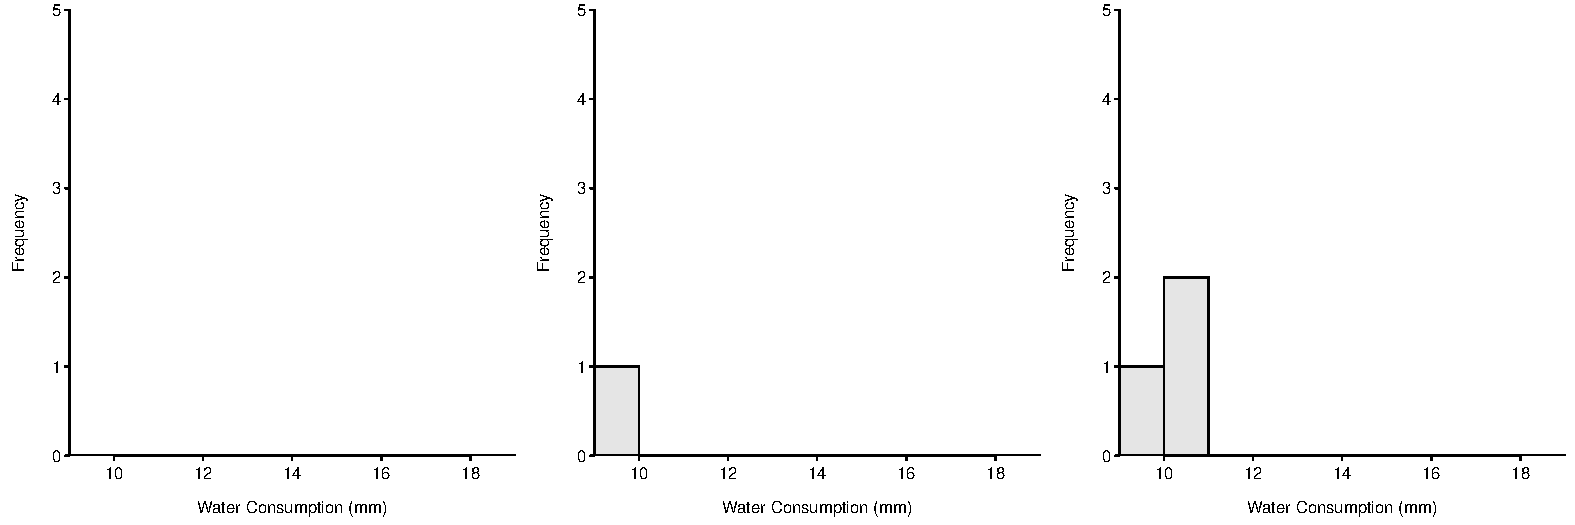
\includegraphics[width=.95\linewidth]{Figs/MouseHist1-1} 

}

\caption[Steps illustrating the development of a histogram]{Steps illustrating the development of a histogram.}\label{fig:MouseHist1}
\end{figure}


\end{knitrout}

\vspace{24pt}  % handles an overlapping problem with the floats

\begin{knitrout}
\definecolor{shadecolor}{rgb}{0.922, 0.922, 0.922}\color{fgcolor}\begin{figure}[hbtp]

{\centering 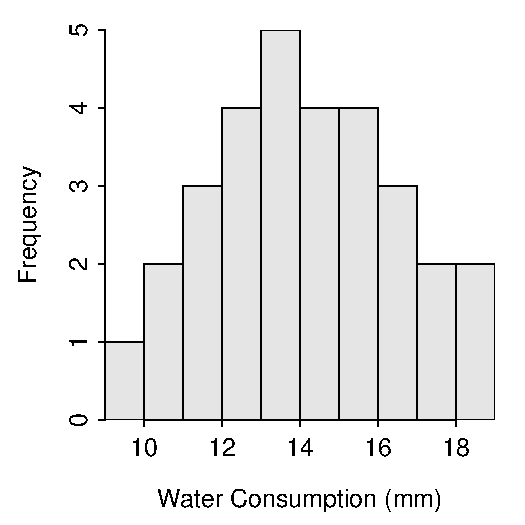
\includegraphics[width=.4\linewidth]{Figs/MouseHist2-1} 

}

\caption[Histogram of water consumption (mm) by mice]{Histogram of water consumption (mm) by mice.}\label{fig:MouseHist2}
\end{figure}


\end{knitrout}

Ideally eight to ten classes (i.e., bars) are used to construct a histogram.  Too many or too few bars make it difficult to identify the shape and may lead to different interpretations.  A dramatic example of the effect of changing the number of classes is seen in histograms of the length of eruptions for the Old Faithful geyser \figrefp{fig:histOF}.

\begin{knitrout}
\definecolor{shadecolor}{rgb}{0.922, 0.922, 0.922}\color{fgcolor}


















































\begin{figure}[hbtp]

{\centering \animategraphics[width=.4\linewidth,controls,palindrome,autoplay]{1}{Figs/histOF-}{1}{52}

}

\caption[Histogram of length (minutes) of eruptions for Old Faitfhul geyser with varying number of classes]{Histogram of length (minutes) of eruptions for Old Faitfhul geyser with varying number of classes.}\label{fig:histOF}
\end{figure}


\end{knitrout}

\subsection{Histograms in R}
A simple (by default) histogram is constructed with \R{hist()} using a one-sided formula of the form \R{\TILDE quant}, where \R{quant} generically represents the quantitative variable, and the corresponding data frame in \R{data=}.  The x-axis label may be improved from the default value by including a label in \R{xlab=}.\footnote{\R{xlab=} is for the ``x-axis label.''}  The width of the classes may be controlled by including a class width in \R{w=}.\footnote{The endpoints for the classes may also be set by giving a vector of endpoints to \R{breaks=}.}

\begin{knitrout}
\definecolor{shadecolor}{rgb}{0.922, 0.922, 0.922}\color{fgcolor}\begin{kframe}
\begin{verbatim}
> hist(~days,data=LSI,xlab="Days of Ice Cover")      # Fig 5.4-Left
> hist(~days,data=LSI,xlab="Days of Ice Cover",w=20) # Fig 5.4-Right
\end{verbatim}
\end{kframe}\begin{figure}[hbtp]

{\centering 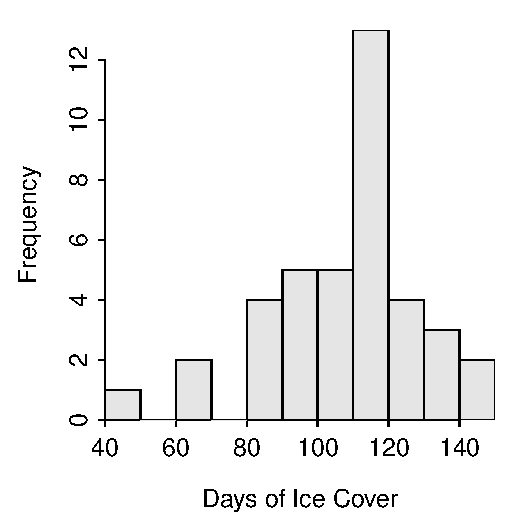
\includegraphics[width=.4\linewidth]{Figs/Histogram1-1} 
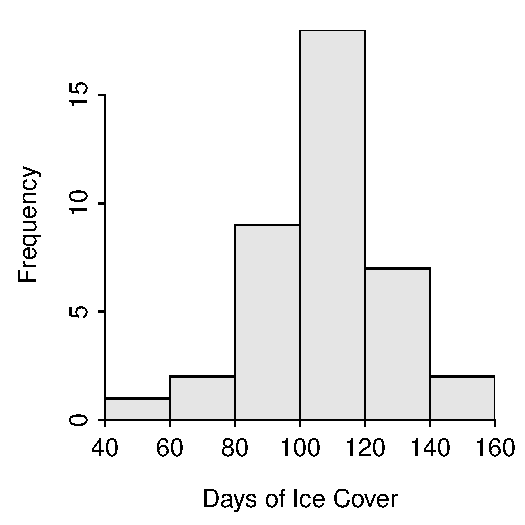
\includegraphics[width=.4\linewidth]{Figs/Histogram1-2} 

}

\caption[Histograms of the duration of ice cover at ice gauge 9004 in Lake Superior using the default class widths (Left) and widths of 20 days (Right)]{Histograms of the duration of ice cover at ice gauge 9004 in Lake Superior using the default class widths (Left) and widths of 20 days (Right).}\label{fig:Histogram1}
\end{figure}


\end{knitrout}

\warn{The default histogram should be modified by properly labeling the x-axis and possibly changing the class width.}

\begin{exsection}
  \item \label{revex:quEDAHistVar} Histograms are constructed from what type of variables? \ansref{ans:quEDAHistVar}
  \item \label{revex:quEDAHistX} What type of values are plotted on the x-axis of a histogram? \ansref{ans:quEDAHistX}
  \item \label{revex:quEDAHistY} What type of values are plotted on the y-axis of a histogram? \ansref{ans:quEDAHistY}
  \item \label{revex:quEDAHistBins} What is the ideal number of bars on a histogram? \ansref{ans:quEDAHistBins}
  \item \label{revex:quEDACreatPhosph} \rhw{} The table below contains the concentrations (International Units per liter) of creatine phosphokinase (an enzyme related to muscle and brain functions) in 36 male volunteers.  Construct a histogram from these data.  [HINT: Load data from a CSV file as in \sectref{sect:REnterData}.]\ansref{ans:quEDACreatPhosph}
    \begin{Verbatim}[xleftmargin=5mm]
121  82 100 151  68  58  95 145  64 119 104 110 113 118 203  62  83  67
201 101 163  84  57 139  60  78  94  93  92 110  25 123  70  48  95  42
    \end{Verbatim}
  \item \label{revex:quEDAAirPolln} \rhw{} The table below contains the carbon monoxide levels (ppm) arising from one of the stacks for an oil refinery northeast of San Francisco between April 16 and May 16, 1993. The measurements were submitted as evidence for establishing a baseline to the Bay Area Air Quality Management District (BAAQMD).\footnote{BAAQMD personnel had also made nine independent measurements of the carbon monoxide from this same stack over the period from September 11, 1990, to March 30, 1993, (which are not shown).}  Construct a histogram from these data.  [HINT: Load data from a CSV file as in \sectref{sect:REnterData}.]\ansref{ans:quEDAAirPolln}
    \begin{Verbatim}[xleftmargin=5mm]
30 30 34 36 37 38 40 42 43  43  45  52  55  58 58 58
59 63 63 71 75 85 86 86 99 102 102 141 153 261 21
    \end{Verbatim}
\end{exsection}

\vspace{-24pt}
\section{Interpreting Shape}\index{Histogram!Interpretation}
\vspace{-12pt}
A histogram has two tails -- a left-tail for smaller or more negative values and a right-tail for larger or more positive values.  The relative appearance of these two tails is used to identify three different shapes of distributions -- symmetric, left-skewed, and right-skewed.\index{Shape}\index{Symmetric}\index{Skewed}  If the left- and right-tail of a histogram are equal in shape (length and height), then the distribution is said to be \textbf{symmetric}.  Perfectly symmetric distributions rarely occur in ``real-life.''  Therefore, if the left- and right-tail are approximately equal in shape, then the distribution is \textbf{approximately symmetric}.  If the left-tail of the histogram is stretched out or, alternatively, the left-tail is longer and flatter than the right-tail, then the distribution is negatively- or \textbf{left-skewed}.  If the right-tail of the histogram is stretched out or, alternatively, the right-tail is longer and flatter than the left-tail, then the distribution is positively- or \textbf{right-skewed}.  The type of skew is defined by the longer tail; a longer right-tail means the distribution is right-skewed and a longer left-tail means it is left-skewed.  Examples of each shape are shown in \figref{fig:ShapeExamples}.

\begin{knitrout}
\definecolor{shadecolor}{rgb}{0.922, 0.922, 0.922}\color{fgcolor}\begin{figure}[hbtp]

{\centering 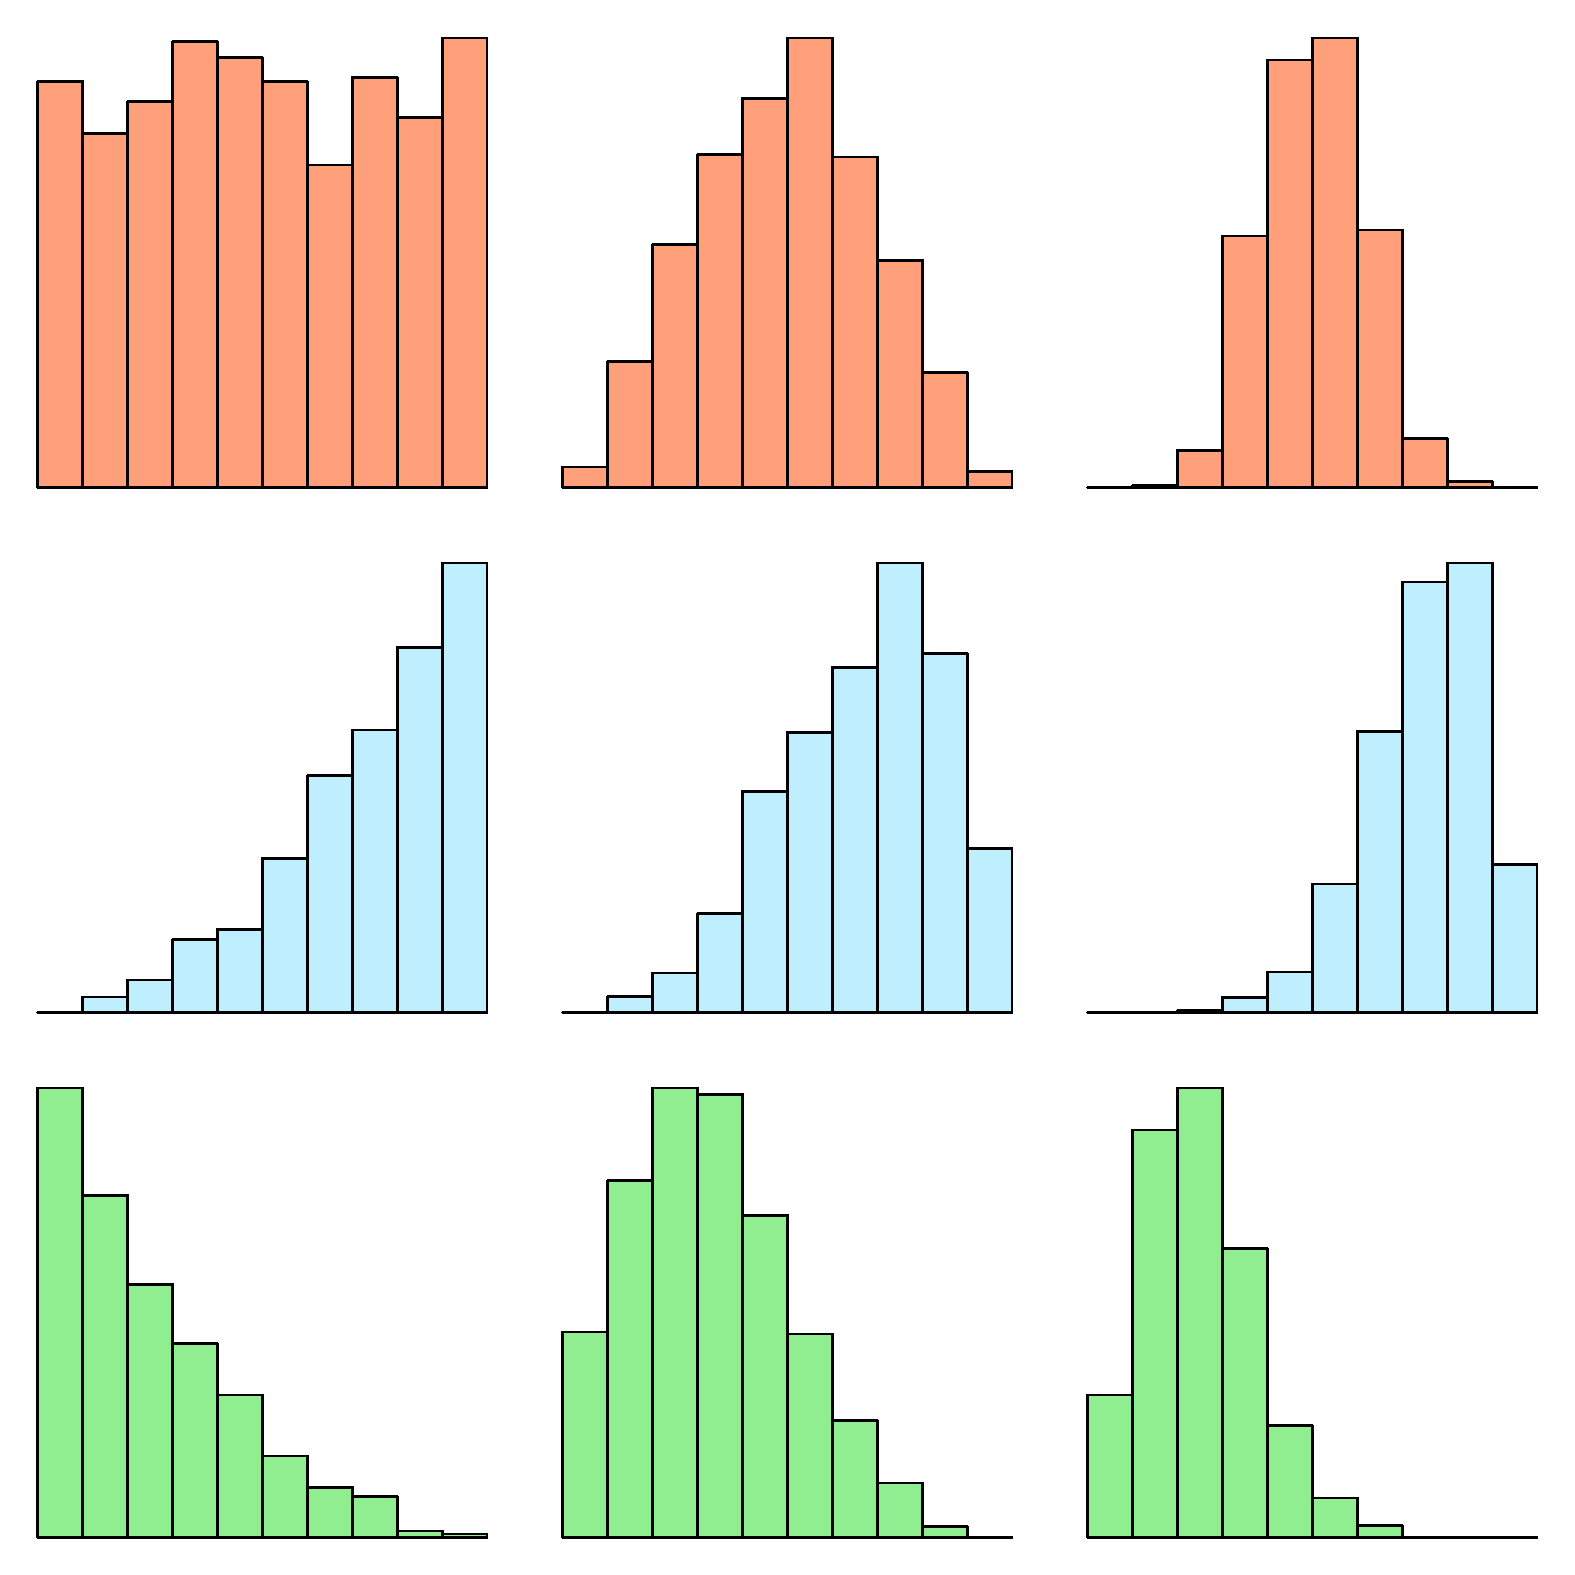
\includegraphics[width=.7\linewidth]{Figs/ShapeExamples-1} 

}

\caption[Examples of approximately symmetric (top, red), left-skewed (middle, blue), and right-skewed (bottom, green) histograms]{Examples of approximately symmetric (top, red), left-skewed (middle, blue), and right-skewed (bottom, green) histograms.  Note that the axes labels were removed to focus attention on the shape of the histograms.  Each histogram was constructed from n=1000 individuals and the x-axis range is from 0 to 1.}\label{fig:ShapeExamples}
\end{figure}


\end{knitrout}

\defn{Symmetric}{The left- and right-tail of a distribution are nearly the same in length and height.}

\vspace{-12pt}
\defn{Left-skewed}{The left-tail of a distribution is longer or more drawn out than the right-tail.}

\vspace{-12pt}
\defn{Right-skewed}{The right-tail of a distribution is longer or more drawn out than the left-tail.}

\vspace{-12pt}
\warn{The longer tail defines the type of skew.}

In practice, these labels form a continuum.  For example, a perfectly symmetric distribution is rare.  However, in the many cases of an asymmetric distribution, it is a fine line between calling the shape approximately symmetric or one of the skewed distributions.

\vspace{-12pt}
\warn{Symmetric, left-skewed, and right-skewed descriptors are guides; many ``real'' distributions will not fall neatly into these categories.}


\section{Interpreting Outliers}\index{Outlier}\index{Histogram!Interpretation}
\vspace{-12pt}
An outlier is an individual whose value is widely separated from the main cluster of values in the sample.  On histograms, outliers appear as bars that are separated from the main cluster of bars by ``white space'' or areas with no bars \figrefp{fig:OutlierExHist}.  In general, outliers must be on the margins of the histogram, should be separated by one or two missing bars, and should only be one or two individuals.

\begin{knitrout}
\definecolor{shadecolor}{rgb}{0.922, 0.922, 0.922}\color{fgcolor}\begin{figure}[hbtp]

{\centering 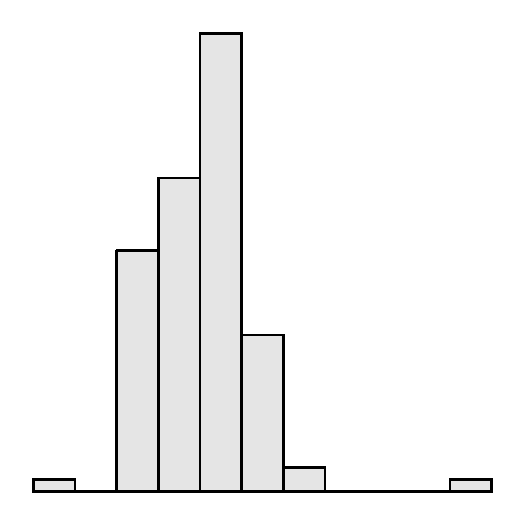
\includegraphics[width=.4\linewidth]{Figs/OutlierExHist-1} 

}

\caption[Example histogram with an outlier to the right]{Example histogram with an outlier to the right.}\label{fig:OutlierExHist}
\end{figure}


\end{knitrout}

\defn{Outlier}{An individual whose value is widely separated from the main cluster of values in the sample.}

An outlier may occur as a result of human error in the sampling process.  If this is the case, then the value should be corrected or removed.  Other times an outlier may be an individual that was not part of the population of interest -- e.g., an adult animal that was sampled when only immature animals were being considered.  In this case, the individual's value should be removed from the sample.  Still other times, an outlier is part of the population and should generally not be removed from the sample. In fact you may wish to highlight an outlier as an interesting observation! Regardless, it is important that you construct a histogram to determine if outliers are present or not.

Don't let outliers completely influence how you define the shape of a distribution.  For example, if the main cluster of values is approximately symmetric and there is one outlier to the right of the main cluster (as illustrated in \figref{fig:OutlierExHist}), \textbf{DON'T} call the distribution right-skewed.  You should describe this distribution as approximately symmetric with an outlier to the right.

\warn{Not all outliers warrant removal from your sample.}

\vspace{-12pt}
\warn{Don't let outliers completely influence how you define the shape of a distribution.}

\vspace{24pt}
\begin{exsection}
  \item \label{revex:quEDALSkew} What is a distribution with a long left-tail called? \ansref{ans:quEDALSkew}
  \item \label{revex:quEDARSkew} What is a distribution with a long right-tail called? \ansref{ans:quEDARSkew}
  \item \label{revex:quEDALSkewg} What is the shape of the distribution on the left below? \ansref{ans:quEDALSkewg}


\begin{center}
  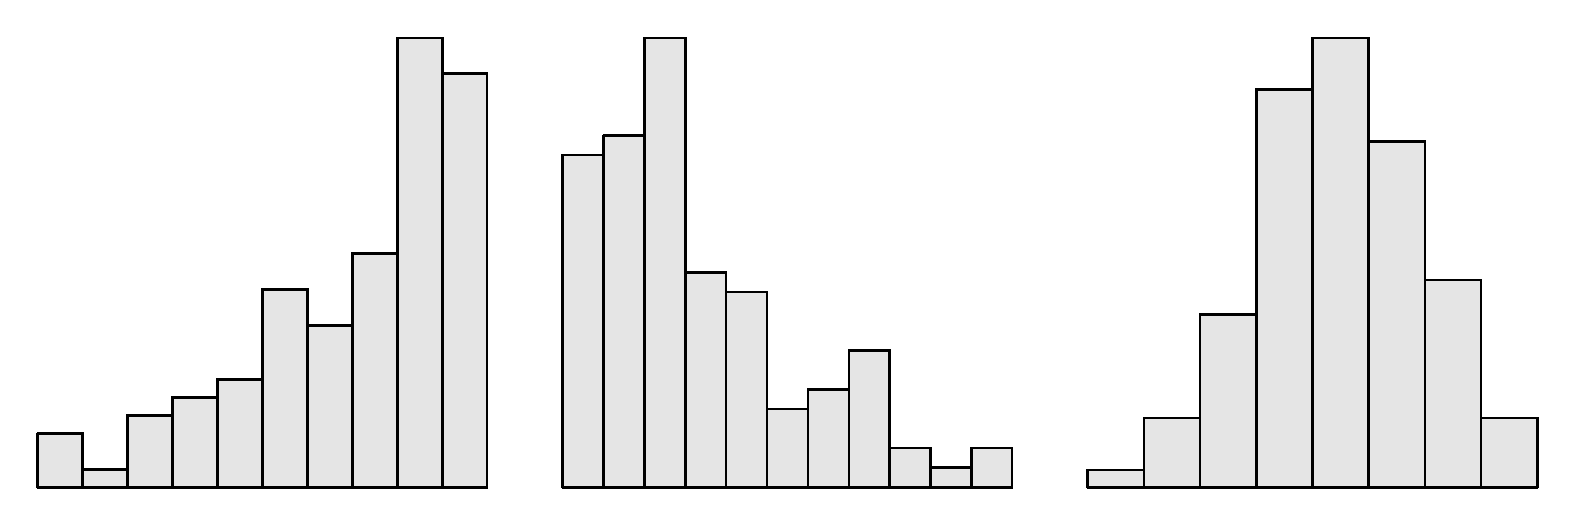
\includegraphics[width=5in]{Figs/HistQuest-1}
\end{center}
  \item \label{revex:quEDASymg} What is the shape of the distribution in the center above? \ansref{ans:quEDASymg}
  \item \label{revex:quEDARSkewg} What is the shape of the distribution on the right above? \ansref{ans:quEDARSkewg}
  \item \label{revex:quEDAlead} Comment on the shape and presence of outliers in \figref{fig:KreherParkPbhist}. \ansref{ans:quEDAlead}
\end{exsection}


\section{Measures of Center} \label{sec:quEDACenter}
There are three common methods to measure the center of a distribution: the mode, median, and mean.\index{Center}  The median and mean are the most widely used methods.  The choice of which method to use depends, in part, on the shape of the distribution, the presence of outliers, and your purpose.

The modes, medians, and means computed in this section are summary statistics -- i.e., they are computations from individuals in a sample.  Thus, they should specifically be called the sample mode, sample median, and sample mean.  The mode, median, and mean can also be computed from every individual in the population, if it is known.  The computed values would then be parameters and would be called the population mode, population median, and population mean.  See \sectref{sect:IVPPSS} for clarification on the differences between populations and samples and parameters and statistics.

\warn{Three measures of the center of a distribution are the mode, median, and mean.}

\vspace{-12pt}
\warn{Measures of center computed from individuals in a sample are preceded by ``sample''; those computed from all individuals in a population are preceded by ``population.''}

\subsection{Mode}
The mode is the value that occurs most often in a data set.\index{Mode}  If the variable is continuous, then the modal class is the class of values that occurs most often in a data set.  In other words, it is the class that forms the peak of a distribution.  For example, in the mouse water consumption data \figrefp{fig:MouseHist2} the modal class is 13.0-13.9.  Some data sets may have two ``humps,'' where each ``hump'' is considered a mode and the distribution is said to be \textbf{bimodal}.

\defn{Mode}{The value or class of values that occurs most often in a data set.}

\vspace{-12pt}
\defn{Bimodal}{The shape of a distribution with two peaks or ``humps.''}

\subsection{Median} \label{sec:Median}
The median is the value of the individual in the position that splits the \textbf{ordered} list of individuals into two equal-\textbf{sized} halves.\index{Median!Calculation}  In other words, if the data are ordered, half the values will be smaller than the median and half will be larger.

The process for finding the median consists of three steps,\footnote{Most computer programs use a more sophisticated algorithm for computing the median and, thus, will produce different results than what will result from applying these steps.}
\begin{Enumerate}
  \item Order the data from smallest to largest.
  \item Find the ``middle \textbf{position}'' ($mp$) with $mp=\frac{n+1}{2}$.
  \item If $mp$ is an integer (i.e., no decimal), then the median is the value of the individual in that position.  If $mp$ is not an integer, then the median is the average of the value immediately below and the value immediately above the $mp$.
\end{Enumerate}

As an example, the ordered mouse water consumption data from \tabref{tab:MouseData} are,

% latex table generated in R 3.3.3 by xtable 1.8-2 package
% Wed Apr 26 20:49:44 2017
\begin{tabular}{rrrrrrrrrrrrrrr}
  9.4 & 10.0 & 10.6 & 11.1 & 11.4 & 11.5 & 12.0 & 12.5 & 12.6 & 12.9 & 13.0 & 13.5 & 13.6 & 13.7 & 13.7 \\ 
  14.0 & 14.1 & 14.3 & 14.7 & 15.2 & 15.4 & 15.8 & 15.8 & 16.5 & 16.6 & 16.6 & 17.0 & 17.4 & 18.2 & 18.4 \\ 
  \end{tabular}


Because $n=30$, the $mp=\frac{30+1}{2}=15.5$.  The $mp$ is not an integer so the median is the average of the values in the 15th and 16th ordered positions (i.e., the two positions closest to $mp$).  Thus, the median water consumption in this sample of mice is $\frac{13.7+14.0}{2}=13.85$ mm.

As another example, consider finding the median of the Richter Scale magnitude recorded for fifteen major earthquakes (ordered data in \tabref{tab:EQData}).  Because $n=15$, the $mp=\frac{15+1}{2}=8$.  The $mp$ is an integer so the median is the value of the individual in the 8th ordered position, which is 7.1.

\defn{Median}{The midpoint of the data, i.e., the value of the individual in the position that splits the ordered list of individuals into two equal-sized halves.}

\subsection{Mean}
The mean is the arithmetic average of the data.\index{Mean!Calculation}  The sample mean is denoted by $\bar{x}$ and the population mean by $\mu$.\index{Mean!Sample Symbol}\index{Mean!Population Symbol}  If the measurement of the generic variable $x$ on the $i$th individual is denoted as $x_{i}$, then the sample mean is computed with these two steps,
\begin{Enumerate}
  \item Sum (i.e., add together) all of the values -- $\Sum_{i=1}^{n}x_{i}$.
  \item Divide by the number of individuals in the sample -- $n$.
\end{Enumerate}
or more succinctly summarized with this equation,

\begin{equation} \label{eqn:SampleMean}
     \bar{x} = \frac{\Sum_{i=1}^{n}x_{i}}{n}
\end{equation}

For example, the sample mean of the mouse consumption data is computed as follows:

\[ \bar{x} = \frac{9.4+10.0+10.6+11.1+11.4+11.5+ ... +16.6+16.6+17.0+17.4+18.2}{30} = \frac{421.2}{30} = 14.04  \]

\defn{Mean}{The center of gravity or balance point of the data, i.e., the sum of the data divided by the number of individuals.}


\subsection{Measures of Center in R} \label{sect:DescStatsCenter}\index{Mean!Calculation}\index{Median!Calculation}
\vspace{-12pt}
The mean and median (along with other measures) are calculated in R with \R{Summarize()} using a one-side formula of the form \R{\TILDE quant}, where \R{quant} generically represents the quantitative variable, and the \R{data=} argument.  The number of digits after the decimal place may be controlled with \R{digits=}.
\begin{knitrout}
\definecolor{shadecolor}{rgb}{0.922, 0.922, 0.922}\color{fgcolor}\begin{kframe}
\begin{verbatim}
> Summarize(~days,data=LSI,digits=2)
     n nvalid   mean     sd    min     Q1 median     Q3    max 
 42.00  39.00 107.85  21.59  48.00  97.00 114.00 118.00 146.00 
\end{verbatim}
\end{kframe}
\end{knitrout}

From this it is seen that the sample mean is 107.85 days and the sample median is 114.00 days.

\begin{exsection}
  \item \label{revex:quEDABrule} \rhw{} The following values are the maximum gauge heights of the Bois Brule River in Brule, WI from 10-25Feb05.\footnote{Data collected from \href{http://waterdata.usgs.gov/wi/nwis/uv?04025500}{USGS}.}  Compute the mean and median of these data both ``by hand'' and with R.  [HINT: Load data from a CSV file as in \sectref{sect:REnterData}.] \ansref{ans:quEDABrule}
  \begin{Verbatim}[xleftmargin=5mm]
1.56 1.54 1.54 1.57 1.58 1.61 1.60 1.69 1.99 2.11 1.98 1.76 1.69 1.99 1.86 1.53
  \end{Verbatim}

  \item \label{revex:quEDAWIc} \rhw{} The following values are the population density (number of people per acre of land) for 15 randomly selected Wisconsin counties.\footnote{Data collected from \href{http://factfinder.census.gov/}{U.S. census}.}  Compute the mean and median of these data both ``by hand'' and with R.  [HINT: Load data from a CSV file as in \sectref{sect:REnterData}.] \ansref{ans:quEDAWIC}
  \begin{Verbatim}[xleftmargin=5mm]
429.0  67.8  52.1  97.4  57.9 354.9  16.2  19.1
127.0  27.6  10.2  54.6  28.8  30.1  20.2
  \end{Verbatim}

  \item \label{revex:quEDACreatPhosph2} \rhw{} Compute the mean and median of the creatine phosphate data in Exercise \ref{revex:quEDACreatPhosph}. \ansref{ans:quEDACreatPhosph2}

    \item \label{revex:quEDAAirPolln2} \rhw{} \hspace{12pt} Compute the mean and median of the carbon monoxide data in Exercise \ref{revex:quEDAAirPolln}. \ansref{ans:quEDAAirPolln2}
\end{exsection}

\subsection{Comparing the Median and Mean} \label{sect:MeanMedian}
The mean and median measure center in different ways.\index{Median!Compared to mean}\index{Mean!Compared to median}\index{Mean!How measures center}\index{Median!How measures center}  The median is concerned with the \textbf{position} of the value rather than the value itself (recall how it is calculated).  The mean, on the other hand, is the value such that the sum of the distances from it to all points smaller than it is the same as the sum of the distances from it to all points greater than it.  The mean is very much concerned about the \textbf{values} for each individual, as the values are used to find the ``distance'' from the mean.

\warn{The actual values of the data (beyond ordering the data) are not considered when calculating the median; whereas the actual values are very much considered when calculating the mean.}

A plot of the Richter scale data against the corresponding ordered individual number is shown in \figref{fig:MeanMedianComp1}-Left.\footnote{This is a rather non-standard graph but it is useful for comparing how the mean and median measure the center of the data.}  The median (blue line) is found by locating the middle position on the individual number axis and then finding the corresponding Richter scale value (move right until the point is intercepted and then move down to the x-axis).  The vertical blue line represents the median, and it can be seen that it has the same \textbf{number} of individuals (i.e., points) below it as above it.  In contrast, the mean finds the Richter scale value that has the same total distance to values below it as total distance to values above it.  In other words, the mean is the vertical red line so that the total \textbf{length} of the horizontal dashed red lines is the same to the left as it is to the right.  Thus, the median balances the number of individuals above and below the median, whereas the mean balances the difference in values above and below the mean.

\begin{knitrout}
\definecolor{shadecolor}{rgb}{0.922, 0.922, 0.922}\color{fgcolor}\begin{figure}[hbtp]

{\centering 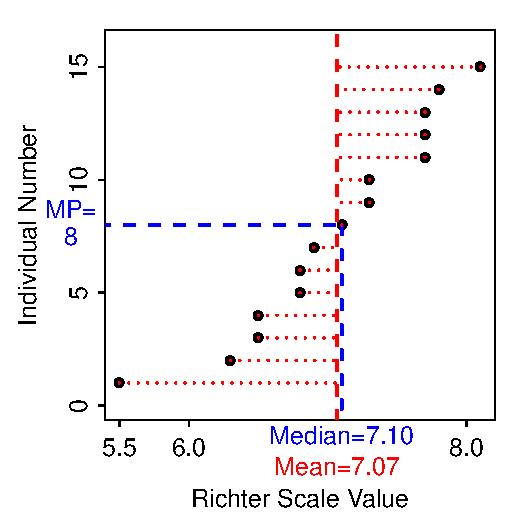
\includegraphics[width=.45\linewidth]{Figs/MeanMedianComp1-1} 
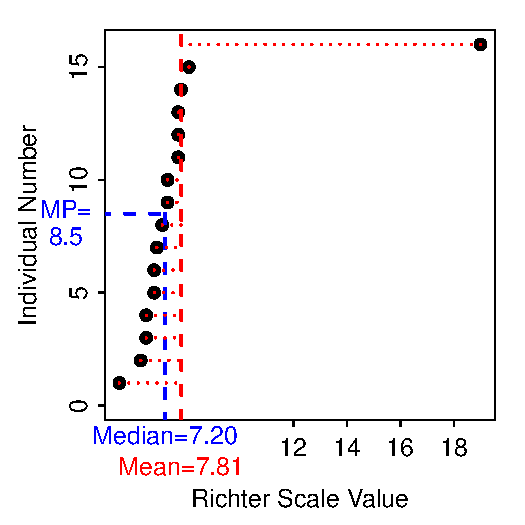
\includegraphics[width=.45\linewidth]{Figs/MeanMedianComp1-2} 

}

\caption[Plot of the individual number versus Richter scale values for the original earthquake data (\textbf{Left}) and the earthquake data with an extreme outlier (\textbf{Right})]{Plot of the individual number versus Richter scale values for the original earthquake data (\textbf{Left}) and the earthquake data with an extreme outlier (\textbf{Right}).  The median value is shown as a blue vertical line and the mean value is shown as a red vertical line.  Differences between each individual value and the mean value are shown with horizontal red lines.}\label{fig:MeanMedianComp1}
\end{figure}


\end{knitrout}

\warn{The mean balances the distance to individuals above and below the mean. The median balances the number of individuals above and below the median.}

\vspace{-12pt}
\warn{The sum of all differences between individual values and the mean (as properly calculated) equals zero.}

The mean and median differ in their sensitivity to outliers (\figref{fig:MeanMedianComp1}-Right).\index{Mean!Sensitivity to outliers}\index{Median!Sensitivity to outliers}  For example, suppose that an incredible earthquake with a Richter Scale value of 19.0 was added to the earthquake data set.  With this additional individual, the median increases from 7.1 to 7.2, but the mean increases from 7.1 to 7.8.  The outlier affects the value of the mean more than it affects the value of the median because of the way that each statistic measures center.  The mean will be pulled towards an outlier because it must ``put'' many values on the ``side'' of the mean away from the outlier so that the sum of the differences to the larger values and the sum of the differences to the smaller values will be equal.  Thus, the outlier in this example creates a large difference to the right of the mean so the mean has to ``move'' to the right to make this difference smaller, move more individuals to the left side of the mean, and increase the differences of individuals to the left of the mean to balance this one large individual.  The median on the other hand will simply ``put'' one more individual on the side opposite of the outlier because it balances the number of individuals on each side of it.  Thus, the median has to move very little to the right to accomplish this balance.

\warn{The mean is more sensitive (i.e., changes more) to outliers than the median; it will be ``pulled'' towards the outlier more than the median.}

The shape of the distribution, even if outliers are not present, also has an effect on the values of the mean and median as depicted in \figref{fig:MeanMedianShape}.  If a distribution is perfectly symmetric, then the median and mean (along with the mode) will be identical.  If the distribution is approximately symmetric, then the median and mean will be approximately equal.  If the distribution is right-skewed, then the mean will be greater than the median.  Finally, if the distribution is left-skewed, then the mean will be less than the median.

\begin{knitrout}
\definecolor{shadecolor}{rgb}{0.922, 0.922, 0.922}\color{fgcolor}\begin{figure}[hbtp]

{\centering 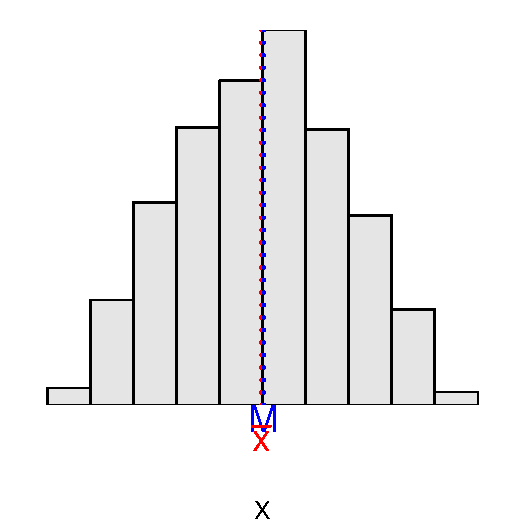
\includegraphics[width=.3\linewidth]{Figs/MeanMedianShape-1} 
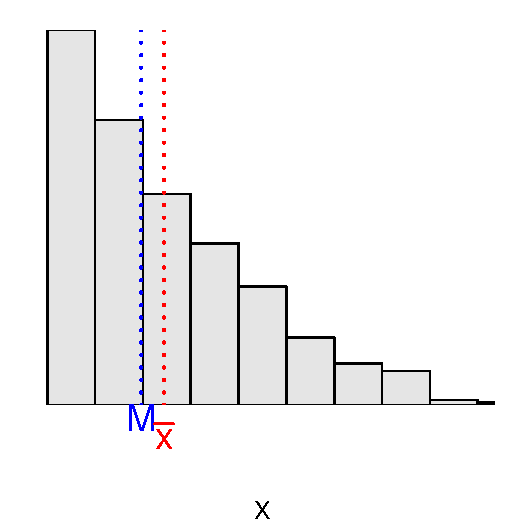
\includegraphics[width=.3\linewidth]{Figs/MeanMedianShape-2} 
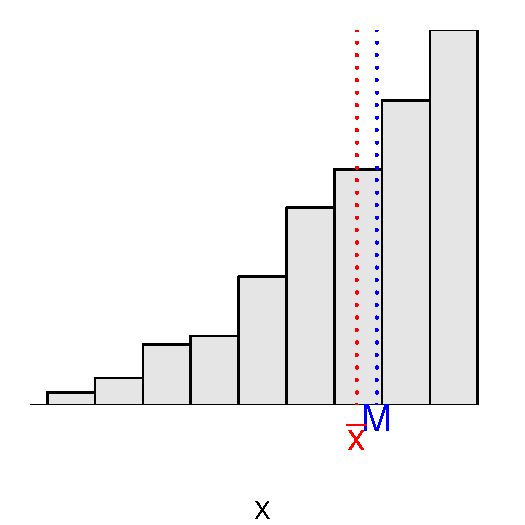
\includegraphics[width=.3\linewidth]{Figs/MeanMedianShape-3} 

}

\caption[Three differently shaped histograms with vertical lines superimposed at the median (M]{Three differently shaped histograms with vertical lines superimposed at the median (M; blue lines) and the mean ($\bar{x}$; red lines).}\label{fig:MeanMedianShape}
\end{figure}


\end{knitrout}

\warn{The mean and median are equal for symmetric distributions.}

\vspace{-12pt}
\warn{The mean is pulled towards the long tail of a skewed distribution. Thus, the mean is greater than the median for right-skewed distributions and the mean is less than the median for left-skewed distributions.}

As shown above, the mean and median measure center in different ways.  The question now becomes ``which measure of center is better?''  The median is a ``better'' measure of center when outliers are present.  In addition, the median gives a better measure of a typical individual when the data are skewed.  Thus, in this course, the median is used when outliers are present or the distribution of the data is skewed.\index{Median!When to use}  If the distribution is symmetric, then the purpose of the analysis will dictate which measure of center is ``better.''  However, in this course, use the mean when the data are symmetric or, at least, not strongly skewed.\index{Mean!When to use}

\warn{Describe center with the median if outliers are present or the data are skewed; use the mean if the data are symmetric and no outliers are present.}

\vspace{-12pt}
\begin{exsection}
  \item \label{revex:quEDALSkewMM}Is the mean less than, approximately equal to, or greater than the median for the distribution shown in Exercise \ref{revex:quEDALSkewg}? \ansref{ans:quEDALSkewMM}
  \item \label{revex:quEDAAsymMM}Is the mean less than, approximately equal to, or greater than the median for the distribution shown in Exercise \ref{revex:quEDASymg}? \ansref{ans:quEDAAsymMM}
  \item \label{revex:quEDARSkewMM}Is the mean less than, approximately equal to, or greater than the median for the distribution shown in Exercise \ref{revex:quEDARSkewg}? \ansref{ans:quEDARSkewMM}
  \item \label{revex:quEDARatio} Is the mean divided by the median less than 1, equal to 1, or greater than 1 for a symmetric distribution? \ansref{ans:quEDARatio}
  \item \label{revex:quEDABruleMM} From your calculation of the mean and median in Review Exercise  \ref{revex:quEDABrule} do you expect the histogram to be left-skewed, approximately symmetric, or right-skewed? \ansref{ans:quEDABruleMM}
  \item \label{revex:quEDAWIcMM} From your calculation of the mean and median in Review Exercise \ref{revex:quEDAWIc} do you expect the histogram to be left-skewed, approximately symmetric, or right-skewed? \ansref{ans:quEDAWIcMM}
\end{exsection}


\vspace{-18pt}
\section{Measures of Dispersion}
\vspace{-12pt}
There are three common measures of the dispersion of a distribution: the range, inter-quartile range (IQR), and standard deviation.\index{Dispersion}  The standard deviation is the most widely used.  The choice of which method to use depends, however, on what statistic you chose as the measure of center (which, as described in \sectref{sect:MeanMedian}, depends on the shape of the distribution, presence of outliers, and your purpose).

The range, IQR, and standard deviation computed in this section are summary statistics -- i.e., they are computations from individuals in a sample.  Thus, they should all be preceded with ``sample.''  See \sectref{sect:IVPPSS} for clarification on the differences between populations and samples and parameters and statistics.

\warn{Three measures of the dispersion of a distribution are the range, inter-quartile range (IQR), and standard deviation.}

\vspace{-12pt}
\warn{Measures of dispersion computed from individuals in a sample are preceded by ``sample''; those computed from all individuals in a population are preceded by ``population.''}

\subsection{Range}
The range is the difference between the maximum and minimum values in the data and measures the ultimate dispersion or spread of the data.\index{Range} The range in the mouse consumption data \tabrefp{tab:MouseData} is 18.4-9.4 = 9.0.

The range should never be used by itself as a measure of dispersion.  The range is extremely sensitive to outliers and is best used only to show all possible values present in the data.  The range (as strictly defined) also suffers from a lack of information.  For example, what does a range of 9 mean?  It can have a completely different interpretation if it came from values of 1 to 10 or if it came from values of 1000 to 1009.  Thus, the range is more instructive if presented as both the maximum and minimum value rather than the difference.

\defn{Range}{The difference between the maximum and minimum value in a data set.}

\vspace{-12pt}
\warn{Never use the range by itself as a measure of dispersion.}

\subsection{IQR}
Quartiles are the values for the three individuals that divide ordered data into four (approximately) equal parts.\index{Quartile}  Finding the three quartiles consists of finding the median, splitting the data into two equal parts at the median, and then finding the medians of the two halves.\footnote{You should review how a median is computed before proceeding with this section.}  A concern in this process is that the median is NOT part of either half if there is an odd number of individuals.  These steps are summarized as,
\begin{Enumerate}
  \item Order the data from smallest to largest.
  \item Find the median -- this is the second quartile (Q2).
  \item Split the data into two halves at the median.  If $n$ is odd (so that the median is one of the observed values), then the median is not part of either half.\footnote{Some authors put the median into both halves when $n$ is odd.  The difference between the two methods is minimal for large $n$.}
  \item Find the median of the lower half of data -- this is the 1st quartile (Q1).
  \item Find the median of the upper half of data -- this is the third quartile (Q3).
\end{Enumerate}

These calculations are illustrated with the earthquake data \tabrefp{tab:EQData}.  Recall from above \sectrefp{sec:Median} that the median (=7.1) is in the eighth position of the ordered data.  The value in the eighth position will not be included in either half.  Thus, the two halves of the data are 5.5 6.3 6.5 6.5 6.8 6.8 6.9 and 7.3 7.3 7.7 7.7 7.7 7.8 8.1.  Each half contains seven individuals, so the middle position for each half is $mp=\frac{7+1}{2}=4$.  Thus, the median for each half is the individual in the fourth position.  Therefore, the median of the first half is $Q1=6.5$ and the median of the second half is $Q3=7.7$.

As another example, consider the quartiles of the mouse consumption data (the median was computed in \sectref{sec:Median}).  Because $n=30$ is even, the halves of the data split naturally with 15 individuals in each half.  Therefore, the $mp=\frac{15+1}{2}=8$ and the median of each half is the value of the individual in the eighth position.  Thus, $Q1=12.5$ and $Q3=15.8$.  In summary, the first, second, and third quartiles for the mouse water consumption data are 12.5, 13.85, and 15.8, respectively.  These three values separate the ordered individuals into approximately four equally-sized groups -- those with values less than 12.5, with values between 12.5 and 13.85, with values between 13.85 and 15.8, and with values greater than 15.8.

\defn{Quartiles}{The values that divide the ordered data into quarters.}

The interquartile range is the difference between the third quartile (Q3) and the first quartile (Q1), namely Q3-Q1.\index{IQR!Calculation}  The IQR for the mouse consumption data is, thus, 15.8-12.5 = 3.3.  Intuitively, the IQR can be thought of as the ``range of the middle half of the data.''  The IQR is favored over the range because it is not sensitive to outliers (\textit{you should convince yourself that this is true}).  As with the range, however, the IQR suffers from a lack of information.  Thus, you should always present the IQR by presenting both Q1 and Q3 rather than the difference between the two.  Finally, the IQR should be chosen as the measure of dispersion when the median is used as the measure of center because they are conceptually related (both rely on position rather than actual value).  Thus, the IQR is used if outliers are present or the data are skewed.\index{IQR!When to use}

\defn{Inter-Quartile Range (IQR)}{The difference between the  third (Q3) and first (Q1) quartiles.}

\vspace{-12pt}
\warn{The IQR should be used as the measure of dispersion only if the median is chosen as the measure of center.}

\subsection{Standard Deviation}\label{sect:StdDev}
The sample standard deviation, denoted by $s$, can be thought of as ``the average difference between the observed values and the mean.''\footnote{This statement is not strictly correct as will become obvious.  However, this is an acceptable general interpretation of $s$.}\index{Standard Deviation!Sample symbol}\index{Standard Deviation!Interpretation}\index{Standard Deviation!Calculation}\index{Variance!Calculation}  The standard deviation is computed with these six steps:
\begin{Enumerate}
  \item Compute the sample mean (i.e., $\bar{x}$).
  \item For each value ($x_{i}$), find the difference between the value and the mean, namely $x_{i}-\bar{x}$.
  \item Square each difference, namely $(x_{i}-\bar{x})^{2}$.
  \item Add together all the squared differences.
  \item Divide this sum by $n-1$.  [\textit{Stopping here gives the sample variance, $s^{2}$.}]
  \item Square root the result from the previous step to get $s$.
\end{Enumerate}
These steps are neatly summarized with
\begin{equation}
  \label{eqn:SampleSD}
     s = \sqrt{\frac{\Sum_{i=1}^{n}(x_{i}-\bar{x})^{2}}{n-1}}
\end{equation}

The calculation of the standard deviation of the earthquake data \tabrefp{tab:EQData} is facilitated with the calculations shown in \tabref{tab:SDCalc}.  In \tabref{tab:SDCalc}, note that $\bar{x}$ is equal to the sum of the ``Value'' column divided by $n=15$ (i.e., $\bar{x}=7.07$).  The ``Diff'' column which contains each observed value minus the calculated $\bar{x}$ (i.e., Step 2).  The ``Diff$^2$'' column contains the square of the previously calculated differences (i.e., Step 3).  The sum of the ``Diff$^2$'' column is Step 4.  The sample variance (i.e., Step 5) is equal to this sum divided by $n-1=14$ or $\frac{6.773}{14}=0.484$.  Finally, the sample standard deviation is the square root of the sample variance or $s=\sqrt{0.484}=0.696$.  Thus, on average, each earthquake is approximately 0.7 Richter Scale units different than the average earthquake in these data.

\begin{table}[htbp]
  \caption{Table showing an efficient calculation of the standard deviation of the earthquake data.}
  \label{tab:SDCalc}
    \centering
    \begin{tabular}{cccc}
\hline\hline
Indiv & Value & Diff & Diff$^2$ \\
i & $x_{i}$ & $x_{i}-\bar{x}$ & $(x_{i}-\bar{x})^{2}$ \\
\hline
1 & 5.5 & -1.57 & 2.454 \\
2 & 6.3 & -0.77 & 0.588 \\
3 & 6.5 & -0.57 & 0.321 \\
4 & 6.5 & -0.57 & 0.321 \\
5 & 6.8 & -0.27 & 0.071 \\
6 & 6.8 & -0.27 & 0.071 \\
7 & 6.9 & -0.17 & 0.028 \\
8 & 7.1 & 0.03 & 0.001 \\
9 & 7.3 & 0.23 & 0.054 \\
10 & 7.3 & 0.23 & 0.054 \\
11 & 7.7 & 0.63 & 0.401 \\
12 & 7.7 & 0.63 & 0.401 \\
13 & 7.7 & 0.63 & 0.401 \\
14 & 7,8 & 0.73 & 0.538 \\
15 & 8.1 & 1.03 & 1.068 \\
\hline
Sum & 106 & 0 & 6.773 \\
\hline\hline
    \end{tabular}
\end{table}

\defn{Standard Deviation}{``Essentially'' the average deviation or difference of individuals from the mean.}

\vspace{-12pt}
\warn{In the standard deviation calculations don't forget to take the square root of the variance.}

There are three characteristics of the standard deviation that you should be aware of:\index{Standard Deviation!Characteristics}
\vspace{-12pt}
\begin{Enumerate}
  \item $s \geq$ 0 ($s$=0 only if there is no dispersion; i.e., all values are the same).
  \item $s$ is strongly influenced by outliers.
  \item $s$ is inflated for skewed distributions (similar to the mean).
\end{Enumerate}
\vspace{-12pt}
The final two characteristics are a result of the standard deviation being computed from the \textbf{values}, rather than the position, of the individuals (as is the mean).  The argument here is the same as it was for the mean.  In fact, it should be obvious that the mean and standard deviation are conceptually linked (i.e., they both require the actual values and the mean is within the standard deviation calculation).

\warn{The standard deviation should be used as the measure of dispersion only if the mean is chosen as the measure of center.}

At the beginning of this section, the standard deviation was defined as ``essentially the average difference between the values and the mean.''\index{Standard Deviation!Interpretation} \textbf{Essentially} was emphasized because the formula for the standard deviation does not simply add together the differences and divide by $n$ as this definition would imply.  Notice in \tabref{tab:SDCalc} that the sum of the differences from the mean is 0.  This will be the case for all standard deviation calculations using the correct mean, because the mean balances the distance to individuals below the mean with the distance of individuals above the mean (review \sectref{sect:MeanMedian}).  Thus, the mean difference will always be zero.  This ``problem'' is corrected by squaring the differences before summing them.  To get back to the original units, the squaring is later ``reversed'' by the square root.  So, more accurately, the standard deviation is the square root of the average squared difference between the values and the mean.  Therefore, the original definition of the standard deviation is strictly incorrect; however, it works well as a practical definition of the meaning of the standard deviation.

\warn{Use the fact that the sum of all differences from the mean equals zero as a check of your standard deviation calculation.}

Further note that the mean is the value that minimizes the value of the standard deviation calculation -- i.e., putting any other value besides the mean into the standard deviation equation will result in a larger value.

Finally, why is the sum of the squared differences divided by $n-1$, rather than $n$, in the standard deviation calculation?  Recall (from \sectref{sect:IVPPSS}) that statistics are meant to estimate parameters.  The sample standard deviation is supposed to estimate the population standard deviation ($\sigma$).  Theorists have shown that if we divide by $n$, $s$ will consistently underestimate $\sigma$.  Thus, $s$ calculated in this way would be a biased estimator of $\sigma$.  Theorists have found, though, that dividing by $n-1$ will cause $s$ to be an unbiased estimator of $\sigma$.  Being unbiased is generally good -- it means that on average our statistic estimates our parameter (this concept is discussed in more detail in \modref{chap:SamplingDist}).

\vspace{-6pt}
\subsection{Measures of Dispersion in R} \label{sect:DescStatsDispersion}\index{Standard Deviation!Calculation}\index{IQR!Calculation}\index{Quartile!Calculation}\index{Range!Calculation}
\vspace{-10pt}
The minimum, maximum, Q1, Q3, and standard deviation are calculated with \R{Summarize()} as described previously for the mean and median. Thus, $s=$21.59, the IQR is from $Q1=$97.00 to $Q3=$118.00, and the range is from 48.00 to 146.00.
\begin{knitrout}
\definecolor{shadecolor}{rgb}{0.922, 0.922, 0.922}\color{fgcolor}\begin{kframe}
\begin{verbatim}
> Summarize(~days,data=LSI,digits=2)
     n nvalid   mean     sd    min     Q1 median     Q3    max 
 42.00  39.00 107.85  21.59  48.00  97.00 114.00 118.00 146.00 
\end{verbatim}
\end{kframe}
\end{knitrout}

\vspace{-8pt}
\begin{exsection}
  \item \label{revex:quEDABruleDisp} \rhw{} Compute the range, IQR, and standard deviation for the maximum gauge heights of the Bois Brule River in Brule, WI from Exercise \ref{revex:quEDABrule} both ``by hand'' and with R. \ansref{ans:quEDABruleDisp}

  \item \label{revex:quEDAWIDisp} \rhw{} Compute the range, IQR, and standard deviation for the population density of Wisconsin counties from Exercise \ref{revex:quEDAWIc} both ``by hand'' and with R. \ansref{ans:quEDAWIDisp}

  \item \label{revex:quEDACreatPhosph3} \rhw{} Compute the range, IQR, and standard deviation of the creatine phosphate data in Exercise \ref{revex:quEDACreatPhosph}. \ansref{ans:quEDACreatPhosph3}

  \item \label{revex:quEDAAirPolln3} \rhw{} \hspace{12pt} Compute the range, IQR, and standard deviation of the CO data in Exercise \ref{revex:quEDAAirPolln}. \ansref{ans:quEDAAirPolln3}
\end{exsection}


\section{Overall Summaries}
Overall numerical summaries come from considering the relationship between measures of center and dispersion.  From the previous section it was seen that the standard deviation and mean are conceptually linked, as are the median and IQR.  Indeed, the linked measure of center must be computed first in both dispersion calculations.  Thus, if the mean is used to measure center, then the standard deviation must be used to measure dispersion.\index{Standard Deviation!When to use}  Similarly, if the median is used to measure center, then the IQR must be used to measure dispersion.\footnote{Recall that the range will never be used by itself.}\index{IQR!When to use}

\subsection{Boxplots}
The median, range, and IQR form the \textbf{five-number summary}.\index{Five Number Summary}  Specifically, the five-number summary consists of the minimum value, Q1, median, Q3, and maximum value.  The five-number summary for the mouse consumption data is 48.0, 97.0, 114.0, 118.0, and 146.0 (all values computed in the previous section).

The five-number summary may be displayed as a \textbf{boxplot}.\index{Boxplot!Construction}  A traditional boxplot \figrefp{fig:MouseBoxplot} consists of a horizontal line at the median, horizontal lines at Q1 and Q3 that are connected with vertical lines to form a box, and vertical lines from Q1 to the minimum value and from Q3 to the maximum value.  The vertical lines have been modified on modern boxplots to allow easier detection of outliers. Specifically, the upper line extends from Q3 to the last observed value that is within 1.5 IQRs of Q3 and the lower line extends from Q1 to the last observed value that is within 1.5 IQRs of Q1.  Observed values outside of the whiskers are termed ``outliers'' by this algorithm and are typically plotted with circles or asterisks.  If no individuals are deemed ``outliers'' by this algorithm, then the two traditional and modern boxplots will be the same.

\begin{knitrout}
\definecolor{shadecolor}{rgb}{0.922, 0.922, 0.922}\color{fgcolor}\begin{figure}[hbtp]

{\centering 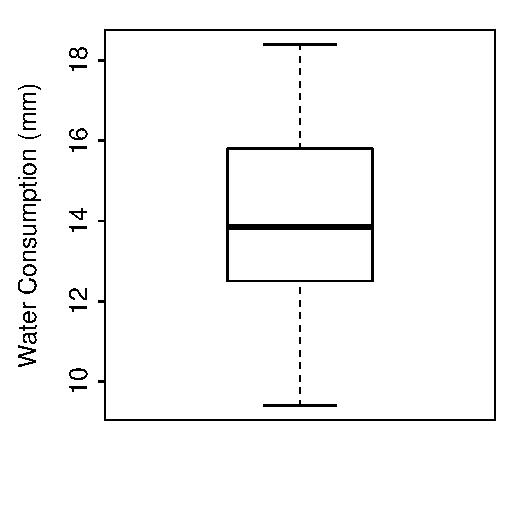
\includegraphics[width=.4\linewidth]{Figs/MouseBoxplot-1} 

}

\caption[Boxplot of the mouse consumption data]{Boxplot of the mouse consumption data.}\label{fig:MouseBoxplot}
\end{figure}


\end{knitrout}

\defn{Boxplot}{Generally, a graphical depiction of the five-number summary.}

The relative length from the median to Q1 and the median to Q3 (i.e., the position of the median line in the box) indicates the shape of the distribution.\index{Boxplot!Interpretation}  If the distribution is left-skewed (i.e., lesser-valued individuals are ``spread out''; \figref{fig:BoxplotShape}-Right), then median-Q1 will be greater than Q3-median.  In contrast, if the distribution is right-skewed (i.e., larger-valued individuals are spread out; \figref{fig:BoxplotShape}-Middle), then Q3-median will be greater than median-Q1.  Thus, if the distribution is right-skewed then the median will be closer to Q1 than to Q3, if the distribution is left-skewed then the median will be closer to Q3 than to Q1, and if the distribution is approximately symmetric (\figref{fig:BoxplotShape}-Left) then the median will be in the middle of the box.

\begin{knitrout}
\definecolor{shadecolor}{rgb}{0.922, 0.922, 0.922}\color{fgcolor}\begin{figure}[hbtp]

{\centering 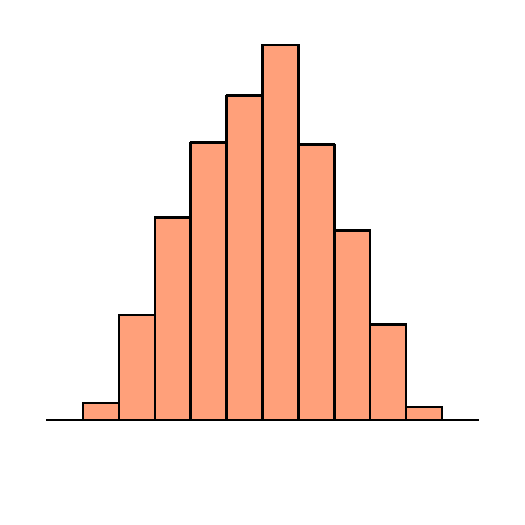
\includegraphics[width=.3\linewidth]{Figs/BoxplotShape-1} 
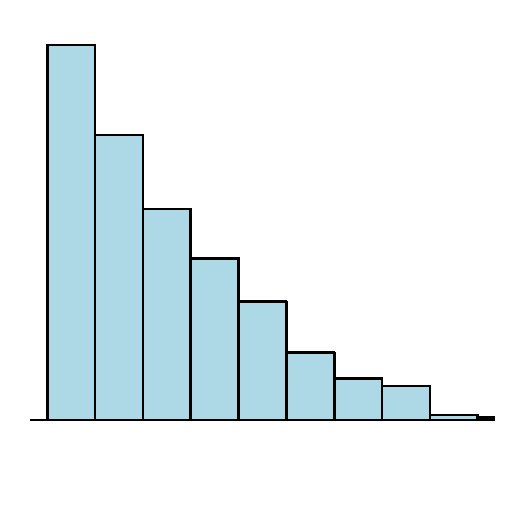
\includegraphics[width=.3\linewidth]{Figs/BoxplotShape-2} 
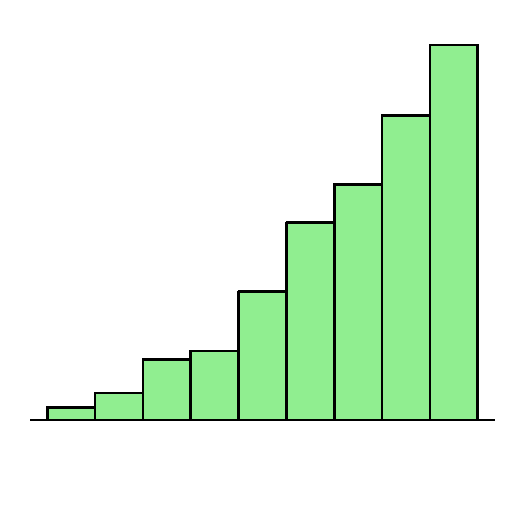
\includegraphics[width=.3\linewidth]{Figs/BoxplotShape-3} 
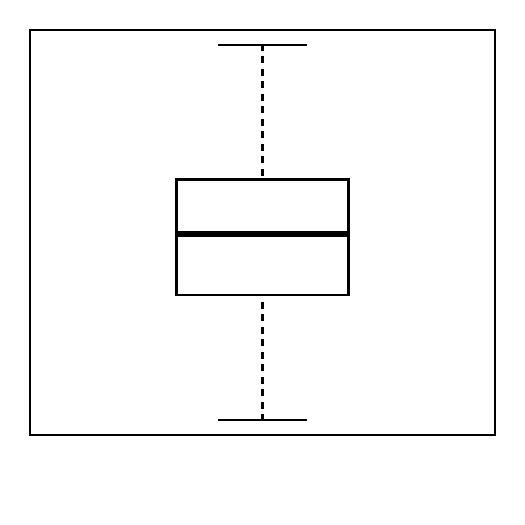
\includegraphics[width=.3\linewidth]{Figs/BoxplotShape-4} 
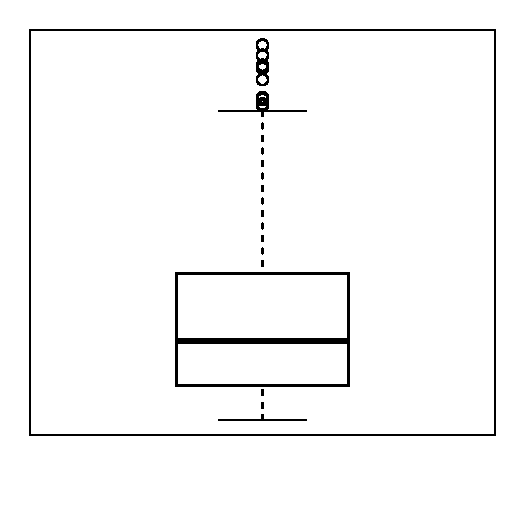
\includegraphics[width=.3\linewidth]{Figs/BoxplotShape-5} 
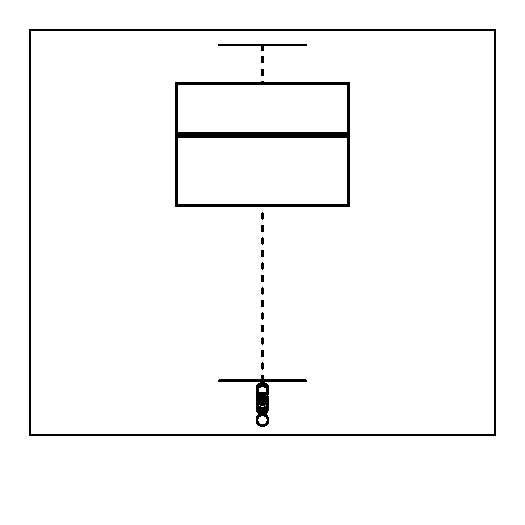
\includegraphics[width=.3\linewidth]{Figs/BoxplotShape-6} 

}

\caption[Histograms and boxplots for several different shapes of distributions]{Histograms and boxplots for several different shapes of distributions.}\label{fig:BoxplotShape}
\end{figure}


\end{knitrout}

\warn{If a distribution is right-skewed, then the median will be closer to Q1 than to Q3. If the distribution is left-skewed, then the median will be closer to Q3 than to Q1.}

\vspace{-12pt}
\warn{Even though shape can be described from a boxplot, it is always easier to describe shape from a histogram.}

A boxplot is constructed in R with \R{boxplot()}.  This function requires only the name of the quantitative variable as the first argument although the x- and y-axes are labeled with \R{xlab=} and \R{ylab=}, respectively.

\newpage
\begin{exsection}
  \item \label{revex:quEDABrule5N} What is the five-number summary for the maximum gauge heights of the Bois Brule River in Brule, WI from Exercise \ref{revex:quEDABrule}. \ansref{ans:quEDABrule5N}
  \item \label{revex:quEDAWI5N} \rhw{} Construct a boxplot for the population density of Wisconsin counties from Exercise \ref{revex:quEDAWIc}. \ansref{ans:quEDAWI5N}
  \item \label{revex:quEDABoxLeft} What is the shape of the left boxplot below? \ansref{ans:quEDABoxLeft}

\begin{center}
  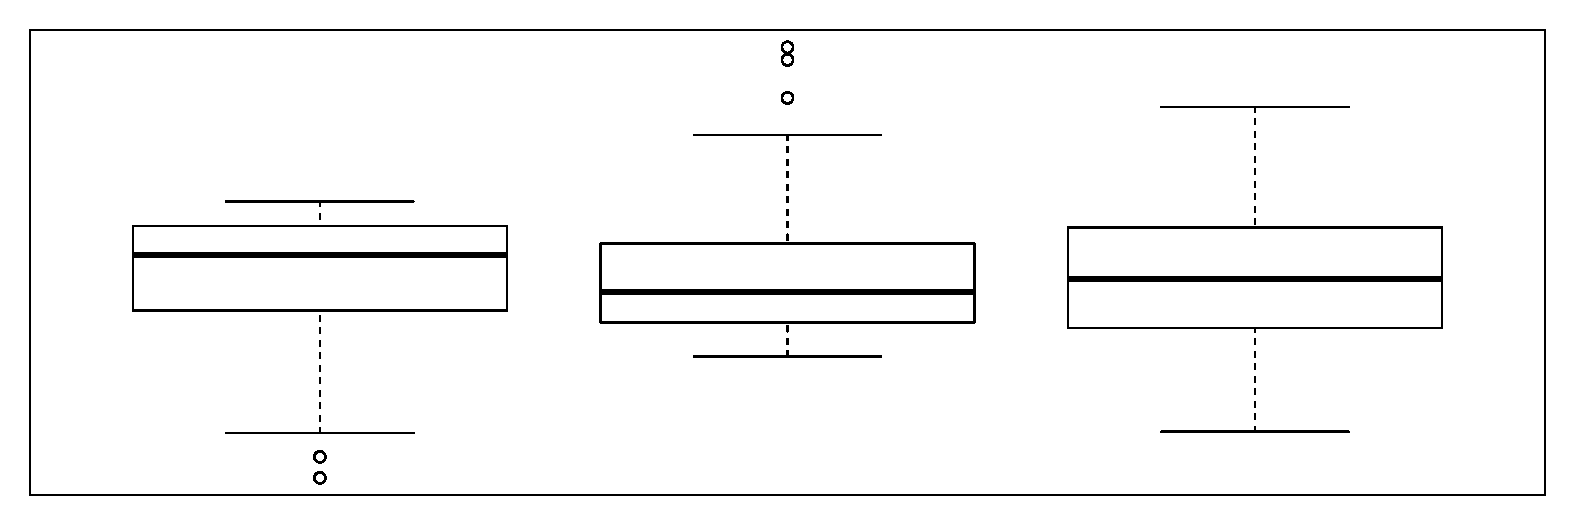
\includegraphics[width=4in]{Figs/BoxplotQuest-1}
\end{center}

  \item \label{revex:quEDABoxRight} What is the shape of the middle boxplot above? \ansref{ans:quEDABoxRight}
  \item \label{revex:quEDABoxSym} What is the shape of the right boxplot above? \ansref{ans:quEDABoxSym}
  \item \label{revex:quEDALSkewCtr} If the distribution is skewed left, which measure should you generally use to measure center? \ansref{ans:quEDALSkewCtr}
  \item \label{revex:quEDARSkewCtr} Which measure of center should you generally use for a right-skewed distribution? \ansref{ans:quEDARSkewCtr}
  \item \label{revex:quEDASymCtr} Which measure of center should you generally use for a symmetric distribution? \ansref{ans:quEDASymCtr}
  \item \label{revex:quEDASymDisp} Which measure of dispersion should you generally use for a symmetric distribution? \ansref{ans:quEDASymDisp}
  \item \label{revex:quEDALSkewDisp} Which measure of dispersion should you generally use for a left-skewed distribution? \ansref{ans:quEDALSkewDisp}
  \item \label{revex:quEDARSkewDisp} Which measure of dispersion should you generally use for a right-skewed distribution? \ansref{ans:quEDARSkewDisp}
  \item \label{revex:quEDAQShape1} Is Q3-Q2 less than, approximately equal to, or greater than Q2-Q1 if the data are left-skewed? \ansref{ans:quEDAQShape1}
  \item \label{revex:quEDAQShape2} What is the shape of the distribution if Q3-Q2 is greater than Q2-Q1? \ansref{ans:quEDAQShape2}
\end{exsection}

\section{Multiple Groups} \label{sect:MultGroups}
It is common to conduct a univariate EDA for a quantitative variable separately for groups of individuals.  In these cases it is beneficial to have a function that will efficiently construct a histogram and compute summary statistics for the quantitative variable separated by the levels of a factor variable.  Separate histograms are constructed with \R{hist()} if the first argument is a ``formula'' of the type \R{quant\TILDE group} where \R{quant} represents the quantitative response variable of interest and \R{group} represents the factor variable that indicates to which group the individual belongs.\index{Histogram!Multiple}  The data frame that contains \R{quant} and \R{group} is given to \R{data=}.  Summary statistics are separated by group by supplying the same formula and \R{data=} arguments to \R{Summarize()}.

As an example, suppose that you want to examine the average annual days of ice for each decade (using the \R{LSI} data).  One might expect to use the \R{days\TILDE decade} formula except that the \R{decade} variable is not a factor.\footnote{It was not a factor because the data in \R{decade} looks numeric to R.}  This can be connverted to a factor by including the variable to the left of the assignment operator and in \R{factor()}. The desired grouping variable may already be a factor in many data.frames and, thus, will not require modification with \R{factor()}.
\begin{knitrout}
\definecolor{shadecolor}{rgb}{0.922, 0.922, 0.922}\color{fgcolor}\begin{kframe}
\begin{verbatim}
> LSI$decade <- factor(LSI$decade)
> str(LSI)
'data.frame':	42 obs. of  4 variables:
 $ season: int  1955 1956 1957 1958 1959 1960 1961 1962 1963 1964 ...
 $ decade: Factor w/ 5 levels "1950","1960",..: 1 1 1 1 1 2 2 2 2 2 ...
 $ temp  : num  22.9 23 25.7 20 24.8 ...
 $ days  : int  87 137 106 97 105 118 118 136 91 NA ...
\end{verbatim}
\end{kframe}
\end{knitrout}

Histograms \figrefp{fig:mhist1} and summary statistics separated by decade are then constructed as below.
\begin{knitrout}
\definecolor{shadecolor}{rgb}{0.922, 0.922, 0.922}\color{fgcolor}\begin{kframe}
\begin{verbatim}
> hist(days~decade,data=LSI,ylab="Days of Ice Cover",w=20)
> Summarize(days~decade,data=LSI,digits=2)
  decade  n nvalid   mean    sd min     Q1 median    Q3 max
1   1950  5      5 106.40 18.73  87  97.00  105.0 106.0 137
2   1960 10      8 113.12 14.80  91 104.20  116.0 119.8 136
3   1970 10     10 115.50 19.19  82 105.80  115.0 124.0 146
4   1980 10     10 103.80 24.88  48  90.25  116.0 118.0 123
5   1990  7      6  96.00 28.53  62  72.00  100.5 114.0 132
\end{verbatim}
\end{kframe}\begin{figure}[hbtp]

{\centering 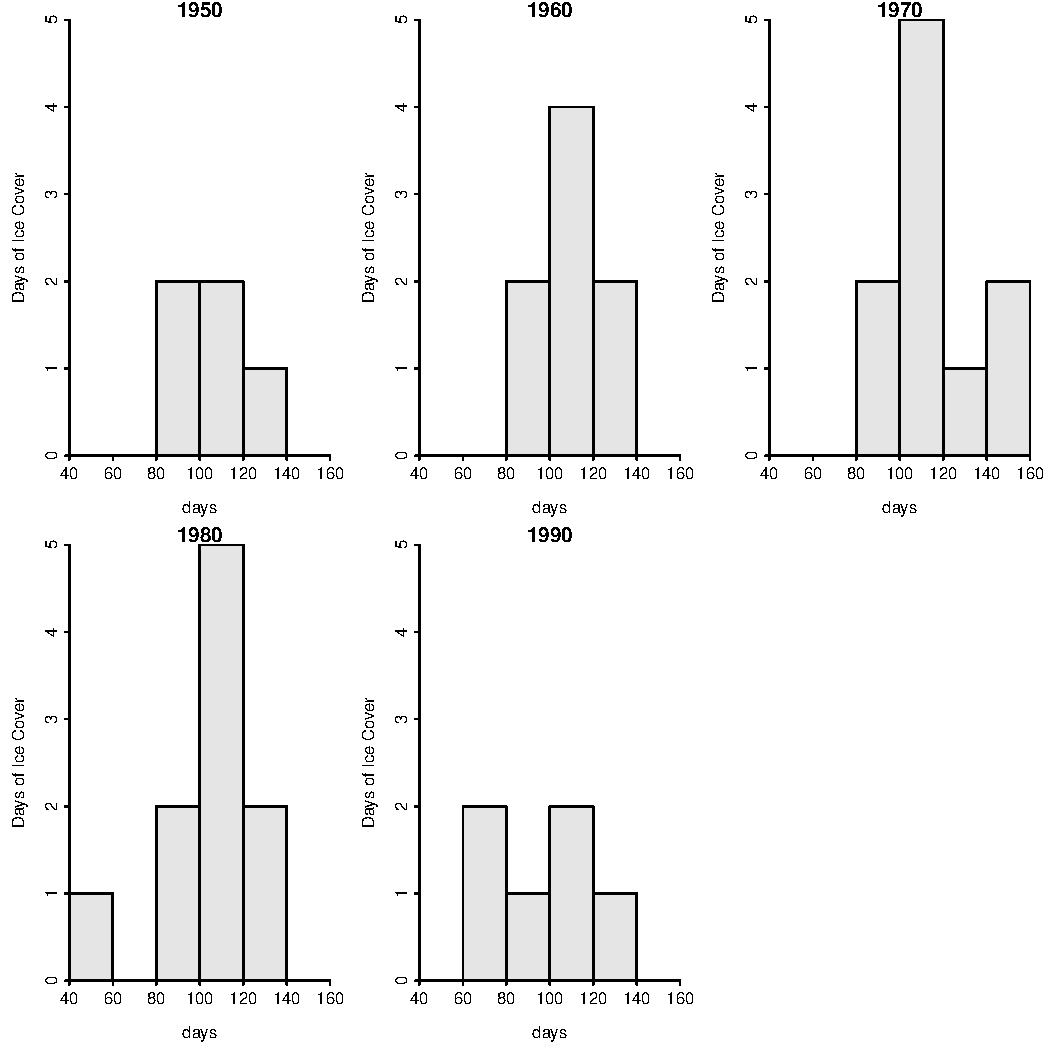
\includegraphics[width=.8\linewidth]{Figs/mhist1-1} 

}

\caption[Histograms of the duration of ice cover at ice gauge 9004 in Lake Superior by each decade]{Histograms of the duration of ice cover at ice gauge 9004 in Lake Superior by each decade.}\label{fig:mhist1}
\end{figure}


\end{knitrout}

Side-by-side boxplots \figrefp{fig:Boxplot1} are an alternative to separated histograms and are constructed by including the same formula and \R{data=} arguments to \R{boxplot()}.
\begin{knitrout}
\definecolor{shadecolor}{rgb}{0.922, 0.922, 0.922}\color{fgcolor}\begin{kframe}
\begin{verbatim}
> boxplot(days~decade,data=LSI,ylab="Days of Ice Cover",xlab="Decade")
\end{verbatim}
\end{kframe}\begin{figure}[hbtp]

{\centering 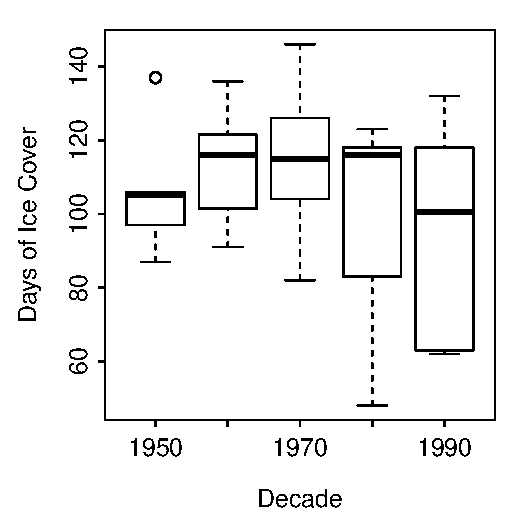
\includegraphics[width=.4\linewidth]{Figs/Boxplot1-1} 

}

\caption[Boxplot of the duration of ice cover at ice gauge 9004 in Lake Superior by each decade]{Boxplot of the duration of ice cover at ice gauge 9004 in Lake Superior by each decade.}\label{fig:Boxplot1}
\end{figure}


\end{knitrout}

\clearpage
\begin{exsection}
  \item \label{revex:EDAArsenic1} \rhw{} Arsenic concentrations were measured in the well water and in the toe nails of 21 people with home wells.  Also recorded were the person's age, sex, and qualitative measurements of usage for drinking and cooking.  The data are found in \href{https://raw.githubusercontent.com/droglenc/NCData/master/Arsenic.csv}{Arsenic.csv}.  Load these data into R to answer the questions below. \ansref{ans:EDAArsenic1}
  \begin{Enumerate}
    \item Construct a univariate EDA for the well water measurements.
    \item Construct a univariate EDA for the measurements of arsenic in the toe nails.
    \item Construct a univariate EDA for the toe nail arsenic levels separated by levels of drinking water usage.
  \end{Enumerate}
\end{exsection}


\section{Example Interpretations}\index{EDA!Univariate!Quantitative}
\vspace{-12pt}
While most of the previous sections focused on how to construct various graphs and numerical summaries, the most important aspect of this module is that you can make appropriate interpretations for an EDA from the summary results.  For quantitative data, an appropriate EDA consists of identifying the shape, center, dispersion, and outliers for the variable.  For categorical data, an appropriate EDA consists of identifying the major characteristics among the categories.  Below, I model properly constructed EDAs for the mouse consumption data and two new data sets.

\subsubsection{Mouse Consumption Example}
\vspace{-12pt}
\begin{quote}
\textit{Construct a proper EDA for the following situation and data -- `The  following measurements \tabrefp{tab:MouseData} are of the consumption of water in one hour by mice in a laboratory setting.'}
\end{quote}
\vspace{-12pt}


Mouse water consumption is approximately symmetric without any outliers present \figrefp{fig:MouseHist2}.  The center of the distribution is best measured by the mean, which is 14.05 ml \tabrefp{tab:MouseStats}.  The range of water consumption by the mice in the sample is from 9.4 to 18.4 ml while the dispersion as measured by the standard deviation is 2.41 ml \tabrefp{tab:MouseStats}.  I chose to use the mean and standard deviation because the data were symmetric with no outliers.  [\textit{NOTE: 1) use of units, 2) reference to the figure and table, 3) labeling of the figure and table, 4) median and IQR were not discussed as I chose to use the mean and standard deviation, 5) the range was not used alone as a measure of dispersion, 6) the explanation for why the mean and standard deviation were used rather than the median and IQR, and 7) R code was provided.}]

% latex table generated in R 3.3.3 by xtable 1.8-2 package
% Wed Apr 26 20:49:44 2017
\begin{table}[ht]
\centering
\caption{Descriptive statistics of mouse water consumption.} 
\label{tab:MouseStats}
\begin{tabular}{rrrrrrrr}
  \hline
n & mean & sd & min & Q1 & median & Q3 & max \\ 
  \hline
30.00 & 14.05 & 2.41 & 9.40 & 12.52 & 13.85 & 15.80 & 18.40 \\ 
   \hline
\end{tabular}
\end{table}


\begin{minipage}{\textwidth}
R Appendix:
\begin{knitrout}
\definecolor{shadecolor}{rgb}{0.922, 0.922, 0.922}\color{fgcolor}\begin{kframe}
\begin{verbatim}
setwd("c:/data/")
mc <- read.csv("MouseData.csv")
str(mc)
Summarize(~consump,data=mc,digits=2)
hist(~consump,data=mc,xlab="Water Consumption (mm)")
\end{verbatim}
\end{kframe}
\end{knitrout}
\end{minipage}

\subsubsection{Crayfish Temperature Selection}
\begin{quote}
\textit{\cite{Peck1985} examined the temperature selection of dominant and subdominant crayfish (\textit{Orconectes virilis}) together in an artificial stream.  The temperature ($^{o}$C) selection by the dominant crayfish in the presence of subdominant crayfish in these experiments was recorded below.  Thoroughly describe all aspects of the distribution of selected temperatures.}
\end{quote}

% latex table generated in R 3.3.3 by xtable 1.8-2 package
% Wed Apr 26 20:49:44 2017
\begin{tabular}{rrrrrrrrrrrrrrrr}
  30 & 26 & 26 & 26 & 25 & 25 & 25 & 25 & 25 & 24 & 24 & 24 & 24 & 24 & 24 & 23 \\ 
  23 & 23 & 23 & 22 & 22 & 22 & 22 & 21 & 21 & 21 & 20 & 20 & 19 & 19 & 18 & 16 \\ 
  \end{tabular}


The shape of temperatures selected by the dominant crayfish is slightly left-skewed \figrefp{fig:CrayfishTempHist} with a possible weak outlier at the maximum value of 30$^{o}$C \tabrefp{tab:CrayfishTempStats}.  The center is best measured by the median, which is 23$^{o}$C \tabrefp{tab:CrayfishTempStats} and the dispersion is best measured by the IQR, which is from 21 to 25$^{o}$C \tabrefp{tab:CrayfishTempStats}.  I used the median and IQR because of the (combined) skewed shape and outlier present.

\begin{knitrout}
\definecolor{shadecolor}{rgb}{0.922, 0.922, 0.922}\color{fgcolor}\begin{figure}[hbtp]

{\centering 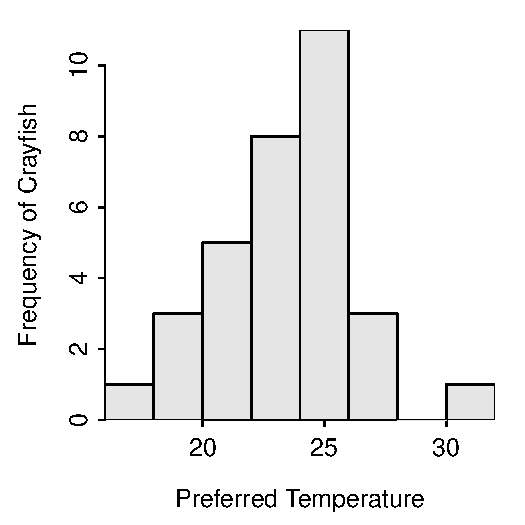
\includegraphics[width=.4\linewidth]{Figs/CrayfishTempHist-1} 

}

\caption[Histogram of crayfish temperature preferences]{Histogram of crayfish temperature preferences.}\label{fig:CrayfishTempHist}
\end{figure}


\end{knitrout}

% latex table generated in R 3.3.3 by xtable 1.8-2 package
% Wed Apr 26 20:49:44 2017
\begin{table}[ht]
\centering
\caption{Descriptive statistics of crayfish temperature preferences.} 
\label{tab:CrayfishTempStats}
\begin{tabular}{rrrrrrrr}
  \hline
n & mean & sd & min & Q1 & median & Q3 & max \\ 
  \hline
32.00 & 22.88 & 2.79 & 16.00 & 21.00 & 23.00 & 25.00 & 30.00 \\ 
   \hline
\end{tabular}
\end{table}


\begin{minipage}{\textwidth}
R Appendix:
\begin{knitrout}
\definecolor{shadecolor}{rgb}{0.922, 0.922, 0.922}\color{fgcolor}\begin{kframe}
\begin{verbatim}
setwd("c:/data/")
cray <- read.csv("Crayfish.csv")
str(cray)
hist(~temp,data=cray,xlab="Preferred Temperature",ylab="Frequency of Crayfish",w=2)
Summarize(~temp,data=cray,digits=2)
\end{verbatim}
\end{kframe}
\end{knitrout}
\end{minipage}

\newpage
\begin{exsection}
  \item \label{revex:quEDACP} \rhw{} Construct a proper EDA for the creatine phosphokinase data presented in Exercise \ref{revex:quEDACreatPhosph}.  Make sure to defend your choice of numerical summaries.  \ansref{ans:quEDACP}
  \item \label{revex:quEDADJTI} \rhw{} \hspace{12pt} The Dow Jones Travel Index tracks the cost of hotel and car-rental rates in 20 major cities.  For its May 7, 1996, survey the following rates were given for the 20 cities: 152, 180, 167, 119, 115, 113, 119, 135, 140, 126, 114, 133, 205, 104, 149, 124, 127, 161, 106, and 179.  Thoroughly describe the distribution of these data.  [\textit{Note: You can use fewer than the ideal number of bars on your histogram because the sample size is so small in this situation.}] \ansref{ans:quEDADJTI}
  \item \label{revex:quEDAZoo2} \rhw{} The data in \href{https://raw.githubusercontent.com/droglenc/NCData/master/Zoo2.csv}{Zoo2.csv} contains the physical size (in acres) of a sample of zoos from around the United States.  Perform a univariate EDA on the \var{size} variable. \ansref{ans:quEDAZoo2}
\end{exsection}



\chapter{Univariate EDA - Categorical} \label{chap:UnivEDACat}
\begin{ChapObj}{\boxwidth}
  \textbf{Objectives:}
  \begin{Enumerate}
    \item Construct frequency and percentage tables with categorical data.
    \item Construct bar-charts with categorical data, and
    \item Use tables and graphs to describe the categorical data.
  \end{Enumerate}
\end{ChapObj}

\minitoc
\vspace{24pt}

\lettrine{I}{nterpreting summaries of a} single categorical variable is more intuitive and less defined than that for quantitative data.\index{EDA!Univariate!Categorical}  Specifically, one DOES NOT describe shape, center, dispersion, and outliers for categorical data.  In this module, methods to construct tables and graphs for categorical data are described and the interpretation of the results demonstrated.  These concepts are illustrated with data recorded about MTH107 students in the Winter 2010 semester.  Whether or not a student was required to take the course for a subset of individuals is shown in \tabref{tab:MTH107Subset}.

\begin{table}[htbp]
  \caption{Whether (Y) or not (N) MTH107 was required for eight individuals in MTH107 in Winter 2010.}
  \label{tab:MTH107Subset}
  \centering
  \begin{Verbatim}[xleftmargin=10mm]
Individual  1  2  3  4  5  6  7  8
Required    Y  N  N  Y  Y  Y  N  Y
  \end{Verbatim}
\end{table}


\section{Summary Tables}
\vspace{-12pt}
A simple method to summarize categorical data is to count the number of individuals in each category (or level) of the categorical variable.  These counts are called frequencies and the resulting table \tabrefp{tab:MTH107SubsetFreq} is called a frequency table.\index{Table!Frequency}  From this table, it is seen that there were five students that were required and three that were not required to take MTH107.

\begin{table}[htbp]
  \caption{Frequency table for whether MTH107 was required (Y) or not (N) for eight individuals in MTH107 in Winter 2010.}
  \label{tab:MTH107SubsetFreq}
  \centering
  \begin{Verbatim}[xleftmargin=15mm]
Required  Freq
    Y       5
    N       3
  \end{Verbatim}
\end{table}

\vspace{-12pt}
\warn{Frequency tables show the number of individuals in each category of a categorical variable.}

The remainder of this module will use the results from the entire class rather than the subset used above.  For example, the frequency tables of individuals by sex and year-in-school for the entire class is in \tabref{tab:Mth107Freq}.

\begin{table}[htbp]
  \caption{Frequency tables for whether (Y) or not (N) MTH107 was required (Left) and year-in-school (Right) for all individuals in MTH107 in Winter 2010.}
  \label{tab:Mth107Freq}
  \centering
  \begin{Verbatim}[xleftmargin=15mm]
Required  Freq          Year  Freq
    Y      38            Fr    19
    N      30            So    12
                         Jr    29
                         Sr     9
   \end{Verbatim}
\end{table}

Frequency tables are often modified to show the percentage of individuals in each category.  These modified tables are called \textbf{percentage tables}.\index{Table!Percentage}  Percentage tables are constructed from frequency tables by dividing the number of individuals in each category by the total number of individuals examined ($n$) and then multiplying by 100.  For example, the percentage tables for both whether or not MTH107 was required and year-in-school \tabrefp{tab:Mth107Prop} for students in MTH107 is constructed from \tabref{tab:Mth107Freq} by dividing the value in each cell by 68, the total number of students in the class, and then multiplying by 100.  From this it is seen that 55.9\% of students were required to take the course and 13.2\% were seniors.

\begin{table}[htbp]
  \caption{Percentage tables for whether (Y) or not (N) MTH107 was required (Left) and year-in-school (Right) for all individuals in MTH107 in Winter 2000.}
  \label{tab:Mth107Prop}
  \centering
  \begin{Verbatim}[xleftmargin=5mm]
Required   Perc          Year   Perc
   Y       55.9           Fr    27.9
   N       44.1           So    17.6
                          Jr    42.6
                          Sr    13.2
  \end{Verbatim}
\end{table}

\vspace{-12pt}
\warn{Percentage tables show the percentage of all individuals in each category of a categorical variable.}

\subsection{Tables in R}
The General Sociological Survey (GSS) is a very large survey that has been administered 25 times since 1972.  The purpose of the GSS is to gather data on contemporary American society in order to monitor and explain trends in attitudes, behaviors, and attributes.  One question that was asked in a recent GSS was ``How often do you make a special effort to sort glass or cans or plastic or papers and so on for recycling?''  These data are found in the \var{recycle} variable in \href{https://raw.githubusercontent.com/droglenc/NCData/master/GSSEnviroQues.csv}{GSSEnviroQues.csv}.
\begin{knitrout}
\definecolor{shadecolor}{rgb}{0.922, 0.922, 0.922}\color{fgcolor}\begin{kframe}
\begin{verbatim}
> GSS <- read.csv("data/GSSEnviroQues.csv")
> str(GSS)
'data.frame':	3539 obs. of  2 variables:
 $ recycle: Factor w/ 5 levels "Always","Never",..: 1 1 1 1 1 1 1 1 1 1 ...
 $ tempgen: Factor w/ 5 levels "Extremely","Not",..: 1 1 1 1 1 1 1 1 1 1 ...
> levels(GSS$recycle)
[1] "Always"    "Never"     "Not Avail" "Often"     "Sometimes"
\end{verbatim}
\end{kframe}
\end{knitrout}

These results show the five levels in the \var{recycle} factor variable, ordered alphabetically as is the default in R.  However, the levels should be ``Always'', ``Often'', ``Sometimes'', ``Never'', and ``Not Avail'' to follow the natural order of this ordinal variable.  The order of a factor variable is controlled by including the ordered level names within a vector given to \R{levels=} in \R{factor()}.\index{Factor!Variable in R}\index{Level!Controlling in R}  The names of the levels in this vector must be exactly as they appear in the original variable and they must be contained within quotes.  The levels of \var{recycle} were reordered below. The advantage of correcting this order is that when the summary table is made, the order will follow the natural order of the variable rather than the alphabetical order.
\begin{knitrout}
\definecolor{shadecolor}{rgb}{0.922, 0.922, 0.922}\color{fgcolor}\begin{kframe}
\begin{verbatim}
> lvls <- c("Always","Often","Sometimes","Never","Not Avail")
> GSS$recycle <- factor(GSS$recycle,levels=lvls)
> levels(GSS$recycle)
[1] "Always"    "Often"     "Sometimes" "Never"     "Not Avail"
\end{verbatim}
\end{kframe}
\end{knitrout}

\warn{The order of the levels of a factor are controlled with the \R{levels=} argument in the \R{factor()} function.}

\vspace{-12pt}
\warn{When changing the order of the levels with the \R{levels=} argument, the level names must be contained within quotes and they must be spelled exactly as they were spelled in the original variable.}

A frequency table of a single categorical variable is computed with \R{xtabs()}, where the first argument is a one-sided formula of the form \R{\TILDE var} and the corresponding data.frame is in \R{data=}.  The result from \R{xtabs()} should be assigned to an object for further use.  For example, the frequency table is produced, stored in \R{tabRecycle}, and displayed below. Thus, 1289 respondents answered ``Always'' to the recycling question.
\begin{knitrout}
\definecolor{shadecolor}{rgb}{0.922, 0.922, 0.922}\color{fgcolor}\begin{kframe}
\begin{verbatim}
> ( tabRecycle <- xtabs(~recycle,data=GSS) )
recycle
   Always     Often Sometimes     Never Not Avail 
     1289       850       823       448       129 
\end{verbatim}
\end{kframe}
\end{knitrout}

A percentage table is computed in R by including the saved frequency table as the first argument to \R{percTable()}.\footnote{Thus, \R{xtabs()} must be completed and saved to an object before \R{percTable()}.}  The number of digits of output is controlled with \R{digits=}. Thus, 36.4\% of respondents answered ``Always'' to the recycling question.
\begin{knitrout}
\definecolor{shadecolor}{rgb}{0.922, 0.922, 0.922}\color{fgcolor}\begin{kframe}
\begin{verbatim}
> percTable(tabRecycle,digits=1)
recycle
   Always     Often Sometimes     Never Not Avail 
     36.4      24.0      23.3      12.7       3.6 
\end{verbatim}
\end{kframe}
\end{knitrout}

\section{Bar Plots}
Bar plots, or bar charts, are used to display the frequency or percentage of individuals in each level of a categorical variable.\index{Bar Chart}  Bar plots look similar to histograms in that they have the frequency of individuals on the y-axis.  However, category labels rather than quantitative values are plotted on the x-axis.  In addition, to highlight the categorical nature of the data bars on a bar plot do not touch.  A bar plot for whether or not individuals were required to take MTH107 is in \figref{fig:MTH107BarChart}-Left.  This bar plot does not add much to the frequency table because there were only two categories.  However, bar plots make it easier to compare the number of individuals in each of several categories as in \figref{fig:MTH107BarChart}-Right.

\begin{knitrout}
\definecolor{shadecolor}{rgb}{0.922, 0.922, 0.922}\color{fgcolor}\begin{figure}[hbtp]

{\centering 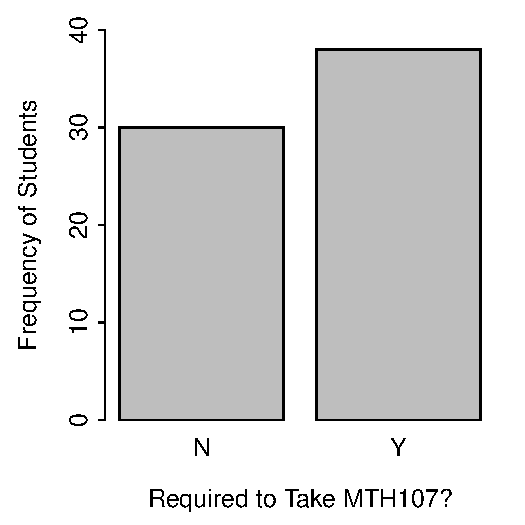
\includegraphics[width=.4\linewidth]{Figs/MTH107BarChart-1} 
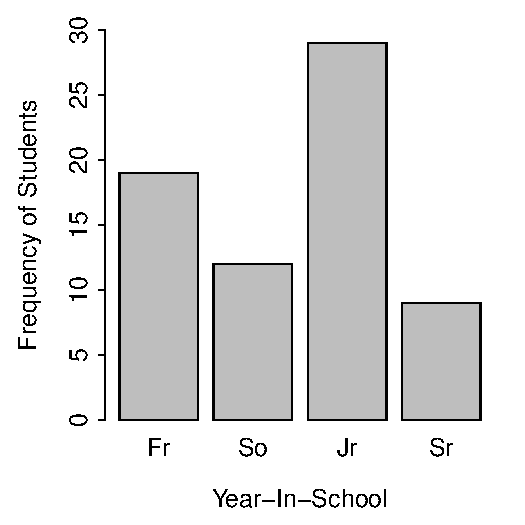
\includegraphics[width=.4\linewidth]{Figs/MTH107BarChart-2} 

}

\caption[Bar charts of the frequency of individuals in MTH107 during Winter 2010 by whether or not they were required to take MTH107 (\textbf{Left}) and year-in-school (\textbf{Right})]{Bar charts of the frequency of individuals in MTH107 during Winter 2010 by whether or not they were required to take MTH107 (\textbf{Left}) and year-in-school (\textbf{Right}).}\label{fig:MTH107BarChart}
\end{figure}


\end{knitrout}

\warn{Bar charts are used to display the frequency of individuals in the categories of a categorical variable. Histograms are used to display the frequency of individuals in classes created from quantitative variables.}

\vspace{-12pt}
\warn{Do not describe shape, center, dispersion, and outliers for a categorical variable.}

\subsection{Bar Plots in R} \label{sect:BarChart}\index{Bar Chart!Construction}
\vspace{-12pt}
A bar plot is produced by giving the saved \R{xtabs()} object as the first argument to \R{barplot()}. The x- and y-axes may be explicitly labeled with \R{xlab=} and \R{ylab=}, respectively.  For example, the bar plot for the recycling data \figrefp{fig:Barchart1} is produced below.
\begin{knitrout}
\definecolor{shadecolor}{rgb}{0.922, 0.922, 0.922}\color{fgcolor}\begin{kframe}
\begin{verbatim}
> barplot(tabRecycle,ylab="Frequency",xlab="Recycle Response")
\end{verbatim}
\end{kframe}\begin{figure}[hbtp]

{\centering 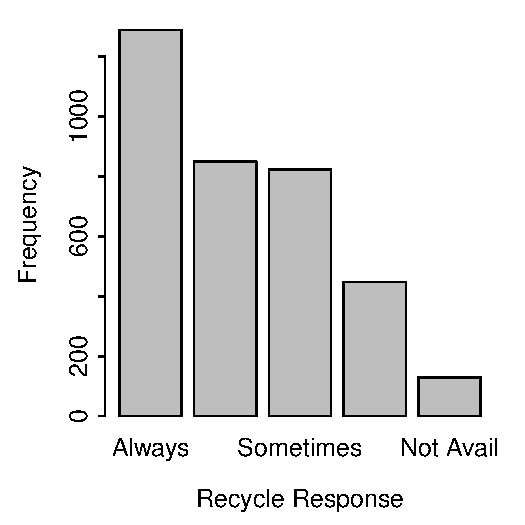
\includegraphics[width=.55\linewidth]{Figs/Barchart1-1} 

}

\caption[Bar chart of the frequency of responses to the recycling question on the GSS]{Bar chart of the frequency of responses to the recycling question on the GSS.}\label{fig:Barchart1}
\end{figure}


\end{knitrout}

\vspace{-12pt}
\begin{exsection}
  \item \label{revex:EDAArsenic2} \rhw{} Use the \href{https://raw.githubusercontent.com/droglenc/NCData/master/Arsenic.csv}{Arsenic.csv} data in Exercise \ref{revex:EDAArsenic1} to answer the questions below. \ansref{ans:EDAArsenic2}
  \begin{Enumerate}
    \item Construct a univariate EDA for the assessment of drinking water usage.
    \item Construct a univariate EDA for the assessment of cooking water usage.
  \end{Enumerate}

  \item \label{revex:cuEDAEPA}The Environmental Protection Agency (EPA) commissioned the Gallup Organization to conduct a nationwide telephone survey of 1000 households during August and September of 2002 regarding consumer knowledge and satisfaction with drinking water quality.  Of the 1000 respondents surveyed, 751 knew that their drinking water came from a public or commercial water supplier.  Of these 751 respondents, the following percentages knew precisely where that water was derived:

  \begin{center}
  \begin{tabular}{c|c|c|c|c|c}
    \hline\hline
    Ground- & Lake/ &  & Multiple & Don't & Refused \\
    water & Reservoir & River & Sources & Know & Answer \\
    \hline
    15.9\% & 29.2\% & 9.6\% & 15.7\% & 29.4\% & 0.2\% \\
    \hline\hline
  \end{tabular}
  \end{center}

  Use these data to answer the questions below. \ansref{ans:cuEDAEPA}
  \begin{Enumerate}
    \item Construct a frequency table of these data (note percentages above were rounded).
    \item Write a brief conclusion derived from these data.
  \end{Enumerate}

  \item \label{revex:cuEDAHI} \rhw{} A neighborhood in Honolulu conducted a survey to determine if residents participated in the curbside recycling program.  One question on their survey was, ``How much has curbside recycling reduced your regular refuse? 0\%, 25\%, 50\%, 75\%, 100\%, or `too early to tell'?''  The individual responses for the returned surveys are shown below with letters corresponding to the category choices offered (e.g., \verb"A"=0\%, \verb"B"=25\%, and so on).

  \begin{Verbatim}
C, C, B, B, B, B, C, E, B, B, C, B, C, B, C, C, C, E, B, B, B,
C, B, B, C, C, C, B, C, B, C, B, B, C, B, C, B, B, B, C, E, B,
E, B, B, C, C, B, B, B, E, B, C, C, C, B, B, C, B, B, B, B, B
  \end{Verbatim}

  Use these data to answer the questions below. \ansref{ans:cuEDAHI}
  \begin{Enumerate}
    \item Construct a frequency table of these data.
    \item Construct a percentage table of these data.
    \item Write a brief conclusion derived from these data.
  \end{Enumerate}

  \item \label{revex:cuEDARice} \rhw{} Students in a senior level environmental studies class at Rice University conducted a voluntary response survey regarding water usage by their peers.  They received returned surveys from a total 130 students.  One question on their survey was, ``On average, for how many minutes do you let the water run each time you take a shower? 0-5, 6-10, 11-15, or over 15 minutes?''  The individual responses for this survey are shown below with letters corresponding to the category choices offered (e.g., \verb"A"=``0-5'', \verb"B"=``6-10'', and so on). \ansref{ans:cuEDARice}

  \begin{Verbatim}
  D, C, B, B, C, C, B, B, C, C, C, B, D, B, C, C, B, C, D, D,
  B, C, C, A, B, C, C, A, C, C, D, A, C, C, B, B, B, B, B, C,
  D, B, D, B, C, B, C, C, D, C, B, B, D, C, B, C, B, B, C, C,
  B, C, B, C, B, B, C, D, B, C, D, C, B, C, D, C, C, B, C, B,
  D, B, B, D, B, C, B, B, C, B, C, D, D, C, D, B, B, C, B, C,
  A, A, B, C, B, C, D, D, C, B, D, C, C, C, C, A, C, D, B, C,
  B, B, D, C, B, B, A, B, C, B
  \end{Verbatim}

  Use these data to answer the questions below.
  \begin{Enumerate}
    \item Construct a frequency table of these data.
    \item Construct a percentage table of these data.
    \item Write a brief conclusion derived from these data.
  \end{Enumerate}
\end{exsection}


\section{Example Interpretations}\index{EDA!Univariate!Quantitative}
For categorical data, an appropriate EDA consists of identifying the major characteristics among the categories. Shape, center, dispersion, and outliers are NOT described for categorical data because the data is not numerical and, if nominal, no order exists.  In general, the major characteristics of the table or graph are described from an intuitive basis.  For example, there were more males than females in the Winter 2010 MTH107 class and mostly juniors and Freshmen. Other examples are below.

\subsection{Mixture Seed Count}
\vspace{-12pt}
\begin{quote}
\textit{A bag of seeds was purchased for seeding a recently constructed wetland.  The purchaser wanted to determine if the percentage of seeds in four broad categories -- ``grasses'', ``sedges'', ``wildflowers'', and ``legumes'' -- was similar to what the seed manufacturer advertised.  The purchaser examined a 0.25-lb sample of seeds from the bag and recorded the results in \href{https://raw.githubusercontent.com/droglenc/NCData/master/WetlandSeeds.csv}{WetlandSeeds.csv}.  Use these data to describe the distribution of seed counts into the four broad categories.}
\end{quote}



The majority of seeds were either sedge or grass with sedge being more than twice as abundant as grass (\tabref{tab:SeedTable}; \figref{fig:SeedBarplot}).  Very few legumes or wildflowers were found in the sample.

\begin{knitrout}
\definecolor{shadecolor}{rgb}{0.922, 0.922, 0.922}\color{fgcolor}\begin{figure}[hbtp]

{\centering 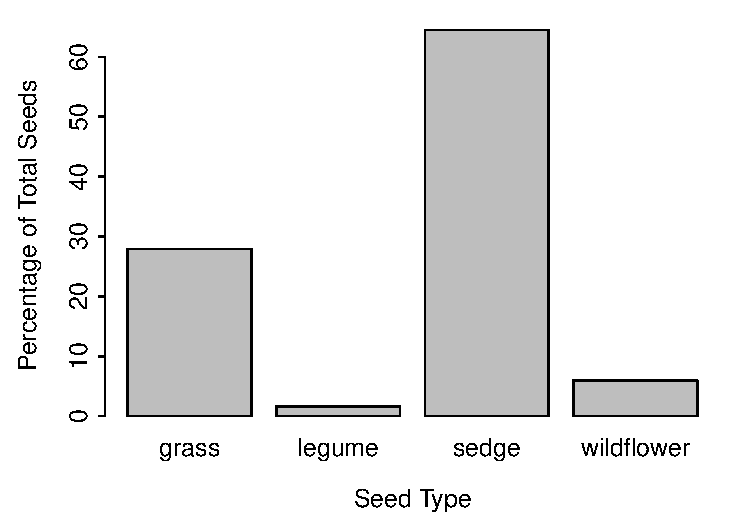
\includegraphics[width=.5\linewidth]{Figs/SeedBarplot-1} 

}

\caption[Barplot of the percentage of wetland seeds by type]{Barplot of the percentage of wetland seeds by type.}\label{fig:SeedBarplot}
\end{figure}


\end{knitrout}

% latex table generated in R 3.3.3 by xtable 1.8-2 package
% Wed Apr 26 20:49:44 2017
\begin{table}[ht]
\centering
\caption{Percentage distribution of wetland seeds by type.} 
\label{tab:SeedTable}
\begin{tabular}{rrrr}
  \hline
grass & legume & sedge & wildflower \\ 
  \hline
27.9 & 1.6 & 64.5 & 6.0 \\ 
   \hline
\end{tabular}
\end{table}


\begin{minipage}{\textwidth}
R Appendix:
\begin{knitrout}
\definecolor{shadecolor}{rgb}{0.922, 0.922, 0.922}\color{fgcolor}\begin{kframe}
\begin{verbatim}
ws <- read.csv("data/WetlandSeeds.csv")
str(ws)
wtbl <- xtabs(~type,data=ws)
percTable(wtbl,digits=1)
barplot(wptbl[-5],ylab="Percentage of Total Seeds",xlab="Seed Type")
\end{verbatim}
\end{kframe}
\end{knitrout}
\end{minipage}

\begin{exsection}
  \item \label{revex:cuEDAZoo1} \rhw{} The data in \href{https://raw.githubusercontent.com/droglenc/NCData/master/Zoo1.csv}{Zoo1.csv} contains a list of animals found in several different zoos.  In addition, each animal was classified into broad ``type'' categories (``mammal'', ``bird'', and ``amph/rep'').  Perform a univariate EDA on the \var{type} variable. \ansref{ans:cuEDAZoo1}
\end{exsection}



\chapter{Normal Distribution}  \label{chap:NormDist}
\begin{ChapObj}{\boxwidth}
  \textbf{Objectives:}
  \begin{Enumerate}
    \item Describe what a normal distribution looks like and what parameters control its shape.
    \item Describe simple properties describing the distribution of individuals on a normal distribution.
    \item Compute the proportion of individuals with a particular set of values from a normal distribution (``forward'' calculations).
    \item Compute the range of values for a certain proportion of individuals from a normal distribution (``reverse'' calculations).
  \end{Enumerate}
\end{ChapObj}

\minitoc
\newpage


\lettrine{A}{ model for the distribution} of a single quantitative variable can be visualized by ``fitting'' a smooth curve to a histogram, removing the histogram, and using the remaining curve as a model for the distribution of the entire population of individuals.  This process is illustrated with the three figures shown in \figref{fig:NormDensityEx}.  The underlying histogram was computed from the individuals in a very large sample.  The smooth red curve was drawn over the histogram and then removed to serve as a model for the distribution of the entire population.\index{Population Distribution!Normal Distribution}  If the smooth curve follows a known distribution, then certain calculations are greatly simplified.

\begin{knitrout}
\definecolor{shadecolor}{rgb}{0.922, 0.922, 0.922}\color{fgcolor}\begin{figure}[hbtp]

{\centering 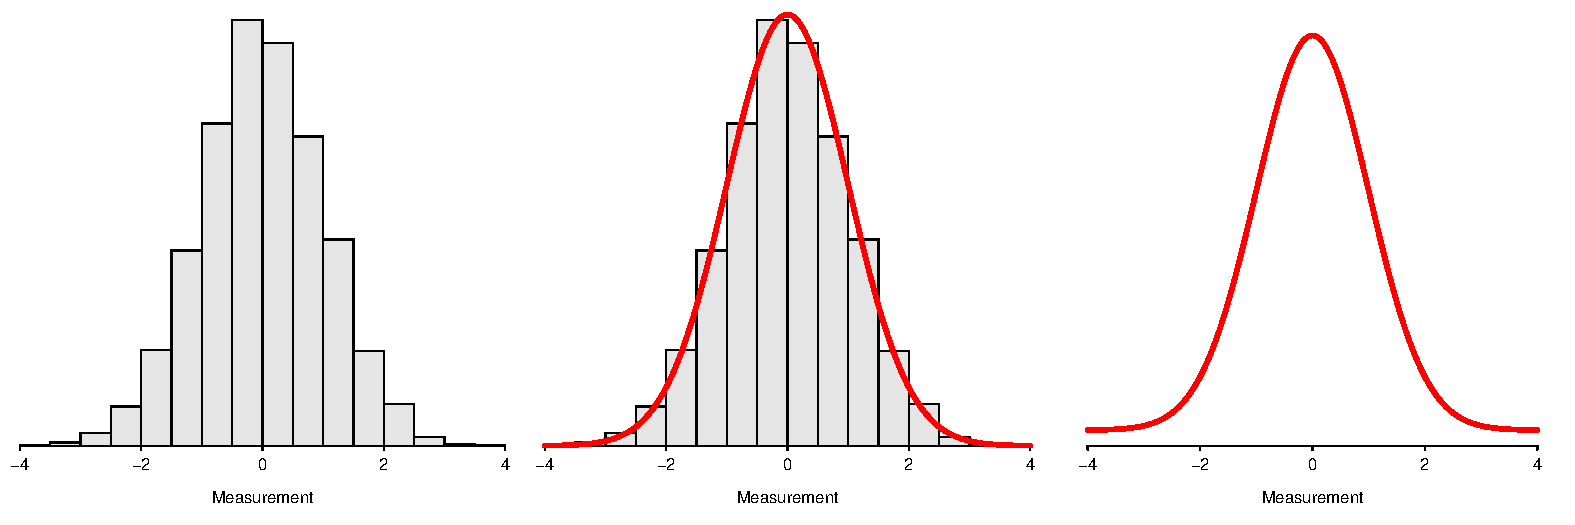
\includegraphics[width=.95\linewidth]{Figs/NormDensityEx-1} 

}

\caption[Depiction of fitting a smooth curve to a histogram and then removing the histogram to leave the smooth curve model]{Depiction of fitting a smooth curve to a histogram and then removing the histogram to leave the smooth curve model.}\label{fig:NormDensityEx}
\end{figure}


\end{knitrout}

The normal distribution is one of the most important distributions in statistics because it serves as a model for the distribution of individuals in many natural situations and the distribution of statistics from repeated samplings (i.e., sampling distributions).\footnote{See \modref{chap:SamplingDist}.}  The use of a normal distribution model to make certain calculations is demonstrated in this module.

\section{Characteristics of a Normal Distribution}\index{Normal Distribution!Characteristics}
The normal distribution is the common bell-shaped curve that you are probably familiar with (\figref{fig:NormDensityEx}-Right).  Normal distributions are abstractions of reality that are meant to represent all of the individuals in a population.  The height of the curve at a value of $x$ is found with
\begin{equation}
  \label{eqn:NormDistfx}
    f(x) = \frac{1}{\sigma\sqrt{2\pi}}e^{-\frac{1}{2}\left(\frac{x-\mu}{\sigma}\right)^{2}}
\end{equation}
which has two parameters\footnote{The $e$ and $\pi$ are the usual numerical constants.} -- the population mean, $\mu$,\index{Mean!Population symbol} and the population standard deviation, $\sigma$.\index{Standard Deviation!Population symbol}  The mean, $\mu$, controls the center and the standard deviation, $\sigma$, controls the dispersion of the distribution \figrefp{fig:NormMultDists}.

\begin{knitrout}
\definecolor{shadecolor}{rgb}{0.922, 0.922, 0.922}\color{fgcolor}\begin{figure}[hbtp]

{\centering 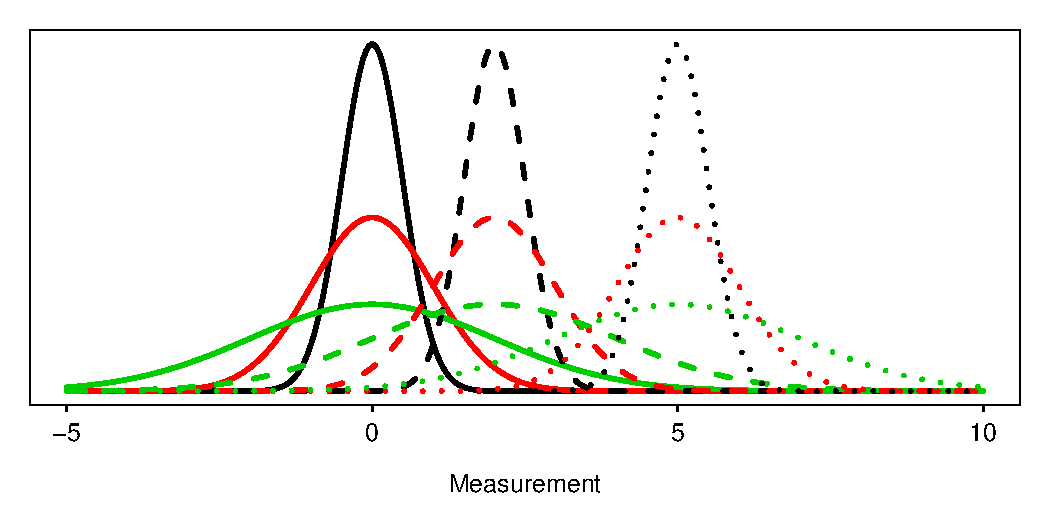
\includegraphics[width=.8\linewidth]{Figs/NormMultDists-1} 

}

\caption[Multiple normal distributions]{Multiple normal distributions.  Distributions with the same line type have the same value of $\mu$.  Distributions with the same color have the same value of $\sigma$.  Values of $\mu$ are 0 (solid), 2 (dashed), and 5 (dotted).  Values of $\sigma$ are 0.5 (black), 1 (red), and 2 (green).}\label{fig:NormMultDists}
\end{figure}


\end{knitrout}

\warn{It is not important that you remember the equation for the height of a normal distribution; however, you do need to remember that the exact position and width of the normal distribution is controlled \textsc{\textbf{only}} by the values of $\mu$ and $\sigma$.}

\begin{minipage}{\textwidth}
There are an infinite number of normal distributions because there are an infinite number of combinations of $\mu$ and $\sigma$.  However, each normal distribution will
\begin{Enumerate}
  \item be bell-shaped and symmetric,
  \item centered at $\mu$,
  \item have inflection points at $\mu \pm \sigma$, and
  \item have a total area under the curve equal to 1.
\end{Enumerate}
\end{minipage}

\warn{All normal distributions are bell-shaped. The center and dispersion of each, though, is dictated by the values of $\mu$ and $\sigma$, respectively.}

If a generic variable $X$ follows a normal distribution with a mean of $\mu$ and a standard deviation of $\sigma$, then it is said that $X\sim N(\mu,\sigma)$.\index{Normal Distribution!Symbol}  For example, if the heights of students ($H$) follows a normal distribution with a $\mu$ of 66 and a $\sigma$ of 3, then it is said that $H\sim N(66,3)$.  As another example, $Z\sim N(0,1)$ means that the variable $Z$ follows a normal distribution with a mean of $\mu$=0 and a standard deviation of $\sigma$=1.

\warn{A generic variable $X$ that is normally distributed with a mean of $\mu$ and standard deviation of $\sigma$ is abbreviated as $X\sim N(\mu,\sigma)$.}



\section{Simple Areas Under the Curve}
\vspace{-8pt}
A common statistical problem is to determine the proportion of individuals with a value of the variable between two numbers.  For example, you might be faced with determining the proportion of all sites that have lead concentrations between 1.2 and 1.5 $\mu g \cdot m^{-3}$, the proportion of students that scored higher than 700 on the SAT, or the proportion of Least Weasels that are shorter than 150 mm.  Before considering these more realistic situations, we explore calculations for the generic variable $X$ shown in \figref{fig:NormDistShade}.

Let's consider finding the proportion of individuals in a \textit{sample} with values between 0 and 2.  A histogram can be used to answer this question because it is about the individuals in a sample (\figref{fig:NormDistShade}-Left).  In this case, the proportion of individuals with values between 0 and 2 is computed by dividing the number of individuals in the red shaded bars by the total number of individuals in the histogram.  The analogous computation on the superimposed smooth curve is to find the area under the curve between 0 and 2 (\figref{fig:NormDistShade}-Right).  The area under the curve is a ``proportion of the total'' because, as stated above, the area under the entire curve is equal to 1.  The actual calculations on the normal curve will be shown in the following sections.  However, at this point, note that the calculation of an area on a normal curve is analogous to summing the number of individuals in the appropriate classes of the histogram and dividing by $n$.

\begin{knitrout}
\definecolor{shadecolor}{rgb}{0.922, 0.922, 0.922}\color{fgcolor}\begin{figure}[hbtp]

{\centering 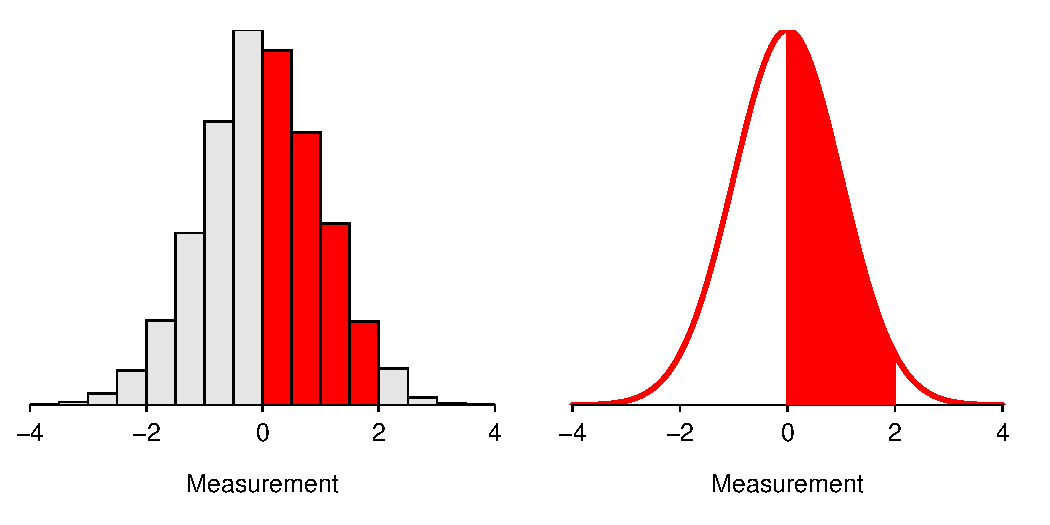
\includegraphics[width=.8\linewidth]{Figs/NormDistShade-1} 

}

\caption[Depiction of finding the proportion of individuals between 0 and 2 on a histogram (\textbf{Left}) and on a standard normal distribution (\textbf{Right})]{Depiction of finding the proportion of individuals between 0 and 2 on a histogram (\textbf{Left}) and on a standard normal distribution (\textbf{Right}).}\label{fig:NormDistShade}
\end{figure}


\end{knitrout}

\warn{The proportion of individuals between two values of a variable that is normally distributed is the area under the normal distribution between those two values.}

The 68-95-99.7 Rule\footnote{Other authors call this the ``Empirical Rule.''} states that 68\% of the individuals that follow a normal distribution will have values between $\mu-1\sigma$ and $\mu+1\sigma$, 95\% will be between $\mu-2\sigma$ and $\mu+2\sigma$, and 99.7\% will be between $\mu-3\sigma$ and $\mu+3\sigma$ \figrefp{fig:NormEmpiricalRule}.\index{Normal Distribution!68-95-99.7\% Rule}\index{68-95-99.7\% Rule}  The 68-95-99.7 Rule is true no matter what $\mu$ and $\sigma$ are as long as the distribution is normal.  For example, if $A\sim N(3,1)$, then 68\% of the individuals will fall between 2 (i.e., 3-1*1) and 4 (i.e., 3+1*1) and 99.7\% will fall between 0 (i.e., 3-3*1) and 6 (i.e., 3+3*1).  Alternatively, if $B\sim N(9,3)$, then 68\% of the individuals will fall between 6 (i.e., 9-1*3) and 12 (i.e., 9+1*3) and 95\% will be between 3 (i.e., 9-2*3) and 15 (i.e., 9+2*3).  Similar calculations can be made for any normal distribution.

\begin{knitrout}
\definecolor{shadecolor}{rgb}{0.922, 0.922, 0.922}\color{fgcolor}\begin{figure}[hbtp]

{\centering 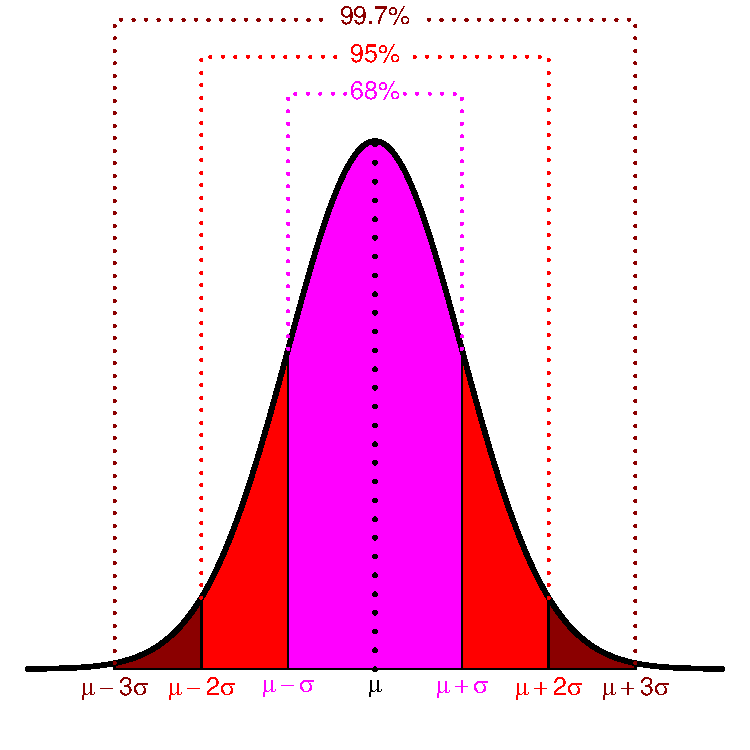
\includegraphics[width=.5\linewidth]{Figs/NormEmpiricalRule-1} 

}

\caption[Depiction of the 68-95-99.7 (or Empirical) Rule on a normal distribution]{Depiction of the 68-95-99.7 (or Empirical) Rule on a normal distribution.}\label{fig:NormEmpiricalRule}
\end{figure}


\end{knitrout}

\defn{68-95-99.7 Rule}{For all normal distributions 68\% of the individuals will be between $\mu\pm1\sigma$, 95\% will be between $\mu\pm2\sigma$, and 99.7\% will be between $\mu\pm3\sigma$}

The 68-95-99.7 Rule is used to find areas under the normal curve as long as the value of interest is an \textbf{integer} number of standard deviations away from the mean.  For example, the proportion of individuals that have a value of A greater than 5 is found by first realizing that 95\% of the individuals on this distribution fall between 1 and 5.  By subtraction this means that 5\% of the individuals must be less than 1 \textbf{AND} greater than 5.  Finally, because normal distributions are symmetric, the same proportion of individuals must be less than 1 as are greater than 5.  Thus, half of 5\%, or 2.5\%, of the individuals have a value of A greater than 5.

\warn{The 68-95-99.7 Rule can only be used for questions involving \textbf{integer} standard deviations away from the mean.}

\begin{exsection}
  \item \label{revex:quNorm68} On any normal distribution, what percentage of the individuals is within $\pm1\sigma$ of $\mu$? \ansref{ans:quNorm68}
  \item \label{revex:quNorm68gt} On any normal distribution, what percentage of the individuals are greater than $\mu+\sigma$? \ansref{ans:quNorm68gt}
  \item \label{revex:quNorm95gt} On any normal distribution, what percentage of the individuals are greater than $\mu-2\sigma$? \ansref{ans:quNorm95gt}
  \item \label{revex:quNormbt6895} On any normal distribution, what percentage of the individuals are between $\mu-2\sigma$ and $\mu+1\sigma$? \ansref{ans:quNormbt6895}
  \item \label{revex:quNorm84} On a N(-1,1) distribution, what percentage of the individuals are negative? \ansref{ans:quNorm84}
  \item \label{revex:quNorm16} On a N(100,20) distribution, what percentage of the individuals are less than 80? \ansref{ans:quNorm16}
  \item \label{revex:quNorm16a} On a N(-20,100) distribution, what percentage of the individuals are greater than 80? \ansref{ans:quNorm16a}
  \item \label{revex:quNormAB} Identify the mean and standard deviation for each population on the graph below (HINT: ``eyeball'' integers). \ansref{ans:quNormAB}

    \begin{center}
      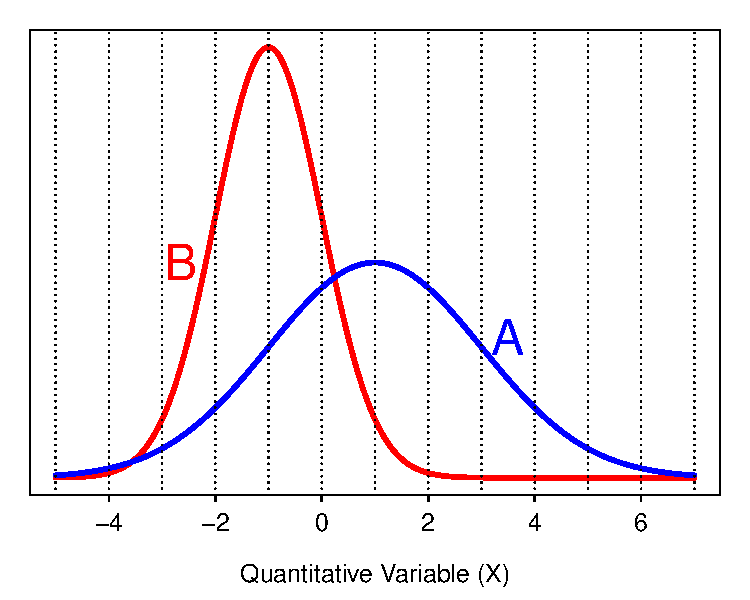
\includegraphics[width=3in]{Figs/Guess-1}
    \end{center}
\end{exsection}


\section[Forward Calculations]{More Complex Areas (Forward Calculations)}
\vspace{-12pt}
Areas under the curve relative to non-integer numbers of standard deviations away from the mean used to be found via a calculation and examination of a so-called standard normal table.  With the advent of computers and cheap software these areas are now found simply with the aid of computer software like R.

The area under a normal curve relative to a particular value is computed in R with \R{distrib()}.  This function requires the \textit{particular value} as the first argument and the mean and standard deviation of the normal distribution in the \R{mean=} and \R{sd=} arguments, respectively.  The \R{distrib()} function defaults to finding the area under the curve to the \textbf{left of} the particular value, but it can find the area under the curve to the right of the particular value by including \R{lower.tail=FALSE}.

For example, suppose that the heights of a population of students, represented by $H$, is known to be $H\sim N(66,3)$.  Thus, the proportion of students in this population that have a height less than 71 inches is computed below. Thus, approximately 95.2\% of the students in this population have a height less than 71 inches \figrefp{fig:NormZCalc1}.
\begin{knitrout}
\definecolor{shadecolor}{rgb}{0.922, 0.922, 0.922}\color{fgcolor}\begin{kframe}
\begin{verbatim}
> ( distrib(71,mean=66,sd=3) )
[1] 0.9522096
\end{verbatim}
\end{kframe}\begin{figure}[hbtp]

{\centering \includegraphics[width=.4\linewidth]{Figs/NormZCalc1-1} 

}

\caption[Calculation of the proportion of individuals on a $N(66,3)$ with a value less than 71]{Calculation of the proportion of individuals on a $N(66,3)$ with a value less than 71.}\label{fig:NormZCalc1}
\end{figure}


\end{knitrout}

The proportion of students in this population that have a height \textit{greater} than 68 inches is computed below (note use of \R{lower.tail=FALSE}). Thus, approximately 25.2\% of the students in this population have a height greater than 68 inches \figrefp{fig:NormZCalc2}.
\begin{knitrout}
\definecolor{shadecolor}{rgb}{0.922, 0.922, 0.922}\color{fgcolor}\begin{kframe}
\begin{verbatim}
> ( distrib(68,mean=66,sd=3,lower.tail=FALSE) )
[1] 0.2524925
\end{verbatim}
\end{kframe}\begin{figure}[hbtp]

{\centering \includegraphics[width=.4\linewidth]{Figs/NormZCalc2-1} 

}

\caption[Calculation of the proportion of individuals on a $N(66,3)$ with a value greater than 68]{Calculation of the proportion of individuals on a $N(66,3)$ with a value greater than 68.}\label{fig:NormZCalc2}
\end{figure}


\end{knitrout}

\warn{The area greater than a particular value is found by including the \R{lower.tail=FALSE} argument in \R{distrib()}.}

Finding the area between two particular values is a bit more work.  To answer ``between''-type questions, the area less than the smaller of the two values is subtracted from the area less than the larger of the two values.  This is illustrated by noting that two values split the area under the normal curve into three parts -- A, B, and C \figrefp{fig:NormDistBetween}.  The area between the two values is B.  The area to the left of the larger value corresponds to the area A+B.  The area to the left of the smaller value corresponds to the area A.  Thus, subtracting the latter from the former leaves the ``in-between'' area B (i.e., (A+B)-A = B).

\begin{knitrout}
\definecolor{shadecolor}{rgb}{0.922, 0.922, 0.922}\color{fgcolor}\begin{figure}[hbtp]

{\centering \includegraphics[width=.4\linewidth]{Figs/NormDistBetween-1} 

}

\caption[Schematic representation of how to find the area between two $Z$ values]{Schematic representation of how to find the area between two $Z$ values.}\label{fig:NormDistBetween}
\end{figure}


\end{knitrout}
\vspace{12pt} % because the spacing is gobbled by the R code.

For example, the area between 62 and 70 inches of height is found below (intermediate calculations shown in \figref{fig:NormZCalc3}). Thus, 81.8\% of students in this population have a height between 62 and 70 inches.

\begin{knitrout}
\definecolor{shadecolor}{rgb}{0.922, 0.922, 0.922}\color{fgcolor}\begin{kframe}
\begin{verbatim}
> ( AB <- distrib(70,mean=66,sd=3) )
[1] 0.9087888
> ( A <- distrib(62,mean=66,sd=3) )
[1] 0.09121122
> AB-A
[1] 0.8175776
\end{verbatim}
\end{kframe}\begin{figure}[hbtp]

{\centering \includegraphics[width=.4\linewidth]{Figs/NormZCalc3-1} 
\includegraphics[width=.4\linewidth]{Figs/NormZCalc3-2} 

}

\caption[Calculation of the areas less than 70 inches (\textbf{Left}) and 62 inches (\textbf{Right})]{Calculation of the areas less than 70 inches (\textbf{Left}) and 62 inches (\textbf{Right}).}\label{fig:NormZCalc3}
\end{figure}


\end{knitrout}

\warn{The area between two values is found by subtracting the area less than the smaller value from the area less than the larger value.}

\begin{exsection}
  \item \label{revex:quNormZ0.11} If $X\sim N(0,1)$, then what is the percentage of $X<0.11$? \ansref{ans:quNormZ0.11}
  \item \label{revex:quNormZm0.11} If $X\sim N(0,1)$, then what is the percentage of $X>-0.11$? \ansref{ans:quNormZm0.11}
  \item \label{revex:quNormZbtwn} If $X\sim N(0,1)$, then what is the percentage of $-1.45<X<1.11$? \ansref{ans:quNormZbtwn}
  \item \label{revex:quNormXgt75} If $Y\sim N(70,6)$, then what is the percentage of $Y>75$? \ansref{ans:quNormXgt75}
  \item \label{revex:quNormXlt63} If $Y\sim N(70,6)$, then what is the percentage of $Y<63$? \ansref{ans:quNormXlt63}
  \item \label{revex:quNormXbtwn} If $Y\sim N(70,6)$, then what is the percentage of $62.3<Y<72.9$? \ansref{ans:quNormXbtwn}
\end{exsection}


\section[Reverse Calculations]{Values from Areas (Reverse Calculations)}
Another important calculation with normal distributions is finding the value or values of $X$ with a given proportion of individuals less than, greater than, or between.  For example, it may be necessary to find the test score such that 90\% (or 0.90 as a proportion) of the students scored lower.  In contrast to the calculations in the previous section (where the value of $X$ was given and a proportion of individuals was asked for), the calculations in this section give a proportion and ask for a value of $X$.  These types of questions are called \textbf{``reverse'' normal distribution questions} to contrast them with questions from the previous section.

Reverse questions are also answered with \R{distrib()}, though the first argument is the proportion (or area) of interest.  The calculated will be treated as a ``reverse'' question when \R{type="q"} is given to \R{distrib()}.\footnote{``q'' stands for quantile.}  For example, the height that has 20\% of all students shorter is  63.5 inches, as computed below \figrefp{fig:NormZCalc4}.
\begin{knitrout}
\definecolor{shadecolor}{rgb}{0.922, 0.922, 0.922}\color{fgcolor}\begin{kframe}
\begin{verbatim}
> ( distrib(0.20,mean=66,sd=3,type="q") )
[1] 63.47514
\end{verbatim}
\end{kframe}\begin{figure}[hbtp]

{\centering \includegraphics[width=.4\linewidth]{Figs/NormZCalc4-1} 

}

\caption[Calculation of the height with 20\% of all students shorter]{Calculation of the height with 20\% of all students shorter.}\label{fig:NormZCalc4}
\end{figure}


\end{knitrout}

``Greater than'' reverse questions are computed by including \R{lower.tail=FALSE}.  For example, 10\% of the population of students is taller than 69.8 inches, as computed below \figrefp{fig:NormZCalc5}.
\begin{knitrout}
\definecolor{shadecolor}{rgb}{0.922, 0.922, 0.922}\color{fgcolor}\begin{kframe}
\begin{verbatim}
> ( distrib(0.10,mean=66,sd=3,type="q",lower.tail=FALSE) )
[1] 69.84465
\end{verbatim}
\end{kframe}\begin{figure}[hbtp]

{\centering \includegraphics[width=.4\linewidth]{Figs/NormZCalc5-1} 

}

\caption[Calculation of the height with 10\% of all students taller]{Calculation of the height with 10\% of all students taller.}\label{fig:NormZCalc5}
\end{figure}


\end{knitrout}

``Between'' questions can only be easily handled if the question is looking for endpoint values that are symmetric about $\mu$.  In other words, the question must ask for the two values that contain the ``most common'' proportion of individuals.  For example, suppose that you were asked to find the most common 80\% of heights.  This type of question is handled by converting this ``symmetric between'' question into two ``less than'' questions.  For example, in \figref{fig:NormRevBetween} the area D is the symmetric area of interest.  If D is 0.80, then C+E must be 0.20.\footnote{Because all three areas must sum to 1.}  Because D is symmetric about $mu$, C and E must both equal 0.10.  Thus, the lower bound on D is the value that has 10\% of all values smaller.  Similarly, because the combined area of C and D is 0.90, the upper bound on D is the value that has 90\% of all values smaller.  This question has now been converted from a ``symmetric between'' to two ``less than'' questions that can be answered exactly as shown above.  For example, the two heights that have a symmetric 80\% of individuals between them are 62.2 and 69.8 as computed below.
\begin{knitrout}
\definecolor{shadecolor}{rgb}{0.922, 0.922, 0.922}\color{fgcolor}\begin{kframe}
\begin{verbatim}
> ( distrib(0.10,mean=66,sd=3,type="q") )
[1] 62.15535
> ( distrib(0.90,mean=66,sd=3,type="q") )
[1] 69.84465
\end{verbatim}
\end{kframe}
\end{knitrout}

\begin{knitrout}
\definecolor{shadecolor}{rgb}{0.922, 0.922, 0.922}\color{fgcolor}\begin{figure}[hbtp]

{\centering \includegraphics[width=.4\linewidth]{Figs/NormRevBetween-1} 

}

\caption[Depiction of areas in a reverse between type normal distribution question]{Depiction of areas in a reverse between type normal distribution question.}\label{fig:NormRevBetween}
\end{figure}


\end{knitrout}

\begin{exsection}
  \item \label{revex:quNormXrev03} If $Y\sim N(70,6)$, then what is Y such that the area to the left of it is 0.3? \ansref{ans:quNormXrev03}
  \item \label{revex:quNormXrev04} If $Y\sim N(70,6)$, then what is Y such that the area to the right of it is 0.4? \ansref{ans:quNormXrev04}
  \item \label{revex:quNormXrev05} If $Y\sim N(70,6)$, then what are the Ys such that the area between them is 0.5? \ansref{ans:quNormXrev05}
\end{exsection}


\subsection{Distinguish Calculation Types}\index{Normal Distribution!Finding areas}\index{Normal Distribution!Finding values}
It is critical to be able to distinguish between the two main types of calculations made from normal distributions.  The first type of calculation is a ``forward'' calculation where the area or proportion of individuals relative to a value of the variable must be found.  The second type of calculation is a ``reverse'' calculation where the value of the variable relative to a particular area is calculated.

Distinguishing between these two types of calculations is a matter of deciding if (i) the value of the variable is given and the proportion (or area) is to be found or (ii) if the proportion (or area) is given and the value of the variable is to be found.  Therefore, distinguishing between the calculation types is as simple as identifying what is given (or known) and what must be found.  If the value of the variable is given but not the proportion or area, then a forward calculation is used.  If the area or proportion is given, then a reverse calculation to find the value of the variable is used.

\newpage
\begin{exsection}
  \item \label{revex:quNormStudentAge} The age at which ``traditional'' students graduate from college is N(22.1, 1.1).  Use this information to answer the questions below. \ansref{ans:quNormStudentAge}
\begin{Enumerate}
  \item What percentage of the students graduate by the age of 21?
  \item What percentage of the students graduate after age 24?
  \item What is the age range for the middle 95\% of the students?
  \item What is the age at which 90\% of the students have graduated?
\end{Enumerate}

  \item \label{revex:quNormBlackBears} We know, from years of study of black bears, that the population distributions for head length is N(13.7,1.9), neck girth is N(20.9,4.8), and body length is N(60.0,10). All other variables measured on black bears cannot be described by a normal distribution.  Use this information to answer the questions below. \ansref{ans:quNormBlackBears}
\begin{Enumerate}
  \item What is the percentage of bears between 45" and 65" in body length?
  \item What is the percentage of bears that weighs more than 200 lbs?
\end{Enumerate}

  \item \label{revex:quNormShrews} The brain weights of short-tailed shrews (\textit{Blarina brevicauda}) is normally distributed with a mean of 0.14 grams and a standard deviation of 0.04 grams. Use this information to answer the questions below. \ansref{ans:quNormShrews}
\begin{Enumerate}
  \item What percentage of shrews have a brain weight less than 0.09 grams?
  \item What percentage of shrews have a brain weight between 0.09 and 0.17 grams?
  \item What is the brain weight such that 30\% of all shrews have a larger brain weight?
\end{Enumerate}

  \item \label{revex:quNormBart} The distribution of arrival times for the BART bus at Northland is normally distributed with a mean of 0 and standard deviation of 3, where negative values indicate early arrivals (i.e., before the scheduled time) and positive values indicate late arrivals.  Use this information to answer the questions below.  \ansref{ans:quNormBart}
\begin{Enumerate}
  \item What percentage of the arrivals are more than 5 minutes late?
  \item What percentage of the arrivals are more than 4 minutes early?
  \item What percentage of the arrivals are between 4 minutes early and 4 minutes late?
  \item What is the arrival time such that 25\% of all arrival times are later than that time?
  \item What are the most common 60\% of arrival times?
  \item What kind of variable is arrival time?
\end{Enumerate}

  \item \label{revex:quNormRoeDeer} Researchers on Storfosna Is., Norway wanted to examine reproductive habits of roe deer \textit{Capreolus capreolus} in the northern extremities \citep{AndersenLinnell2000}.  The researchers observed how many fawns were born to each of 149 female, sexually mature roe deer between the years 1991 and 1994.  The mean number of fawns from each deer was 2.235 with a standard deviation of 0.460.  Use this information to answer the questions below. \ansref{ans:quNormRoeDeer}
\begin{Enumerate}
  \item What percentage of does have less than 2 fawns.
  \item What percentage of does have more than 3 fawns.
  \item What percentage of does have between 1 and 3 fawns.
  \item What is the number of fawns such that only 7.6\% of the does have fewer fawns?
  \item What is the number of fawns such that only 4.2\% of the does have more fawns?
  \item What is the most common 87\% of number of fawns born per doe?
\end{Enumerate}

  \item \label{revex:quNormCrayfish} I recently investigated the efficacy of becoming a commercial crayfisherman (crayfish = crawfish = crawdad) on the lake I live on. With carefully constructed samples I concluded that the size of crayfish was N(93,8). The market for crayfish resides in Sweden. Swedes prefer (hence, will only buy) crayfish that are between $90$ and $110$ mm long ($<90$ are too small to deal with and $>110$ taste bad).  Use this information to answer the questions below.  \ansref{ans:quNormCrayfish}
\begin{Enumerate}
  \item How many acceptably-sized crayfish could I send to market, if I could catch approximately 50,000 crayfish? [HINT: compute the proportion of preferably-sized crayfish first.]
  \item If I could find an alternative market for the larger ($>110$) crayfish, how many could I send to it (again assume that I could catch 50,000 crayfish)?
\end{Enumerate}
\end{exsection}


\vspace{-12pt}
\section{Standardization and Z-Scores}\label{sect:Standardizing}
\vspace{-12pt}
An individual that is 59 inches tall is 7 inches shorter than average if heights are $N(66,3)$. Is this a large or a small difference?  Alternatively, this same individual is $\frac{-7}{3}$ = $-2.33$ standard deviations below the mean. Thus, a height of 59 inches is relatively rare in this population because few individuals are more than two standard deviations away from the mean.\footnote{From the 68-95-99.7\% Rule.} As seen here, the relative magnitude that an individual differs from the mean is better expressed as the number of standard deviations that the individual is away from the mean.

Values are ``standardized'' by changing the original scale (inches in this example) to one that counts the number of standard deviations (i.e., $\sigma$) that the value is away from the mean (i.e., $\mu$).  For example, with the height variable (i.e., $N(66,3)$), 69 inches is one standard deviation above the mean, which corresponds to +1 on the standardized scale. Similarly, 60 inches is two standard deviations below the mean, which corresponds to -2 on the standardized scale. Finally, 67.5 inches on the original scale is one half standard deviation above the mean or +0.5 on the standardized scale.

The process of computing the number of standard deviations that an individual is away from the mean is called \textbf{standardizing}.  Standardizing is accomplished with
\begin{equation}
  \label{eqn:Zgeneral}
    Z = \frac{\text{``value''}-\text{``center''}}{\text{``dispersion''}}
\end{equation}
or, more specifically,
\begin{equation}
  \label{eqn:Zspecific}
    Z = \frac{x-\mu}{\sigma}
\end{equation}
For example, the standardized value of an individual with a height of 59 inches is $z=\frac{59-66}{3}=-2.33$. Thus, this individual's height is 2.33 standard deviations below the average height in the population.

Standardized values ($Z$) follow a $N(0,1)$.  Thus, the $N(0,1)$ is called the ``standard normal distribution.''  The relationship between $X$ and $Z$ is one-to-one meaning that each value of $X$ converts to one and only one value of $Z$.  This means that the area to the left of $X$ on a $N(\mu,\sigma)$ is the same as the area to the left of $Z$ on a $N(0,1)$.  This one-to-one relationship is illustrated in \figref{fig:NormStandardizingEx} using the individual with a height of 59 inches and $Z=-2.33$.

\vspace{-6pt}
\warn{The standardized scale (i.e., z-scores) represents the number of standard deviations that a value is from the mean.}

\begin{knitrout}
\definecolor{shadecolor}{rgb}{0.922, 0.922, 0.922}\color{fgcolor}\begin{figure}[hbtp]

{\centering \includegraphics[width=.4\linewidth]{Figs/NormStandardizingEx-1} 
\includegraphics[width=.4\linewidth]{Figs/NormStandardizingEx-2} 

}

\caption{Plots depicting the area to the left of 59 on a $N(66,3)$ (\textbf{Left}) and the area to the right of the corresponding Z-score of $Z=-2.33$ on a $N(0,1)$ (\textbf{Right}).  Not that the x-axis scales are different.}\label{fig:NormStandardizingEx}
\end{figure}


\end{knitrout}



\chapter{Bivariate EDA - Quantitative} \label{chap:BivEDAQuant}
\begin{ChapObj}{\boxwidth}
  \textbf{Objectives:}
  \begin{Enumerate}
    \item Describe bivariate data.
    \item Distinguish between response and explanatory variables.
    \item Construct scatterplots of bivariate quantitative data.
    \item Describe bivariate relationships with interpretations from scatterplots.
    \item Describe how the correlation coefficient is calculated.
    \item Use the correlation coefficient to describe the strength (and association) of the relationship between two quantitative variables.
  \end{Enumerate}
\end{ChapObj}

\minitoc
\vspace{24pt}

\lettrine{B}{ivariate data occurs when two} variables have been measured on the same individuals.\index{EDA!Bivariate!Quantitative}  For example, you may measure (i) the height and weight of students in class, (ii) depth and area of a lake, (iii) gender and age of welfare recipients, or (iv) number of mice and biomass of legumes in fields. This module is focused on describing the bivariate relationship between two quantitative variables. Bivariate relationships between two categorical variables is described in \modref{chap:BivEDACat}.

\defn{Bivariate}{Data where two variables have been measured on the same individuals.}

Data on the \var{weight} (lbs) and highway miles per gallon (stored as \var{HMPG}) for 93 cars from the 1993 model year will be used as an example throughout this section.\footnote{Data are from \cite{Lock1993}.}  Ultimately, the relationship between highway MPG and the weight of a car will be examined.  These are bivariate data because measurements of both variables are recorded for each individual (i.e., a car). The following commands read the data from \href{https://raw.githubusercontent.com/droglenc/NCData/master/93cars.csv}{93cars.csv} into R and lists the \var{HMPG} and \var{weight} values for the first and last three cars\footnote{The vector in the second argument to \R{headtail()} is used to show only the two variables of interest.}.
\begin{knitrout}
\definecolor{shadecolor}{rgb}{0.922, 0.922, 0.922}\color{fgcolor}\begin{kframe}
\begin{verbatim}
> cars93 <- read.csv("data/93cars.csv")
> headtail(cars93,which=c("HMPG","Weight"))
   HMPG Weight
1    31   2705
2    25   3560
3    26   3375
91   25   2810
92   28   2985
93   28   3245
\end{verbatim}
\end{kframe}
\end{knitrout}

\section{Response and Explanatory Variables} \label{sect:RespExplan1}
\vspace{-12pt}
The \textbf{response variable} is the variable that one is interested in explaining something about (i.e., variability) or in making future predictions about.\index{Response Variable!Bivariate EDA}  Synonyms for response are dependent and predicted.  The \textbf{explanatory variable} is the variable that may help explain or allow one to predict the response variable.\index{Explanatory Variable!Bivariate EDA}  Synonyms for explanatory are independent and predictor.

\defn{Response Variable}{The variable that we are interested in explaining or predicting.  Synonyms are ``dependent'' or ``predicted'' variable.}

\vspace{-12pt}
\defn{Explanatory Variable}{The variable that we think may explain or allow us to predict the response variable. Synonyms are ``independent'' or ``predictor'' variable.}

Deciding which variable is the response variable often depends on the context of the situation (as defined by the research question).  In the first example of bivariate data given in the introduction, the response variable may be weight if interest is in predicting weight from height or it may be height if interest is in predicting height from weight.\footnote{The latter is usually not the case, though.}  The response and explanatory variables for the three situations in the introduction with quantitative variables are as follows (followed by context notes):
\begin{Itemize}
  \item R = weight, E = height [want to predict weight (hard to measure) from height (easy to measure)].
  \item R = area, E = depth [area is hard to measure, depth is easy].
  \item R = number of mice in a field, E = biomass of legumes in the field [hypothesized that higher biomass leads to more mice].
\end{Itemize}

In the car data, the weight of the car may help explain the highway MPG of the car (e.g., a hypothesis might be that heavier cars get worse gas mileage).  Thus, highway MPG is the response variable because it is of primary interest and may depend on the weight of the car.  Weight is the explanatory variable as it will be used to explain the highway MPG.

\warn{Which variable is the response variable depends on the context of the problem or the researcher's needs (i.e., which variable is being explained or predicted).}

\vspace{-6pt}
\section{Scatterplots} \index{Scatterplot!Construction}
\vspace{-12pt}
A scatterplot is a graph where each point simultaneously represents the values of both the quantiative response and quantitative explanatory variable.  The value of the explanatory variable gives the x-coordinate and the value of the response variable gives the y-coordinate of the point plotted for an individual.  For example, the first individual in the cars data is plotted at x (\var{Weight}) = 2705 and y (\var{HMPG}) = 31, whereas the second individual is at x = 3560 and y = 25.  The scatterplot for all individuals in the data file is shown in \figref{fig:carscat1}.
\begin{knitrout}
\definecolor{shadecolor}{rgb}{0.922, 0.922, 0.922}\color{fgcolor}\begin{figure}[hbtp]

{\centering \includegraphics[width=.4\linewidth]{Figs/carscat1-1} 

}

\caption[Scatterplot between the highway MPG and weight of cars manufactured in 1993]{Scatterplot between the highway MPG and weight of cars manufactured in 1993.}\label{fig:carscat1}
\end{figure}


\end{knitrout}

\warn{Both variables must be quantitative to construct a scatterplot.}

\vspace{-12pt}
\warn{Response variables are plotted on the y-axis and explanatory variables are plotted on the x-axis.}

\vspace{-6pt}
\subsection{Scatterplots in R}
\vspace{-12pt}
Scatterplots are constructed in R with \R{plot()}.  This function requires a formula of the form \R{Y\TILDE X}, where \R{Y} and \R{X} are variables to be plotted on the y- and x-axes, as the first argument, and the corresponding dataframe name in \R{data=}.\footnote{This function can also take the vector of x-axis data as its first argument followed by a vector of y-axis data as its second argument.  The formula notation is preferred for ease of transferability to other functions.} The x- and y-axis labels may be modified with \R{xlab=} and \R{ylab=}.  The scatterplot of highway MPG versus car weight \figrefp{fig:Scatplot1} was created with the code below.
\begin{knitrout}
\definecolor{shadecolor}{rgb}{0.922, 0.922, 0.922}\color{fgcolor}\begin{kframe}
\begin{verbatim}
> plot(HMPG~Weight,data=cars93,ylab="Highway MPG",xlab="Weight (lbs)")
\end{verbatim}
\end{kframe}\begin{figure}[hbtp]

{\centering \includegraphics[width=.4\linewidth]{Figs/Scatplot1-1} 

}

\caption[Scatterplot between the highway MPG and weight of cars manufactured in 1993 (using R default values)]{Scatterplot between the highway MPG and weight of cars manufactured in 1993 (using R default values)}\label{fig:Scatplot1}
\end{figure}


\end{knitrout}

The character plotted at each point can be changed with the \R{pch=} argument.\footnote{This argument is short for ``plotting character''.}  This argument defaults to a value of 1, which is an open-circle.  Numerical values used to represent other plotting characters are shown in \figref{fig:Rpch}.  For example, the scatterplot shown in \figrefp{fig:carscat1} was created by including \R{pch=16} in \R{plot()}.

\begin{knitrout}
\definecolor{shadecolor}{rgb}{0.922, 0.922, 0.922}\color{fgcolor}\begin{figure}[hbtp]

{\centering \includegraphics[width=.4\linewidth]{Figs/Rpch-1} 

}

\caption[Plotting characters available in R and their numerical codes]{Plotting characters available in R and their numerical codes. Note that for values of 21-25 that \R{bg='gray70'} is used to provide the background color.}\label{fig:Rpch}
\end{figure}


\end{knitrout}


\newpage
\section{Items to Describe}
\vspace{-12pt}
Four characteristics should be described when exploring bivariate data with a scatterplot,\index{Scatterplot!Interpretation}
\begin{Enumerate}
  \item \textbf{Association} or \textbf{Direction} of the relationship.
  \item \textbf{Form} of the relationship.
  \item \textbf{Strength} of the relationship.
  \item Presence or absence of \textbf{outliers}.
\end{Enumerate}
All four of these items can be described from the scatterplot.  It should be noted, though, that the strength of the relationship is best described with the correlation coefficient (see \sectref{sect:corr}).

Three general statements of association are used -- positive, negative, and none.\index{Association!Definitions}\index{Direction!Definitions}  A positive association is when the scatterplot resembles an increasing function (i.e., increases from lower-left to upper-right; \figref{fig:corrassn}-Right).  For a positive association, most of the individuals are above average or below average for both of the variables.  A negative association is when the scatterplot looks like a decreasing function (i.e., decreases from upper-left to lower-right; \figref{fig:corrassn}-Left).  For a negative association, most of the individuals are above average for one variable and below average for the other variable.  No association is when the scatterplot looks like a flat horizontal line or a ``shotgun blast'' of points (\figref{fig:corrassn}-Middle).  For no association, there are no tendencies for individuals to be above or below average for one variable and above or below average for the other.

\begin{knitrout}
\definecolor{shadecolor}{rgb}{0.922, 0.922, 0.922}\color{fgcolor}\begin{figure}[hbtp]

{\centering \includegraphics[width=.3\linewidth]{Figs/corrassn-1} 
\includegraphics[width=.3\linewidth]{Figs/corrassn-2} 
\includegraphics[width=.3\linewidth]{Figs/corrassn-3} 

}

\caption[Depiction of three types of association present in scatterplots]{Depiction of three types of association present in scatterplots.}\label{fig:corrassn}
\end{figure}


\end{knitrout}

\defn{Positive Association}{Most of the individuals are either above average or below average for both variables.}

\vspace{-12pt}
\defn{Negative Association}{Most of the individuals are above average for one variable and below average for the other variable.}

\vspace{-12pt}
\defn{No Association}{There are no tendencies for individuals to be above or below average for one variable and above or below average for the other variable.}

For the purposes of this introductory course, form will be defined as either linear or nonlinear.\index{Form!Definition} By default, scatterplots will be considered linear unless there is an OBVIOUS curvature in the points.  For example, all three scatterplots in \figref{fig:corrassn} are considered linear.

Strength is a summary of how closely the points cluster about the general form of the relationship.\index{Strength!Definition}  For example, for linear forms strength is how closely the points cluster around the line.  Strength is difficult to define from a scatterplot because it is a relative term.  The general idea of strength is depicted in \figref{fig:corrstrength1}.  However, an objective numerical measure -- the correlation coefficient -- is defined in \sectref{sect:corr}.

\begin{knitrout}
\definecolor{shadecolor}{rgb}{0.922, 0.922, 0.922}\color{fgcolor}\begin{figure}[hbtp]

{\centering \includegraphics[width=.8\linewidth]{Figs/corrstrength1-1} 

}

\caption[Scatterplots depicting four relatives types of strength]{Scatterplots depicting four relatives types of strength.}\label{fig:corrstrength1}
\end{figure}


\end{knitrout}

\defn{Strength}{How closely the points cluster about the general form of the relationship.}

\vspace{-12pt}
\warn{Strength can only be subjectively described from a scatterplot; use the correlation coefficient to be more objective.}

Outliers are points that are far removed from the main cluster of points.\index{Outlier}  Keep in mind (as always) that just because a point is an outlier doesn't mean it is wrong.

The relationship between highway MPG and the weight of cars \figrefp{fig:carscat1} appears to be negative, primarily linear (although I see a very slight concavity), and moderately strong.  The three points at (2400,46), (2500,27), and (1800,33) might be considered SLIGHT outliers (these are not far enough removed for me to consider them outliers, but some people may).

A general conclusion that could be made from these results is that as the weight of the cars increases, the highway MPG attained by the car decreases in a linear fashion.  While this conclusion is correct, it is also very carefully worded.  We must be very careful to not state that increasing the weight of the car CAUSES a decrease in MPG.  We cannot attribute cause because these data come from an observational study and because several other important variables were not considered in the analysis.  For example, the scatterplot in \figref{fig:carscat2}, coded for different numbers of cylinders in the car's engine, indicates that the number of cylinders may be inversely related to the highway MPG and positively related to the weight of the car.  So, does the weight of the car, the number of cylinders, or both, explain the decrease in highway MPG?

\begin{knitrout}
\definecolor{shadecolor}{rgb}{0.922, 0.922, 0.922}\color{fgcolor}\begin{figure}[hbtp]

{\centering \includegraphics[width=.4\linewidth]{Figs/carscat2-1} 

}

\caption[Scatterplot between the highway MPG and weight of cars manufactured in 1993 separated by number of cylinders]{Scatterplot between the highway MPG and weight of cars manufactured in 1993 separated by number of cylinders.}\label{fig:carscat2}
\end{figure}


\end{knitrout}

%\newpage
\begin{exsection}
  \item \label{revex:qbEDAScat} \rhw{}Researchers in Northern Wisconsin wanted to explain the role of the whitetail deer as a keystone herbivore \citep{WallerAlverson1997}.  As a part of their analysis, they examined the relationship between the mean number of hemlock saplings on 14 x 21 m sections of a woodlot and a browsing index (a complicated measurement that gives the amount of food a deer has been eating in a given area).  Use the data in the table below to make a scatterplot of the mean number of hemlock saplings versus the browsing index and describe the bivariate relationship from it. \ansref{ans:qbEDAScat}
  \begin{Verbatim}
mean no. hemlock saplings  0.95 2.89 2.97 3.94 4.74 5.10 6.64 7.13
browse index               0.31 0.35 0.49 0.50 0.61 0.63 0.86 0.90
  \end{Verbatim}
\end{exsection}


\vspace{-18pt}
\section{Correlation}\label{sect:corr}\index{Correlation!Computation}\index{Strength!Measure}
The sample correlation coefficient, abbreviated as $r$, is calculated with
\begin{equation}
  r = \frac{\Sum_{i=1}^{n}\left[\left(\frac{x_{i}-\bar{x}}{s_{x}}\right)\left(\frac{y_{i}-\bar{y}}{s_{y}}\right)\right]}{n-1}
\end{equation}
where $s_{x}$ and $s_{y}$ are the sample standard deviations for the explanatory and response variable, respectively.\footnote{See \sectref{sect:StdDev} for a review of standard deviations.}  The formulas in the two sets of parentheses in the numerator are standardized values; thus, the value in each parenthesis is called the standardized x or standardized y, respectively.\footnote{See \sectref{sect:Standardizing} for a review of standardized values.}  Using this terminology, the formula for the correlation coefficient reduces to these steps:
\begin{Enumerate}
  \item For each individual, standardize x and standardize y.
  \item For each individual, find the product of the standardized x and standardized y.
  \item Sum all of the products from step 2.
  \item Divide the sum from step 3 by n-1.
\end{Enumerate}

\warn{The sample correlation coefficient is abbreviated with $r$.  The population correlation coefficient is abbreviated with $\rho$.}

The table below illustrates these calculations for the first five individuals in the cars data.\footnote{The five cars are treated as if they are the entire sample.}  In the table note that the ``i'' column is an index for each individual, the $x_{i}$ and $y_{i}$ columns are the observed values of the two variables for individual $i$, $\bar{x}$ was computed by dividing the sum of the $x_{i}$ column by $n$, $s_{x}$ was computed by dividing the sum of the $(x_{i}-\bar{x})^{2}$ column by $n-1$ and taking the square root, and the ``std x'' column is the standardized x values found by dividing the value in the $x_{i}-\bar{x}$ column by $s_{x}$.  Similar calculations were made for the y variable.  The final correlation coefficient is the sum of the last column divided by $n-1$.  Thus, the correlation between car weight and highway mpg for these five cars is -0.54.

\begin{center}
  \begin{tabular}{cccccccccc}
\hline\hline
 & HMPG & Weight & & & & & & & \\
i & $y_{i}$ & $x_{i}$ & $y_{i}-\bar{y}$ & $x_{i}-\bar{x}$ & $(y_{i}-\bar{y})^{2}$ & $(x_{i}-\bar{x})^{2}$ & std. y & std. x & (std. y)(std. x) \\
\hline
1 & 31 & 2705 &  3.4 & -632 & 11.56 & 399424 &  1.26 & -1.71 & -2.15 \\
2 & 25 & 3560 & -2.6 &  223 &  6.76 &  49729 & -0.96 &  0.6  & -0.58 \\
3 & 26 & 3375 & -1.6 &   38 &  2.56 &   1444 & -0.59 &  0.1  & -0.06 \\
4 & 26 & 3405 & -1.6 &   68 &  2.56 &   4624 & -0.59 &  0.18 & -0.11 \\
5 & 30 & 3640 &  2.4 &  303 &  5.76 &  91809 &  0.89 &  0.82 &  0.73 \\
\hline
sum & 138 & 16685 & 0 & 0 & 29.2 & 547030 & 0 & 0 &  -2.17 \\
\hline\hline
  \end{tabular}
\end{center}

There are easier formulae for calculating $r$ than that illustrated above.  However, the formula and method above illustrates some intuitive concepts about $r$. The correlation coefficient is a measure of both association and strength.\index{Association!Measure}\index{Correlation!Interpretation}  The sign of $r$ indicates the direction or association between the two variables.  A positive $r$ means a positive association and a negative $r$ means a negative association.  The absolute value of $r$ (i.e., the value ignoring the sign) is an indicator of the strength of relationship.  Absolute values nearer 1 are stronger relationships.  Each of these concepts is discussed further next.

A positive association occurs when both variables measured on an individual tend to be above or below average together.  To illustrate this concept, examine the scatterplot in \figref{fig:corrdefn1}-Left that has lines superimposed at the means of both the x and y variables.  Standardized values for measurements larger than the mean are positive, because the difference between the larger observed value and the mean is positive.  With similar reasoning, standardized values for measurements smaller than the mean are negative.

\begin{knitrout}
\definecolor{shadecolor}{rgb}{0.922, 0.922, 0.922}\color{fgcolor}\begin{figure}[hbtp]

{\centering \includegraphics[width=.8\linewidth]{Figs/corrdefn1-1} 

}

\caption[Scatterplot with mean lines superimposed and the signs of standardized values for both x and y shown for a positive (\textbf{Left}) and negative (\textbf{Right}) association]{Scatterplot with mean lines superimposed and the signs of standardized values for both x and y shown for a positive (\textbf{Left}) and negative (\textbf{Right}) association.}\label{fig:corrdefn1}
\end{figure}


\end{knitrout}

Now consider the product of standardized x's and y's in each quadrant of \figref{fig:corrdefn1}-Left.  In the quadrant that corresponds to above average for both standardized values (i.e., both positive signs) the product is positive (denoted by black dots).  In the quadrant that corresponds to below average for both standardized values the product is also positive.  In the other two quadrants the product is negative (denoted by red dots).  From \figref{fig:corrdefn1}-Left it is seen that, for a positive association, the numerator of the correlation coefficient is the sum of many positive products of standardized x's and y's (black dots) and few negative products (red dots).  Thus, the numerator is positive.  The denominator (recall it is n-1) is always positive.  Thus, the correlation for a positive association is positive.

A negative association is examined in the same manner with \figref{fig:corrdefn1}-Right.  The signs of the products in the quadrants are the same as described above.  With the negative association, the numerator is the sum of many negative products (red dots) and a few positive products (black dots).  Thus, the numerator is negative.  Therefore, the correlation for a negative association is negative.

\warn{The correlation coefficient is positive for positive associations and negative for negative associations.}

Correlations range from -1 to 1.  Absolute values of $r$ equal to 1 indicate a perfect correlation; i.e., all points fall exactly on a line.  A correlation of 0 indicates no association.  Thus, absolute values of $r$ near 1 indicate strong relationships and those near 0 are weak.  The range of correlation values and a few scatterplots illustrating how the strength and direction of the relationship changes along this scale is illustrated in \figref{fig:corrstrength2}.  The categorizations in \tabref{tab:StrengthCriteria} can be used as a rough guideline for categorizing the strength of a relationship between two variables.

\begin{knitrout}
\definecolor{shadecolor}{rgb}{0.922, 0.922, 0.922}\color{fgcolor}\begin{figure}[hbtp]

{\centering \includegraphics[width=.95\linewidth]{Figs/corrstrength2-1} 

}

\caption[Scatterplots along the continuum of $r$ values]{Scatterplots along the continuum of $r$ values.}\label{fig:corrstrength2}
\end{figure}


\end{knitrout}

\begin{table}[htbp]
  \caption{Classifications of strength of relationship for absolute values of $r$ by type of study.}
  \label{tab:StrengthCriteria}
  \centering
  \begin{tabular}{c|ccc}
\hline\hline
\widen{0}{5}{Strength of} & Uncontrolled/ & Controlled/ \\
\widen{-2}{0}{Relationship} & Observational & Experimental \\
\hline
\widen{0}{4}{Strong} & $>0.8$ & $>0.95$ \\
\widen{0}{4}{Moderate} & $>0.6$ & $>0.9$ \\
\widen{-1}{5}{Weak} & $>0.4$ & $>0.8$ \\
\hline\hline
  \end{tabular}
\end{table}

\warn{Absolute values of correlation coefficients nearer one are stronger.}


\begin{minipage}{\textwidth}
The following are important characteristics of correlation coefficients:\index{Correlation!Characteristics}
\begin{Itemize}
  \item The variables must be quantitative (i.e., if you should not make a scatterplot, then don't calculate $r$).
  \item The correlation coefficient only measures strength of LINEAR relationships (i.e., if the form of the relationship is not linear, then the $r$ is meaningless and should not be calculated).
  \item The units that the variables are measured in do not matter (i.e., $r$ is the same between heights and weights measured in inches and lbs, inches and kg, m and kg, cm and kg, and cm and inches).  This is because of the standardization of the two variables in the calculation of $r$.
  \item The distinction between response and explanatory variables is not needed.  That is, the correlation of GPA and ACT scores is the same as the correlation of ACT scores and GPA.
  \item Correlation coefficients are between -1 and 1.
  \item Correlation coefficients are strongly affected by outliers (simply, because both the mean and standard deviation, used in the calculation of $r$, are strongly affected by outliers).
  \item Correlation is not causation -- just because a strong correlation is observed it doesn't mean that the explanatory variable caused the response variable (an exception may be in carefully designed experimental studies).
\end{Itemize}
\end{minipage}

\warn{The word ``correlation'' is often mis-used in everyday language.  This word is used only when discussing the actual correlation coefficient (i.e., $r$).  When discussing the association between two variables, one should use the word ``relationship'' rather than ``correlation'' (e.g., ``What is the relationship between age and rate of cancer?'').}


\subsection{Correlations in R}
\vspace{-12pt}
 \label{sect:Correlation}\index{Correlation!Computation}\index{Correlation!Matrix}
The correlation coefficient ($r$) between two quantitative variables is computed with \R{corr()}. With two quantitative variables \R{Y} and \R{X}, \R{corr()} can take a formula of the form \R{Y\TILDE X} as the first argument and the corresponding data.frame name in \R{data=}.\footnote{\R{corr()} can also use \R{\TILDE Y+X}.}
\begin{knitrout}
\definecolor{shadecolor}{rgb}{0.922, 0.922, 0.922}\color{fgcolor}\begin{kframe}
\begin{verbatim}
> corr(HMPG~Weight,data=cars93)
[1] -0.8106581
\end{verbatim}
\end{kframe}
\end{knitrout}

The correlation coefficient can be simultaneously computed for all pairs of variables in a data.frame that contains ONLY quantitative variables. For example, to find the correlations between each pair of highway MPG, size of the fuel tank, length, and weight of cars in \R{cars93}, then these variables must first be isolated and assigned to a new data.frame.
\begin{knitrout}
\definecolor{shadecolor}{rgb}{0.922, 0.922, 0.922}\color{fgcolor}\begin{kframe}
\begin{verbatim}
> cars93a <- cars93[,c("HMPG","FuelTank","Length","Weight")]
> str(cars93a)
'data.frame':	93 obs. of  4 variables:
 $ HMPG    : int  31 25 26 26 30 31 28 25 27 25 ...
 $ FuelTank: num  13.2 18 16.9 21.1 21.1 16.4 18 23 18.8 18 ...
 $ Length  : int  177 195 180 193 186 189 200 216 198 206 ...
 $ Weight  : int  2705 3560 3375 3405 3640 2880 3470 4105 3495 3620 ...
\end{verbatim}
\end{kframe}
\end{knitrout}

In some instances, the data.frame may contain some missing values (i.e., data that was not recorded).  The individuals with missing data are efficiently removed when computing $r$ by including \R{use="pairwise.complete.obs"} in \R{corr()}.  Thus, the correlations between all pairs of these four variables is computed below (note use of \R{digits=} to control the number of decimal points returned).
\begin{knitrout}
\definecolor{shadecolor}{rgb}{0.922, 0.922, 0.922}\color{fgcolor}\begin{kframe}
\begin{verbatim}
> corr(cars93a,use="pairwise.complete.obs",digits=3)
           HMPG FuelTank Length Weight
HMPG      1.000   -0.786 -0.543 -0.811
FuelTank -0.786    1.000  0.690  0.894
Length   -0.543    0.690  1.000  0.806
Weight   -0.811    0.894  0.806  1.000
\end{verbatim}
\end{kframe}
\end{knitrout}

These results are called a correlation matrix where each cell in the matrix represents the $r$ between variables that label the corresponding row and column.  Thus, the correlation between highway MPG and size of the fuel tank is -0.786.  The correlation matrix has all \verb"1"s on the main diagonal because the correlation between a variable and itself is always 1 (i.e., a perfect relationship).  In addition, the matrix is symmetric about the main diagonal because the correlation between $X$ and $Y$ is the same as the correlation between $Y$ and $X$.

\warn{If the vector submitted to \R{corr()} has missing data, then the individuals with missing data should be excluded by including the \R{use="pairwise.complete.obs"} argument in \R{corr()}.}

A scatterplot matrix is a visual that corresponds o the correlation matrix \figrefp{fig:Scatplot4}.  Each subplot in the scatterplot matrix is a scatterplot with the variable listed in the same column on the x-axis and the variable listed in the same row on the y-axis.  For example, the scatterplot in the upper-right corner of \figref{fig:Scatplot4} has highway MPG on the y-axis and car weight on the x-axis.  A scatterplot matrix is constructed in R by submitting the ``reduced'' data frame to \R{pairs()}.

\vspace{-6pt}
\begin{knitrout}
\definecolor{shadecolor}{rgb}{0.922, 0.922, 0.922}\color{fgcolor}\begin{kframe}
\begin{verbatim}
> pairs(cars93a)
\end{verbatim}
\end{kframe}\begin{figure}[hbtp]

{\centering \includegraphics[width=.7\linewidth]{Figs/Scatplot4-1} 

}

\caption[Scatterplot matrix of the highway MPG, fuel tank size, length, and weight of cars]{Scatterplot matrix of the highway MPG, fuel tank size, length, and weight of cars.}\label{fig:Scatplot4}
\end{figure}


\end{knitrout}


\section{Example Interpretations}
\vspace{-12pt}
\subsection{Highway MPG and Weight}
\vspace{-6pt}
The following overall bivariate summary for the relationship between highway MPG and weight is made from the analyses in the previous sections.  The relationship between highway MPG and the weight of cars \figrefp{fig:carscat1} appears to be negative, primarily linear (although I see a very slight concavity), and moderately strong with a correlation of -0.79.  The three points at (2400,46), (2500,27), and (1800,33) might be considered SLIGHT outliers (these are not far enough removed for me to consider them outliers, but some people may).

\subsection{State Energy Usage}
\vspace{-6pt}
\begin{quote}
\textit{A 2001 report from the \href{http://www.eia.doe.gov/}{Energy Information Administration} of the Department of Energy details the total consumption of a variety of energy sources by state in 2001.  Construct a proper EDA for the relationship between total petroleum and coal consumption (in trillions of BTU).}
\end{quote}
\begin{knitrout}
\definecolor{shadecolor}{rgb}{0.922, 0.922, 0.922}\color{fgcolor}\begin{figure}[hbtp]

{\centering \includegraphics[width=.4\linewidth]{Figs/scatNRG1-1} 
\includegraphics[width=.4\linewidth]{Figs/scatNRG1-2} 

}

\caption[Scatterplot of the total consumption of petroleum versus the consumption of coal (in trillions of BTU) by all 50 states and the District of Columbia]{Scatterplot of the total consumption of petroleum versus the consumption of coal (in trillions of BTU) by all 50 states and the District of Columbia.  The points shown in the left with total petroleum values greater than 3000 trillion BTU are deleted in the right plot.}\label{fig:scatNRG1}
\end{figure}


\end{knitrout}
The relationship between total petroleum and coal consumption is generally positive, linear, weak, with two outliers at total petroleum levels greater than 3000 trillions of BTU (\figref{fig:scatNRG1}-Left).  I did not compute a correlation coefficient because of the outliers.  The two outliers were Texas and California.  After removing them from the data set the relationship is clearly positive, linear, weak ($r=$0.53), with no additional outliers (\figref{fig:scatNRG1}-Right).

This example illustrates several key points in the description of a bivariate EDA.  First, the descriptions of association, strength, and form should not be influenced by the presence of outliers.  In other words, describe association, strength, and form ignoring any outliers present in the data.  If you don't have the ability to compute $r$ without the outliers (e.g., you are just given $r$ for the entire data set), then \textbf{DO NOT} report $r$ because it is too strongly influenced by the outliers.  Second, the form of weak relationships is difficult to describe because, by definition, there is very little clustering to a form.  As a rule-of-thumb, if the scatterplot does not have an obvious curvature to it, then it is described as linear by default.

\warn{Outliers should not influence the descriptions of association, strength, and form.}

\vspace{-12pt}
\warn{The form is linear unless there is an OBVIOUS curvature.}


\begin{exsection}
  \item \label{revex:qbEDAcorr} \rhw{} Calculate the correlation coefficient between the mean number of hemlock saplings and deer browse index given in Review Exercise \ref{revex:qbEDAScat}. \ansref{ans:qbEDAcorr}

  \item \label{revex:qbEDASoil} The concentration of cadmium and copper in the topsoil of 115 15mX15m plots along the river Meuse in the village Stein in New Zealand was recorded by van Rijn and Rikken\footnote{These data are available in \R{data(meuse)} of the \R{sp} package.}.  Use the scatterplot below to describe the bivariate relationship between these two variables. \ansref{ans:qbEDASoil}

  \begin{center}
    \includegraphics[width=2.5in]{Figs/ScatSoil-1}
  \end{center}

  \item \label{revex:qbEDAVital} Ten variables were measured on 57 countries and reported in the International Vital Statistics (1996).  A scatterplot of the birth and death rates is shown below.  Write a brief description of this bivariate relationship.  \ansref{ans:qbEDAVital}
  \begin{center}
    \includegraphics[width=3in]{Figs/ScatVital1.png}
  \end{center}

  \item \label{revex:qbEDAAllen} \rhw{} \cite{Allenetal1997} investigated the impact of the density of red-imported fire ants (RIFA) on the recruitment of white-tailed deer fawns (an index of does to fawns).  A modified version of their data is recorded in \href{https://raw.githubusercontent.com/droglenc/NCData/master/RIFA.csv}{RIFA.csv}.  Use this information to write a brief description of this bivariate relationship. \ansref{ans:qbEDAAllen}

  \item \label{revex:qbEDAMPG} Researchers at Chevrolet attempted to determine the relationship between gas mileage (MPG) of Luminas in the city (CITY) and on the highway (HIGHWAY).  Their results are shown below.  Use this information to write a brief description of this bivariate relationship.\ansref{ans:qbEDAMPG}

\begin{center}
  \includegraphics[width=3in]{Figs/ScatLumina-1}
\end{center}

  \item \label{revex:qbEDAMlad} \rhw{} \cite{Mladenoffetal1997} estimated the territory size (km$^{2}$) of wolf (\textit{Canis lupus}) packs and the density of whitetail deer (number/km$^{2}$; \textit{Odocoileus virginianus}) in the same areas in northern Wisconsin.  Their data is recorded in \href{https://raw.githubusercontent.com/droglenc/NCData/master/Wolves2.csv}{Wolves2.csv}.  Load these data into R and generate results to write a brief description of this bivariate relationship. \ansref{ans:qbEDAMlad}

  \item \label{revex:qbEDAPerch} \rhw{} The Park Management team of Kejimkujik National Park, Nova Scotia examined the relationship between the length and weight of yellow perch (\emph{Perca flavescens}) captured form Grafton Lake in the park in 2000 following the removal of a dam \citep{Brylinsky2001}.  Their data is stored in \href{https://raw.githubusercontent.com/droglenc/NCData/master/PerchGL.csv}{PerchGL.csv}.  Load these data into R, isolate just the results from 2000 (i.e., use \R{filterD()}), and generate results to describe this bivariate relationship.  \ansref{ans:qbEDAPerch}

  \item \label{revex:qbEDACrckt} \rhw{} It has been said that you can roughly estimate the temperature from the number of cricket chirps heard.  To determine if this relationship existed, an entomologist recorded the number of chirps in a 15-second interval by crickets held at different temperatures.  The researcher's data is recorded in \href{https://raw.githubusercontent.com/droglenc/NCData/master/Chirps.csv}{Chirps.csv}.  Load these data into R and generate results to write a brief description of this bivariate relationship. \ansref{ans:qbEDACrckt}

  \item \label{revex:qbEDArChos1} Five of the scatterplots below correspond to the following correlation coefficients --- 0.89, -0.48, -0.92, 0.56, 0.00. Identify the scatterplot that each correlation corresponds to. Some scatterplots will not be used. \ansref{ans:qbEDArChos1}
\begin{center}
  \includegraphics[width=3in]{Figs/r_chos1.png}
\end{center}

  \item \label{revex:qbEDArChos2} Order the following graphs from (i) lowest to highest value of r and (ii) weakest to strongest.  \ansref{ans:qbEDArChos2}

\begin{center}
  \includegraphics[width=4in]{Figs/RChoose1-1}
\end{center}

  \item \label{revex:qbEDArChos3} Order the following graphs from (i) lowest to highest value of r and (ii) weakest to strongest. \ansref{ans:qbEDArChos3}

\begin{center}
  \includegraphics[width=4in]{Figs/RChoose2-1}
\end{center}
\end{exsection}



\chapter{Bivariate EDA - Categorical} \label{chap:BivEDACat}
\begin{ChapObj}{\boxwidth}
  \textbf{Objectives:}
  \begin{Enumerate}
    \item Describe bivariate data.
    \item Distinguish between response and explanatory variables.
    \item Construct two-way contingency tables from raw data.
    \item Identify marginal distributions.
    \item Construct row-, column-, and table-percentage tables from two-way tables.
    \item Interpret two-way contingency tables.
  \end{Enumerate}
\end{ChapObj}

\minitoc
\vspace{48pt}

\lettrine{T}{wo-way frequency tables} summarize two categorical variables recorded on the same individual by displaying the categories of the first variable as rows and the categories of the second variable as columns.\index{Table!Frequency}\index{EDA!Bivariate!Categorical}  Each cell in this table contains a count of the number of individuals that were in the corresponding categories of each variable.  Frequency tables are often converted to percentage tables for ease of summarization and comparison among populations.  This module explores the construction and interpretation of these types of tables.

\newpage
The following data from the General Sociological Survey (GSS) will be considered throughout this module.  Two questions asked to 3955 respondents were:
\vspace{-12pt}
\begin{Itemize}
  \item What is your highest degree earned? [choices -- ``less than high school diploma'', ``high school diploma'', ``junior college'', ``bachelor's'', or ``graduate''; labeled as \var{degree}]
  \item How willing would you be to accept cuts in your standard of living in order to protect the environment? [choices -- ``very willing'', ``fairly willing'', ``neither willing nor unwilling'', ``not very willing'', or ``not at all willing''; labeled as \var{grnsol}]
\end{Itemize}
The data in \href{https://raw.githubusercontent.com/droglenc/NCData/master/GSSWill2Pay.csv}{GSSWill2Pay.csv} are loaded into R and examined below.
\begin{knitrout}
\definecolor{shadecolor}{rgb}{0.922, 0.922, 0.922}\color{fgcolor}\begin{kframe}
\begin{verbatim}
> gss <- read.csv("data/GSSWill2Pay.csv")
> str(gss)
'data.frame':	3955 obs. of  2 variables:
 $ degree: Factor w/ 5 levels "BS","grad","HS",..: 5 5 5 5 5 5 5 5 5 5 ...
 $ grnsol: Factor w/ 5 levels "neither","un",..: 4 4 4 4 4 4 4 4 4 4 ...
> headtail(gss)
     degree grnsol
1      ltHS  vwill
2      ltHS  vwill
3      ltHS  vwill
3953   grad    vun
3954   grad    vun
3955   grad    vun
\end{verbatim}
\end{kframe}
\end{knitrout}
The \var{degree} and \var{grnsol} variables are both \emph{ordinal} categorical variables.  By default the levels of factor variables are ordered alphabetically in R (as seen below with \R{levels()}).
\begin{knitrout}
\definecolor{shadecolor}{rgb}{0.922, 0.922, 0.922}\color{fgcolor}\begin{kframe}
\begin{verbatim}
> levels(gss$degree)
[1] "BS"   "grad" "HS"   "JC"   "ltHS"
> levels(gss$grnsol)
[1] "neither" "un"      "vun"     "vwill"   "will"   
\end{verbatim}
\end{kframe}
\end{knitrout}
The order of levels for these variables can be specified with \R{levels=} in \R{factor()}. The variable to be reordered is the first argument to \R{factor()} and the object to the left of the assignment operator. The code below specifies the correct orders for the \var{degree} and \var{grnsol} variables in \R{GSS}.
\begin{knitrout}
\definecolor{shadecolor}{rgb}{0.922, 0.922, 0.922}\color{fgcolor}\begin{kframe}
\begin{verbatim}
> gss$degree <- factor(gss$degree,levels=c("ltHS","HS","JC","BS","grad"))
> gss$grnsol <- factor(gss$grnsol,levels=c("vwill","will","neither","un","vun"))
> levels(gss$degree)
[1] "ltHS" "HS"   "JC"   "BS"   "grad"
> levels(gss$grnsol)
[1] "vwill"   "will"    "neither" "un"      "vun"    
\end{verbatim}
\end{kframe}
\end{knitrout}
If the variables had been nominal or if the natural order of levels is alphabetical, then \R{factor()} would not be needed.

\warn{Levels for a factor variable are ordered alphabetically by default in R.  You may need to use \R{factor()} with \R{levels=} to control the order of levels if the factor variable is ordinal.}


\section{Frequency Tables}\index{Table!Frequency}
\vspace{-12pt}

A common method of summarizing bivariate categorical data is to count individuals that have each combination of levels of the two categorical variables.  For example, how many respondents had less than a HS degree and were very willing, how many had a high school degree and were willing, and so on.  The count of the number of individuals of each combination is called a frequency.  A two-way frequency table offers an efficient way to display these frequencies \tabrefp{tab:EnvFreq}.  For example, 40 of the respondents had less than a high school degree and were very willing to take a cut in their standard of living to protect the environment.  Similarly, 542 respondents had a high school degree and were willing to cut their standard of living.

% latex table generated in R 3.3.3 by xtable 1.8-2 package
% Wed Apr 26 20:49:46 2017
\begin{table}[ht]
\centering
\caption{Frequency table of respondent's highest completed degree and willingness to cut their standard of living to protect the environment.} 
\label{tab:EnvFreq}
\begin{tabular}{rrrrrrr}
  \hline
 & vwill & will & neither & un & vun & Sum \\ 
  \hline
ltHS & 40 & 145 & 132 & 151 & 178 & 646 \\ 
  HS & 87 & 542 & 512 & 557 & 392 & 2090 \\ 
  JC & 15 & 61 & 64 & 54 & 44 & 238 \\ 
  BS & 42 & 199 & 179 & 187 & 75 & 682 \\ 
  grad & 24 & 104 & 83 & 64 & 24 & 299 \\ 
  Sum & 208 & 1051 & 970 & 1013 & 713 & 3955 \\ 
   \hline
\end{tabular}
\end{table}


A two-way frequency table may be augmented with a column of row totals and a row of column totals (as in \tabref{tab:EnvFreq}).  This row and column is called the marginal row and the marginal column, respectively.  Each marginal total represents the distribution of one of the categorical variables while ignoring the other categorical variable.  The total column represents the distribution of the row variable; in this case, the highest degree completed, in this case, the number of respondents according to their willingness to cut their standard of living to protect the environment.  Thus, for example there were 238 respondents whose highest completed degree was junior college and there were 713 respondents who were very unwilling to cut their standard of living to protect the environment.

\vspace{-12pt}
\begin{exsection}
  \item \label{revex:cbEDASeal1} Marine biologists studied the foraging ecology of Northern Elephant Seals off the California coast \citep{LeBoeufetal2000}.  Part of their analysis required that they record, for each observed seal, the month that it was observed and the sex of the seal.  Their results from 47 seals are listed below.  Construct a two-way frequency table, with marginal totals, of these data (use months as columns). \ansref{ans:cbEDASeal1}
\begin{Verbatim}
indiv  1   2   3   4   5   6   7   8   9   10  11  12  13  14  15  16
Mon   Jun Jun Jun Jun Jun Jun Jun Jun Jul Jul Jul Jul Jul Jul Jul Aug
Sex    M   M   M   M   M   M   M   M   M   M   M   M   M   M   M   M

indiv  17  18  19  20  21  22  23  24  25  26  27  28  29  30  31  32
Mon   Aug Aug Aug Aug Aug Aug Aug Aug Aug Aug Aug Jun Jun Jun Jun Jun
Sex    M   M   M   M   M   M   M   M   M   M   M   F   F   F   F   F

indiv  33  34  35  36  37  38  39  40  41  42  43  44  45  46  47
Mon   Jul Jul Aug Aug Aug Aug Aug Aug Aug Aug Aug Aug Aug Aug Aug
Sex    F   F   F   F   F   F   F   F   F   F   F   F   F   F   F
\end{Verbatim}
\end{exsection}

\section{Percentage Tables}\index{Table!Percentage}\index{Table!Proportion}
\vspace{-12pt}
Two-way frequency tables are often converted to percentage tables to allow for ease of comparison between levels of the variables and also between populations.  For example, it is difficult to determine from \tabref{tab:EnvFreq} if respondents with a high school degree are more likely to be very willing to cut their standard of living than respondents with a graduate degree, because there are approximately seven times as many respondents with a high school degree in the sample.  This comparison is easily made, however, if the frequencies are converted to percentages.  Three types of percentage tables are constructed from a frequency table.

\subsection{Row-Percentage Table}
\vspace{-12pt}
A \textbf{row-percentage table} is computed by dividing each cell of the frequency table by the total in the same row of the frequency table and multiplying by 100 \tabrefp{tab:EnvRowP}.  For example, the value in the ``vwill'' column and ``ltHS'' row of the row-percentage table is computed by dividing the value in the ``vwill'' column and ``ltHS'' row of the frequency table (i.e., 40; \tabref{tab:EnvFreq}) by the ``Sum'' of the ``ltHS'' row of the frequency table (i.e., 646) and multiplying by 100.

% latex table generated in R 3.3.3 by xtable 1.8-2 package
% Wed Apr 26 20:49:46 2017
\begin{table}[ht]
\centering
\caption{Row-percentage table of respondent's highest completed degree and willingness to cut their standard of living to protect the environment.} 
\label{tab:EnvRowP}
\begin{tabular}{rrrrrrr}
  \hline
 & vwill & will & neither & un & vun & Sum \\ 
  \hline
ltHS & 6.2 & 22.4 & 20.4 & 23.4 & 27.6 & 100.0 \\ 
  HS & 4.2 & 25.9 & 24.5 & 26.7 & 18.8 & 100.1 \\ 
  JC & 6.3 & 25.6 & 26.9 & 22.7 & 18.5 & 100.0 \\ 
  BS & 6.2 & 29.2 & 26.2 & 27.4 & 11.0 & 100.0 \\ 
  grad & 8.0 & 34.8 & 27.8 & 21.4 & 8.0 & 100.0 \\ 
   \hline
\end{tabular}
\end{table}


The value in each cell of a row-percentage table is the percentage OF ALL individuals in that row that also have the characteristic of that column.  For example, 6.2\% of the respondents with less than a high school degree are very willing to cut their standard of living to protect the environment.  This needs to be read very closely and literally.  OF THE RESPONDENTS WITH LESS THAN A HIGH SCHOOL DEGREE, not of all respondents, 6.2\% were very willing to cut their standard of living.

\warn{Each value in a row-percentage table is computed by dividing the value in the same cell of the frequency table by the sum of the same row of the frequency table and multiplying by 100.}

\vspace{-12pt}
\warn{The value in each cell of a row-percentage table is the percentage OF ALL individuals with the characteristic of that row that also have the characteristic of that column.}

\subsection{Column-Percentage Table}
\vspace{-12pt}
A \textbf{column-percentage table} is computed by dividing each cell of the frequency table by the total in the same column of the frequency table and multiplying by 100 \tabrefp{tab:EnvColP}.  For example, the value in the ``vwill'' column and ``ltHS'' row on the column-percentage table is computed by dividing the value in the ``vwill'' column and ``ltHS'' row of the frequency table (i.e., 40; \tabref{tab:EnvFreq}) by the ``Sum'' of the ``vwill'' column of the frequency table (i.e., 208) and multiplying by 100.

% latex table generated in R 3.3.3 by xtable 1.8-2 package
% Wed Apr 26 20:49:46 2017
\begin{table}[ht]
\centering
\caption{Column-percentage table of respondent's highest completed degree and willingness to cut their standard of living to protect the environment.} 
\label{tab:EnvColP}
\begin{tabular}{rrrrrr}
  \hline
 & vwill & will & neither & un & vun \\ 
  \hline
ltHS & 19.2 & 13.8 & 13.6 & 14.9 & 25.0 \\ 
  HS & 41.8 & 51.6 & 52.8 & 55.0 & 55.0 \\ 
  JC & 7.2 & 5.8 & 6.6 & 5.3 & 6.2 \\ 
  BS & 20.2 & 18.9 & 18.5 & 18.5 & 10.5 \\ 
  grad & 11.5 & 9.9 & 8.6 & 6.3 & 3.4 \\ 
  Sum & 99.9 & 100.0 & 100.1 & 100.0 & 100.1 \\ 
   \hline
\end{tabular}
\end{table}


The value in each cell of a column-percentage table is the percentage OF ALL individuals in that column that also have the characteristic of that row.  For example, 19.2\% of respondents who were very willing to cut their standard of living had less than a high school degree.  Again, this is a very literal statement.  OF THE RESPONDENTS WHO WERE VERY WILLING TO CUT THEIR STANDARD OF LIVING, not of all respondents, 19.2\% had less than a high school degree.

\warn{Each value in a column-percentage table is computed by dividing the value in the same cell of the frequency table by the sum of the same column of the frequency table and multiplying by 100.}

\vspace{-12pt}
\warn{The value in each cell of a column-percentage table is the percentage OF ALL individuals with the characteristic of that column that also have the characteristic of that row.}

\vspace{-12pt}
\subsection{Table-Percentage Table}
\vspace{-12pt}
Each value in a \textbf{table-percentage table} is computed by dividing each cell of the frequency table by the total number of ALL individuals in the frequency table and multiplying by 100.  For example, the value in the ``vwill'' column and ``ltHS'' row of the table-percentage table \tabrefp{tab:EnvTblP} is computed by dividing the value in the ``vwill'' column and ``ltHS'' row of the frequency table (i.e., 40; \tabref{tab:EnvFreq}) by the ``Sum'' of the entire frequency table (i.e., 3955) and multiplying by 100.

% latex table generated in R 3.3.3 by xtable 1.8-2 package
% Wed Apr 26 20:49:46 2017
\begin{table}[ht]
\centering
\caption{Table-percentage table of respondent's highest completed degree and willingness to cut their standard of living to protect the environment.} 
\label{tab:EnvTblP}
\begin{tabular}{rrrrrrr}
  \hline
 & vwill & will & neither & un & vun & Sum \\ 
  \hline
ltHS & 1.0 & 3.7 & 3.3 & 3.8 & 4.5 & 16.3 \\ 
  HS & 2.2 & 13.7 & 12.9 & 14.1 & 9.9 & 52.8 \\ 
  JC & 0.4 & 1.5 & 1.6 & 1.4 & 1.1 & 6.0 \\ 
  BS & 1.1 & 5.0 & 4.5 & 4.7 & 1.9 & 17.2 \\ 
  grad & 0.6 & 2.6 & 2.1 & 1.6 & 0.6 & 7.5 \\ 
  Sum & 5.3 & 26.5 & 24.4 & 25.6 & 18.0 & 99.8 \\ 
   \hline
\end{tabular}
\end{table}


The value in each cell of a table-percentage table is the percentage OF ALL individuals that have the characteristic of that column AND that row.  For example, 1.0\% of ALL respondents had less than a high school degree AND were very willing to cut their standard of living to protect the environment.  Compare this interpretation to the interpretations from the row and column-percentage tables above.  This interpretation DOES refer to all respondents.

\warn{Each value in a table-percentage table is computed by dividing the value in the same cell of the frequency table by the total number of ALL individuals in the frequency table and multiplying by 100.}

\vspace{-12pt}
\warn{The value in each cell of a table-percentage table is the percentage OF ALL individuals that have the characteristic of that column AND that row.}

\begin{exsection}
  \item \label{revex:cbEDASeal2} Construct a row-, column-, and table-percentage table from the frequency table for the seal data in Review Exercise \ref{revex:cbEDASeal1}. \ansref{ans:cbEDASeal2}
\end{exsection}


\vspace{-12pt}
\section{Which Table?}\index{Table!Proportion}\index{Table!Percentage}
\vspace{-12pt}
Determining which table to use comes from applying one simple rule and practicing with several tables.  The rule stems from determining if the question restricts the frame of reference to a particular level or category of one of the variables.  If the question does restrict to a particular level, then either the row or column-percentage table that similarly restricts the frame of reference must be used.  If a restriction to a particular level does not appear to be made, then the table-percentage table is used.

For example, consider the question -- ``What percentage of respondents with a bachelor's degree were very unwilling to cut their standard of living to protect the environment?''  This question refers to only respondents with bachelor's degrees (i.e., ``... of respondents with a bachelor's degree ...'').  Thus, the answer is restricted to the ``BS'' row of the frequency table.  The ROW-percentage table restricts the original table to the row levels and is, thus, used to answer this question.  Therefore, 11.0\% of respondents with bachelor's degrees were very unwilling to cut their standard of living to protect the environment \tabrefp{tab:EnvRowP}.

Now consider the question -- ``What percentage of all respondents had a high school degree and were very willing to cut their standard of living?''  This question does not restrict the frame of reference because it refers to ``... of all respondents ...''.  Therefore, from the table-percentage table \tabrefp{tab:EnvTblP}, 2.2\% of respondents had a high school degree and were very willing to cut their standard of living.

Also consider this question -- ``What percentage of respondents who were neither willing nor unwilling to cut their standard of living had graduate degrees?''  This question refers only to respondents who were neither willing nor unwilling to cut their standard of living and, thus, restricts the question to the ``neither'' column of the frequency table.  Thus, the answer will come from the COLUMN-percentage table.  Therefore, 8.6\% of respondents who were neither willing nor unwilling to cut their standard of living had graduate degrees \tabrefp{tab:EnvColP}.

Finally, consider this question -- ``What percentage of all respondents were very willing to cut their standard of living to help the environment?''  This question has no restrictions so the table-percentage table should be used.  In addition, this question is only concerned with one of the two variables in the frequency table; thus, the answer will come from a marginal distribution.  Therefore, 208 out of all 3955 respondents, or 5.3\%, were very willing to cut their standard of living to help the environment.

\warn{To determine which percentage table to use determine what type of restriction, if any, has been placed on the frame of reference for the question.}

\vspace{-12pt}
\warn{If a question does not refer to one of the two variables, then the answer will generally come from the marginal distribution of the other variable.}

It should be noted that if one of the two categorical variables is determined to be a response variable, then this variable is usually used to define the columns and the row-percentage table becomes the main table of interest.  In this example, the ``willingness to cut'' would be considered the response variable and it was, appropriately, placed as the column variable in the frequency table.  Thus, the questions answered from the row-percentage table (i.e., ``Of respondents with a certain degree ...'') make ``more sense'' than the questions answered from the column-percentage table (i.e., ``Of respondents with a certain willingness ...'').

\warn{The response variable is typically used to define the columns of the two-way table.}

\begin{exsection}
  \item \label{revex:cbEDASeal3} Use the frequency and percentage tables for the seal data constructed in Review Exercises \ref{revex:cbEDASeal1} and \ref{revex:cbEDASeal2} to answer the questions below. \ansref{ans:cbEDASeal3}
  \begin{Enumerate}
    \item What percentage of elephant seals were male?
    \item What percentage of male elephant seals were observed in July?
    \item What percentage of elephant seals were observed in August?
    \item What percentage of elephant seals were females observed in July?
  \end{Enumerate}

  \item \label{revex:cbEDAWeitz} \cite{Weitz1979} conducted a survey of general and family practitioners, pediatricians, and obstetrician-gynecologists in the cities of Phoenix and Tucson, Arizona.  In one part of the study, each physician was classified according to religion and whether they supported genetic counseling for parents or not.  A summary of their responses for Jewish, Protestant, and Catholic physicians is shown in the table below.  Use these results to answer the questions below.  \ansref{ans:cbEDAWeitz}
  \begin{Enumerate}
    \item What percentage of Jewish physicians support genetic counseling?
    \item What percentage of Catholic physicians don't support genetic counseling?
    \item What percentage of all physicians surveyed were Protestant?
    \item What percentage of those physicians not supporting genetic counseling were Catholic?
    \item What percentage of all physicians supported genetic counseling?
  \end{Enumerate}
  \begin{center}
    \begin{tabular}{c|ccc|}
      \hline\hline
      \multicolumn{1}{c}{} & Jewish & Protestant & \multicolumn{1}{c}{Catholic} \\
      \cline{2-4}
      Support & 21 & 36 & 10 \\
      Don't Support & 26 & 142 & 52 \\
      \hline\hline
    \end{tabular}
  \end{center}

  \item \label{revex:cbEDAGulls} The two-way table below depicts the results of an observational study concerned with the timing (i.e., month) of death for young herring gulls (after fledging) in three locations.  Each cell in the table is the number of dead herring gulls in each month-location combination.  Use the table to answer the questions below. \ansref{ans:cbEDAGulls}
  \begin{Enumerate}
    \item What percentage of the gulls that died in New Jersey died in July?
    \item What percentage of all gulls died in July?
    \item What percentage of all gulls died in September and in The Netherlands?
  \end{Enumerate}

  \begin{center}
    \begin{tabular}{c|ccc|c}
      \hline\hline
      \multicolumn{1}{c}{} & \multicolumn{3}{c}{Location} &  \\
      \cline{2-4}
      \multicolumn{1}{c}{Month} & New Jersey & Netherlands & \multicolumn{1}{c}{England} & Total \\
      \hline
      Jul & 4 & 4 & 10 & 18 \\
      Aug & 7 & 28 & 60 & 95 \\
      Sep & 19 & 130 & 89 & 238 \\
      Oct & 9 & 150 & 39 & 198 \\
      Nov & 2 & 61 & 31 & 94 \\
      Dec & 1 & 32 & 12 & 45 \\
      \hline
      Total & 42 & 405 & 241 & 688 \\
      \hline\hline
    \end{tabular}
  \end{center}

  \item \label{revex:cbEDAElNino} In an attempt to study rainfall patterns in West Africa caused by El Nino weather events, \cite{NicholsonKim1997} constructed a two-way table that relates the number of days rainfall that occurred each month to the amount of rain in inches that fell on those days (categorized as less than 1 inch and more than 1 inch).  Use the modified version of their table below to answer the questions further below.  \ansref{ans:cbEDAElNino}
    \begin{center}
    \begin{tabular}{c|ccc|}
      \hline\hline
      \multicolumn{1}{c}{} & Jun & Jul & \multicolumn{1}{c}{Aug} \\
      \cline{2-4}
      $<$1 in & 7 & 11 & 20 \\
      $>$1 in & 5 & 9 & 10 \\
      \hline\hline
    \end{tabular}
  \end{center}

  \begin{Enumerate}
    \item How many days did it rain in July?
    \item In the months of June and August, how many days did it rain more than 1 inch?
    \item What percentage of rainy days in August had less than 1 inch of precipitation?
    \item If there are 31 days in July, on what percentage of those days did it rain?
    \item What percentage of rainy days did more than 1 inch of rain fall?
    \item What percentage of rainy days were in June?
  \end{Enumerate}
\end{exsection}

\section{Tables in R}  \label{sect:Tables2}\index{Table!Frequency}
Two-way frequency tables are constructed in R with \R{xtabs()}.  The first argument is a formula of the form \R{\TILDE rowvar+colvar}, with the corresponding data.frame in \R{data=}.  The result of \R{xtabs()} should be assigned to an object for further use.
\begin{knitrout}
\definecolor{shadecolor}{rgb}{0.922, 0.922, 0.922}\color{fgcolor}\begin{kframe}
\begin{verbatim}
> ( tbl1 <- xtabs(~degree+grnsol,data=gss) )
      grnsol
degree vwill will neither  un vun
  ltHS    40  145     132 151 178
  HS      87  542     512 557 392
  JC      15   61      64  54  44
  BS      42  199     179 187  75
  grad    24  104      83  64  24
\end{verbatim}
\end{kframe}
\end{knitrout}
Totals may be added to the margins of the saved table with \R{addMargins()}.
\begin{knitrout}
\definecolor{shadecolor}{rgb}{0.922, 0.922, 0.922}\color{fgcolor}\begin{kframe}
\begin{verbatim}
> addMargins(tbl1)
      grnsol
degree vwill will neither   un  vun  Sum
  ltHS    40  145     132  151  178  646
  HS      87  542     512  557  392 2090
  JC      15   61      64   54   44  238
  BS      42  199     179  187   75  682
  grad    24  104      83   64   24  299
  Sum    208 1051     970 1013  713 3955
\end{verbatim}
\end{kframe}
\end{knitrout}

Percentage tables are constructed by submitting the saved \R{xtabs()} object to \R{percTable()}. The number of decimals to display is controlled with \R{digits=}. A row-percentage table is constructed by including \R{margin=1}.
\begin{knitrout}
\definecolor{shadecolor}{rgb}{0.922, 0.922, 0.922}\color{fgcolor}\begin{kframe}
\begin{verbatim}
> percTable(tbl1,margin=1,digits=1)
      grnsol
degree vwill  will neither    un   vun   Sum
  ltHS   6.2  22.4    20.4  23.4  27.6 100.0
  HS     4.2  25.9    24.5  26.7  18.8 100.1
  JC     6.3  25.6    26.9  22.7  18.5 100.0
  BS     6.2  29.2    26.2  27.4  11.0 100.0
  grad   8.0  34.8    27.8  21.4   8.0 100.0
\end{verbatim}
\end{kframe}
\end{knitrout}

A column-percentage table is constructed by including \R{margin=2}.
\begin{knitrout}
\definecolor{shadecolor}{rgb}{0.922, 0.922, 0.922}\color{fgcolor}\begin{kframe}
\begin{verbatim}
> percTable(tbl1,margin=2,digits=1)
      grnsol
degree vwill  will neither    un   vun
  ltHS  19.2  13.8    13.6  14.9  25.0
  HS    41.8  51.6    52.8  55.0  55.0
  JC     7.2   5.8     6.6   5.3   6.2
  BS    20.2  18.9    18.5  18.5  10.5
  grad  11.5   9.9     8.6   6.3   3.4
  Sum   99.9 100.0   100.1 100.0 100.1
\end{verbatim}
\end{kframe}
\end{knitrout}

Finally, a table-percentage table is constructed by omitting \R{margin=}.
\begin{knitrout}
\definecolor{shadecolor}{rgb}{0.922, 0.922, 0.922}\color{fgcolor}\begin{kframe}
\begin{verbatim}
> percTable(tbl1,digits=1)
      grnsol
degree vwill will neither   un  vun  Sum
  ltHS   1.0  3.7     3.3  3.8  4.5 16.3
  HS     2.2 13.7    12.9 14.1  9.9 52.8
  JC     0.4  1.5     1.6  1.4  1.1  6.0
  BS     1.1  5.0     4.5  4.7  1.9 17.2
  grad   0.6  2.6     2.1  1.6  0.6  7.5
  Sum    5.3 26.5    24.4 25.6 18.0 99.8
\end{verbatim}
\end{kframe}
\end{knitrout}

\warn{The table submitted as the first argument to \R{percTable()} must be a frequency table \textbf{WITHOUT} margin totals.}

\newpage
\begin{exsection}
  \item \label{revex:cbEDASeal1r} \rhw{} Using the data provided in Review Exercise \ref{revex:cbEDASeal1}.  Construct a two-way frequency table, including the marginal totals, of these data with month as the column variable. \ansref{ans:cbEDASeal1r}

  \item \label{revex:cbEDASeal2r} Construct a row-, column-, and table-percentage table from the frequency table for the seal data in Review Exercise \ref{revex:cbEDASeal1r}. \ansref{ans:cbEDASeal2r}

  \item \label{revex:cbEDAArsenic4} Use the \href{https://raw.githubusercontent.com/droglenc/NCData/master/Arsenic.csv}{Arsenic.csv} data introduced in Review Exercise \ref{revex:EDAArsenic1} to construct a bivariate EDA for the drinking and usage variables. \ansref{ans:cbEDAArsenic4}

\begin{minipage}{\textwidth}
  \item \label{revex:cbEDAGSS2}  In the General Social Survey (GSS), two questions were asked -- ``How often do you make a special effort to sort glass or cans or plastic or papers and so on for recycling?'' and ``In general, do you think that a rise in the world's temperature caused by the greenhouse effect, is extremely likely, very likely, somewhat likely, not very likely, or not at all likely?''.  Both of these variables are recorded in the \href{https://raw.githubusercontent.com/droglenc/NCData/master/GSSEnviroQues.csv}{GSSEnviroQues.csv} file.  Use these data to answer the questions below. \ansref{ans:cbEDAGSS2}
  \begin{Enumerate}
    \item What percentage of all respondents recycle often and feel that it is very likely that the greenhouse effect has caused the rise in world's temperature?
    \item What percentage of those respondents that recycle often feel that it is very likely that the greenhouse effect has caused the rise in world's temperature?
    \item What percentage of those respondents that think it is very likely that the greenhouse effect has caused the rise in world's temperature also recycle often?
    \item What percentage of all respondents recycle often?
    \item What percentage of all respondents think it is very likely that the greenhouse effect has caused the rise in world's temperature?
  \end{Enumerate}
\end{minipage}

  \item \label{revex:cbEDAZoo1} \rhw{} The data in \href{}{Zoo1.csv} contains a list of animals found in several different zoos.  In addition, each animal was classified into broad ``type'' categories (``mammal'', ``bird'', and ``amph/rep'').  The researchers that collected these data wanted to examine if the distribution of broad animal types differed among zoos.  Use these data to answer the questions below.\ansref{ans:cbEDAZoo1}
  \begin{Enumerate}
    \item What is the ``response'' variable in this analysis?
    \item What percentage of all animals were birds?
    \item What percentage of animals in the Minnesota zoo were birds?
    \item What percentage of animals in the Chicago zoo were amphibians/reptiles?
    \item What percentage of animals were in the Chicago zoo?
    \item What percentage of birds were in the Minnesota zoo?
  \end{Enumerate}
\end{exsection}



\chapter{Linear Regression}  \label{chap:Regress}
\begin{ChapObj}{\boxwidth}
  \textbf{Objectives:}
  \begin{Enumerate}
    \item Describe the purposes of regression.
    \item Describe the criteria used to determine the best-fit line to a set of bivariate data.
    \item Describe the assumptions surrounding the best-fit criteria.
    \item Identify the response and explanatory variables.
    \item Describe the equation of a line and what the slope and intercept ``mean.''
    \item Make appropriate predictions using the best-fit line.
    \item Describe the meaning of the coefficient of determination.
  \end{Enumerate}
\end{ChapObj}

\minitoc
\newpage

\lettrine{L}{inear regression analysis is used to model the relationship} between two quantitative variables for two related purposes -- (i) explaining variability in the response variable and (ii) predicting future values of the response variable.\index{Regression!Purposes}  Examples include predicting ...
\begin{Itemize}
  \item ... the future sales of a product from its price.
  \item ... family expenditures on recreation from family income.
  \item ... an animal's food consumption in relation to ambient temperature.
  \item ... a person's score on a German assessment test based on how many years the person studied German.
\end{Itemize}

\warn{Explaining variability of and predicting future values of response variables are the two goals of regression.}

Exact predictions cannot be made because of natural variability.  For example, two people with the same intake of mercury (from consumption of fish) will not have the same level of mercury in their blood stream (e.g., observe the two individuals in \figref{fig:HGscat} that had intakes of 580 ug HG/day).  Thus, the best that can be accomplished is to predict the average or expected value for a person with a particular intake value.  This is accomplished by finding the line that best ``fits'' the points on a scatterplot of the data and using that line to make predictions.  Finding and using the ``best-fit'' line is the topic of this module.

\begin{knitrout}
\definecolor{shadecolor}{rgb}{0.922, 0.922, 0.922}\color{fgcolor}\begin{figure}[hbtp]

{\centering \includegraphics[width=.4\linewidth]{Figs/HGscat-1} 

}

\caption[Scatterplot of intake of mercury in fish and the mercury in the blood stream]{Scatterplot of intake of mercury in fish and the mercury in the blood stream.}\label{fig:HGscat}
\end{figure}


\end{knitrout}

\vspace{-12pt}
\section{Response and Explanatory Variables}
\vspace{-12pt}
Recall from \sectref{sect:RespExplan1} that the response (or dependent) variable is the variable to be predicted or explained and the explanatoroy (or independent) variale is the variable that will help do the predicting or explaining.\index{Response Variable!Regression}\index{Explanatory Variable!Regression}  In the examples mentioned above, future sales, family expenditures on recreation, the animal's food consumption, and score on the assessment test are response variables and product price, family income, temperature, and years studying German are explanatory variables, respectively.  The response variable is on the y-axis and the explanatory variable is on the x-axis of scatterplots.

\defn{Response Variable}{The variable that will be explained or predicted.}

\vspace{-12pt}
\defn{Explanatory Variable}{The variable that may explain or be used to predict the response variable.}

\begin{exsection}
  \item \label{revex:RegRivers1} \cite{Dudgeon2000}, while describing the features of major tropical Asian rivers, examined the relationship between the length (km) and drainage area (km$^{2}$) of 11 waterways.  In particular he wanted to determine if a model could be produced that would allow the drainage area of the river to be predicted from the length of the river.  Identify the response and explanatory variables.  Explain your choices. \ansref{ans:RegRivers1}
  \item \label{revex:RegBirth1} Researchers collected data on 56 normal births at a Wellington, New Zealand hospital.  They were interested in determining if the weight of the newborn child (labeled as \var{BirthWt}) could be predicted by knowing the mothers age (labeled as \var{Age}).  Identify the response and explanatory variables.  Explain your choices. \ansref{ans:RegBirth1}
\end{exsection}


\section{Slope and Intercept}\index{Line!General Equation}
The equation of a line is commonly expressed as,
  \[ y = mx + b  \]
where both $x$ and $y$ are variables, $m$ represents the slope of the line, and $b$ represents the y-intercept.\footnote{Hereafter, simply called the ``intercept.''}  It is important that you can look at the equation of a line and identify the response variable, explanatory variable, slope, and intercept.  The response variable will always appear on one side of the equation (usually the left) by itself.   The value or symbol that is multiplied by the explanatory variable (e.g., $x$) is the slope, and the value or symbol by itself is the intercept.  For example, in
\[ blood = 3.501 + 0.579*intake \]
\var{blood} is the response variable, \var{intake} is the explanatory variable, $0.579$ is the slope (it is multiplied by the explanatory variable), and $3.501$ is the intercept (it is not multiplied by anything in the equation).  The same conclusions would be made if the equation had been written as
  \[ blood = 0.579*intake+3.501 \]

\warn{In the equation of a line, the slope is always multiplied by the explanatory variable and the intercept is always by itself.}

In addition to being able to identify the slope and intercept of a line you also need to be able to interpret these values.  Most students define the slope as ``rise over run'' and the intercept as ``where the line crosses the y-axis.''  These ``definitions'' are very loose geometric representations.  For our purposes, the slope and intercept must be more strictly defined.

To define the slope, first think of ``plugging'' two values of intake into the equation discussed above.  For example, if $intake=100$, then $blood=3.501+0.579*100$=61.40 and if $intake$ is one unit larger (i.e., $intake=101$), then $blood=3.501+0.579*101$=61.98.\footnote{For simplicity of exposition, the actual units are not used in this discussion. However, ``units'' would usually be replaced with the actual units used for the measurements.}  The difference between these two values is 61.98-61.40=$0.579$.  Thus, it is seen that the slope is the change in value of the response variable for a single unit change in the value of the explanatory variable \figrefp{fig:SlopeInt}.\index{Slope!Definition}  That is, mercury in the blood changes 0.579 units for a single unit change in mercury intake.  So, if an individual increases mercury intake by one unit, then mercury in the blood will increase by 0.579 units, ON AVERAGE.  Alternatively, if one individual has one more unit of mercury intake than another individual, then the first individual will have, ON AVERAGE, 0.579 more units of mercury in the blood.

\begin{knitrout}
\definecolor{shadecolor}{rgb}{0.922, 0.922, 0.922}\color{fgcolor}\begin{figure}[hbtp]

{\centering \includegraphics[width=.4\linewidth]{Figs/SlopeInt-1} 

}

\caption[Schematic representation of the meaning of the intercept and slope in a linear equation]{Schematic representation of the meaning of the intercept and slope in a linear equation.}\label{fig:SlopeInt}
\end{figure}


\end{knitrout}

To define the intercept, first ``plug'' $intake=0$ into the equation discussed above; i.e., $blood=3.501+0.579*0$=$3.501$.  Thus, the intercept is the value of the response variable when the explanatory variable is equal to zero \figrefp{fig:SlopeInt}.\index{Intercept!Definition}  In this example, the average mercury in the blood for an individual with no mercury intake is 3.501.  Many times, as is true with this example, the interpretation of the intercept will be nonsensical.  This is because $x=0$ will likely be outside the range of the data collected and, perhaps, outside the range of possible data that could be collected.

The equation of the line is a model for the relationship depicted in a scatterplot.  Thus, the interpretations for the slope and intercept represent the \textit{average} change or the \textit{average} response variable.  Thus, whenever a slope or intercept is being interpreted it must be noted that the result is an \textit{average} or \textit{on average}.

\defn{Slope}{The change in value of the response variable for a unit change in value of the explanatory variable.}

\vspace{-12pt}
\defn{Intercept}{The value of the response variable when the explanatory variable is equal to zero.}

\begin{exsection}
  \item \label{revex:RegRivers2} The research described in Review Exercise \ref{revex:RegRivers1} identified the best-fit line equation as $Area=-159131+314.229Length$. \ansref{ans:RegRivers2}
    \begin{Enumerate}
      \item What is the response variable?
      \item Interpret the value of the slope in terms of the variables of this problem.
      \item Interpret the value of the intercept in terms of the variables of this problem.
      \item If one river was 10 km longer than another river, then how much more area would you expect it to drain?
    \end{Enumerate}

  \item \label{revex:RegBirth2} The research described in Review Exercise \ref{revex:RegBirth1} computed the following regression results: $BirthWt=2054+51.7Age$. \ansref{ans:RegBirth2}
    \begin{Enumerate}
      \item What is the explanatory variable?
      \item Interpret the value of the slope in terms of the variables of this problem.
      \item Interpret the value of the intercept in terms of the variables of this problem.
      \item Assume that a mother had a child when she was 20 and when she was 25.  On average, how much more or less would you expect, based on these findings, the second child to weigh compared to the first child?
    \end{Enumerate}
\end{exsection}


\section{Predictions}\index{Regression!Predictions}\index{Predictions!Regression}
Once a best-fit line has been identified (criteria for doing so is discussed in \sectref{sect:BestFitLine}), the equation of the line can be used to predict the average value of the response variable for individuals with a particular value of the explanatory variable.  For example, the best-fit line for the mercury data shown in \figref{fig:HGscat} is
  \[ blood = 3.501 + 0.579*intake \]
Thus, the predicated average level of mercury in the blood for an individual that consumed 240 ug HG/day is found with
  \[ blood = 3.501 + 0.579*240 = 142.461 \]
Similarly, the predicted average level of mercury in the blood for an individual that consumed 575 ug HG/day is found with
  \[ blood = 3.501 + 0.579*575 = 336.426 \]
A prediction may be visualized by finding the value of the explanatory variable on the x-axis, drawing a vertical line until the best-fit line is reached, and then drawing a horizontal line over to the y-axis where the value of the response variable is read \figrefp{fig:HGpredict}.

\begin{knitrout}
\definecolor{shadecolor}{rgb}{0.922, 0.922, 0.922}\color{fgcolor}\begin{figure}[hbtp]

{\centering \includegraphics[width=.4\linewidth]{Figs/HGpredict-1} 

}

\caption[Scatterplot between the intake of mercury in fish and the mercury in the blood stream of individuals with superimposed best-fit regression line illustrating predictions for two values of mercury intake]{Scatterplot between the intake of mercury in fish and the mercury in the blood stream of individuals with superimposed best-fit regression line illustrating predictions for two values of mercury intake.}\label{fig:HGpredict}
\end{figure}


\end{knitrout}

\defn{Predicted Value}{The value of $y$ on the best-fit line at the observed value of $x$; abbreviated as $\hat{y}_{i}$ for the $i$th individual.}

\vspace{-12pt}
\warn{The predicted value of the response variable at a given value of the explanatory variable is found by ``plugging'' the value of the explanatory variable into the equation of the line.}

When predicting values of the response variable, it is important to not extrapolate beyond the range of the data.  In other words, predictions with values outside the range of observed values of the explanatory variable should be made cautiously (if at all).  An excellent example would be to consider the height ``data'' collected during the early parts of a human's life (say the first ten years).  During these early years there is likely a good fit between height (the response variable) and age.  However, using this relationship to predict an individual's height at age 40 would likely result in a ridiculous answer (i.e., probably over ten feet).  The problem here is that the linear relationship only holds for the observed (i.e., the first ten years of life); it is not known if the same linear relationship exists outside that range of years.  In fact, with human heights, it is generally known that growth first slows, eventually quits, and may, at very old ages, actually decline.  Thus, the linear relationship found early in life does not hold for later years.  Critical mistakes can be made when using a linear relationship to extrapolate outside the range of the data.

\warn{When making predictions of the response variable, do not extrapolate beyond the range of the data.}

\section{Residuals}
The predicted value is a ``best-guess'' for an individual based on the best-fit line.  The actual value for any individual is likely to be different from this predicted value.  The \textbf{residual} is a measure of how ``far off'' the prediction is from what is actually observed.\index{Residual!Definition}\index{Residual!Computation}  Specifically, the residual for an individual is found by subtracting the predicted value (given the individual's observed value of the explanatory variable) from the individual's observed value of the response variable, or
  \[ \text{residual}=\text{observed response}-\text{predicted response} \]
For example, consider an individual that has an observed intake of 650 and an observed level of mercury in the blood of 480.  As shown in the previous section, the predicted level of mercury in the blood for this individual is
  \[ blood = 3.501 + 0.579*650 = 379.851 \]
The residual for this individual is then $480-379.851$ = $100.149$.  This positive residual indicates that the observed value is approximately 100 units greater than the average for individuals with an intake of 650.\footnote{In other words, the observed value is ``above'' the line.}  As a second example, consider an individual with an observed intake of 250 and an observed level of mercury in the blood of 105.  The predicted value for this individual is
  \[ blood = 3.501 + 0.579*250 = 148.251 \]
and the residual is $105-148.251$ = $-43.251$.  This negative residual indicates that the observed value is approximately 43 units less than the average for individuals with an intage of 250.  A residuals is the vertical distance between an individual's point and the best-fit line \figrefp{fig:HGresidual}.

\defn{Residual}{The vertical difference between the observed and predicted values of the response variable for an individual; computed as the difference between the observed and predicted values of the response.}

\begin{knitrout}
\definecolor{shadecolor}{rgb}{0.922, 0.922, 0.922}\color{fgcolor}\begin{figure}[hbtp]

{\centering \includegraphics[width=.4\linewidth]{Figs/HGresidual-1} 

}

\caption[Scatterplot between the intake of mercury in fish and the mercury in the blood stream of individuals with superimposed best-fit regression line illustrating the residuals for two individuals]{Scatterplot between the intake of mercury in fish and the mercury in the blood stream of individuals with superimposed best-fit regression line illustrating the residuals for two individuals.}\label{fig:HGresidual}
\end{figure}


\end{knitrout}

\newpage
\begin{exsection}
  \item \label{revex:RegRivers3} Use the results described in Review Exercise \ref{revex:RegRivers2} to answer the questions below. \ansref{ans:RegRivers3}
    \begin{Enumerate}
      \item Predict the drainage area for a river 3500 km long.
      \item Calculate the residual if the river above (3500 km length) had a drainage area of 1,000,150 km$^{2}$.
      \item Predict the drainage area for a river 7500 km long.
    \end{Enumerate}

  \item \label{revex:RegBirth3} Use the results described in Review Exercise \ref{revex:RegBirth2} to answer the questions below. \ansref{ans:RegBirth3}
    \begin{Enumerate}
      \item Predict the weight of a child born to a 30-year-old mother.
      \item A 30-year-old mother had a child that weighed 3550 g.  Find the residual for that mother.
      \item Predict the weight of a child born to an 18-year-old mother.
    \end{Enumerate}

  \item \label{revex:RegLumina} Researchers at Chevrolet attempted to determine the relationship between gas mileage (MPG) of Luminas in the city (CITY) and on the highway (HIGHWAY).  Results of their analysis is shown below.  \ansref{ans:RegLumina}

\begin{center}
  \includegraphics[width=3in]{Figs/LuminaFLP-1}
\end{center}
    \begin{Enumerate}
      \item Predict the city mpg for a Lumina that gets 25 mpg on the highway.
      \item Predict the highway mpg for a Lumina that gets 25 mpg in the city.
      \item Predict the city mpg for a Lumina that gets 40 mpg on the highway.
      \item What is the residual for a Lumina that gets 25 mpg on the highway and 20 in the city?
    \end{Enumerate}
\end{exsection}

\newpage
\section{Best-fit Criteria}\label{sect:BestFitLine}\index{Regression!Finding best-fit line}
\vspace{-12pt}
An infinite number of lines can be placed on a graph, but many of those lines do not adequately describe the data.  In contrast, many of the lines will appear, to our eye, to adequately describe the data.  So, how does one find THE best-fit line from all possible lines. The \textbf{least-squares} method described below provides a quantifiable and objective measure of which line best ``fits'' the data.

Residuals are a measure of how far an individual is from a candidate best-fit line.  Residuals computed from all individuals in a data set is a measure of how far all individuals are from the candidate best-fit line.  Thus, the residuals for all individuals can be used to identify the best-fit line. The residual sum-of-squares (RSS) is the sum of all squared residuals.\index{RSS}  The least-squares criterion says that the ``best-fit'' line is the one line out of all possible lines that has the minimum RSS \figref{fig:RSSanim}.

\begin{knitrout}
\definecolor{shadecolor}{rgb}{0.922, 0.922, 0.922}\color{fgcolor}









































































\begin{figure}[hbtp]

{\centering \animategraphics[width=.8\linewidth,controls,palindrome,autoplay]{1}{Figs/RSSanim-}{1}{75}

}

\caption[An animation illustrating how the residual sum-of-squares (RSS) for a series of candidate lines (red lines) is minimized at the best-fit line (green line)]{An animation illustrating how the residual sum-of-squares (RSS) for a series of candidate lines (red lines) is minimized at the best-fit line (green line).}\label{fig:RSSanim}
\end{figure}


\end{knitrout}

\defn{Residual sum-of-squares}{The sum of all squared residuals; abbreviated as RSS.}

\vspace{-12pt}
\warn{The least-squares criterion is that the ``best-fit'' line is the line of all possible lines with the minimum RSS.}

The disucssion thusfar implies that all possible lines must be ``fit'' to the data and the one with the minimum RSS is chosen as the ``best-fit'' line.  As there are an infinite number of possible lines, this would be impossible to do.  Theoretical statisticians have shown that the application of the least-squares criterion always produces a best-fit line with a slope given by\index{Slope!Calculation}\index{Intercept!Calculation}
  \[ slope = r\frac{s_{y}}{s_{x}}  \]
and an intercept given by
  \[ intercept = \bar{y}-slope*\bar{x}   \]
Thus, using these formulas finds the slope and intercept for the line, out of all possible lines, that minimizes the RSS.


\section{Assumptions}\label{sect:RegAssumptions}\index{Regression!Assumptions}
\vspace{-12pt}
The least-squares method for finding the best-fit line only works appropriately if each of the following five assumptions about the data has been met.

\vspace{-12pt}
\begin{Enumerate}
  \item A line describes the data (i.e., a linear form).
  \item Homoscedasticity.
  \item Normally distributed residuals at a given x.
  \item Independent residuals at a given x.
  \item The explanatory variable is measured without error.
\end{Enumerate}
\vspace{-6pt}

While all five assumptions of linear regression are important, only the first two are vital when the best-fit line is being used primarily as a descriptive model for data.\footnote{In contrast to using the model to make inferences about a population model.}  Description is the primary goal of linear regression used in this course and, thus, only the first two assumptions are considered further.

The linearity assumption appears obvious -- if a line does not represent the data, then don't try to fit a line to it!  Violations of this assumption are evident by a non-linear or curving form in the scatterplot.  The homoscedasticity assumption states that the variability about the line is the same for all values of the explanatory variable.\index{Homoscedasticity} In other words, the dispersion of the data around the line must be the same everywhere along the entire line.  Violations of this assumption generally present as a ``funnel-shaped'' dispersion of points from left-to-right on a scatterplot.

Violations of these assumptions are often evident on ``fitted-line plots'' -- i.e., scatterplots with the best-fit line superimposed \figrefp{fig:ResidPlotEx}.\footnote{Residual plots, not discussed in this text, are another plot that often times is used to better assess assumption violations.}  If the points look more-or-less like random scatter around the best-fit line, then neither the linearity nor the homoscedasticity assumption has been violated.

\begin{knitrout}
\definecolor{shadecolor}{rgb}{0.922, 0.922, 0.922}\color{fgcolor}\begin{figure}[hbtp]

{\centering \includegraphics[width=.8\linewidth]{Figs/ResidPlotEx-1} 

}

\caption[Fitted-line plots illustrating when the regression assumptions are met (upper-left) and three common assumption violations]{Fitted-line plots illustrating when the regression assumptions are met (upper-left) and three common assumption violations.}\label{fig:ResidPlotEx}
\end{figure}


\end{knitrout}
\vspace{12pt}  %fixes spaces gobbled up by R code

In this text, if an assumption has been violated, then one should not continue to interpret the linear regression.  However, in many instances, an assumption violation can be ``corrected'' by transforming one or both variables to a different scale.  Transformations are not discussed in this book.

\warn{If the regression assumptions are not met, then the regression results should not be interpreted.}

\section{Coefficient of Determination}\index{r-squared@{$r^{2}$}}
\vspace{-12pt}
The coefficient of determination, abbreviated as $r^{2}$, is the proportion of the total variability in the response variable that is explained away by knowing the value of the explanatory variable and the best-fit model.  The $r^{2}$ can take values between 0 and 1.\footnote{It is common for $r^{2}$ to be presented as a percentage.}  In simple linear regression, $r^{2}$ is literally the square of $r$, the correlation coefficient.\footnote{Simple linear regression is the fitting of a model with a single explanatory variable and is the only model considered in this module and this course. See \sectref{sect:corr} for a review of the correlation coefficient.}

\defn{Coefficient of Determination}{The proportion of the total variability in the response variable that is explained away by knowing the value of the explanatory variable and the best-fit model; abbreviated as $r^{2}$.}

\vspace{-12pt}
\warn{$r^{2}$ can take values between 0 and 1.}

The meaning of $r^{2}$ can be examined by considering predictions of the response variable with and without knowledge of the value of the explanatory variable.  First, consider predicting the value of a particular response variable without any information about the explanatory variable.  In this case, the best prediction for the value of the response variable is to use the sample mean of the response variable (represented by the dashed blue horizontal line in \figref{fig:CoeffDeterm}).  However, because of natural variability, not all individuals will have this value.  Thus, the prediction might be ``bracketed'' by saying that the individual will be between the observed minimum and maximum values (solid blue horizontal lines).  Loosely speaking, this range can be thought of as the ``total variability in the response variable'' (blue box).

\begin{figure}[htbp]
  \centering
    \includegraphics[width=5in]{Figs/rsq3.png}
  \caption{Fitted line plot with visual representations of variabilities explained and unexplained.  A full explanation is in the text.}
  \label{fig:CoeffDeterm}
\end{figure}

Suppose now that interest is in predicting the value of the response variable for an individual with a known value of the explanatory variable (at the dashed vertical red line in \figref{fig:CoeffDeterm}).  The predicted value for this individual is the value of the response variable at the corresponding point on the best-fit line (dashed horizontal red line).  Again, because of natural variability, not all individuals with this value of the explanatory variable will have this exact value of the response variable.  However, the prediction is now ``bracketed'' by the minimum and maximum value of the response variable \textbf{ONLY} for those individuals with the particular value of the explanatory variable (solid red horizontal lines).  Loosely speaking, this range can be thought of as the ``variability in the response variable remaining after knowing the value of the explanatory variable'' (red box).  This is the variability in the response variable that remains even after knowing the value of the explanatory variable or the variability in the response variable that cannot be explained away (by the explanatory variable).

The portion of the total variability in the response variable that was explained away consists of all the values of the response variable that would no longer be entertained as possible predictions once the value of the explanatory variable is known (green box in \figref{fig:CoeffDeterm}).  Now, by the definition of $r^{2}$, the computation of $r^{2}$ can be visualized as the area of the green box divided by the area of the blue box.  This calculation does not depend on which value of the explanatory variable is chosen as long as the data are evenly distributed around the line (i.e., homoscedastic -- see \sectref{sect:RegAssumptions}).

If the variability explained away (the green box in \figref{fig:CoeffDeterm}) approaches the total variability in the response variable (the blue box), then $r^{2}$ approaches 1.  This will happen only if the variability about the line approaches zero.  In contrast, the variability explained (the green box) will approach zero if the slope is zero (i.e., there is no relationship between the response and explanatory variables).  Thus, values of $r^{2}$ also indicate the strength of the relationship; values near 1 are stronger than values near 0.  Values near 1 also mean that predictions will be fairly accurate -- i.e., there is little variability remaining after knowing the explanatory variable.

\warn{A value of $r^{2}$ near 1 represents a strong relationship between the response and explanatory variables that will lead to accurate predictions.}


\section{Examples I}
There are twelve questions that are commonly asked about linear regression results.  These twelve questions are listed below with some hints about things to remember when answering some of the questions.  An example of these questions in context is then provided.

\begin{Enumerate}
  \item What is the response variable?  \textit{Identify which variable is to be predicted or explained, which variable is dependent on another variable, which would be hardest to measure, or which is on the y-axis.}
  \item What is the explanatory variable?  \textit{The remaining variable after identifying the response variable.}
  \item Comment on linearity and homoscedasticity.  \textit{Examine fitted-line plot for curvature (i.e., non-linearity) or a funnel-shape (i.e., heteroscedasticity).}
  \item What is the equation of the best-fit line?  \textit{In the generic equation of the line ($y=mx+b$) replace $y$ with the name of the response variable, $x$ with the name of the explanatory variable, $m$ with the value of the slope, and $b$ with the value of the intercept.}
  \item Interpret the value of the slope.  \textit{Comment on how the response variable changes by slope amount for each one unit change of the explanatory variable, on average.}
  \item Interpret the value of the intercept.  \textit{Comment on how the response variable equals the intercept, on average, if the explanatory variable is zero.}
  \item Make a prediction given a value of the explanatory variable.  \textit{Plug the given value of the explanatory variable into the equation of the best-fit line.}
  \item Compute a residual given values of both the explanatory and response variables.  \textit{Make a prediction (see previous question) and then subtract this value from the observed value of the response.}
  \item Identify an extrapolation in the context of a prediction problem.  \textit{Examine the x-axis scale on the fitted-line plot and do not make predictions outside of the plotted range.}
  \item What is the proportion of variability in the response variable explained by knowing the value of the explanatory variable?  \textit{This is $r^{2}$.}
  \item What is the correlation coefficient?  \textit{This is the square root of $r^{2}$.  Make sure to put a negative sign on the result if the slope is negative.}
  \item How much does the response variable change if the explanatory variable changes by X units?  \textit{This is an alternative to asking for an interpretation of the slope.  If the explanatory variable changes by X units, then the response variable will change by X*slope units, on average.}
\end{Enumerate}

All answers should refer to the variables of the problem -- thus, ``y'', ``x'', ``response'', or ``explanatory'' should not be in any part of any answer.  The questions about the slope, intercept, and predictions need to explicitly identify that the answer is an ``average'' or ``on average.''

\subsection*{Chimp Hunting Parties}
\begin{quote}
\textit{\cite{Stanford1996} gathered data to determine if the size of the hunting party (number of individuals hunting together) affected the hunting success of the party (number of hunts that resulted in a kill) for wild chimpanzees (Pan troglodytes) at Gombe.  The results of their analysis for 17 hunting parties is shown in the figure below.\footnote{These data are in \href{https://raw.githubusercontent.com/droglenc/NCData/master/Chimp.csv}{Chimp.csv}.}  Use these results to answer the questions below.}
\end{quote}

\begin{knitrout}
\definecolor{shadecolor}{rgb}{0.922, 0.922, 0.922}\color{fgcolor}

{\centering \includegraphics[width=.4\linewidth]{Figs/ChimpFLP-1} 

}



\end{knitrout}

\begin{QAlist}
  \item What is the response variable?
  \begin{QAlist}
    \item The response variable is the percent of successful hunts because the authors are attempting to see if success depends on hunting party size.  In addition, the percent of successful hunts is shown on the y-axis.
  \end{QAlist}
  \item What is the explanatory variable?
  \begin{QAlist}
    \item The explanatory variable is the size of the hunting party.
  \end{QAlist}
  \item In terms of the variables of the problem, what is the equation of the best-fit line?
  \begin{QAlist}
    \item The equation of the best-fit line for this problem is \% Success of Hunt = 24.215 + 3.705*Number of Hunting Party Members.
  \end{QAlist}
  \item Interpret the value of the slope in terms of the variables of the problem.
  \begin{QAlist}
    \item The slope indicates that for every increase of one member to the hunting party the percent of successful hunts increases by 3.705, on average.
  \end{QAlist}
  \item Interpret the value of the intercept in terms of the variables of the problem.
  \begin{QAlist}
    \item The intercept indicates that a hunting party with no members will have a percent of successful hunts of 24.215, on average.
  \end{QAlist}
  \item What is the predicted hunt success if the hunting party consists of 20 chimpanzees?
  \begin{QAlist}
    \item The predicted hunt success for parties with 20 individuals is an extrapolation, because 20 is outside the range of the number of members observed on the x-axis of the fitted-line plot.
  \end{QAlist}
  \item What is the predicted hunt success if the hunting party consists of 12 chimpanzees?
  \begin{QAlist}
    \item The predicted hunt success for parties with 12 individuals is 24.215 + 3.705*12 = 68.7\%.
  \end{QAlist}
  \item What is the residual if the hunt success for 10 individuals is 50\%?
  \begin{QAlist}
    \item The residual in this case is $50$-(24.215 + 3.705*10) = $50$-61.3 = -11.3.  Therefore, it appears that the success of this hunting party is 11.3\% lower than average for this size of hunting party.
  \end{QAlist}
  \item What proportion of the variability in hunting success is explained by knowing the size of the hunting party?
  \begin{QAlist}
    \item The proportion of the variability in hunting success that is explained by knowing the size of the hunting party is $r^{2}$=0.88.
  \end{QAlist}
  \item What is the correlation between hunting success and size of hunting party?
  \begin{QAlist}
    \item The correlation between hunting success and size of hunting party is $r=$0.94.
  \end{QAlist}
  \item How much does hunt success decrease, on average, if there are two fewer individuals in the party?
  \begin{QAlist}
    \item If the hunting party has two fewer members, then the hunting success would decrease by 7.4\% (i.e., $-2$*3.705), on average.
  \end{QAlist}
  \item Does any aspect of this regression concern you (i.e., consider the regression assumptions)?
  \begin{QAlist}
    \item The data appear to be very slightly curved but there is no evidence of a funnel-shape.  Thus, the data may be slightly non-linear but they appear homoscedastic.
  \end{QAlist}
\end{QAlist}

\warn{All interpretations should be ``in terms of the variables of the problem'' rather than the generic terms of x, y, response variable, and explanatory variable.}

\begin{exsection}
  \item \label{revex:RegBP} The age (in years) and systolic blood pressure were measured for 32 white males over the age of 40.  The researchers wanted to determine if systolic blood pressure increased with increasing age.  Thus, they computed the regression depicted in the fitted-line plot below.  Use these results to answer the questions below.  \ansref{ans:RegBP}

\begin{center}
  \includegraphics[width=2.8in]{Figs/SBPFLP-1}
\end{center}
    \begin{Enumerate}
      \item Which is the explanatory variable?
      \item Which is the response variable?
      \item In terms of the variables of this problem, what is the equation of the best-fit line?
      \item In terms of the variables of this problems, interpret the value of the intercept.
      \item In terms of the variables of this problems, interpret the value of the slope.
      \item If male A is 3 years younger than male B, how much difference do you expect to see in their systolic blood pressures?
      \item What is the predicted systolic blood pressure for a 70-year-old male?
      \item What is the residual for a a 50-year-old male with a SBP of 131?
      \item What is the correlation coefficient between Age and SBP?
      \item What proportion of the variability in SBP is explained by knowing the person's AGE?
      \item What is the predicted systolic blood pressure for a 55-year-old male?
    \end{Enumerate}

  \item \label{revex:RegTVRate} There are at least two ways that special TV programs could be rated, and both are of interest to advertisers -- the estimated size of the audience and the percentage of TV-owning households that tuned into the program.  Use the results below for the 20 all-time top-rated programs to determine if the estimated size of the audience can be predicted from the percentage of TV-owning households tuned into the program.  \ansref{ans:RegTVRate}

\begin{center}
  \includegraphics[width=2.8in]{Figs/TVFLP-1}
\end{center}
    \begin{Enumerate}
      \item What did the researchers consider the response variable to be?
      \item What is the equation of the best-fit line in terms of the variables of the problem?
      \item Interpret the value of the slope in terms of the variables of the problem.
      \item What is the predicted audience size for a show with a rating of 40.1\%?
      \item What is the residual for a show with a rating of 55 and an audience size (1000s) of 40000?
      \item What proportion of the variability in audience size is explained by known the rating percentage?
      \item What is the correlation between audience size and rating percentage?
      \item What are two things that bother you about this analysis as it is presented here? Be specific!
    \end{Enumerate}

  \item \label{revex:RegThrush} \cite{VegaRivera1998} examined the relationship between the duration of molt and the date of molt start (measured in days since July 1) for wood thrush (\textit{Hylocichla mustelina}).  A recreation of their results is shown below (note that the outlier marked by a ``+'' in the scatterplot was ignored in the calculation of the best-fit line).  Use these results to answer the questions below.  \ansref{ans:RegThrush}

\begin{center}
  \includegraphics[width=2.8in]{Figs/MoltFLP-1}
\end{center}
    \begin{Enumerate}
      \item What is the explanatory variable?
      \item What is the response variable?
      \item In terms of the variables of this problem, what is the equation of the best-fit line?
      \item In terms of the variables of this problem, interpret the value of the slope.
      \item In terms of the variables of this problem, interpret the value of the intercept.
      \item What is the predicted molt duration if the molt starts on September 10 (71 d since July 1)?
      \item What is the residual if molt duration is 48 d and the start date is Aug. 12 (43 d since July 1)?
      \item What is the correlation between molt duration and molt start date?
      \item What proportion of the variability in molt duration is explained when molt start date is 37?
      \item What proportion of the variability in molt duration is explained when molt start date is 57?
      \item What would happen to the value of the slope if the outlier was NOT ignored?
    \end{Enumerate}

  \item \label{revex:RegFawns2} Wildlife ecologists in Texas wanted to determine if the number of fawns born to each doe could be explained by the doe's body mass \citep{GinnettYoung2000}.  As part of their study, the researchers recorded the mean number of fawns born to a doe (over a period of time) and the body mass of the doe (kg).  Use the results in the following graph to explain the relationship to answer the questions below. \ansref{ans:RegFawns2}

\begin{center}
  \includegraphics[width=2.8in]{Figs/Deer2FLP-1}
\end{center}
    \begin{Enumerate}
      \item Which is the explanatory variable?
      \item Which is the response variable?
      \item Express the equation of the best-fit line in terms of the variables of the problem.
      \item Interpret the slope of the best-fit line in terms of the variables of the problem.
      \item If a doe weighed 45 kg, how many fawns on average would you expect her to have?
      \item If a doe weighing 32 kg gave birth to an average of 1.9 fawns, what is the residual for this doe?
      \item What is the correlation coefficient between mean number of fawns born and doe body mass?
      \item How much of the variability in the mean number of fawns born is explained by knowing the body mass of does?
      \item If body mass increases by 5 kg, how many more fawns can you expect that doe have?
      \item Do you have any concerns about the strength of this relationship?
    \end{Enumerate}

\end{exsection}


\section{Regression in R}
\vspace{-12pt}
The mercury intake and amount in the blood data is loaded below as an example for this section.
\begin{knitrout}
\definecolor{shadecolor}{rgb}{0.922, 0.922, 0.922}\color{fgcolor}\begin{kframe}
\begin{verbatim}
> setwd('c:/data/')
> merc <- read.csv("Mercury.csv")
\end{verbatim}
\end{kframe}
\end{knitrout}
\vspace{-14pt}
\begin{knitrout}
\definecolor{shadecolor}{rgb}{0.922, 0.922, 0.922}\color{fgcolor}\begin{kframe}
\begin{verbatim}
> str(merc)
'data.frame':	13 obs. of  2 variables:
 $ intake: num  180 200 230 410 600 550 275 580 580 105 ...
 $ blood : num  90 120 125 290 310 290 170 275 350 70 ...
\end{verbatim}
\end{kframe}
\end{knitrout}

The linear regression model is fit to two quantitative variables with \R{lm()}.  The first argument is a formula of the form \R{response\TILDE explanatory}, where \R{response} contains the response variable and \R{explanatory} contains the explanatory variable, and the corresponding data.frame is in \R{data=}.  The results of \R{lm()} should be assigned to an object so that specific results can be extracted.

\warn{The same formula is used to make a scatterplot with \R{plot()} and find the best-fit line with \R{lm()}.}



The regression was fit to the mercury data below. From this it is seen that the intercept is 3.501 and the slope is 0.579.
\begin{knitrout}
\definecolor{shadecolor}{rgb}{0.922, 0.922, 0.922}\color{fgcolor}\begin{kframe}
\begin{verbatim}
> ( lm1 <- lm(blood~intake,data=merc) )
Coefficients:
(Intercept)       intake  
     3.5007       0.5791  
\end{verbatim}
\end{kframe}
\end{knitrout}

A fitted-line plot \figrefp{fig:HGFLP} is constructed by submitting the \R{lm()} object to \R{fitPlot()}.\index{Regression!Finding best-fit line}

\begin{knitrout}
\definecolor{shadecolor}{rgb}{0.922, 0.922, 0.922}\color{fgcolor}\begin{kframe}
\begin{verbatim}
> fitPlot(lm1)
\end{verbatim}
\end{kframe}\begin{figure}[hbtp]

{\centering \includegraphics[width=.4\linewidth]{Figs/HGFLP-1} 

}

\caption[Fitted-line plots for the regression of mercury in the blood on mercury intake]{Fitted-line plots for the regression of mercury in the blood on mercury intake.}\label{fig:HGFLP}
\end{figure}


\end{knitrout}

Predicted values from the linear regression are obtained with \R{predict()}.\index{Predictions!Regression}  The \R{predict()} function requires the saved \R{lm()} object as its first argument.  The second argument is a data.frame constructed with \R{data.frame()} that contains the \textbf{EXACT} name of the explanatory variable as it appeared in \R{lm()} set equal to the value of the explanatory at which the prediction should be made.  For example, the predicted amount of mercury in the blood for an intake of 240 $\mu$g per day is 142.5, as obtained below.
\begin{knitrout}
\definecolor{shadecolor}{rgb}{0.922, 0.922, 0.922}\color{fgcolor}\begin{kframe}
\begin{verbatim}
> predict(lm1,data.frame(intake=240))
       1 
142.4895 
\end{verbatim}
\end{kframe}
\end{knitrout}

\warn{The name of the explanatory variable used in \R{predict()}  must be exactly the same as it appears in the original data frame.}

The coefficient of determination is computed by submitting the saved \R{lm()} object to \R{rSquared()}. For example, 88.4\% of the variability in mercury in the blood is explained by knowing the amount of mercury at intake. [Note the use of \R{digits=} to control the number of decimals.]
\begin{knitrout}
\definecolor{shadecolor}{rgb}{0.922, 0.922, 0.922}\color{fgcolor}\begin{kframe}
\begin{verbatim}
> rSquared(lm1,digits=3)
[1] 0.884
\end{verbatim}
\end{kframe}
\end{knitrout}

\vspace{-8pt}
\section{Examples II}
\vspace{-12pt}
\subsection*{Car Weight and MPG}
\vspace{-12pt}
In \modref{chap:BivEDAQuant}, an EDA for the relationship between \var{HMPG} (the highway miles per gallon) and \var{Weight} (lbs) of 93 cars from the 1993 model year was performed.  This relationship will be explored further here as an example of a complete regression analysis.  In this analysis, the regression output will be examined within the context of answering the twelve typical questions.  These data are read into R below and the linear regression model is fit, coefficients extracted, fitted-line plot constructed, and coefficient of determination extracted.
\begin{knitrout}
\definecolor{shadecolor}{rgb}{0.922, 0.922, 0.922}\color{fgcolor}\begin{kframe}
\begin{verbatim}
> cars93 <- read.csv("data/93cars.csv")
> ( lm2 <- lm(HMPG~Weight,data=cars93) )
Coefficients:
(Intercept)       Weight  
  51.601365    -0.007327  
> fitPlot(lm2,ylab="Highway MPG")
> rSquared(lm2,digits=3)
[1] 0.657
\end{verbatim}
\end{kframe}\begin{figure}[hbtp]

{\centering \includegraphics[width=.4\linewidth]{Figs/CarFit-1} 

}

\caption[Fitted line plot of the regression of highway MPG on weight of 93 cars from 1993]{Fitted line plot of the regression of highway MPG on weight of 93 cars from 1993.}\label{fig:CarFit}
\end{figure}


\end{knitrout}

\vspace{-12pt}
The simple linear regression model appears to fit the data moderately well as the fitted-line plot \figrefp{fig:CarFit} shows only a very slight curvature and only very slight heteroscedasticity.\footnote{In advanced statistics books, objective measures for determining whether there is significant curvature or heteroscedasticity in the data are used.  In this book, we will only be concerned with whether there is strong evidence of curvature or heteroscedasticity.  There does not seem to be either here.}  The sample slope is -0.0073, the sample intercept is 51.6, and the coefficient of determination is 0.657.

\begin{QAlist}
  \item What is the response variable?
  \begin{QAlist}
    \item The response variable in this analysis is the highway MPG, because that is the variable that we are trying to learn about or explain the variability of.
  \end{QAlist}
  \item What is the explanatory variable?
  \begin{QAlist}
    \item The explanatory variable in this analysis is the weight of the car (by process of elimination).
  \end{QAlist}
  \item In terms of the variables of the problem, what is the equation of the best-fit line?
  \begin{QAlist}
    \item The equation of the best-fit line for this problem is HMPG = 51.6 - 0.0073Weight.
  \end{QAlist}
  \item Interpret the value of the slope in terms of the variables of the problem.
  \begin{QAlist}
    \item The slope indicates that for every increase of one pound of car weight the highway MPG decreases by -0.0073, on average.
  \end{QAlist}
  \item Interpret the value of the intercept in terms of the variables of the problem.
  \begin{QAlist}
    \item The intercept indicates that a car with 0 weight will have a highway MPG value of 51.6, on average.\footnote{This is the correct interpretation of the intercept.  However, it is nonsensical because it is an extrapolation; i.e., no car will weight 0 pounds.}
  \end{QAlist}
  \item What is the predicted highway MPG for a car that weighs 3100 lbs?
  \begin{QAlist}
    \item The predicted highway MPG for a car that weighs 3100 lbs is 51.60137 - 0.00733(3100) = 28.9 MPG.  Alternatively, this value is computed with
\begin{knitrout}
\definecolor{shadecolor}{rgb}{0.922, 0.922, 0.922}\color{fgcolor}\begin{kframe}
\begin{verbatim}
> predict(lm2,data.frame(Weight=3100))
       1 
28.88748 
\end{verbatim}
\end{kframe}
\end{knitrout}
  \end{QAlist}
  \item What is the predicted highway MPG for a car that weighs 5100 lbs?
  \begin{QAlist}
    \item The predicted highway MPG for a car that weighs 5100 lbs should not be computed with the results of this regression, because 5100 lbs is outside the domain of the data \figrefp{fig:CarFit}.
  \end{QAlist}
  \item What is the residual for a car that weights 3500 lbs and has a highway MPG of 24?
  \begin{QAlist}
    \item The predicted highway MPG for a car that weighs 3500 lbs is 51.60137 - 0.00733(3500) = 26.0.  Thus, the residual for this car is 24 - 26.0 = -2.0.  Alternatively, this is computed in R with
\begin{knitrout}
\definecolor{shadecolor}{rgb}{0.922, 0.922, 0.922}\color{fgcolor}\begin{kframe}
\begin{verbatim}
> 24-predict(lm2,data.frame(Weight=3500))
        1 
-1.956658 
\end{verbatim}
\end{kframe}
\end{knitrout}
Therefore, it appears that this car gets 2.0 MPG less than an average car with the same weight.
  \end{QAlist}
  \item What proportion of the variability in highway MPG is explained by knowing the weight of the car?
  \begin{QAlist}
    \item The proportion of the variability in highway MPG that is explained by knowing the weight of the car is $r^{2}$=0.66.
  \end{QAlist}
  \item What is the correlation between highway MPG and car weight?
  \begin{QAlist}
    \item The correlation between highway MPG and car weight is $r=$-0.81.\footnote{Put a negative sign in front of your result from taking the square root of $r^2$, because the relationship between highway MPG and weight is negative.}
  \end{QAlist}
  \item How much is the highway MPG expected to change if a car is 1000 lbs heavier?
  \begin{QAlist}
    \item If he car was 1000 lbs heavier, you would expect the car's highway MPG to decrease by 7.33 (i.e., 1000 slopes).
  \end{QAlist}
\end{QAlist}

\vspace{-12pt}
\begin{exsection}
  \item \label{revex:RegFlyC} \rhw{} \cite{WangFinch1997} hypothesized that larger willow flycatchers (\emph{Empidonax traillii}) migrated up the Middle Rio Grande River earlier than small willow flycatchers.  To test this hypothesis they captured flycatchers on several days during their migration and measured the wing length (mm; an index of overall body size) of each bird.  They recorded the date that the bird was captured as a Julian date (days since Jan. 1).   The results of their study are found in \href{https://raw.githubusercontent.com/droglenc/NCData/master/Flycatcher.csv}{Flycatcher.csv}.  Load these data into R and produce results that can be used to answer the questions below.  \ansref{ans:RegFlyC}
    \begin{Enumerate}
      \item What is the explanatory variable?
      \item What is the response variable?
      \item In terms of the variables of this problem, what is the equation of the best-fit line?
      \item In terms of the variables of this problem, interpret the value of the intercept.
      \item In terms of the variables of this problem, interpret the value of the slope.
      \item How much different do you expect the wing length to be ten days later?
      \item What is the predicted wing length on day 180?
      \item What is the residual for a bird with wing length 66.5 on day 151?
      \item What proportion of the variability in wing length is explained by knowing the date?
      \item What is the correlation coefficient between wing length and date?
      \item Comment on the assumptions of the linear regression.
    \end{Enumerate}

  \item \label{revex:RegFat} \rhw{} \cite{Carroll1975} examined the relationship between per capita consumption of animal fat (g/day; AnimFatI) and age-adjusted death rate from breast cancer (AgeAdjDe) for 39 countries.  Her goal was to determine if variability in the breast cancer death rate could be explained by the amount of fat consumed.  The data for their study are found in \href{https://raw.githubusercontent.com/droglenc/NCData/master/CancerFat.csv}{CancerFat.csv}.  Load these data into R and produce results that can be used to answer the questions below. \ansref{ans:RegFat}
    \begin{Enumerate}
      \item Which variable is the response variable?
      \item What is an individual in this study?
      \item In terms of the variables of this problem, what is the equation of the best-fit line?
      \item In terms of the variables of this problems, interpret the value of the slope.
      \item If country A consumes 4 g/day less animal fat than country B, how much different will the predicted age adjusted death rate due to breast cancer be for country A?
      \item What is the predicted age adjusted death rate due to breast cancer for a country that consumes 170 g/day of animal fat?
      \item What is the residual for a country that consumes 90 g/d of animal fat and has an age adjusted death rate due to breast cancer of 14.5?
      \item What is the correlation coefficient between the age adjusted death rate and the intake of animal fat?
      \item How much of the variability in a country's age adjusted death rate due to breast cancer is explained by knowing the value of its animal fat intake?
      \item Can it be said that an increase in intake of animal fat is the cause for an increase in the age adjusted death rate due to breast cancer? Why or why not?
    \end{Enumerate}

  \item \label{revex:RegRIFA} \rhw{} \cite{Allenetal1997} investigated the impact of the density of red-imported fire ants (\emph{Solenopsis invicta}; RIFA) on the recruitment of white-tailed deer (\emph{Odocoileus virginianus}) fawns (an index of does to fawns).  A modified version of their results are found in \href{https://raw.githubusercontent.com/droglenc/NCData/master/RIFA.csv}{RIFA.csv}.  Load these data into R and produce results that can be used to answer the questions below. \ansref{ans:RegRIFA}
    \begin{Enumerate}
      \item What is the response variable?
      \item What is the explanatory variable?
      \item In terms of the variables of this problem, what is the equation of the best-fit line?
      \item In terms of the variables of this problem, interpret the value of the slope.
      \item If the RIFA index increases by 500, how much different do you expect fawn recruitment to be?
      \item What is the predicted fawn recruitment when the RIFA index is 1700?
      \item What is the residual when the RIFA index is 2700 and fawn recruitment is 0.3?
      \item What is the correlation coefficient between RIFA and fawn recruitment?
      \item What proportion of the variability in fawn recruitment is explained by knowing the RIFA index?
      \item Comment on the assumptions in this regression.
    \end{Enumerate}

  \item \label{revex:RegMathAss} \rhw{} All incoming freshmen are required to take a math assessment test to determine which math classes they should take. Sometimes pre-registering students will register before taking the assessment.  To make the best possible course choices for these students, the adviser would like to predict their assessment score (ASSESS) based on their math ACT scores (ACT). The ACT score and assessment score from 72 freshmen from 2003 are stored in \href{https://raw.githubusercontent.com/droglenc/NCData/master/NCAssess.csv}{NCAssess.csv}.  Load these data into R and produce results that can be used to answer the questions below. \ansref{ans:RegMathAss}
    \begin{Enumerate}
      \item What is the explanatory variable?
      \item In terms of ACT and Assessment test scores, what does the value of the slope mean?
      \item Mary Lamb had an ACT score of 40.  Predict her assessment score.
      \item John Tukey had an ACT score of 19.  Predict his assessment score.
      \item John Tukey actually scored a 15 on his assessment test.  Calculate his residual?
      \item What proportion of the variability in assessment score is explained by knowing the ACT score?
      \item What are the two most important assumptions in a regression analysis.  Are these violated for this data set?  Why or why not?
      \item Do you think that these results provide a useful predictor of math assessment scores in cases where those scores are not available but ACT scores are? Explain.
    \end{Enumerate}

  \item \label{revex:RegDNA} \rhw{} \cite{SuitBauer1990} examined DNA indices obtained from fresh and frozen tissue samples with the goal of determining if fresh values could be predicted from frozen values.  The data for their study are found in \href{https://raw.githubusercontent.com/droglenc/NCData/master/DNA.csv}{DNA.csv}.  Load these data into R and produce results that can be used to answer the questions below.  Note that one outlier should be excluded from the analysis. \ansref{ans:RegDNA}
    \begin{Enumerate}
      \item What did the researchers consider as the response variable?
      \item What is the equation of the best-fit line in terms of the variables of the problem?
      \item Interpret the value of the slope in terms of the variables of the problem.
      \item What is the predicted fresh index if the frozen index is 4.05?
      \item What is the residual for a fresh index of 2.1 and a frozen index of 2.2?
      \item What proportion of the variability in the fresh index is explained by knowing the frozen index?
      \item What is the correlation between the fresh and frozen indices?
      \item What are the two major assumptions of regression and do they look like they've been met with these data (be specific!)?
    \end{Enumerate}

  \item \label{revex:RegFawns} \rhw{} Wildlife ecologist in Texas wanted to determine if the amount of precipitation could explain some of the variability observed in the number of fawns born to each doe \citep{GinnettYoung2000}.  Because Texas has many different climatic regions, the state was broken down into eight precipitation zones, and the mean precipitation for each zone over a period of five years was calculated.  Furthermore, the researchers measured the mean number of fawns born per 100 does for each of these five years.  The data for their study are found in \href{https://raw.githubusercontent.com/droglenc/NCData/master/Deer1.csv}{deer1.csv}.  Load these data into R and produce results that can be used to answer the questions below.  \ansref{ans:RegFawns}
    \begin{Enumerate}
      \item Express the equation of the best-fit line in terms of the variables of the problem.
      \item Interpret the slope of the best-fit line in terms of the variables.
      \item If the mean precipitation in an area were 1500 mm, how many fawns per 100 does would you expect?
      \item If a precipitation zone has a mean precipitation of 1050 mm and an average of 37 fawns per 100 does, what is the residual of this zone?
      \item What is the correlation coefficient between mean no. of fawns per 100 does and mean precipitation?
      \item What proportion of the variability in the mean number of fawns per 100 does is explained by knowing the mean precipitation?
      \item If the average amount of precipitation increases by 100 mm, how many more fawns per 100 does would you expect to be born?
    \end{Enumerate}

  \item \label{revex:RegChirps} \rhw{} It has been said that temperature can be estimated from the number of cricket chirps heard.  To determine if this relationship existed, an entomologist recorded the number of chirps in a 15-second interval by crickets held at different temperatures.  The data for their study are found in \href{https://raw.githubusercontent.com/droglenc/NCData/master/Chirps.csv}{Chirps.csv}.  Load these data into R and produce results that can be used to answer the questions below. \ansref{ans:RegChirps}
    \begin{Enumerate}
      \item What is the response variable?
      \item What is the explanatory variable?
      \item In terms of the variables of this problem, what is the equation of the best-fit line?
      \item In terms of the variables of this problem, interpret the value of the slope.
      \item If the number of chirps increases by 5, then how much different do you expect temperature to be?
      \item If you hear 18 chirps during the day and 15 chirps at night, then how much different is the temperature, on average?
      \item What is the residual when you hear 12 chirps and the temperature is 65 F?
      \item What is the correlation coefficient between temperature and the number of chirps?
      \item What proportion of the variability in temperature is explained by knowing the number of chirps?
      \item Construct a residual plot and use it to interpret the validity of regression assumptions.
    \end{Enumerate}

\end{exsection}

    \part{Inference Concepts}



\chapter{Probability Introduction} \label{chap:ProbIntro}

\begin{ChapObj}{\boxwidth}
  \textbf{Objectives:}
  \begin{Enumerate}
    \item Identify the two major assumptions for computing basic probabilities.
    \item Calculate basic probabilities in discrete item cases.
    \item Calculate basic probabilities for continuous variables that follow a normal distribution.
  \end{Enumerate}
\end{ChapObj}


\lettrine{P}{robability} is the ``language'' used by statisticians to describe the proportion of times that a random event will occur.  The language of probability is at the center of statistical inference (see Modules \ref{chap:HypothesisTests} and \ref{chap:ConfidenceRegions}). Only a minimal understanding of probability is required to understand most basic inferential methods, including all of those in this course.  Thus, only a very short, example-based, introduction to probability is provided here.\footnote{A deeper understanding of probability will be required to understand more complex inferential methods beyond those in this course.}

The most basic forms of probability assume that items are selected randomly.  In other words, simple probability calculations require that each item, whether that item is an individual or an entire sample, has the same chance of being selected.  Thus, in simple intuitive examples it will be stated that the ``box of balls was thoroughly mixed'' and more realistic examples will require randomization.\footnote{See sections in \modref{chap:DataProd} for methods of selecting or allocating random individuals.}

\warn{Individuals must be randomly selected from the population or samples must be produced randomly for the concept of probability to work accurately.}

If every individual has the same chance of being selected, then the probability of an event is equal to the proportion of items in the event out of the entire population.  In other words, the probability is the number of items in the event divided by the total number of items in the population.  For example, the probability of selecting a red ball from a thoroughly mixed box containing 15 red and 10 blue balls is equal to $\frac{15}{25}=0.6$ (i.e., 15 individuals (``balls'') in the event (``red'') divided by the total number of individuals (``all balls in the box'').  Similarly, the probability of randomly selecting a woman from a room containing 20 women and 30 men is 0.4 ($=\frac{20}{50}$).  In both of these examples, the calculation can be considered a probability because (i) individuals were randomly selected and (ii) a proportion of a total was computed.

\warn{If every item has the same chance of being selected, then the probability of observing an item with a certain characteristic is the proportion of items in the entire population that have that characteristic.}

The two previous examples are rather simple examples where the selection is made from a small, discrete number of items.  Probabilities can also be computed for continuous variables if the distribution of that variable for the entire population is known.  For example, the probability that a random individual is greater than 71 inches tall can be calculated if the distribution of heights for all individuals in the population is known.  Of course, information about the population is typically difficult to know.  However, in many situations, a normal distribution may be used as a model of a population distribution.  For example, as shown in an example in \modref{chap:NormDist}, if it can be assumed that heights is $N(66,3)$, then the proportion of individuals in the population taller than 71 inches tall is 0.0478.\footnote{This value is computed with \R{distrib(71,mean=66,sd=3,lower.tail=FALSE)}.}  This result can be considered a probability because the proportion of all individuals of interest in the entire population was found and the individual was randomly selected.

\warn{The calculations from the normal distribution made in \modref{chap:NormDist} are probability calculations as long as the individuals are randomly selected.}

A theory that explains the distribution of statistics computed from all possible samples from a population will be developed in \modref{chap:SamplingDist}.  This distribution will be used to compute the probability of observing a particular range of statistics in a random sample of individuals.  This technique is the basis for making statistical inferences in Modules \ref{chap:HypothesisTests} and \ref{chap:ConfidenceRegions}.

\begin{exsection}
  \item \label{revex:ProbCoin} A coin purse contains 17 nickels and 15 dimes.  Use this to answer the questions below. \ansref{ans:ProbCoin}
  \begin{Enumerate}
    \item What is the probability of randomly selecting a nickel from this purse?
    \item What is the probability of randomly selecting a dime from this purse?
    \item What is the probability of randomly selecting a dime from this purse assuming that two nickels and three dimes have already been removed?
  \end{Enumerate}

  \item \label{revex:ProbGHouse} A very small green house contains 10 tomato, 12 pea, and 8 cauliflower plants.  Use this to answer the questions below. \ansref{ans:ProbGHouse}
  \begin{Enumerate}
    \item What is the probability of randomly selecting a tomato plant from this greenhouse?
    \item What is the probability of randomly selecting a cauliflower plant from this greenhouse?
    \item What is the probability of randomly selecting a pea plant from this greenhouse assuming that all tomato plants had died and were removed from the greenhouse?
  \end{Enumerate}

  \item \label{revex:ProbPine} \rhw{} Suppose that the length of all needles on a particularly large pine tree is known to be normally distributed with a mean of 75 mm and a standard deviation of 8 mm.  Use this to answer the questions below. \ansref{ans:ProbPine}
  \begin{Enumerate}
    \item What is the probability that a randomly selected needle is between 70 and 80 mm long?
    \item What is the probability that a randomly selected needle is longer than 90 mm?
    \item What is the probability that a randomly selected needle is less than 50 mm long?
  \end{Enumerate}
\end{exsection}



\chapter{Sampling Distributions} \label{chap:SamplingDist}
\begin{ChapObj}{\boxwidth}
  \textbf{Objectives:}
  \begin{Enumerate}
    \item Describe the concept of sampling variability.
    \item Describe why sampling variability must be dealt with to make inferences.
    \item Describe what a sampling distribution represents.
    \item Identify how a sampling distribution differs from a population distribution.
    \item Describe what a standard error is.
    \item Identify how a standard error differs from a standard deviation.
    \item Describe how and why sampling distributions are simulated.
    \item Explain the concepts of precision, accuracy, and bias as it relates to statistics and parameters.
    \item Describe the theoretical distribution of the sampling distribution of the sample means.
    \item Gain some belief that the theoretical distribution actually represents the sampling distribution of the sample means.
    \item Use the sampling distribution of sample means to compute the probability of particular sets of means.
  \end{Enumerate}
\end{ChapObj}

\minitoc
\newpage

\lettrine{S}{tatistical inference is the process} of making a conclusion about the parameter of a population based on the statistic computed from a sample.\index{Inference!Definition}  This process is difficult becauses statistics are random variables (i.e., the exact value of the statistic depends on the individuals in the sample from which it was computed).  For example, recall from \sectref{sect:IVPPSS} that the mean length of fish differed among the four samples of fish ``taken'' from Square Lake.  Thus, to make conclusions about the population from the sample, the distribution of the statistic computed from all possible samples must be understood.  In other words, to adequately consider sampling variability when making inferences, the shape, center, and dispersion of the statistic among samples must be understood.\footnote{See \modref{chap:WhyStatsImportant} for a review of sampling variability.}  In this module, the distribution of statistics from all possible samples is explored and generalizations used to make inferences are identified.  In subsequent modules, this information along with results from a single sample, will be used to make specific inferences about the population.

\warn{Making statistical inferences requires a consideration of sampling variability.}


\section{Definition and Characteristics}  \label{sec:SDistDefn}
A \textbf{Sampling distribution} is the distribution of the values of a particular statistic computed from all possible samples of the same size from the same population.\index{Sampling Distribution!Definition} The discussion of sampling distributions and all subsequent theories related to statistical inference are based on repeated samples from the same population.  As these theories are developed, we will consider taking multiple samples; however, after the theories have been developed, then only one sample will be taken with the theory then being applied to those results. Thus, it is important to note that only one sample is ever actually taken from a population.

\defn{Sampling Distribution}{The distribution of the values of a particular statistic computed from all possible samples of the same size from the same population.}



Actual sampling distributions can only be computed for very small populations.\footnote{See \sectref{sect:SDSimulate} for how sampling distributions for larger populations are simulated.}  Thus, to illustrate the concept of a sampling distribution, consider a population of six students that have scored 6, 6, 4, 5, 7 and 8 points, respectively, on an 8-point quiz.  The mean of this population is $\mu=$ 6.000 points and the standard deviation is $\sigma=$ 1.414 points.  Suppose that every sample of size $n=2$ is extracted from this population and the sample mean is computed for each sample \tabrefp{tab:SDistQuiz2}.\footnote{These samples are found by putting the values into a vector with \R{vals <- c(6,6,4,5,7,8)} and then using \R{combn(vals,2)}.  The means are found with \R{mns <- as.numeric(combn(vals,2,mean))}.}  The histogram of these 15 means is the sampling distribution of the sample mean from samples of $n=2$ from this population \figrefp{fig:SDistQuiz2}.\footnote{The histogram is constructed with \R{hist(\TILDE mns,w=0.5)}.}

\begin{table}[htbp]
  \caption{All possible samples of $n=2$ and the corresponding sample mean from the simple population of quiz scores.}
  \label{tab:SDistQuiz2}
  \centering
    \begin{tabular}{cc||cc||cc||cc||cc}
\hline\hline
Scores & Mean & Scores & Mean & Scores &  Mean & Scores & Mean & Scores & Mean \\
\hline
6,6 & 6.0 & 6,7 & 6.5 & 6,5 & 5.5 & 4,5 & 4.5 & 5,7 & 6.0 \\
6,4 & 5.0 & 6,8 & 7 & 6,7 & 6.5 & 4,7 & 5.5 & 5,8 & 6.5 \\
6,5 & 5.5 & 6,4 & 5 & 6,8 & 7.0 & 4,8 & 6.0 & 7,8 & 7.5 \\
\hline\hline
    \end{tabular}
\end{table}

\begin{knitrout}
\definecolor{shadecolor}{rgb}{0.922, 0.922, 0.922}\color{fgcolor}\begin{figure}[hbtp]

{\centering \includegraphics[width=.4\linewidth]{Figs/SDistQuiz2-1} 

}

\caption[Sampling distribution of mean quiz scores from samples of $n=2$ from the simple population of quiz scores]{Sampling distribution of mean quiz scores from samples of $n=2$ from the simple population of quiz scores.}\label{fig:SDistQuiz2}
\end{figure}


\end{knitrout}

\vspace{24pt}
The mean and standard deviation of the 15 sample means are measures of center and dispersion for the sampling distribution.  The mean and standard deviation of the 15 sample means are 6.000 and 0.845, respectively.  The standard deviation of the statistics (i.e., the dispersion of the sampling distribution) is generally referred to as the \textbf{standard error of the statistic} (abbreviated as $SE_{stat}$).\index{Sampling Distribution!Dispersion}\index{Sampling Variability!Measure}\index{Standard Error!Definition}  This new terminology is used to help keep the dispersion of the sampling distribution separate from the dispersion of the individuals in the population, which is measured by the standard deviation.  Thus, the standard deviation of all possible sample means is generally referred to as the standard error of the sample means, or SE.  Thus, the SE in this example is 0.845.

\defn{Standard Error}{The numerical measure of dispersion used for sampling distributions -- i.e., measures the dispersion among statistics from all possible samples.}

This simple example illustrates three major concepts concerning sampling distributions.  First, the sampling distribution of the statistic will more closely resemble a normal distribution than the original population distribution (unless, of course, the population distribution was normal).\index{Sampling Distribution!Shape}

Second, the center (i.e., mean) of the sampling distribution of a statistic will equal the parameter that the statistic was intended to estimate (e.g., a sample mean is intended to be an estimate of the population mean).\index{Sampling Distribution!Center} In this example, the mean of all possible sample means (= 6.0 points) is equal to the mean of the original population ($\mu=$ 6.0 points).  A statistic is said to be \textbf{unbiased} if the center (mean) of its sampling distribution equals the parameter it was intended to estimate.\index{Unbiased}  This example illustrates that the sample mean is an unbiased estimator of the population mean.

\defn{Unbiased Statistic}{A statistic in which the center of its sampling distribution equals the parameter it is intended to estimate.}

\vspace{-12pt}
\warn{All statistics in this course are unbiased.}

Third, the standard error of the statistic is less than the standard deviation of the original population.\index{Sampling Distribution!Dispersion}  In other words, the dispersion of statistics is less than the dispersion of individuals in the population.  For example, the dispersion of individuals in the population is $\sigma=$ 1.414 points, whereas the dispersion of statistics from all possible samples is $SE_{\bar{x}}=$ 0.845 points.

\warn{The sampling distribution will be more normal than the original population distribution.}

\vspace{-12pt}
\warn{The mean of the statistics in a sampling distribution will (generally) equal the parameter that the statistic was intended to estimate.}

\vspace{-12pt}
\warn{The dispersion of the sampling distribution will be less than the dispersion of the original population distribution.}


\begin{exsection}
  \item \label{revex:SamplingDistn3} Use the simple population of quiz scores from the previous section (i.e., 6, 6, 4, 5, 7, and 8) to answer the questions below. \ansref{ans:SamplingDistn3}
    \begin{Enumerate}
      \item Construct a table similar to \tabref{tab:SDistQuiz2} that shows the values and the mean of those values for all possible samples of size $n=4$.  Note: there are 15 such samples.
      \item Construct a histogram of the means from all possible samples.  Describe its general shape.
      \item Compute the mean of the means from all possible samples.  How does this compare to the mean of all six individuals in the population?
      \item Compute the standard error of the means from all possible samples.  How does this compare to the standard deviation of all six individuals in the population?  How does this compare to the standard error of the means of all possible samples of $n=2$ shown in \tabref{tab:SDistQuiz2} and for all possible samples of $n=3$ shown in \tabref{tab:SDistQuiz3} (later in this module)?  Can you make a general statement about how the standard error of the means is related to the size of the sample used to construct the means?
    \end{Enumerate}

  \item \label{revex:SamplingDistp2} Suppose the individuals in a simple population have the following ``values'' for a simple binomial categorical variable -- Y, Y, N, Y, Y, N, and N.  Use this to answer the questions below. \ansref{ans:SamplingDistp2}
    \begin{Enumerate}
      \item Construct a table similar to \tabref{tab:SDistQuiz2} that shows the ``values'' of the individuals and the proportion of ``yeses'' for all possible samples of size $n=3$.  Note: there are 35 such samples.
      \item Construct a histogram of the proportions from all possible samples.  Describe its general shape.
      \item Construct the mean of the proportions from all possible samples.  How does this compare to the proportion of ``yeses'' for all seven individuals in the population?
      \item Construct the standard error of the proportions from all possible samples.
    \end{Enumerate}
\end{exsection}


\vspace{-18pt}
\subsection{Critical Distinction}
\vspace{-12pt}
Three distributions are considered in statisticals.\index{Distribution, Distinguishing}  The sampling distribution is the distribution of a statistic computed from all possible samples of the same size from the same population.\index{Sampling Distribution!Definition}, the population distribution is the distribution of all individuals in a population (see \modref{chap:NormDist}),\index{Population Distribution!Definition} and the sample distribution is the distribution of all individuals in a sample (see histograms in \modref{chap:UnivEDAQuant}).\index{Sample Distribution!Definition}  The sampling distribution is about \textbf{statistics}, whereas the population and sample distributions are about \textbf{individuals}. For inferential statistics, it is important to distinguish between the population and sampling distributions. Keep in mind that one (population) is the distribution of individuals and the other (sampling) is the distribution of statistics.

Just as importantly, remember that a standard error measures the dispersion among statistics (i.e., sampling variability), whereas a standard deviation measures dispersion among individuals (i.e., natural variability).\index{Standard Error!Measure of}\index{Standard Deviation!Measure of}\index{Natural Variability!Measure}\index{Sampling Variability!Measure}  Specifically, the population standard deviation measures dispersion among all individuals in the population and the sample standard deviation measures the dispersion of all individuals in a sample.  In contrast, the standard error measures the dispersion among statistics computed from all possible samples.  The population standard deviation is the dispersion on a population distribution, whereas the standard error is the dispersion on a sampling distribution.

\warn{Sampling distributions represent the distribution of statistics from all possible samples, whereas population distributions represent the distribution of all individuals in a population.}

\vspace{-12pt}
\warn{Standard error measures dispersion among statistics, whereas standard deviation measures dispersion among individuals.}

\vspace{-12pt}
\warn{Standard error measures sampling variability, whereas the standard deviation measures natural variability.}


\begin{exsection}
  \item \label{revex:SamplingDistBS} What type of distribution is blood serum level for every individual in a population? \ansref{ans:SamplingDistBS}
  \item \label{revex:SamplingDistCL} What type of distribution is mean cholesterol level computed from all possible samples of $n=15$ patients for a clinic?  \ansref{ans:SamplingDistCL}
  \item \label{revex:SamplingDistWD1} What type of distribution is water discharge amounts for Bay City Creek for every day in 2005 assuming that all days in 2005 was the population of interest? \ansref{ans:SamplingDistWD1}
  \item \label{revex:SamplingDistWD2} What type of distribution is water discharge amounts for Bay City Creek for every day in 2005 if the population of interest is all days in the 21st century? \ansref{ans:SamplingDistWD2}
  \item \label{revex:SamplingDistWD3} What type of distribution is the proportion of days where the water discharge from Bay City Creek is near negligible calculated from all samples of $n=30$ days. \ansref{ans:SamplingDistWD3}
  \item \label{revex:SamplingDistC} On average, the mean length of $n=30$ cicadas is 2.9 mm away from the overall average.  Is this a standard deviation or a standard error? \ansref{ans:SamplingDistC}
  \item \label{revex:SamplingDistET} On average, the number of litter items found along the Escarpment Trail in the Porcupine Mountains on a single day is 12 items different than the overall mean.  Is this a standard deviation or a standard error? \ansref{ans:SamplingDistET}
\end{exsection}


\vspace{-18pt}
\subsection{Dependencies}
\vspace{-12pt}


The sampling distribution of sample means from samples of $n=2$ from the population of quizzes was shown above.  The sampling distribution will look different if any other sample size is used.  For example, the samples and means from each sample of $n=3$ are shown in \tabref{tab:SDistQuiz3}.  The mean of these means is 6.000, the standard error is 0.592, and the sampling distribution is symmetric, perhaps approximately normal \figrefp{fig:SDistQuiz3}.  The three major characteristics of sampling distributions noted in \sectref{sec:SDistDefn} are still true: the sampling distribution is still more normal than the original population, the sample mean is still unbiased (i.e, the mean of the means is equal to $\mu$), and the standard error is smaller than the standard deviation of the original population.  However, also take note that the standard error of the sample mean is smaller from samples of $n=3$ than from $n=2$.\footnote{One should also look at the results from $n=4$ in Review Exercise \ref{revex:SamplingDistn3}.}

\begin{table}[htbp]
  \caption{All possible samples of $n=3$ and the corresponding sample means from the simple population of quiz scores.}
  \label{tab:SDistQuiz3}
  \centering
    \begin{tabular}{cc||cc||cc||cc||cc}
\hline\hline
Scores & Mean & Scores & Mean & Scores &  Mean & Scores & Mean & Scores & Mean \\
\hline
6,6,4 & 5.3 & 6,6,5 & 5.7 & 6,6,7 & 6.3 & 6,6,8 & 6.7 & 4,5,7 & 5.3 \\
6,4,5 & 5.0 & 6,4,7 & 5.7 & 6,4,8 & 6.0 & 6,5,7 & 6.0 & 4,5,8 & 5.7 \\
6,5,8 & 6.3 & 6,7,8 & 7.0 & 6,4,5 & 5.0 & 6,4,7 & 5.7 & 4,7,8 & 6.3 \\
6,4,8 & 6.0 & 6,5,7 & 6.0 & 6,5,8 & 6.3 & 6,7,8 & 7.0 & 5,7,8 & 6.7 \\
\hline\hline
    \end{tabular}
\end{table}

\begin{knitrout}
\definecolor{shadecolor}{rgb}{0.922, 0.922, 0.922}\color{fgcolor}\begin{figure}[hbtp]

{\centering \includegraphics[width=.4\linewidth]{Figs/SDistQuiz3-1} 

}

\caption[Sampling distribution of mean quiz scores from samples of $n=3$ from the simple population of quiz scores]{Sampling distribution of mean quiz scores from samples of $n=3$ from the simple population of quiz scores.}\label{fig:SDistQuiz3}
\end{figure}


\end{knitrout}

\warn{Sampling distributions differ for samples of different sizes.  In particular the distribution will be ``more'' normal and the standard error will be smaller as sample size increases.}



The sampling distribution will also be different if the statistic changes; e.g, if the sample median rather than sample mean is computed in each sample.  Before showing the results of each sample, note that the population median (i.e., the median of the individuals in the population --- 6, 6, 4, 5, 7, and 8) is 6.0 points.  The sample median from each sample is shown in \tabref{tab:SDistQuizMdns3} and the actual sampling distribution is shown in \figref{fig:SDistQuizMdns3}.  Note that the sampling distribution of the sample medians is still ``more'' normal than the original population distribution, the mean of the sample medians (=6.000 points) still equals the parameter (population median) that the sample median is intended to estimate (thus the sample median is also unbiased), and this sampling distribution differs from the sampling distribution of sample means from samples of $n=3$.

\begin{table}[htbp]
  \caption{All possible samples of $n=3$ and the corresponding sample medians from the simple population of quiz scores.}
  \label{tab:SDistQuizMdns3}
  \centering
    \begin{tabular}{cc||cc||cc||cc||cc}
\hline\hline
Scores & Median & Scores & Median & Scores &  Median & Scores & Median & Scores & Median \\
\hline
6,6,4 & 6 & 6,6,5 & 6 & 6,6,7 & 6 & 6,6,8 & 6 & 4,5,7 & 5 \\
6,4,5 & 5 & 6,4,7 & 6 & 6,4,8 & 6 & 6,5,7 & 6 & 4,5,8 & 5 \\
6,5,8 & 6 & 6,7,8 & 7 & 6,4,5 & 5 & 6,4,7 & 6 & 4,7,8 & 7 \\
6,4,8 & 6 & 6,5,7 & 6 & 6,5,8 & 6 & 6,7,8 & 7 & 5,7,8 & 7 \\
\hline\hline
    \end{tabular}
\end{table}

\begin{knitrout}
\definecolor{shadecolor}{rgb}{0.922, 0.922, 0.922}\color{fgcolor}\begin{figure}[hbtp]

{\centering \includegraphics[width=.4\linewidth]{Figs/SDistQuizMdns3-1} 

}

\caption[Sampling distribution of median quiz scores from samples of $n=3$ from the simple population of quiz scores]{Sampling distribution of median quiz scores from samples of $n=3$ from the simple population of quiz scores.}\label{fig:SDistQuizMdns3}
\end{figure}


\end{knitrout}

\warn{Sampling distributions for different statistics are different.}

These examples demonstrate that the naming of a sampling distribution must be specific.  For example, the first sampling distribution in this module should be described as the ``sampling distribution of sample means from samples of n=2.''  This last example should be described as the ``sampling distribution of sample medians from samples of n=3.''  Doing this with each distribution reinforces the point that sampling distributions depend on the sample size and the statistic calculated.

\warn{Each sampling distribution should be specifically labeled with the statistic calculated and the sample size of the samples.}


\vspace{-12pt}
\section{Simulating}  \label{sect:SDSimulate}
\vspace{-12pt}
In \sectref{sec:SDistDefn}, exact sampling distribution were computed for very small samples taken from a small population.\index{Sampling Distribution!Simulation}  Exact sampling distributions are difficult to show for even moderate sample sizes from moderately-sized populations.  For example, there are 15504 unique samples of $n=5$ from a population of 20 individuals.  How are sampling distributions examined in these larger cases?

There are two ways to examine sampling distributions in situations with large sample and population sizes.  First, the computer can take many (hundreds or thousands) samples and compute the statistic for each.  These statistics can then be summarized to give an indication of what the actual sampling distribution would look like.  This process is called ``simulating a sampling distribution'' and is the subject of this section.  Second, theorems exist that describe the specifics of sampling distributions under certain conditions.  One such theorem is described in \sectref{sect:CLT}.  These theorems will be relied upon in subsequent modules.

\warn{The approximate shape of sampling distributions from large samples or large populations can be obtained from (1) theorems or (2) computer simulations.}

Sampling distributions are simulated by drawing many samples from a population, computing the statistic of interest for each sample, and constructing a histogram of these statistics \figrefp{fig:SamplingDistributionScheme}.  The computer is helpful with this simulation; however, keep in mind that the computer is basically following the same process as used in \sectref{sec:SDistDefn}, with the exception that not every sample is taken.

\begin{figure}[htbp]
  \centering
    \includegraphics[width=4.5in]{Figs/Sampling_Distribution_Scheme.png}
  \caption{Schematic representation of the process for simulating sampling distributions.}
  \label{fig:SamplingDistributionScheme}
\end{figure}

\warn{Sampling distributions can be simulated by drawing many samples from a population, computing the statistic of interest for each sample, and constructing a histogram of the values of the statistic.}

To illustrate the simulation of a sampling distribution, let's return to the Square Lake fish population explored in \sectref{sect:IVPPSS}.  Recall that this is a hypothetical population with 1015 fish, a population distribution shown in \figref{fig:SquareLakePopn}, and parameters shown in \tabref{tab:SquareLakePopn}.  Further recall that four samples of $n=50$ were removed from this population and summarized in \tabref{tab:SquareLakeSample1} and \tabref{tab:SquareLakeSample234}.  Suppose, that an additional 996 samples of $n=50$ were extracted in exactly the same way as the first four, the sample mean was computed in each sample, and the 1000 sample means were collected to form the histogram in \figref{fig:SampDistSLMean50}.  This histogram is a simulated sampling distribution of sample means because it represents the distribution of sample means from 1000, rather than all possible, samples.

\begin{knitrout}
\definecolor{shadecolor}{rgb}{0.922, 0.922, 0.922}\color{fgcolor}\begin{figure}[hbtp]

{\centering \includegraphics[width=.4\linewidth]{Figs/SampDistSLMean50-1} 
\includegraphics[width=.4\linewidth]{Figs/SampDistSLMean50-2} 

}

\caption[Histogram (\textbf{Left}) and summary statistics (\textbf{Right}) from 1000 sample mean total lengths computed from samples of $n=50$ from the Square Lake fish population]{Histogram (\textbf{Left}) and summary statistics (\textbf{Right}) from 1000 sample mean total lengths computed from samples of $n=50$ from the Square Lake fish population.}\label{fig:SampDistSLMean50}
\end{figure}


\end{knitrout}

As with the actual sampling distributions discussed previously, three characteristics (shape, center, and dispersion) are examined with simulated sampling distributions.  First, this sampling distribution looks at least approximately normally distributed.  Second, the mean of the 1000 means in the sampling distribution (=98.25) is approximately equal to the mean of the original 1015 fish in Square Lake (=98.06).  These two values are not exactly the same because the simulated sampling distribution was constructed from only a ``few'' samples rather than all possible samples.  Third, the standard error of the sample means (=4.43) is much less than the standard deviation of individuals in the original population (=31.49).  So, within reasonable approximation, the concepts identified with actual sampling distributions also appear to hold for simulated sampling distributions.

As before, computing a different statistic on each sample results in a different sampling distribution.  This is illustrated by comparing the sampling distributions of a variety of statistics from the same 1000 samples of size n=50 taken above \figrefp{fig:SampDistSLOther50}.

\begin{knitrout}
\definecolor{shadecolor}{rgb}{0.922, 0.922, 0.922}\color{fgcolor}\begin{figure}[hbtp]

{\centering \includegraphics[width=.95\linewidth]{Figs/SampDistSLOther50-1} 

}

\caption[Histograms from 1000 sample median (\textbf{Left}), standard deviation (\textbf{Center}), and range (\textbf{Right}) of total lengths computed from samples of $n=50$ from the Square Lake fish population]{Histograms from 1000 sample median (\textbf{Left}), standard deviation (\textbf{Center}), and range (\textbf{Right}) of total lengths computed from samples of $n=50$ from the Square Lake fish population.  Note that the value in the parameter row is the value computed from the entire population.}\label{fig:SampDistSLOther50}
\end{figure}


\end{knitrout}
\vspace{12pt}  %because knitr gobbled it up.

Simulating a sampling distribution by taking many samples of the same size from a population is powerful for two reasons.  First, it reinforces the ideas of sampling variability -- i.e., each sample results in a slightly different statistic.  Second, the entire concept of inferential statistics is based on theoretical sampling distributions.  Simulating sampling distributions will allow us to check this theory and better visualize the theoretical concepts.  From this module forward, though, remember that sampling distributions are simulated primarily as a check of theoretical concepts.  In real-life, only one sample is taken from the population and the theory is used to identify the specifics of the sampling distribution.

\warn{Simulating sampling distributions is a tool for checking the theory concerning sampling distributions; however, in ``real-life'' only one sample from the population is needed.}


\section{Central Limit Theorem} \label{sect:CLT}
\vspace{-12pt}
The sampling distribution of the sample mean was examined in the previous sections by taking all possible samples from a small population \sectrefp{sec:SDistDefn} or taking a large number of samples from a large population \sectrefp{sect:SDSimulate}.  In both instances, it was observed that the sampling distribution \textit{of the sample mean} was approximately normally distributed, centered on the true mean of the population, and had a standard error that was smaller than the standard deviation of the population and decreased as $n$ increased.  In this section, the Central Limit Theorem (CLT) is introduced and explored as a method for identifying the specific characteristics of the sampling distribution of the sample mean without going through the process of extracting multiple samples from the population.

The CLT specifically addresses the shape, center, and dispersion of the sampling distribution of the sample means by stating that $\bar{x}\sim N\left(\mu,\frac{\sigma}{\sqrt{n}}\right)$ as long as\index{Central Limit Theorem!Definition}

\begin{Itemize}
  \item $n\geq30$,
  \item $n\geq15$ and the population distribution is not strongly skewed, \textbf{or}
  \item the population distribution is normally distributed.
\end{Itemize}

Thus, the sampling distribution of $\bar{x}$ should be normally distributed \textbf{no matter what the shape of the population distribution is} as long as $n\geq30$.  The CLT also suggests that $\bar{x}$ is unbiased and that the formula for the $SE_{\bar{x}}$ is $\frac{\sigma}{\sqrt{n}}$ regardless of the size of $n$.  In other words, $n$ impacts the shape of the sampling distribution of the sample means, but not the center or formula for computing the standard error.

\defn{Central Limit Theorem}{If a variable $x$ has a population distribution with a mean, $\mu$, and a standard deviation, $\sigma$, then the sampling distribution of the sample means ($\bar{x}$) from random samples of size $n$, will have a mean equal to $\mu$, a standard error equal to $\frac{\sigma}{\sqrt{n}}$, and a shape that will tend to be normal as $n$ becomes ``large.''}

\subsection{Exploring CLT}
\vspace{-12pt}
The validity of the CLT can be examined by again simulating several (with different $n$) sampling distributions of $\bar{x}$ from the Square Lake population \figrefp{fig:SampDistSLMeann}. Recall from \sectref{sect:IVPPSS} that the population distribution \figrefp{fig:SquareLakePopn} and several parameters \tabrefp{tab:SquareLakePopn} are known and the sampling distribution from $n=50$ is in \figref{fig:SampDistSLMean50}.

Several observations about the CLT can be made from the results in \figref{fig:SampDistSLMeann}.\index{Central Limit Theorem!Effect of n}  First, the sampling distribution is approximately normal even for very small $n$ because the population distribution is only slightly skewed \figrefp{fig:SquareLakePopn}. If the population distribution had been strongly skewed, then the sampling distributions would only approximate normality for larger $n$ (see next paragraph).  Second, the means of all sampling distributions are approximately equal to $\mu=98.06$, regardless of $n$.  Third, the dispersion of the sampling distributions (i.e., the SE of the means) becomes smaller with increasing $n$.\index{Standard Error!Effect of n}  Furthermore, the SE from the simulated results closely match the SE expected from the CLT (i.e., $\frac{34.19}{\sqrt{n}}$).

To illustrate that the CLT is not true just for the Square Lake population, similar results from uniform (i.e., rectangular) and strongly right-skewed population distributions are in Figures \ref{fig:SampDistUnifMeann} and \ref{fig:SampDistExpMeann}, respectively. For each figure, note how (1) each distribution becomes more ``normal'' as $n$ increases, (2) the sampling distributions from the uniform distribution become normal at smaller $n$, (3) each sampling distribution remains centered on approximately the same value for all $n$ (approximately 0.5 for the uniform and 1 for the skewed population distributions), (4) each sampling distribution becomes narrower as $n$ increases (i.e., SE gets smaller), and (5) the observed SE is approximately equal to the SE expected from the CLT.

\vspace{-15pt}
\begin{exsection}
  \item \label{revex:CLT1} Assume that the population distribution is $\sim N(100,20)$ and you take samples of $n=50$. \ansref{ans:CLT1}
  \begin{Enumerate}
    \item What shape would you expect the sampling distribution of the sample means to be?
    \item What do you expect the center of the sampling distribution of the sample means to equal?
    \item What do you expect the standard deviation of the sampling distribution of the sample means to equal?
    \item What do you expect the standard error of $\bar{x}$ to equal?
  \end{Enumerate}
  \item \label{revex:CLT2} Assume that the population distribution is skewed to the right with $\mu=500$ and $\sigma=60$.  Further suppose that samples of $n=100$ are taken. \ansref{ans:CLT2}
  \begin{Enumerate}
    \item What shape would you expect the sampling distribution of the sample means to be?
    \item What do you expect the center of the sampling distribution of the sample means to equal?
    \item What do you expect the standard deviation of the sampling distribution of the means to equal?
    \item What do you expect the standard error of $\bar{x}$ to equal?
  \end{Enumerate}
  \item \label{revex:CLT3} Assume that the population distribution is slightly skewed to the right with $\mu=500$ and $\sigma=60$.  Further suppose that samples of $n=20$ are taken.  \ansref{ans:CLT3}
  \begin{Enumerate}
    \item What shape would you expect the sampling distribution of the sample means to be?
    \item What do you expect the center of the sampling distribution of the sample means to equal?
    \item What do you expect the standard deviation of the sampling distribution of the means to equal?
    \item What do you expect the standard error of $\bar{x}$ to equal?
  \end{Enumerate}
\end{exsection}

\begin{knitrout}
\definecolor{shadecolor}{rgb}{0.922, 0.922, 0.922}\color{fgcolor}\begin{figure}[hbtp]

{\centering \includegraphics[width=.8\linewidth]{Figs/SampDistSLMeann-1} 

}

\caption[Sampling distribution of sample means from Square Lake]{Sampling distribution of the sample mean TL simulated from 5000 samples of six different sample sizes extracted from the Square Lake fish population.  The vertical blue line is the mean of the 5000 means and the horizontal red line represents $\pm1$SE from the mean.}\label{fig:SampDistSLMeann}
\end{figure}


\end{knitrout}
\vspace{12pt}  %because knitr gobbled it up.

\begin{knitrout}
\definecolor{shadecolor}{rgb}{0.922, 0.922, 0.922}\color{fgcolor}\begin{figure}[hbtp]

{\centering \includegraphics[width=.8\linewidth]{Figs/SampDistUnifMeann-1} 

}

\caption[Sampling distribution of sample means from uniform distribution]{Sampling distribution of the sample mean simulated from 5000 samples of six different sample sizes extracted from a uniform population distribution.  The vertical blue line is the mean of the 5000 means and the horizontal red line represents $\pm1$SE from the mean.}\label{fig:SampDistUnifMeann}
\end{figure}


\end{knitrout}

\begin{knitrout}
\definecolor{shadecolor}{rgb}{0.922, 0.922, 0.922}\color{fgcolor}\begin{figure}[hbtp]

{\centering \includegraphics[width=.8\linewidth]{Figs/SampDistExpMeann-1} 

}

\caption[Sampling distribution of sample means from exponential distribution]{Sampling distribution of the sample mean simulated from 5000 samples of six different sample sizes extracted from an exponential population distribution ($\lambda=1$).  The vertical blue line is the mean of the 5000 means and the horizontal red line represents $\pm1$SE from the mean.}\label{fig:SampDistExpMeann}
\end{figure}


\end{knitrout}


\section{Probability Calculations} \label{sect:sdprob} \index{Probability}
\vspace{-12pt}
If the sample size is large enough, then the CLT states that the sampling distribution of sample means is approximately normally distributed.  If the sampling distribution is normal, then the methods from \modref{chap:NormDist} may be used to compute probabilities.  Thus, if the sampling distribution of the sample means is normally distributed, then questions such as ``what is the probability of observing a sample mean of less than 95 mm from a sample of $n=50$ from Square Lake?'' can be answered.  In other words, questions related to the probabilitiy of \textbf{statistics} can be answered.

The question above is answered by first recalling that, for the length of all fish in Square Lake, $\mu=$98.06 and $\sigma=$31.49.  Because $n=50$ is greater than 30, the CLT says that the distribution of the sample means from samples of $n=50$ is $\bar{x}\sim N(98.06,\frac{34.19}{\sqrt{50}})$ or $\bar{x}\sim N(98.06,4.835)$.  Thus, the proportion of samples of $n=50$ from Square Lake with an $\bar{x}<95$ mm is 0.2634, which comes from computing the area less than 95 on a $N(98.06,4.835)$ distribution \figrefp{fig:NormTL95}.\footnote{Notice that the standard error of $\bar{x}$ is put into the \R{sd=} argument of \R{distrib()}.  Recall that a standard error really is a standard deviation, it is just named differently (see \sectref{sec:SDistDefn}).  R has no way of knowing whether the question is about an individual or a statistic; it requires the dispersion in either case and calls both of them \R{sd=}.}

\begin{knitrout}
\definecolor{shadecolor}{rgb}{0.922, 0.922, 0.922}\color{fgcolor}\begin{kframe}
\begin{verbatim}
> ( distrib(95,mean=98.06,sd=34.19/sqrt(50)) )
[1] 0.2634127
\end{verbatim}
\end{kframe}\begin{figure}[hbtp]

{\centering \includegraphics[width=.4\linewidth]{Figs/NormTL95-1} 

}

\caption[Proportion of sample means less than 95 mm on a $N(98.06,4.84)$ distribution]{Proportion of sample means less than 95 mm on a $N(98.06,4.84)$ distribution.}\label{fig:NormTL95}
\end{figure}


\end{knitrout}

\warn{Calculating the probability of a set of means is as simple as computing areas on a normal distribution as long as the assumptions of the CLT hold true (i.e., $n$ is large enough).}

Consider another question -- ``what is the probability of observing a sample mean of more than 95 mm in a sample of $n=$40 from Square Lake?''  At first glance it may appear that this question can be answered from the work done for the previous question.  However, the sample sizes differ between the two questions and, because the sampling distribution depends on the sample size, a different sampling distribution is used here.  Because $n>30$ the sampling distribution will be $\bar{x}\sim N(98.06,\frac{34.19}{\sqrt{40}})$ or $\bar{x}\sim N(98.06,5.406)$ (Note the different value of the SE).  Thus, the answer to this question is the area to the right of 95 on a $N(98.06,5.406)$ or 0.7143 \figrefp{fig:NormTLgt95}.

\begin{knitrout}
\definecolor{shadecolor}{rgb}{0.922, 0.922, 0.922}\color{fgcolor}\begin{kframe}
\begin{verbatim}
> ( distrib(95,mean=98.06,sd=34.19/sqrt(40),lower.tail=FALSE) )
[1] 0.714319
\end{verbatim}
\end{kframe}\begin{figure}[hbtp]

{\centering \includegraphics[width=.4\linewidth]{Figs/NormTLgt95-1} 

}

\caption[Proportion of sample means greater than 95 mm on a $N(98.06,5,41)$ distribution]{Proportion of sample means greater than 95 mm on a $N(98.06,5,41)$ distribution.}\label{fig:NormTLgt95}
\end{figure}


\end{knitrout}

\warn{Always check what sample size is being used -- if the sample size changes, then the sampling distribution changes.}

Consider two more Square Lake example questions.  First, ``what is the probability of observing a sample mean of more than 95 mm in a sample of $n=$10 from Square Lake?'' This question is again about a statistic, but because $n<15$ and the population is not know to be normal it is not known that the sampling distribution will be normal. Thus, this questions cannot be answered. Second, ``What is the probability that a fish will have a length less than 85 mm?''  This question is about an individual, not a statistic as in the previous questions.  Thus, the population distribution, NOT the sampling distribution, is appropriate here.  However, this question also cannot be answered because the population distribution is not known to be normally distributed.

Two points are illustrated with the last two questions.  First, population distributions are used for questions about individuals and sampling distributions are used for questions about statistics.  Second, if the distribution is not known to be normal, no matter which distribution is used, then the probability cannot be computed.\footnote{At least with the techniques in this course.}

\warn{If the question refers to individuals, then use the population distribution.  If the question refers to a statistic, then use a sampling distribution.}

\vspace{-12pt}
\warn{If the distribution needed to answer a question is not normal, then normal distribution calculations cannot be used to answer the question.  The proper answer to the question in this case is to say ``I cannot compute the probability because the required distribution is not known to be normal.''}

One issue you may have noticed is that these calculations require knowing the mean, standard deviation, and shape (if $n<30$) of the population.  However, the population usually cannot be ``seen'' (recall \modref{chap:WhyStatsImportant}) and, thus, it is uncomfortable to assume so much to be known about the population.  The only appropriate response to this concern is that we are building towards being able to make inferences with statements based on probabilities that take into account sampling variability.  To make these probabilistic statements we need to fully understand sampling distributions.  These questions, while not yet realistic, will help you to better understand sampling distibutions for when they are needed to make inferences in later modules.

\begin{exsection}
  \item \label{revex:CLTMoose} \rhw{} Assume that it is known that the distribution of time spent hunting (hours) by an individual Minnesota moose (\textit{Alces alces}) hunter is approximately symmetric in shape with a mean of 40 hours and a standard deviation of 15 hours.  Use this information to answer the questions below.  \ansref{ans:CLTMoose}
    \begin{Enumerate}
       \item Describe what an individual is in this problem.
       \item List the variable or variables in this problem and identify the type of variable for each.
       \item What is the probability that a hunter will spend more than 55 hrs hunting moose?
       \item What is the probability that the average hours spent hunting by a sample of 25 hunters is greater than 48 hrs?
    \end{Enumerate}

  \item \label{revex:CLTWr} \rhw{} Facilities management is interested in the mean relative weight (= actual weight / predicted weight; $W_{r}$) of fish in the portion of Bay City Creek that runs through the Northland campus.  For each question below assume that $W_{r}$ for fish in the population is $\sim N(1, 0.2)$. \ansref{ans:CLTWr}
    \begin{Enumerate}
       \item What is the population of interest (be very specific)?
       \item What is the parameter of interest?
       \item What is the value of the parameter of interest?
       \item What statistic should be computed to estimate this parameter?
       \item We can take a random sample of either 25 or 36 fish.  Which sample, if either, would tend to produce the most accurate statistic?  Why?
       \item Which sample ($n=25$ or $=36$), if either, would tend to produce the most precise statistic? Why?
       \item What is the exact distribution of the statistic for the $n$ you chose to produce the most precise estimate?
       \item A mean $W_{r}$ under 0.95 is indicative of a stressed population.  What is the probability of observing a mean $W_{r}$ that is indicative of a stressed population in Bay City Creek?  Use your chosen sample size (here and in the next two questions).
       \item What are the lower and upper bounds for the most common 95\% of $W_{r}$ values?
       \item What is the range for the most common 90\% of mean $W_{r}$ values?
    \end{Enumerate}

  \begin{minipage}{\textwidth}
    \item \label{revex:CLTRocky} \rhw{} The WI Department of Natural Resources is examining the amount of domestic corn consumed by raccoons per week. Assume that the amount eaten is slightly right-skewed, with a mean of 8 kg, and a standard deviation of 2 kg. \ansref{ans:CLTRocky}
    \begin{Enumerate}
       \item What is the probability that a raccoon consumes more than 13 kg per week?
       \item What is the probability that a sample of 25 raccoons have a mean corn consumption of more than 10 kg per week?
       \item What is the probability that a sample of 60 raccoons have a TOTAL corn consumption of more than 510 kg per week?
    \end{Enumerate}
\end{minipage}

  \item \label{revex:CLTFootballRB} \rhw{} Suppose that it is known that the number of yards gained per game for the primary running  back on a National Football League team is slightly left-skewed with a mean of 82 yards and a standard deviation of 26 yards.\ansref{ans:CLTFootballRB}
    \begin{Enumerate}
      \item What is the probability that a running back will gain more than 100 yards in a single game?
      \item What is the probability that a running back will average more than 100 yards per game in a 16-game season?
      \item What is the probability that a running back will average between 70 and 90 yards per game in a 16-game season?
      \item What is the probability that a running back will average more than 70 yards per game over two 16-game seasons?
      \item What is the top 25\% of yards gained by a running back in a single game?
      \item What is the top 5\% of mean yards gained by a running back in a 16-game season?
    \end{Enumerate}

  \item \label{revex:CLTStocks} \rhw{} Suppose that the average annual rate of return for a wide array of available stocks is approximately normally distributed with a mean of 4.2\% with a standard deviation of 4.9\%.\ansref{ans:CLTStocks}
    \begin{Enumerate}
      \item What is the probability that five randomly selected stocks produce a positive average rate of return?
      \item What is the probability that a randomly selected stock produces a positive rate of return?
      \item What is the probability that ten randomly selected stocks produce a less than 2\% average rate of return?
      \item The top 10\% of stocks produce what rate of return?
      \item The top 10\% of random samples of 10 stocks produce what average rate of return?
    \end{Enumerate}

  \item \label{revex:CLTHoney} \rhw{} \cite{Renner1970} examined the content of hydroxymethylfurfurol (HMF) in honey.  HMF is an organic compound derived from cellulose without the use of fermentation and is a potential ``carbon-neutral'' source for fuels.  This study found that the distribution of HMF in honey was extremely strongly right-skewed with a mean of 9.5 g/kg and a standard deviation of 13.5 g/kg.\ansref{ans:CLTHoney}
    \begin{Enumerate}
      \item What is the probability that one kg of honey have more than 20 g of HMF?
      \item What is the probability that 20 samples of one kg of honey have an average of more than 20 g of HMF?
      \item What is the probability that 50 samples of one kg of honey have an average of less than 10 g of HMF?
      \item What are the 20\% least common average amounts of HMF in 50 samples of one kg of honey?
    \end{Enumerate}

  \begin{minipage}{\textwidth}
  \item \label{revex:CLTFarms} \rhw{} \cite{Allanson1992} examined the size of farms in England in 1939 and 1989.  He found the distribution of farm sizes in 1989 to be very right-skewed with a mean of 65.13 ha and a standard deviation of 108.71 ha.\ansref{ans:CLTFarms}
    \begin{Enumerate}
      \item What are the 10\% most common sizes of farms in England?
      \item What are the 10\% most common average sizes in samples of 60 farms from England?
      \item What is the probability that the average size of 60 farms from England is less than 50 ha?
      \item What is the probability that a farm from England is greater than 50 ha?
    \end{Enumerate}
  \end{minipage}
  \item \label{revex:CLTTurtles} \rhw{} \cite{JanzenMorjan2002} examined the size of male and female painted turtles (\textit{Chrysemys picta}) at hatching.  They found in a sample of 77 turtles that size at hatching was very slightly right-skewed with a mean of 4.46 g with a standard deviation of 0.13 g.  Assume that the results of this sample extend to the population to answer the questions below.\ansref{ans:CLTTurtles}
    \begin{Enumerate}
      \item What is the probability that a turtle will hatch in more than 7 days?
      \item What is the probability that a sample of 20 turtles will have an average number of days until hatching that is greater than 4.5 days?
      \item What is the probability that a sample of 50 turtles will have an average number of days until hatching that is greater than 4.5 days?
      \item What is the mean number of days until hatching such that 20\% of samples of 50 turtles have a smaller mean?
      \item What are the most common 80\% of times to hatching?
    \end{Enumerate}
\end{exsection}



\section{Accuracy and Precision}
\vspace{-12pt}
\textbf{Accuracy} and \textbf{precision} are often used to describe characteristics of a sampling distribution.  Accuracy refers to how closely a statistic estimates the intended parameter.  If, \textbf{on average}, a statistic is approximately equal to the parameter it was intended to estimate, then the statistic is considered \textbf{accurate}.\index{Accuracy}  Unbiased statistics are also accurate statistics.\index{Unbiased}  Precision refers to the repeatability of a statistic.\index{Precision}  A statistic is considered to be \textbf{precise} if multiple samples produce similar statistics.  The standard error is a measure of precision; i.e., a high SE means low precision and a low SE means high precision.\index{Standard Error!Measure of}

The concepts of accuracy and precision are illustrated in \figref{fig:AccPrec}.  The targets in \figref{fig:AccPrec} provide an intuitive interpretation of accuracy and precision, whereas the sampling distributions (i.e., histograms) are what statisticians look at to identify accuracy and precision.  Targets in which the blue plus (i.e., mean of the means) is close to the bullseye are considered accurate (i.e., unbiased).  Similarly, sampling distributions where the observed center (i.e., blue vertical line) is very close to the actual parameter (i.e., black tick labeled with a ``T'') are considered accurate.  Targets in which the red dots are closely clustered are considered precise.  Similarly, sampling distributions that exhibit little variability (low dispersion) are considered precise.

\begin{knitrout}
\definecolor{shadecolor}{rgb}{0.922, 0.922, 0.922}\color{fgcolor}\begin{figure}[hbtp]

{\centering \includegraphics[width=.4\linewidth]{Figs/AccPrec-1} 

}

\caption[Accuracy and precision model]{Model used to demonstrate accuracy, precision, and bias.  The center of each target (i.e., the bullseye) and the point marked with a ``T'' (for ``truth'') represent the parameter of interest.  Each dot on the target represents a statistic computed from a single sample and, thus, the many red dots on each target represent repeated samplings from the same population.  The center of the samples (analogous to the center of the sampling distribution) is denoted by a blue plus-sign on the target and a blue vertical line on the histogram.  The target concept is modified from \cite{RattiGarton94}.}\label{fig:AccPrec}
\end{figure}


\end{knitrout}

\defn{Accuracy}{The tendency of a statistic to come close to the parameter it was intended to estimate.}

\vspace{-12pt}
\defn{Precision}{The tendency to have values clustered closely together. Precision is inversely related to the standard error -- the smaller the standard error, the greater the precision.}

\begin{exsection}
  \item \label{revex:SamplingDistPA} Suppose that it is known that a population has $\mu$=10.  Use this to answer the questions below. \ansref{ans:SamplingDistPA}
  \begin{Enumerate}
    \item Which is more accurate -- four samples with means of 9,10,11, and 9 or means of 6,8,7, and 9?
    \item Which is more accurate -- four samples with means of 6,14,8, and 12 or means of 8,7,9, and 8?
    \item Which is more precise -- four samples with means of 7,14,8, and 11 or means of 7,7,9, and 8?
    \item How would you judge the accuracy and precision of four samples with means of 2,8,12, and 18?
    \item How would you judge the accuracy and precision of four samples with means of 9,10,11, and 10?
    \item How would you judge the accuracy and precision of four samples with means of 1,7,8, and 19?
  \end{Enumerate}
\end{exsection}



\chapter{Hypothesis Tests} \label{chap:HypothesisTests}
\begin{ChapObj}{\boxwidth}
  \textbf{Objectives:}
  \begin{Enumerate}
    \item Describe the relationship between the scientific method and statistical hypothesis testing.
    \item Properly construct statistical hypotheses.
    \item Describe the concept underlying significance testing.
    \item Describe possible errors in statistical decision making.
  \end{Enumerate}
\end{ChapObj}

\minitoc
\newpage

\lettrine{A}{ statistic is an imperfect estimate} of the unknown parameter because of sampling variability.  There are two calculations using the results of a single sample that recognize this imperfectness and allow conclusions to be made about a parameter.  First, a researcher may form an \emph{a priori} hypothesis about the parameter and then use the information in the sample to make a judgment about the ``correctness'' of that hypothesis.  Second, a researcher may form, from the information in the sample, a range of values that is likely to contain the parameter.  The first method is called \emph{hypothesis testing} and is the subject of this module. The second method consists of constructing a \emph{confidence region}, which is introduced in \modref{chap:ConfidenceRegions}. Specific applications of these two techniques are described in Modules \ref{chap:ZTest}-\ref{chap:GOF}.


\section{Hypothesis Testing \& Scientific Method} \label{sect:SciMethod}
\vspace{-12pt}
In its simplest form, the scientific method has four steps:\index{Scientific Method}

\vspace{-12pt}
\begin{Enumerate}
  \item Observation and description of a natural phenomenon.
  \item Formulation of a hypothesis to explain the phenomenon.
  \item Use the hypothesis to predict new observations.
  \item Experimentally test the predictions.
\end{Enumerate}
\vspace{-6pt}

If the results of the experiment do not match the predictions, then the hypothesis is rejected and an alternative hypothesis is proposed.  If the results of the experiment closely match the predictions, then belief in the hypothesis is gained, but the hypothesis will likely be subjected to further scrutiny.

Statistical hypothesis testing is key to using the scientific method in many fields of study and, in fact, closely follows the scientific method in concept.  Statistical hypothesis testing begins by formulat two competing statistical hypotheses from a research hypothesis.  One of these hypotheses (the null) is used to predict a parameter of interest.  Data is then collected and statistical methods are used to determine whether the observed statistic closely matches the prediction made from the null hypothesis or not.  Probability \modrefp{chap:ProbIntro} is used to measure the degree of matching and sampling variability is taken into account.  This process and the theory underlying statistical hypothesis testing is explained in this module.


\section{Statistical Hypotheses} \label{sec:Hypotheses}
\vspace{-12pt}
Hypotheses in a research study are classified into two types: (1) research hypothesis and (2) statistical hypotheses.  A research hypothesis is a ``wordy'' statement about the question or phenomenon that the researcher is testing.\index{Hypothesis!Research}  The research hypothesis is transferred into statistical hypotheses that are mathematical and more easily subjected to statistical methods.

\defn{Research Hypothesis}{A general statement about the question or phenomenon being tested.}

\vspace{-12pt}
\defn{Statistical Hypothesis}{Mathematical statements about the question or phenomenon being tested.}

There are two types of statistical hypotheses: (1) the null hypothesis and (2) the alternative hypothesis.  The \textbf{null hypothesis}, abbreviated as $H_{0}$, is a specific statement of no difference between a parameter and a specific value or between two parameters.\index{Hypothesis!Null}  The $H_{0}$ ALWAYS contains an equals sign because it always represents ``no difference.''  The \textbf{alternative hypothesis}, abbreviated as $H_{A}$, always states that there is some sort of difference between a parameter and a specific value or between two parameters.\index{Hypothesis!Alternative}  The type of difference comes from the research hypothesis and will require use of a less than (\verb"<"), greater than (\verb">"), or not equals ($\neq$) sign.

\defn{Null Hypothesis}{A statistical hypothesis that states specifically that there is no difference between a parameter and a specific value or between two parameters; typically abbreviated with H$_{0}$.}

\vspace{-12pt}
\defn{Alternative Hypothesis}{A statistical hypothesis that states a specific difference between a parameter and a specific value or between two parameters; typically abbreviated with $H_{A}$.}

\vspace{-12pt}
\warn{Null hypotheses always represent the ``no difference'' situation and, thus, always contain an equals sign.}

\vspace{-12pt}
\warn{Alternative hypotheses always represent some sort of difference and, thus, always contain one of these three directional symbols ($\neq$, $>$, and $<$).}

The relationships between the research, null, and alternative hypotheses are illustrated with the following examples:

\begin{Enumerate}
  \item A medical researcher is concerned that a new medicine may change the patients' mean pulse rate (from the ``known'' mean pulse rate of 82 bpm for individuals in the study population not using the new medicine).
  \begin{Itemize}
    \item $H_{A}:\mu\neq82$ and $H_{0}:\mu=82$ (where $\mu$ represents the mean pulse rate for individuals in the study population that take the new medicine; thus, the alternative hypothesis represents a change from the ``normal'' pulse rate).
  \end{Itemize}
   \item A chemist has invented an additive to automobile batteries that she thinks will extend the current 36 month average life of a battery.
  \begin{Itemize}
    \item $H_{A}:\mu>36$ and $H_{0}:\mu=36$ (where $\mu$ represents mean life of batteries with the new additive; thus, this alternative hypothesis represents an extension of the current battery life).
  \end{Itemize}
  \item An engineer wants to determine if a new type of insulation will reduce the average heating costs of a typical house (which are currently \$145 per month).
   \begin{Itemize}
    \item $H_{A}:\mu<145$ and $H_{0}:\mu=145$ (where $\mu$ represents the mean monthly heating bill for houses that receive the new type of insulation; thus, this alternative hypothesis represents a decline in heating bills from the previous ``normal'' amount).
  \end{Itemize}
\end{Enumerate}

The sign used in the alternative hypothesis comes directly from the wording of the research hypothesis \tabrefp{tab:HAwords}.  An alternative hypothesis that contains the $\neq$ sign is called a \textbf{two-tailed alternative}, as the value can be ``not equal'' to another value in two ways; i.e., less than or greater than.  Alternative hypotheses with the $<$ or the $>$ signs are called \textbf{one-tailed alternatives}.  The null hypothesis is easily constructed from the alternative hypothesis by replacing the sign in the alternative hypothesis with an equals sign.

\begin{table}[htbp]
  \caption{Common words that indicate which sign to use in the alternative hypothesis.}
  \label{tab:HAwords}
  \centering
  \begin{tabular}{ccc}
\hline\hline
$>$ & $<$ & $\neq$ \\
\hline
is greater than & is less than & is not equal to \\
is more than & is below & is different from \\
is larger than & is lower than & has changed from \\
is longer than & is shorter than & is not the same as \\
is bigger than & is smaller than &  \\
is better than & is reduced from &  \\
is at least & is at most &  \\
is not less than & is not more than &  \\
\hline\hline
  \end{tabular}
\end{table}

\warn{The ``not-equals'' alternative is called a two-tailed alternative, whereas the other two alternative hypotheses are called one-tailed alternatives.}

\newpage
\begin{exsection}
  \item \label{revex:HypTCactus} A researcher is investigating the mean growth of a certain cactus under a variety of environmental conditions. Under the current environmental conditions, he hypothesizes that mean growth is no more than 4 cm. What is $H_{0}$ and $H_{A}$ in this situation? \ansref{ans:HypTCactus}
  \item \label{revex:HypTBodyTemp} \cite{Machowiaketal1992} critically examined the belief that the mean body temperature differed from 98.6$^{0}$F by measuring the body temperatures of 93 healthy humans.  What is $H_{0}$ and $H_{A}$ in this situation? \ansref{ans:HypTBodyTemp}
  \item \label{revex:HypTPain} A study by \cite{Cheshireetal1994} reported on six patients with chronic myofascial pain syndrome. The authors were examining the hypothesis that the mean pain length was greater than 2.5 years.  What is $H_{0}$ and $H_{A}$ in this situation? \ansref{ans:HypTPain}
\end{exsection}


\vspace{-12pt}
\subsection{Hypothesis Testing Concept}\index{Hypothesis Testing!Concept}
\vspace{-12pt}
Statistical hypothesis testing begins by using the null hypothesis to make a prediction of what value one should expect for the mean in a sample.  So, for the Square Lake example (from \modref{chap:WhatStatsImportant}), if $H_{0}:\mu=105$ and $H_{A}:\mu<105$, then one would expect, if the null hypothesis is true, that the observed sample mean would be 105.  If sampling variability did not exist and the observed sample mean was NOT equal to 105, then the prediction based on the null hypothesis would not be supported and the conclusion would be that the null hypothesis is incorrect.  In other words, one would conclude that the population mean was not equal to 105.

Of course, sampling variability does exist and its existence complicates matters.  The simple interpretation of not supporting $H_{0}$ because the observed sample mean did not equal the hypothesized population mean canNOT be made because, with sampling variability, one would not expect a statistic to exactly equal the parameter in the population from which the sample was extracted.  For example, even if the null hypothesis was correct, then one would not expect, with sampling variability, the observed sample mean to exactly equal 105; rather, one would expect the observed sample mean to be \textbf{reasonably} close to 105.

Thus, hypothesis testing is a procedure for determining if the difference between the observed statistic and the expected statistic based on the null hypothesis is ``large'' \textbf{relative to sampling variability}.  For example, the standard error of $\bar{x}$ in samples of $n=50$ in the Square Lake example is $\frac{\sigma}{\sqrt{n}}=$$\frac{31.5}{\sqrt{50}}$$=4.45$.  Thus, with this amount of sampling variability, an observed sample mean of 103 would be considered reasonably close to 105 and one would have more belief in $H_{0}:\mu=105$.  However, an observed sample mean of 70 would be considered further away from 105 than one would expect based on sampling variability alone and the belief in $H_{0}:\mu=105$ would lessen.

While the above procedure is intuitively appealing, it loses some of its objectivity when the examples chosen (i.e., samples means of 103 and 70) are not as extremely close or distant from the null hypothesized value (e.g., what would the conclusion be if the observed sample mean was 97?).  A first step in creating a more objective decision criteria is to compute the ``p-value.''\index{p-value}  A p-value is the probability of the observed statistic or a value of the statistic more extreme assuming that the null hypothesis is true.  The p-value is described in more detail below given its centrality to making conclusions about statistical hypotheses.

\defn{p-value}{The probability of the observed statistic or a value of the statistic more extreme assuming the null hypothesis is true.}

The meaning of the phrase ``or more extreme'' is derived from the sign in $H_{A}$ \figrefp{fig:HOtails}.  If $H_{A}$ is the ``less than'' situation, then ``or more extreme'' means ``less than'' or ``shade to the left'' for the probability calculation.  The ``greater than'' situation is defined similarly but would result in shading to the ``right.''  In the ``not equals'' situation, ``or more extreme'' means further into the tail AND the exact same size of tail on the other side of the distribution.  It is clear from \figref{fig:HOtails} why ``less than'' and ``greater than'' are one-tailed alternatives and ``not equals'' is a two-tailed alternative.

\begin{knitrout}
\definecolor{shadecolor}{rgb}{0.922, 0.922, 0.922}\color{fgcolor}\begin{figure}[hbtp]

{\centering \includegraphics[width=.8\linewidth]{Figs/HOtails-1} 

}

\caption[Depiction of ``or more extreme'' (red shaded area) in p-values for the three possible alternative hypotheses]{Depiction of ``or more extreme'' (red shaded area) in p-values for the three possible alternative hypotheses.}\label{fig:HOtails}
\end{figure}


\end{knitrout}

The ``assuming that the null hypothesis is true'' phrase is used to define a $\mu$ for the sampling distribution on which the p-value will be calculated.  This sampling distribution is called the \textbf{null distribution} because it depends on the value of $\mu$ in the null hypothesis.  One must remember that the null distribution represents the distribution of all possible sample means assuming that the null hypothesis is true; it does NOT represent the actual sample means.\footnote{Of course, unless the null hypothesis happens to be perfectly true.}  The null distribution in the Square Lake example is thus $\bar{x}\sim N(105,4.45)$ because $n=50>30$, $H_{0}:\mu=105$, and SE=$\frac{31.49}{\sqrt{50}}$=$4.45$.

The p-value is computed with a ``forward'' normal distribution calculation on the null sampling distribution.  For example, suppose that a sample mean of 100 was observed with $n=50$ from Square Lake (as it was in \tabref{tab:SquareLakeSample1}).  The p-value in this case would be ``the probability of observing $\bar{x}=100$ or a smaller value assuming that $\mu=105$.''  This probability is computed by finding the area to the left of 100 on a $N(105,4.45)$ null distribution and is the exact same type of calculation that was made in \sectref{sect:sdprob}.  Thus, this p-value of $p=0.1308$ is computed below \figrefp{fig:SLpvalue1}.

\begin{knitrout}
\definecolor{shadecolor}{rgb}{0.922, 0.922, 0.922}\color{fgcolor}\begin{kframe}
\begin{verbatim}
> ( distrib(100,mean=105,sd=31.49/sqrt(50)) )
[1] 0.1307722
\end{verbatim}
\end{kframe}\begin{figure}[hbtp]

{\centering \includegraphics[width=.4\linewidth]{Figs/SLpvalue1-1} 

}

\caption[Depiction of the p-value for the Square Lake example where $\bar{x}=100$ and $H_{A}]{Depiction of the p-value for the Square Lake example where $\bar{x}=100$ and $H_{A}:\mu<105$.}\label{fig:SLpvalue1}
\end{figure}


\end{knitrout}

Interpreting the p-value requires critically thinking about the p-value definition and how it is calculated.  Small p-values appear when the observed statistic is ``far'' from the value expected from the null hypothesis.  In this case there is a small probability of seeing the observed statistic ASSUMING that $H_{0}$ is true.  Thus, the assumption is likely wrong and $H_{0}$ is likely incorrect.  In contrast, large p-values appear when the observed statistic is close to the null hypothesized value suggesting that the assumption about $H_{0}$ may be correct.

\warn{Small p-values are evidence against the null hypothesis.}

The p-value serves as a numerical measure on which to base a conclusion about $H_{0}$.  To do this objectively requires an objective definition of what it means to be a ``small'' or ``large'' p-value.  Statisticians use a cut-off value, called the rejection criterion and symbolized with $\alpha$, such that p-values less than $\alpha$ are considered small and would result in rejecting $H_{0}$ as a viable hypothesis.\index{alpha@{$\alpha$}}  The value of $\alpha$ is typically small, usually set at $0.05$, although $\alpha=0.01$ and $\alpha=0.10$ are also commonly used.

\defn{$\alpha$}{A predetermined rejection criterion value used in hypothesis testing.  This value sets the ``cutoff'' for determining whether it was reasonable to have seen the observed statistic or not assuming the null hypothesis is true.}

\vspace{-12pt}
\warn{Typical values of $\alpha$ are 0.01, 0.05, and 0.10.}

The choice of $\alpha$ is made by the person conducting the hypothesis test and is based on how much evidence a researcher demands before rejecting $H_{0}$.  Smaller values of $\alpha$ require a larger difference between the observed statistic and the null hypothesized value and, thus, require ``more evidence'' of a difference for the $H_{0}$ to be rejected.  For example, if a rejection of the null hypothesis will be heavily scrutinized by regulatory agencies, then the researcher may want to be very sure before claiming a difference and should then set $\alpha$ at a smaller value, say $\alpha=0.01$.  The actual choice for $\alpha$ MUST be made before collecting any data and canNOT be changed once the data has been collected.  In other words, once the data are in hand, a researcher cannot lower or raise $\alpha$ to achieve a desired outcome regarding $H_{0}$.

\warn{The value of the rejection criterion ($\alpha$) is set by the researcher BEFORE data is collected.}

\vspace{-12pt}
\warn{Set $\alpha$ to lower values to make it more difficult to reject $H_{0}$.}

The null hypothesis in the Square Lake example is not rejected because the calculated p-value (i.e., $p=0.1308$) is larger than any of the common values of $\alpha$.  Thus, the conclusion in this example is that it is possible that the mean of the entire population is equal to 105 and it is not likely that the population mean is less than 105.  In other words, observing a sample mean of 100 is likely to happen based on random sampling variability alone and it is unlikely that the null hypothesized value is incorrect.

\begin{exsection}
  \item \label{revex:HypTCalc1} Compute the p-value and make a decision about $H_{0}$ with the following information -- $\alpha=0.10$, $H_{0}:\mu=10$, $H_{A}:\mu>10$, $\sigma=5$, $n=25$, and $\bar{x}=12.1$. \ansref{ans:HypTCalc1}
  \item \label{revex:HypTCalc2} Compute the p-value and make a decision about $H_{0}$ with the following information -- $\alpha=0.05$, $H_{0}:\mu=50$, $H_{A}:\mu<50$, $\sigma=20$, $n=50$, and $\bar{x}=43.8$. \ansref{ans:HypTCalc2}
  \item \label{revex:HypTCalc3}  Compute the p-value and make a decision about $H_{0}$ with the following information -- $\alpha=0.01$, $H_{0}:\mu=100$, $H_{A}:\mu\neq100$, $\sigma=15$, $n=100$, and $\bar{x}=98$. \ansref{ans:HypTCalc3}
  \item \label{revex:HypTWhy} Describe why we must formally go through the steps of a hypothesis test to conclude that $\mu>11$ when we observe $\bar{x}=12.1$. \ansref{ans:HypTWhy}
\end{exsection}


\section{Test Statistics and Effect Sizes}
\vspace{-12pt}
Instead of reporting the observed statistic and the resulting p-value, it may be of interest to know how ``far'' the observed statistic was from the hypothesized value of the parameter.  This is easily calculated with
\[ \text{Observed Statistic}-\text{Hypothesized Parameter} \]
where ``Hypothesized Parameter'' represents the specific value in $H_{0}$.  However, the meaning of this value is difficult to interpret without an understanding of the standard error of the statistic.  For example, a difference of 10 between the observed statistic and the hypothesized parameter seems ``very different'' if the standard error is 1 but does not seem ``different'' if the standard error is 100.  Thus, it is common practice to standardize this difference by dividing by the standard error of the statistic.  This measure of distance is called a \emph{test statistic} and is generalized with

\begin{equation}  \label{eqn:zTestStatGeneral}
  \text{Test Statistic} = \frac{\text{Observed Statistic}-\text{Hypothesized Parameter}}{SE_{\text{Statistic}}}
\end{equation}

Thus, the test statistic \eqref{eqn:zTestStatGeneral} measures how many standard errors the observed statistic is away from the hypothesized parameter.  Relatively large values are indicative of a difference that is likely not due to randomness (i.e., sampling variability) and suggest rejecting the null hypothesis.  There are other forms for calculating test statistics, but all test statistics retain the general idea of scaling the difference between what was observed and what was expected from the null hypothesis in terms of sampling variability.  Even though there is a one-to-one relationship between a test statistic and a p-value, a test statistic is often reported with a hypothesis test to give another feel for the magnitude of the difference between what was observed and what was predicted.

\warn{A test statistic measures how many standard errors the observed statistic is away from the hypothesized parameter.}


\section{Hypothesis Testing Concept Summary}\index{Hypothesis Testing!Concept}\index{p-value}\index{alpha@{$\alpha$}}
\vspace{-12pt}
In summary, hypotheses are statistically examined with the following procedure.
\begin{Enumerate}
  \item Construct null and alternative hypotheses from the research hypothesis.
  \item Construct an expected value of the statistic based on the null hypothesis (i.e., assume that the null hypothesis is true).
  \item Calculate an observed statistic from the individuals in a sample.
  \item Compare the difference between the observed statistic and the expected statistic based on the null hypothesis in relation to sampling variability (i.e., calculate a test statistic and p-value).
  \item Use the $p-value$ to determine if this difference is ``large'' or not.
  \begin{Itemize}
    \item If this difference is ``large'' (i.e., $p-value<\alpha$), then reject the null hypothesis.
    \item If this difference is not ``large'' (i.e., $p-value>\alpha$), then ``Do Not Reject'' the null hypothesis.
  \end{Itemize}
\end{Enumerate}

Statisticians say ``do not reject H$_{0}$'' rather than ``accept H$_{0}$ as true'' when the p-value $>\alpha$ for two reasons. First, there are several other possible values, besides the specific value in the null hypothesis, that would lead to ``do not reject'' conclusions.  For example, if a null hypothesized value of 105 was not rejected, then values of 104.99, 104.98, etc. would also likely not be rejected\footnote{In fact, for example, the values in a 95\% confidence interval -- see \modref{chap:ConfRegions} -- represent all possible hypothesized values that would not be rejected with a two-tailed $H_{A}$ using $\alpha=0.05$.}  So, we don't say that we ``accept'' a particular hypothesized value when we know many other values would also be ``accepted.''

Second, the null hypothesis is almost always not true.  Consider the null hypothesis of the Square Lake example (i.e., ``that the mean length is 105'').  The mean length of fish in Square Lake is undoubtedly not exactly equal to 105.  It may be 104.9, 105.01, or some other more disparate value.  The point is that the specific value of the hypothesis is likely never true, especially for a continuous variable.  The problem is that it takes large amounts of data to be able to distinguish means that are very close to the true population mean (i.e., it is difficult to distinguish between 104.9 and 105 when sampling variability is present).  Very often we will not take a sample size large enough to distinguish these subtle differences.  Thus, we will say that we ``do not reject H$_{0}$'' because there simply was not enough data to reject it.

\vspace{-18pt}
\begin{exsection}
\vspace{-12pt}
  \item \label{revex:HypTEffluent} The managers of a wastewater treatment plant monitored the amount of biological oxygen demand (BOD; lbs/day) in the effluent of the plant each month from January 1991 to October 2000.  The managers would need to take corrective actions if the average BOD over this time period was significantly greater than 2200 lbs/day at a 10\% rejection level.  Previous studies indicated that the standard deviation was 1200 lbs/day.  Summary statistics from their sample of days is given below.  Use this information to answer the questions below. \ansref{ans:HypTEffluent}
  \begin{Verbatim}
    n  Min. 1st Qu.  Median   Mean  3rd Qu.    Max.
  118   630    1600    2240   2504     3193    6023
  \end{Verbatim}

  \begin{Enumerate}
    \item What are the null and alternative hypotheses?
    \item What is the test statistic?
    \item \rhw{} Compute the p-value.
    \item Use the p-value to make a decision about $H_{0}$.
    \item What does this mean for the managers of the plant (i.e., will they need to take action)? Explain!
  \end{Enumerate}

  \item \label{revex:HypTMedSchool} Admissions representatives at the University of Minnesota medical school were concerned that the average grade point average of applicants in non-science courses had dropped below 3.7.  A sample of 40 of the most recent applicants indicated that the mean was 3.60.  Information from the Association of American Medical Colleges suggested that the overall standard deviation was 0.35.  Use this information, and an $\alpha=0.05$, to answer the questions below. \ansref{ans:HypTMedSchool}
  \begin{Enumerate}
    \item What are the null and alternative hypotheses?
    \item What is the test statistic?
    \item \rhw{} Compute the p-value.
    \item Use the p-value to make a decision about $H_{0}$.
    \item Was the representatives concern about the average gpa of applicants warranted?  Explain!
  \end{Enumerate}

\end{exsection}


\section{Errors and Power}\index{Hypothesis Testing!Errors}\index{Power}
The goal of hypothesis testing is to make a decision about $H_{0}$.  Unfortunately, because of sampling variability, there is always a risk of making an incorrect decision.  Two types of incorrect decisions can be made \tabrefp{tab:DMerrs}.  A Type I error occurs when a true $H_{0}$ is falsely rejected.  In other words, even if $H_{0}$ is true, there is a chance that a rare sample will occur and $H_{0}$ will be deemed incorrect.  The probability of making a Type I error is set when $\alpha$ is chosen.\index{alpha@{$\alpha$}}  A Type II error occurs when a false $H_{0}$ is not rejected.  The probability of a Type II error is denoted by $\beta$.\index{beta@{$\beta$}}

\begin{table}[htbp]
  \caption{Types of decisions that can be made from a hypothesis test.}
  \label{tab:DMerrs}
  \centering
  \begin{tabular}{cc|c|c|}
    \multicolumn{1}{c}{\widen{-2}{7}{}} & \multicolumn{1}{c}{} & \multicolumn{2}{c}{Decision from Data} \\
    \cline{3-4}
    \multicolumn{1}{c}{\widen{-2}{7}{}} & \multicolumn{1}{c|}{} & \multicolumn{1}{c|}{Reject} & \multicolumn{1}{c|}{Not Reject} \\
    \cline{2-4}
    \multicolumn{1}{c|}{\widen{-2}{7}{Truth About}} & \multicolumn{1}{c|}{$H_{0}$} & \multicolumn{1}{c|}{Type I} & \multicolumn{1}{c|}{Correct} \\
    \cline{2-4}
    \multicolumn{1}{c|}{\widen{-2}{7}{Population}} & \multicolumn{1}{c|}{$H_{A}$} & \multicolumn{1}{c|}{Correct} & \multicolumn{1}{c|}{Type II} \\
    \cline{2-4}
  \end{tabular}
\end{table}

\defn{Type I error}{Rejecting $H_{0}$ when $H_{0}$ was actually true.  Probability of Type I error is $\alpha$.}

\vspace{-12pt}
\defn{Type II error}{Not rejecting $H_{0}$ when $H_{0}$ was actually false.  Probability of Type II error is $\beta$.}

The decision in the Square Lake example above produced a Type II error because $H_{0}:\mu=105$ was not rejected even though we know that $\mu=98.06$ \tabrefp{tab:SquareLakePopn}.  Unfortunately, in real life, it will never be known exactly when a Type I or a Type II error has been made because the true $\mu$ is not known.  However, it is known that a Type I error will be made $100\alpha$\% of the time.  The probability of a type II error ($\beta$), though, is never known because this probability depends on the true $\mu$.  Decisions can be made, however, that affect the magnitude of $\beta$ (discussed below with power).

A concept that is very closely related to decision-making errors is the idea of \textbf{power}.\index{Power}  Power is the probability of correctly rejecting a false $H_{0}$.  In other words, it is the probability of detecting a difference from the hypothesized value if a difference really exists.  Power is used to demonstrate how sensitive a hypothesis test is for identifying a difference.  High power related to a $H_{0}$ that is not rejected implies that the $H_{0}$ really should not have been rejected.  Conversely, low power related to a $H_{0}$ that was not rejected implies that the test was very unlikely to detect a difference, so not rejecting $H_{0}$ is not surprising nor particularly conclusive.

\defn{Power}{The probability of correctly rejecting $H_{0}$ when $H_{0}$ was actually false.}

Power is equal to $1-\beta$ and, thus, like $\beta$ it cannot be computed directly.  However, a researcher can make decisions that will positively affect power \figrefp{fig:SLPowerRelations}.  For example, a researcher can positively impact power by increasing $\alpha$ or $n$.  Increasing $n$ is more beneficial because it does not result in an increase in Type I errors as would occur with increasing $\alpha$.  In addition, power decreases as the difference between the hypothesized mean ($\mu_{0}$) and the actual mean ($\mu_{A}$) decreases.  This means that the ability to detect increasingly smaller differences decreases.  In addition, power decreases with an increasing amount of natural variability (i.e., $\sigma$).  In other words, the ability to detect a difference decreases with increasing amounts of variability among individuals.  A researcher cannot control the difference between $\mu_{0}$ and $\mu_{A}$ or the value of $\sigma$.  However, it is important to know that if a situation with a ``large'' amount of variability is encountered or the difference to be detected is small, the researcher will need to increase $n$ to gain power.

\warn{Power = 1-$\beta$.}

\vspace{-12pt}
\warn{Power will increase as the difference between the actual and hypothesized value of the parameter increases.}

\vspace{-12pt}
\warn{Power will increase as the standard error of the statistic decreases.  Thus, power increases as the sample size increases.}

\vspace{-12pt}
\warn{Power will increase as the $\alpha$ level increases.}

\begin{knitrout}
\definecolor{shadecolor}{rgb}{0.922, 0.922, 0.922}\color{fgcolor}\begin{figure}[hbtp]

{\centering \includegraphics[width=.6\linewidth]{Figs/SLPowerRelations-1} 

}

\caption{The relationship between one-tailed (lower) power and $\alpha$, $n$, actual mean ($\mu_{A}$), and $\sigma$.  In all situations where the variable does not vary, $\mu_{0}=105$, $\mu_{A}=98.06$, $\sigma=31.49$, $n=50$, and $\alpha=0.05$. }\label{fig:SLPowerRelations}
\end{figure}


\end{knitrout}

\vspace{12pt}
Power cannot usually be calculated because the actual mean ($\mu_{A}$) is not known.  However, in the Square Lake example, $\mu_{A}$ is known and power can be calculated in four steps:
\begin{Enumerate}
 \item Draw the sampling distribution assuming the $H_{0}$ is true (called the null distribution).
 \begin{itemize}
   \item The null distribution is $N(105,\frac{31.49}{\sqrt{50}})$ because $H_{0}:\mu=105$, $\sigma=31.49$, and $n=50$.
 \end{itemize}
 \item Find the rejection region borders (based on $\alpha$ and $H_{A}$) in terms of the value of the statistic (a ``reverse'' calculation on the null distribution).
 \begin{itemize}
   \item The rejection region is delineated by the $\bar{x}$ that has $\alpha=0.10$ to the left (because $H_{A}$ is a ``less than'').  The Z with 0.10 to the left of it is -1.282.  Thus, the $\bar{x}$ on the null distribution with 0.10 to the left of it is $-1.282\frac{31.49}{\sqrt{50}}+105 = 99.2908$.
 \end{itemize}
 \item Draw the sampling distribution corresponding to the ``actual'' parameter value (SE is the same as that for the null distribution).
 \begin{itemize}
   \item The actual $\mu$ is 98.06.  Thus, the actual sampling distribution is $N(98.06,\frac{31.49}{\sqrt{50}})$.
 \end{itemize}
 \item Compute the portion of the ``actual'' sampling distribution in the REJECTION region of the null distribution (i.e., a ``forward'' calculation on the actual distribution).
 \begin{itemize}
   \item This computation is to find the area to the left of 99.2908 on $N(98.06,\frac{31.49}{\sqrt{50}})$.  The corresponding Z is $\frac{99.2908-98.06}{\frac{31.49}{\sqrt{50}}}=0.29$.  The area to the left of this Z is 0.6141.
 \end{itemize}
\end{Enumerate}

Thus, the power to detect a $\mu_{A}=98.06$ was 0.6141.  This means that in only about 61\% of the samples will the false $H_{0}:\mu=105$ be correctly rejected.  Thus, it is not too surprising that $H_{0}$ was not rejected in this example.  If $n$ could be doubled to 100, however, the power to correctly reject $H_{0}:\mu=105$ would increase to approximately 0.82 \figrefp{fig:SLPowerRelations}.

\begin{exsection}
  \item \label{revex:HypTPower1} What is $\beta$ if power=0.875? \ansref{ans:HypTPower1}
  \item \label{revex:HypTPowerAlpha} For a constant sample size, $\sigma$, and difference between the hypothesized and actual means, what happens to power, if $\alpha$ is increased?  \ansref{ans:HypTPowerAlpha}
  \item \label{revex:HypTPowern} For a constant $\alpha$, $\sigma$, and difference between the hypothesized and actual means, what happens to power, if the sample size increases? \ansref{ans:HypTPowern}
  \item \label{revex:HypTPowerMu} For a constant $\alpha$, $\sigma$, and sample size, what happens to power if the difference between the hypothesized and actual means increases? \ansref{ans:HypTPowerMu}
  \item \label{revex:HypTBetaAlpha} For a constant sample size, $\sigma$, and difference between the hypothesized and actual means, what happens to $\beta$, if $\alpha$ is increased? \ansref{ans:HypTBetaAlpha}
  \item \label{revex:HypTBetan} For a constant $\alpha$, $\sigma$, and difference between the hypothesized and actual means, what happens to $\beta$, if the sample size is increased? \ansref{ans:HypTBetan}
  \item \label{revex:HypTBetaMu} For a constant $\alpha$, $\sigma$, and sample size, what happens to $\beta$ if the difference between the hypothesized and actual means increases? \ansref{ans:HypTBetaMu}
  \item \label{revex:HypTRealLife} Describe a real-life situation where you think that making a Type II error would be much more ``costly'' than making a Type I error.  Completely describe the situation at hand and what Type I and a Type II errors mean in terms of the situation you describe. \ansref{ans:HypTRealLife}
  \item \label{revex:HypTCalcPwr1} Compute power given the following information: $\alpha=0.05$, $H_{0}:\mu=50$, $H_{A}:\mu<50$, $\sigma=20$, $n=50$, and $\mu_{A}=45$. \ansref{ans:HypTCalcPwr1}
  \item \label{revex:HypTCalcPwr2} Compute power given the following information: $\alpha=0.10$, $H_{0}:\mu=10$, $H_{A}:\mu>10$, $\sigma=5$, $n=25$, and $\mu_{A}=12$. \ansref{ans:HypTCalcPwr2}
  \item \label{revex:HypTCalcPwr3} Compute power given the following information: $\alpha=0.01$, $H_{0}:\mu=75$, $H_{A}:\mu>75$, $\sigma=15$, $n=30$, and $\mu_{A}=82$. \ansref{ans:HypTCalcPwr3}
\end{exsection}



\chapter{Confidence Regions} \label{chap:ConfidenceRegions}
\begin{ChapObj}{\boxwidth}
  \textbf{Objectives:}
  \begin{Enumerate}
    \item Describe the concept underlying confidence intervals.
    \item Construct confidence intervals for parameters.
    \item Use the confidence interval formula to estimate desired sample sizes.
  \end{Enumerate}
\end{ChapObj}

\minitoc
\vspace{24pt}



\lettrine{T}{he final result from a hypothesis test} \modrefp{chap:HypothesisTests} can feel uneventful -- i.e., either conclude that the parameter may be equal to or different from the hypothesized value.\footnote{Depending on the $H_{A}$ it may be known if the parameter is more or less than the hypothesized value.}  If the parameter is thought to be different from the hypothesized value we might then say that our best guess at the parameter is the observed statistic.  However, as shown in \modref{chap:SamplingDist}, a statistic is an imperfect estimate of the unknown parameter because of sampling variability.  This imperfectness can be recognized by computing a range of values that is likely to contain the parameter.  For example, we may make a statement such as this -- ``Our best guess for the true population mean length of fish in Square Lake is the sample mean of 98.5 mm; however, we are 95\% confident that the mean of ALL fish in the lake is between 95.9 and 101.1 mm.''  The range in the last phrase that acknowledges sampling variability is called a confidence region.  In this module, the concept, calculation, and interpretation of confidence regions is explored.

\section{Confidence Concept}\index{Confidence!Concept} \label{sect:CIconcept}
\vspace{-14pt}
An understanding of what it means to be ``95\% confident'' requires examination of multiple samples from a population as was done when considering sampling variability in \modref{chap:SamplingDist}. In this initial discussion, only 95\% confidence intervals (CI) where a range (i.e., bounded on both ends) is computed are considered. These simplifying restrictions and unrealistically knowing population values are used here only so that the \textbf{concept} of confidence intervals can be more easily explored. General methods for constructing other types of confidence regions with other levels of confidence are in \sectref{sec:CIConstruct}.

In the Square Lake example (introduced in \modref{chap:WhyStatsImportant}), it was known that $\mu$=98.06 and $\sigma$=31.49 \tabrefp{tab:SquareLakePopn} and $\bar{x}=100.04$ from the first sample of $n$=50 \tabrefp{tab:SquareLakeSample1}. A 95\% CI for $\mu$ is defined as $\bar{x}\pm2SE_{\bar{x}}$. Thus, the 95\% CI for the mean total length for the Square Lake population is $100.04\pm2\frac{31.49}{\sqrt{50}}$, $100.04\pm8.91$, or (91.13,108.95).  In this exploratory example, this interval does contain $\mu$.  In other words, this particular CI accomplished what it was intended to do, i.e., provide a range that contains $\mu$.

Despite the success observed in this first sample, not all confidence intervals will contain $\mu$.  For example, four of 100 95\% confidence intervals shown in \figref{fig:CIex100} did not contain $\mu$.  Thus, the researcher would have concluded that $\mu$ was in an incorrect interval four times in these 100 samples.  The concept of ``confidence'' in confidence regions is related to determining how often the intervals correctly contain the parameter.

From the Central Limit Theorem, the sampling distribution of $\bar{x}$ for samples of $n$=50 is $N(98.06,\frac{31.49}{\sqrt{50}})$ or $N(98.06,4.45)$ for this known population.  According to the 68-95-99.7\% Rule, it is known that 95\% of the sample means in this sampling distribution will be between $\mu\pm2SE$ or, in this specific case, between $98.06\pm2(4.45)$.  The sampling distribution and this range of expected sample means is shown at the top of \figref{fig:CIex100}.  In addition, the range of expected sample means is extended down through all of the CI lines in \figref{fig:CIex100}.  Note that any sample that produced a mean (solid dot on the CI line) inside the expected range of sample means also produced a 95\% CI that contained $\mu$ (i.e., blue CI line).  Because 95\% of the sample means will be within the expected range of sample means, 95\% of the 95\% CIs will contain $\mu$.  So, ``95\% confident'' means that 95\% of all 95\% CIs will contain the parameter and 5\% will not.  In other words, the mistake identified above will be made with 5\% of all 95\% confidence intervals.

The specifics for constructing confidence regions with different levels of confidence will be described below.  However, at this point, it should be noted that the number of CIs expected to contain the parameter of interest is set by the level of confidence used to construct the CI.  For example, 80\% of 80\% CIs and 90\% of 90\% CIs will contain the parameter of interest.  In either case, a particular CI either does or does not contain the interval and, in real-life, we will never know whether it does or does not (i.e., we won't know the value of the parameter).  However, we do know that the technique (i.e., the construction of the CI) will ``work'' (i.e., contain the parameter) a set percentage of the time.  To reiterate this point, examine the 100 90\% CIs (\figref{fig:CI9080Ex}-Left) and 100 80\% CIs (\figref{fig:CI9080Ex}-Right) for the Square Lake fish length data.

\warn{The number of confidence intervals expected to contain the parameter of interest is set by the level of confidence used to construct the confidence interval.}

One should consider the following subtleties when considering the concept of a confidence region,
\vspace{-6pt}
\begin{Itemize}
  \item A CI is a random variable like any other statistic. That is, each sample results in a different 95\% CI (see CI lines in \figref{fig:CIex100}) just like it results in a different $\bar{x}$ (see dots on CI lines in \figref{fig:CIex100}).
  \item Any CI either contains the parameter (e.g., $\mu$) or not.  However, on average, 95\% of 95\% CIs will contain the parameter and 5\% will not.  That is, 95\% of all possible 95\% CIs wil contain the parameter.
  \item A 95\% CI is a technique that ``works correctly'' 95\% of the time.  In other words, 95\% of all 95\% CI ``capture'' the unknown parameter.
\end{Itemize}

\begin{knitrout}
\definecolor{shadecolor}{rgb}{0.922, 0.922, 0.922}\color{fgcolor}\begin{figure}[hbtp]

{\centering \includegraphics[width=.6\linewidth]{Figs/CIex100-1} 

}

\caption[Sampling distribution of the sample mean (top) and 100 random 95\% confidence intervals (horizontal lines) from samples of $n$=50 from the Square Lake population]{Sampling distribution of the sample mean (top) and 100 random 95\% confidence intervals (horizontal lines) from samples of $n$=50 from the Square Lake population.  Confidence intervals that do NOT contain $\mu$=98.06 are shown in red.}\label{fig:CIex100}
\end{figure}


\end{knitrout}

\begin{knitrout}
\definecolor{shadecolor}{rgb}{0.922, 0.922, 0.922}\color{fgcolor}\begin{figure}[hbtp]

{\centering \includegraphics[width=.92\linewidth]{Figs/CI9080Ex-1} 

}

\caption[Sampling distribution of the sample mean (\textbf{tops}) and 100 random 90\% (\textbf{Left}) and 80\% (\textbf{Right}) confidence intervals (horizontal lines) from samples of $n$=50 from the Square Lake population]{Sampling distribution of the sample mean (\textbf{tops}) and 100 random 90\% (\textbf{Left}) and 80\% (\textbf{Right}) confidence intervals (horizontal lines) from samples of $n$=50 from the Square Lake population.  Confidence intervals that do NOT contain $\mu$ are shown in red.}\label{fig:CI9080Ex}
\end{figure}


\end{knitrout}

Because of these subtleties, confidence regions are often misinterpreted.\index{Confidence!Common Misinterpretations}  Common misinterpretations are listed below with an explanation for the misinterpretation in parentheses.  These misinterpretations should be studied, compared to the interpretations discussed above, and avoided.
\vspace{-12pt}
\begin{Enumerate}
  \item ``There is a 95\% probability that the population mean is contained in the confidence interval.'' [\textit{This is incorrect because the population mean is constant (not random), it either is or is not in a particular CI, and it will never change whether it is or is not in that CI. The CI, not the parameter, is random.}]
  \item ``95\% of all 95\% confidence intervals are contained in the confidence interval.'' [\textit{First, this is physically impossible at this point (i.e., using $Z^{*}$) because each CI is the same width (if $n$ and the level of confidence stay constant).  Second, it is not important how many CI are contained in a CI; interest is in whether the parameter is in the interval or not.}]
  \item ``There is a 95\% probability that the sample mean is contained in the confidence interval.`` [\textit{This is incorrect for the simple fact that CI are not used to estimate sample means (or, generally, statistics); they are used to estimate population means (or parameters).  Furthermore, the sample mean has to be exactly in the middle of the CI (see next section).}]
\end{Enumerate}

\vspace{-12pt}
\warn{Confidence intervals are constructed for parameters, not statistics.}

\vspace{-12pt}
\warn{Care and specificity must be used when interpreting and describing confidence intervals.}

\vspace{-16pt}
\begin{exsection}
\vspace{-9pt}
  \item \label{revex:CIstat1TF} True or False -- A 95\% confidence region can be constructed for $\bar{x}$? \ansref{ans:CIstat1TF}
  \item \label{revex:CIparam1TF} True or False -- A 95\% confidence region can be constructed for the population median? \ansref{ans:CIparam1TF}
  \item \label{revex:CIparam2TF} True or False -- A 95\% confidence region can be constructed for $\sigma$? \ansref{ans:CIparam2TF}
  \item \label{revex:CIparam3YNC} Yes, No, Can't tell -- Is the estimated parameter in the CI: (111.12, 123.32).  \ansref{ans:CIparam3YNC}
  \item \label{revex:CIparam4C} Replace ``XXX'' to make this statement correct -- ``I am 99\% confident that the XXX of interest is in my confidence interval?'' \ansref{ans:CIparam4C}
\end{exsection}


\section{Constructing Confidence Regions} \label{sec:CIConstruct}\index{Confidence!Intervals}
\vspace{-12pt}
Not all confidence regions are designed to contain the parameter 95\% ``of the time,'' are intervals, or are computed to contain $\mu$.  Confidence regions can be constructed for any level of confidence, as intervals or bounds, and for nearly all \textbf{parameters}.

The level of confidence (C) used will be determined by the $\alpha$ chosen for the hypothesis test.  Specifically, the level of confidence will be $100(1-\alpha)$\%.  For example, if $\alpha$ is set at 0.05, then the level of confidence will be 95\% or if $\alpha$ is set at 0.01, then a 99\% level of confidence will be used.  From this, one can see that if $\alpha$ is decreased such that fewer Type I errors are made, then the confidence level will increase and more of the confidence regions will contain the parameter of interest (i.e., fewer errors).  In this manner the proportion of Type I errors in hypothesis testing is linked to the proportion of errors made with confidence regions.

\warn{The level of confidence (C) is determined from $\alpha$; i.e., $C=100(1-\alpha)$\%.}

The type of confidence region depends on the type of alternative hypothesis.  If the alternative hypothesis is two-tailed (i.e., $\neq$), then the confidence region will be an interval (i.e., a range will be computed, as in \sectref{sect:CIconcept}). However, if the alternative hypothesis is one-tailed, then a confidence bound is used.\index{Confidence!Bounds} For example, if the alternative hypothesis is a ``less than'', then interest lies in determining what is the ``largest possible value'' for the parameter (rather than a range of possible values).  In other words, if the alternative hypothesis is a ``less than'', then an upper confidence bound for the parameter is constructed.  In contrast, if the alternative hypothesis is a ``greater than'', then a lower confidence bound is constructed to estimate the ``smallest possible value'' for the parameter.

\warn{A confidence interval should be constructed when a two-tailed $H_{A}$ is used.}

\vspace{-12pt}
\warn{A confidence bound should be constructed when $H_{A}$ is one-tailed.  If $H_{A}$ is a ``greater than'', then the smallest possible value of the parameter is sought and a lower bound is constructed.  If $H_{A}$ is a ``less than'', then the largest possible value of the parameter is sought and an upper bound is constructed.}

Fortunately, most confidence regions follow the same basic form of
  \[ \text{``Statistic''} + \text{``scaling factor''} * SE_{statistic} \]
where ``Statistic'' represents the statistic used to estimate the parameter, $SE_{statistic}$ is the standard error of that statistic, and $\text{``scaling factor''}*SE_{statistic}$ is called the margin-of-error.\index{Margin-of-Error} The scaling factor is computed from a known distribution. When $\sigma$ is known, the scaling factor is computed from a $N(0,1)$ and is called $Z^{*}$. Thus, in the case when a confidence interval is being constructed for $\mu$ and $\sigma$ is known, the specific formula for the confidence region is
  \[ \bar{x} + z^{*}\frac{\sigma}{\sqrt{n}} \]

The ``scaling factor'' serves to control the width and type of confidence region. The magnitude of the scaling factor controls the relative width of the region such that the parameter is contained in the region at a rate according to the level of confidence.  For example, the scaling factor for a 99\% confidence region will be set such that 99\% of the confidence regions will contain the parameter.

The sign of the scaling factor controls whether an interval, upper bound, or lower bound is computed.  For example, if the alternative hypothesis is two-tailed, then $Z^{*}$ is the two values such that an area equal to the level of confidence is contained between them (\figref{fig:CIboundsZ}-Left).  The two values that delineate these boundaries will be the same value but with different signs because the $N(0,1)$ is symmetric about zero.  Thus, a confidence interval is computed with a scaling factor of $\pm Z^{*}$.

\begin{knitrout}
\definecolor{shadecolor}{rgb}{0.922, 0.922, 0.922}\color{fgcolor}\begin{figure}[hbtp]

{\centering \includegraphics[width=.8\linewidth]{Figs/CIboundsZ-1} 

}

\caption[Areas (yellow) that define $Z^{*}$ for confidence regions of a parameter in a hypothesis test]{Areas (yellow) that define $Z^{*}$ for confidence regions of a parameter in a hypothesis test.}\label{fig:CIboundsZ}
\end{figure}


\end{knitrout}

In contrast, if the alternative hypothesis is a ``less than'', then an upper confidence bound is desired and $Z^{*}$ has an area equal to the level of confidence LESS THAN it (\figref{fig:CIboundsZ}-Middle).  As the level of confidence will always be greater than 50\%, this definition will produce a positive $Z^{*}$ so that the scaling factor will be $+Z^{*}$.  Similarly, if the alternative hypothesis is a ``greater than'', then a lower confidence bound is desired and $Z^{*}$ has an area equal to the level of confidence GREATER THAN it (\figref{fig:CIboundsZ}-Right).  This definition produces a negative $Z^{*}$ so that the scaling factor will be $-Z^{*}$.

\warn{Confidence intervals can be constructed for any level of confidence and for nearly every parameter.}

\vspace{-12pt}
\warn{When finding $Z^{*}$ for a confidence bound, the level of confidence always represents an area shaded in the same direction as the sign in $H_{A}$.}

The following are three examples for calculating confidence regions.
\begin{enumerate}
  \item For the Square Lake example where $H_{A}:\mu < 105$ and $\alpha=0.05$ a 95\% upper confidence bound is constructed.  The corresponding $Z^{*}=+$1.645 is found with\footnote{Note that the default settings for \R{distrib()} are to use \R{mean=0} and \R{sd=1}. As these are the defaults, they can be omitted when finding a $Z^{*}$.}
\begin{knitrout}
\definecolor{shadecolor}{rgb}{0.922, 0.922, 0.922}\color{fgcolor}\begin{kframe}
\begin{verbatim}
> ( distrib(0.95,type="q") )
[1] 1.644854
\end{verbatim}
\end{kframe}
\end{knitrout}
Thus, with the $\bar{x}$=100.04 from $n=50$ \tabrefp{tab:SquareLakeSample1}, the 95\% upper confidence bound is $100.04+1.645\frac{31.49}{\sqrt{50}}$, $100.04+7.33$, or $107.37$.  Thus, one is 95\% confident that the mean total length of ALL fish in Square Lake is less than 107.4 mm.  By confident, it is meant that 95\% of all 95\% confidence regions will contain $\mu$.

  \item Suppose that the mouse water consumption data from \tabref{tab:MouseData} was tested with $H_{A}:\mu \neq 10$ and $\alpha=0.01$.  In this case, a 99\% confidence interval is computed with $Z^{*}=\pm$2.576 as found with
\begin{knitrout}
\definecolor{shadecolor}{rgb}{0.922, 0.922, 0.922}\color{fgcolor}\begin{kframe}
\begin{verbatim}
> ( distrib(0.995,type="q") )
[1] 2.575829
\end{verbatim}
\end{kframe}
\end{knitrout}
Thus, assuming that $\sigma=$2 ml and $\bar{x}$=14.04 (from \sectref{sec:quEDACenter}) the 99\% confidence interval is $14.04\pm2.576\frac{2}{\sqrt{30}}$, $14.04\pm0.94$, or $(13.10,14.98)$.  Thus, one is 99\% confident that the mean level of water consumption by ALL mice is between 13.1 and 15.0 ml.  By confident, it is meant that 99\% of all 99\% confidence regions will contain $\mu$.

  \item Suppose that the second example hypothesis test in \modref{chap:HypothesisTests} about battery life (i.e., $H_{A}:\mu>36$ vs $H_{0}:\mu=36$) is being tested with $\alpha=0.10$. Further suppose that $\sigma=$7 and that $\bar{x}=$45 from $n=$40. In this case, a 90\% lower confidence bound is constructed using $Z^{*}=$-1.282 as found with
\begin{knitrout}
\definecolor{shadecolor}{rgb}{0.922, 0.922, 0.922}\color{fgcolor}\begin{kframe}
\begin{verbatim}
> ( distrib(0.90,type="q",lower.tail=FALSE) )
[1] -1.281552
\end{verbatim}
\end{kframe}
\end{knitrout}
Thus, the 90\% lower confidence bound is $45-1.282\frac{7}{\sqrt{40}}$, $45-1.42$, or $43.58$ months.  Thus, one is 90\% confident that the mean life for ALL batteries with the additive is more than 43.58 months.  By confident, it is meant that 90\% of all 90\% confidence regions will contain $\mu$.
\end{enumerate}

\begin{exsection}
  \item \label{revex:CI99zstar} \rhw{} What is $Z^{*}$ for a 99\% confidence interval? \ansref{ans:CI99zstar}
  \item \label{revex:CI92zstar} \rhw{} What is $Z^{*}$ for a 92\% lower confidence bound? \ansref{ans:CI92zstar}
  \item \label{revex:CI90zstar} \rhw{} What is $Z^{*}$ for a 90\% upper confidence bound? \ansref{ans:CI90zstar}
  \item \label{revex:CI98zstar} \rhw{} What is $Z^{*}$ for a 98\% confidence interval? \ansref{ans:CI98zstar}
  \item \label{revex:CI95zstar} \rhw{} What is $Z^{*}$ for a 95\% lower confidence bound? \ansref{ans:CI95zstar}
  \item \label{revex:CI70zstar} \rhw{} What is $Z^{*}$ for a 70\% upper confidence bound? \ansref{ans:CI70zstar}
  \item \label{revex:CIEffluent} \rhw{} Construct and interpret (including describing what is meant by ``confidence'') a proper confidence region for the mean BOD level presented in Review Exercise \ref{revex:HypTEffluent}.  \ansref{ans:CIEffluent}
  \item \label{revex:CIMedSchool} \rhw{} Construct and interpret (including describing what is meant by ``confidence'') a proper confidence region for the mean grade point average presented in Review Exercise \ref{revex:HypTMedSchool}. \ansref{ans:CIMedSchool}
  \item \label{revex:CIBrule} \rhw{} Construct and interpret (including describing what is meant by ``confidence'') a proper confidence region if $H_{A}$ is a ``not equals'' and $\alpha$=0.05 for the population mean gage height on the Bois Brule River presented in Review Exercise \ref{revex:quEDABrule} assuming that the population standard deviation is 0.20 feet and the sampling distribution is approximately normal. \ansref{ans:CIBrule}
  \item \label{revex:CIWIc} \rhw{} Construct and interpret (including describing what is meant by ``confidence'') a proper confidence region if $H_{A}$ is a ``less than'' and $\alpha$=0.10 for the mean population density of all counties in Wisconsin using the data presented in Review Exercise \ref{revex:quEDAWIc} assuming that $\sigma=125$ people/land acre and the sampling distribution is approximately normal. \ansref{ans:CIWIc}
  \item \label{revex:CICreatPhosph} \rhw{} Construct and interpret (including describing what is meant by ``confidence'') a proper confidence region if $H_{A}$ is a ``greater than'' and $\alpha$=0.05 for the population mean creatine phosphokinase value using the data presented in Review Exercise \ref{revex:quEDACreatPhosph} assuming that $\sigma=40$. \ansref{ans:CICreatPhosph}
  \item \label{revex:CIsnow} \rhw{} \cite{Hebblewhite2000} reported the mean snow pack height (in cm) for Banff (data are below).  These data were strongly right-skewed with a possible outlier at the maximum.  Assume that it is known that $\sigma$=15 cm.  (A) Compute a 99\% confidence interval for the mean snow pack height.  (B) In addition, comment on whether or not a confidence interval should be computed for these data (note: compute the CI in (A) regardless of your answer here). \ansref{ans:CIsnow}
  \begin{Verbatim}
29.00,45.51,30.18,45.83,39.54,80.39,32.64,32.89,
46.84,45.79,62.92,67.24,30.96,46.08,33.28
  \end{Verbatim}
\end{exsection}


\section[Inference Type Relationship]{Hypothesis Tests and Confidence Region Relationship}\index{Confidence!Concept}
\vspace{-12pt}
An alternative conceptualization of confidence intervals can show how confidence regions and hypothesis tests are related. This conceptualization rests on considering the sample means that would be ``reasonable to see'' from populations with various values of $\mu$. A graphic is contructed below using the Square Lake population as an example and assuming that $\sigma$ is known (=31.49), $n=50$, and 95\% CIs are used.

First, compute the most common 95\% of sample means assuming that $\mu=70$; i.e., $70 \pm 1.960\frac{31.49}{\sqrt{50}}$, $70 \pm 8.73$, or $(61.27,78.73)$. This range is plotted as a vertical rectangle centered $\mu=70$ (left-most rectangle) in \figref{fig:CIAlt1}-Left). Next, compute and plot the same range for a slightly larger $\mu$ (e.g., with $\mu=71$, plot $(62.27,78.73)$). Then repeat these steps for sequentially larger values of $\mu$ until a plot similar to \figref{fig:CIAlt1} is constructed.

Consider very carefully what \figref{fig:CIAlt1} represents.  The vertical rectangles represent the ranges of the most common 95\% of sample means (values read from the y-axis) that will be produced for a particular population mean (value read from the x-axis).  In essence, each vertical line represents the sample means that are likely to be observed from a population with a given population mean (x-axis).

Now suppose that $\bar{x}$=100.04 is observed as in \tabref{tab:SquareLakeSample1}.  Draw a horizontal line across \figref{fig:CIAlt1} at this value and then draw vertical lines down from where the horizontal line first enters and last leaves the band of possible sample means (\figref{fig:CIAlt1}-Right).  The x-axis values that these vertical lines intercept are an approximate 95\% CI for $\mu$.  The approximation is only as close as the intervals used to construct the rectangles (i.e., 1.0 mm were used here).  However, the results from this graphical approach (i.e., $(92,108)$) compare favorably to the previous results from using the CI formula (i.e., $(91.27,108.73)$).

\begin{knitrout}
\definecolor{shadecolor}{rgb}{0.922, 0.922, 0.922}\color{fgcolor}\begin{figure}[hbtp]

{\centering \includegraphics[width=.4\linewidth]{Figs/CIAlt1-1} 
\includegraphics[width=.4\linewidth]{Figs/CIAlt1-2} 

}

\caption{Range (95\%) of sample means that would be produced by particular population means in the Square Lake fish length example (\textbf{Left}) and the ranges intercepted by $\bar{x}=100.04$ mm (\textbf{Right}).}\label{fig:CIAlt1}
\end{figure}


\end{knitrout}

Surely, the CI formula (\sectref{sec:CIConstruct}) is a more efficient and precise way to construct confidence intervals.  However, this conceptualization illustrates that a confidence interval (or region, more generally) consists of population means that are likely to produce the observed sample mean.  Thus, a confidence region represents possible null hypothesized population means that WOULD NOT BE rejected during hypothesis testing.

\warn{A confidence region represents population means that would likely have produced the observed sample mean.}

\vspace{-12pt}
\warn{A confidence region represents null hypothesized population means that would NOT be rejected.}


\section{Precision and Sample Size}\index{Sample Size!Estimation} \index{Confidence!Making narrower}\index{Precision}
\vspace{-12pt}
The width of a confidence interval explains how precisely the parameter is estimated.  For example, narrow intervals represent precise estimates of the parameter.  The width of a confidence interval depends on the margin-of-error which depends on (1) the standard error and (2) the scaling factor.  As either of these two items gets smaller (while holding the other constant), the width of the confidence interval gets smaller.

\warn{The width of a confidence interval is a measure how precisely the parameter is estimated.}

\vspace{-12pt}
\warn{The width of a confidence interval depends on the standard error of the statistic and the scaling factor used.}

A small standard error means that sampling variability is low and the parameter is precisely estimated by the statistic.  Smaller standard errors are obtained only by increasing the sample size.\index{Confidence!Effect of n}  A smaller standard deviation would also result in a smaller SE, but the standard deviation cannot be made smaller (i.e., it is an inherent characteristic of the population).

\warn{Confidence intervals can be made narrower by increasing the sample size.}

A smaller scaling factor is obtained by reducing the level of confidence.\index{Confidence!Effect of C}  For example, a 90\% confidence interval uses a $Z^{*}=\pm1.645$ whereas a 95\% confidence interval uses a $Z^{*}=\pm1.960$ (as shown previously).  Thus, decreasing the confidence level narrows the CI.  However, reducing the level of confidence will also increase the number of confidence intervals that do not contain the parameter. Thus, reducing the level of confidence may not be the best choice for narrowing the confidence interval.

\warn{Confidence intervals can (but generally should not) be made narrower by decreasing the level of confidence.}

The relationship between the margin-of-error (m.e.; i.e., width of a confidence interval) and sample size ($n$) provides a means for computing the $n$ required to estimate $\mu$ within $\pm m.e.$ units with C\% confidence assuming that $\sigma$ is known.  Specifically, the margin-of-error formula can be solved for $n$.
\[
  \begin{split}
    m.e. &= z*\frac{\sigma}{\sqrt{n}} \\
    \sqrt{n} &= \frac{z*\sigma}{m.e.} \\
    n &= \left(\frac{z*\sigma}{m.e}\right)^{2} \\
  \end{split}
\]

For example, suppose that one wants the sample size required to estimate the mean length of fish in Square Lake to within 5 mm with 90\% confidence knowing that the population standard deviation is 34.91.  From this, $m.e.$=5, $\sigma$=34.91, and $Z^{*}$=1.645 (found previously for 90\% confidence).\footnote{Strictly, $Z^{*}\pm$=1.645, but the sign is inconsequential due to squaring in the sample size formula.}  Thus, $n = \left(\frac{1.645*34.91}{5}\right)^{2} = 131.91$.  Therefore, a sample of at least 132 fish from Square Lake should be taken to meet these constraints.  Note that sample size calculations are always rounded up to the next integer because rounding down would produce a sample size that does not meet the desired criteria.

\warn{Always round sample size calculations up to the next integer.}

The margin-of-error and confidence level in these calculations need to come from the researcher's beliefs about how much error they can live with (i.e., chance that a confidence interval does not contain the parameter) and how precise their estimate of the mean needs to be.  Values for $\sigma$ are rarely known in practice (because it is a parameter) and estimates from preliminary studies, previous similar studies, similar populations, or best guesses are often used instead.  In practice, a researcher will often prepare a graph with varying values of $\sigma$ to make an informed decision of what sample size to choose \figrefp{fig:SampleSizeSigma}.

\begin{knitrout}
\definecolor{shadecolor}{rgb}{0.922, 0.922, 0.922}\color{fgcolor}\begin{figure}[hbtp]

{\centering \includegraphics[width=.4\linewidth]{Figs/SampleSizeSigma-1} 

}

\caption[Desired sample size versus margin-of-error for constant values of $\sigma$ (shown to the left of each line) and $C=90$]{Desired sample size versus margin-of-error for constant values of $\sigma$ (shown to the left of each line) and $C=90$.  The desired sample size for m.e.=5, $\sigma=35$, and $C=90$ is illustrated with the black dotted lines.}\label{fig:SampleSizeSigma}
\end{figure}


\end{knitrout}

\begin{minipage}{\textwidth}
\begin{exsection}
  \item \label{revex:CIABn} If two populations have the same standard deviation and a sample of size 30 is taken from population A and a sample of size 50 from population B, which will have a narrower CI? \ansref{ans:CIABn}
  \item \label{revex:CIABs} If the same size of sample is taken from two populations, but Population C has a smaller standard deviation than Population D, which will have a narrower CI? \ansref{ans:CIABs}
  \item \label{revex:CIC} From the same data, is a 95\% or a 99\% CI narrower? \ansref{ans:CIC}
  \item \label{revex:CIdescribe} Describe how the margin of error will change as each of the following change (all others held constant): confidence level (C), z*, $n$, $\sigma$, $\mu$, and $\bar{x}$ (in the case of CIs for $\mu$).  Make sure to explain your reasoning for each. \ansref{ans:CIdescribe}
  \item \label{revex:CIPebbles} Geographers measure the longest axis of pebbles to determine ``grain'' sizes.  If the standard deviation of pebble long-axis length for a particular site is known to be 4 mm, how many pebbles must be measured in order to determine the average pebble length within 0.1 mm with 99\% confidence? \ansref{ans:CIPebbles}
  \item \label{revex:CIISP} An investment group wants to start an Internet Service Provider (ISP) and, for their business plan and model, needs to estimate the average Internet usage of households.  How many households must be randomly selected to be 95\% sure that the sample mean is within 1 minute of the population mean?  Assume that a previous survey of household usage had a standard deviation of 6.95 minutes. \ansref{ans:CIISP}
\end{exsection}
\end{minipage}

    \part{Specific Hypothesis Tests}



\chapter{1-Sample Z-Test} \label{chap:ZTest}
\begin{ChapObj}{\boxwidth}
  \textbf{Objectives:}
  \begin{Enumerate}
    \item Properly construct statistical hypotheses.
    \item Understand the specifics of a 1-Sample Z-Test.
    \item Perform the 11-steps of a significance test in a 1-Sample Z-Test situation.
  \end{Enumerate}
\end{ChapObj}

\minitoc
\vspace{36pt}

\lettrine{A}{ foundation for making statistical inferences} was provided in Modules \ref{chap:SamplingDist}-\ref{chap:ConfidenceRegions}. Most of the material in Modules \ref{chap:HypothesisTests} and \ref{chap:ConfidenceRegions} is related to a 1-Sample Z-test, which is specifically formalized in this module. Other specific hypothesis tests are in Modules \ref{chap:tTest1}-\ref{chap:GOF}.

\newpage
\section{11-Steps of Hypothesis Testing}\index{Hypothesis Testing!Steps}  \label{sec:11Steps}
\vspace{-12pt}
Hypothesis testing is a rigorous and formal procedure for making inferences about a parameter from a statistic. The 11 steps listed below will help make sure that all aspects important to hypothesis testing are completed.  These steps should be used for all hypothesis tests in this and ensuing modules.
\vspace{-12pt}
\begin{Enumerate}
  \item State the rejection criterion ($\alpha$).
  \item State the null and alternative hypotheses to be tested and define the parameter(s).
  \item Identify (and explain why!) the hypothesis test to use (e.g., 1-Sample t, 2-sample t, etc.).
  \item Collect the data (address study type and if randomization occurred).
  \item Check all necessary assumptions (describe how you tested the validity).
  \item Calculate the appropriate statistic(s).
  \item Calculate the appropriate test statistic.
  \item Calculate the p-value.
  \item State your rejection decision about $H_{0}$.
  \item Summarize your findings in terms of the problem.
  \item \textbf{If $H_{0}$ was rejected}, compute and interpret an appropriate confidence region for the parameter.
\end{Enumerate}
\vspace{-12pt}

The order of some of these steps is arbitrary, however Steps 1-3 \textbf{MUST} be completed before collecting the data (Step 4). Further note that we will perform Step 11 only to provide a more definitive statement about the value of the parameter when the $H_{0}$ as been rejected (i.e., if the parameter differs from the hypothesized value, then provide a range for which the actual parameter may exist).

\warn{A confidence region for a parameter articulates the direction and magnitude of the difference when $H_{0}$ is rejected.}


\section{1-Sample Z-Test Specifics} \label{sect:ZTest}\index{Z-Test}
\vspace{-12pt}
A 1-Sample Z-Test tests $H_{0}:\mu=\mu_{0}$, where $\mu_{0}$ represents a specific value of $\mu$, when $\sigma$ is known. Other specifics of this test were discussed in the previous modules and are summarized in \tabref{tab:1Zspec}.  The only test that can possibly be confused with a 1-Sample Z-Test is a 1-Sample t-Test \modrefp{chap:tTest1}, which tests the same null hypothesis but when $\sigma$ is unknown.

\begin{table}[h]
\centering
\colorbox{ltgray}{
\begin{minipage}{.8\textwidth}
  \centering
	\caption{Characteristics of a 1-Sample Z-Test.}\label{tab:1Zspec}
  \begin{Itemize}
      \item \textbf{Hypothesis:} $H_{0}:\mu=\mu_{0}$
      \item \textbf{Statistic:} $\bar{x}$
      \vspace{6pt}
      \item \textbf{Test Statistic:} $Z=\frac{\bar{x}-\mu_{0}}{\frac{\sigma}{\sqrt{n}}}$
      \vspace{6pt}
      \item \textbf{Confidence Region:} $\bar{x}+Z^{*}\frac{\sigma}{\sqrt{n}}$
      \vspace{6pt}
      \item \textbf{Assumptions:}
        \begin{Enumerate}
          \item $\sigma$ is known
          \item $n>30$, $n>15$ and the \textbf{population} is not strongly skewed, OR the \textbf{population} is normally distributed.
        \end{Enumerate}
      \item \textbf{When to Use:} Quantitative response, one population, $\sigma$ is known.
  \end{Itemize}
\end{minipage}}
\end{table}

\subsection{Example - Intra-class Travel}
\vspace{-8pt}
Consider the following situation,
\begin{quote}
\vspace{-8pt}
\textsl{A dean is interested in the average amount of time it takes for students to get from one class to another.  In particular, she wants to determine if it takes more than 10 minutes, on average, to go between classes.  In an effort to test this hypothesis, she collected a random sample of 100 intra-class travel times and found the mean to be 10.12 mins.  Assume that it is known from previous studies that the distribution of intra-class times is symmetric with a standard deviation of 1.60 mins.  Test the dean's hypothesis with $\alpha=0.10$.}
\end{quote}

The 11-steps \sectrefp{sec:11Steps} for completing a full hypothesis test for this example are as follows:
\vspace{-12pt}
\begin{Enumerate}
  \item $\alpha$=0.10.
  \item $H_{0}:\mu=10$ mins vs. $H_{A}:\mu>10$ mins, where $\mu$ is the mean time for ALL intra-class travel events.
  \item A 1-Sample Z-Test is required because (i) a quantitative variable (intra-class travel time) was measured, (ii) individuals from one population were sampled (students at the Dean's school), and (iii) $\sigma$ is thought to be known (=1.60 mins).
  \item The data appear to be part of an observational study (the dean did not impart any conditions on the students) with a random selection of individuals.
  \item (i) $n=100>30$ and (ii) $\sigma$ is thought to be known (=1.60 mins).
  \item $\bar{x}$=10.12.
  \item $Z=\frac{10.12-10}{\frac{1.60}{\sqrt{100}}}$=$\frac{0.12}{0.16}$=$0.75$.
  \item p-value=$0.2266$.
  \item $H_{0}$ is not rejected because the $p-value >\alpha=0.10$.
  \item It appears that the mean for \textbf{all} intra-class travel events is not more than 10 minutes.
  \item The confidence region is not computed when $H_{0}$ is not rejected.
\end{Enumerate}

\vspace{-8pt}
\begin{minipage}{\textwidth}
\textbf{R Appendix:}
\begin{knitrout}
\definecolor{shadecolor}{rgb}{0.922, 0.922, 0.922}\color{fgcolor}\begin{kframe}
\begin{verbatim}
( distrib(10.12,mean=10,sd=1.60/sqrt(100),lower.tail=FALSE) )
\end{verbatim}
\end{kframe}
\end{knitrout}
\end{minipage}

\vspace{-8pt}
\begin{exsection}
\vspace{-8pt}
  \item \label{revex:HypTestZCactus} A researcher is investigating the growth of a certain cactus under a variety of environmental conditions.  He knows from previous research that the growth of this particular type of cactus is approximately normally distributed with a standard deviation of 1.40 cm.  Under the current environmental conditions that he is investigating, however, he does not know the mean.  He does hypothesize that it is no more than 4 cm.  To test this hypothesis he used a preliminary sample of 10 randomly-selected cacti.  He found the sample mean for these cacti to be 3.26 cm.  Use this information to test his hypothesis with $\alpha=0.05$. \ansref{ans:HypTestZCactus}
  \item \label{revex:HypTestZPike} \cite{OwensPronin2000} studied the age and growth of pike in Chivyrkui Bay on Lake Baikal.  They found that the length of the sample of 30 pike in Lake Baikal was slightly right-skewed with a mean of 656.1 mm.  Suppose that a recent article in an outdoor magazine reported the average length of all pike in this lake to be 600 mm long.  It is known from previous studies that the standard deviation of pike length is about 130 mm.  Perform a test, using a 95\% confidence level, to determine if the mean length of pike reported by the researchers significantly differs from that reported in the outdoor magazine.  \ansref{ans:HypTestZPike}
\end{exsection}

\section{1-Sample Z-Test in R}
\vspace{-12pt}
If raw data exist, the calculations for a 1-Sample Z-test can be efficiently computed with \R{z.test()}.  This function requires the vector of quantitative data as the first argument, the hypothesized value for $\mu$ in \R{mu=}, and the known $\sigma$ in \R{sd=}. Additionally, the type of alternative hypothesis may be declared in \R{alt=}, where \R{alt="two.sided"} (the default), \R{alt="less"}, and \R{alt="greater"} correspond to the ``not equals'', ``less than'', and ``greater than'' hypotheses, respectively. Finally, the level of confidence may be given as a proportion (between 0 and 1) in \R{conf.level=} (which defaults to 0.95). The results of \R{z.test()} mayd be assigned to an object and submitted to \R{plot()} to visualize the test statistic and p-value. Use of \R{z.test()} is illustrated in the following example.

\subsection{Body Temperature}
\vspace{-12pt}
Consider the following situation,\footnote{There is an interesting discussion of studies of body temperature at \href{http://hypertextbook.com/facts/LenaWong.shtml}{The Physics Factbook}.}
\vspace{-8pt}
\begin{quote}
\textsl{\cite{Machowiaketal1992} critically examined the belief that the mean body temperature is 98.6$^{0}$F by measuring the body temperatures in a sample of healthy humans.  Their data are found in \href{https://raw.githubusercontent.com/droglenc/NCData/master/BodyTemp.csv}{BodyTemp.csv}.  Use these data, with a supposedly known $\sigma=0.63^{0}$F, and an $\alpha=0.01$ to determine if the mean body temperature differs from 98.6$^{0}$F.}
\end{quote}



The 11-steps \sectrefp{sec:11Steps} for a hypothesis test for this example are as follows:
\vspace{-8pt}
\begin{Enumerate}
  \item $\alpha$=0.01.
  \item $H_{0}:\mu=98.6^{0}$F vs. $H_{A}:\mu\neq98.6^{0}$F, where $\mu$ is the mean body temperature for ALL healthy humans. [\textit{Note that not equals was used because the researchers want to determine if the temperature is \textbf{different from} $98.6^{0}$F.}]
  \item A 1-Sample Z-Test is required because (i) a quantitative variable (i.e., body temperature) was measured, (ii) individuals from one population were sampled (i.e., healthy humans), and (iii) $\sigma$ is thought to be known ($=0.63^{0}$F).
  \item The data appear to be part of an observational study although this is not made clear in the background information.  There is also no evidence that randomization was used.
  \item (i) $n=130>30$ and (ii) $\sigma$ is thought to be known ($=0.63^{0}$F).
  \item $\bar{x}$=98.25$^{0}$F \tabrefp{tab:1Zbtex}.
  \item $Z=-6.35$ \tabrefp{tab:1Zbtex}.
  \item p-value=$<0.00005$ \tabrefp{tab:1Zbtex}.
  \item Reject $H_{0}$ because $p-value<\alpha=0.01$.
  \item It appears that the mean body temperature of ALL healthy humans is less than 98.6$^{0}$F. [\textit{Note that the test was for a difference but because $\bar{x}<98.6$ this more specific conclusion can be made.}]
  \item I am 99\% confident that the mean body temperature ($\mu$) for ALL healthy humans is between 98.11 and 98.39$^{0}$F \tabrefp{tab:1Zbtex}.
\end{Enumerate}

\begin{minipage}{\textwidth}
\textbf{R Appendix:}
\begin{knitrout}
\definecolor{shadecolor}{rgb}{0.922, 0.922, 0.922}\color{fgcolor}\begin{kframe}
\begin{verbatim}
bt <- read.csv("data/BodyTemp.csv")
headtail(bt)
( bt.z <- z.test(bt$temp,mu=98.6,sd=0.63,conf.level=0.99) )
plot(bt.z)
\end{verbatim}
\end{kframe}
\end{knitrout}
\end{minipage}

\begin{table}[htbp]
  \caption{Results from 1-Sample Z-Test for mean body temperature.}
  \label{tab:1Zbtex}
\begin{knitrout}
\definecolor{shadecolor}{rgb}{1, 1, 1}\color{fgcolor}\begin{kframe}
\begin{verbatim}
z = -6.3482, n = 130.000, Std. Dev. = 0.630, Std. Dev. of the sample mean =
0.055, p-value = 2.178e-10
99 percent confidence interval:
 98.10690 98.39156 
sample estimates:
mean of bt$temp 
       98.24923 
\end{verbatim}
\end{kframe}
\end{knitrout}
\end{table}


\begin{exsection}
  \item \label{revex:HypTestZPain} \rhw{} A study by \cite{Cheshireetal1994} reported on six patients with chronic myofascial pain syndrome (introduced in Review Exercise \ref{revex:HypTPain}).  The researchers determined the duration of pain for the six patients were 2.5, 2.7, 2.8, 2.8, 2.8, and 3.0.  Test the hypothesis that the mean pain length was greater than 2.5 years at the 10\% significance level.  Assume that it is known that the distribution of duration of pain is normal with a standard deviation of 0.5 years. \ansref{ans:HypTestZPain}

  \item \label{revex:HypTestAsianCholest} \rhw{} Suppose that it is known that cholesterol levels in women aged 21-40 in the U.S. has a mean of 190 mg/dl and standard deviation of 40 mg/dl.  Suppose that we want to determine, at the 10\% significance level, if the cholesterol level of Asian women is different from U.S. women as determined from 40 randomly selected Asian women aged 21-40 who had recently immigrated to the U.S.  Assume that the Asian women have the same standard deviation as the U.S. women population.  The data from this sample are found in \href{https://raw.githubusercontent.com/droglenc/NCData/master/Cholesterol.csv}{Cholesterol.csv}.  \ansref{ans:HypTestZAsianCholest}
\end{exsection}



\chapter{1-Sample t-Test} \label{chap:tTest1}
\begin{ChapObj}{\boxwidth}
  \textbf{Objectives:}
  \begin{Enumerate}
    \item Identify when a 1-Sample t-Test is appropriate.
    \item Perform the 11 steps of a significance test in a 1-Sample t-Test situation.
  \end{Enumerate}
\end{ChapObj}

\minitoc
\vspace{12pt}

\lettrine{P}{rior to this module}, hypothesis testing methods required knowing $\sigma$, which is a parameter that is seldom. When $\sigma$ is replaced by its estimator, $s$, the test statistic follows a Student's t rather than a standard normal (Z) distribution. In this module, the t-distribution is described and a 1-Sample t-Test for testing that the mean from one population equals a specific value is discussed. A 2-sample t-Test for comparing means from two populations is in \modref{chap:tTest2}.

\vspace{-12pt}
\section{t-distribution}\label{sect:tDist}\index{t Distribution!Characteristics}
\vspace{-14pt}
A t-distribution is similar to a standard normal distribution (i.e., N(0,1)) in that it is centered on 0 and is bell shaped \figrefp{fig:tvsZ}.  The t-distribution differs from the standard normal distribution in that it is heavier in the tails, flatter near the center, and its exact dispersion is dictated by a quantity called the degrees-of-freedom (df).  The t-distribution is ``flatter and fatter'' because of the uncertainty surrounding the use of $s$ rather than $\sigma$ in the standard error calculation.\footnote{Recall that the sample standard deviation is a statistic and is thus subject to sampling variability.}  The degrees-of-freedom are related to $n$ and generally come from the denominator in the standard deviation calculation.  As the degrees-of-freedom increase, the t-distribution becomes narrower, taller, and approaches the standard normal distribution \figrefp{fig:tvsZ}.

\begin{knitrout}
\definecolor{shadecolor}{rgb}{0.922, 0.922, 0.922}\color{fgcolor}




























\begin{figure}[hbtp]

{\centering \animategraphics[width=.4\linewidth,controls,loop,autoplay]{1}{Figs/tvsZ-}{1}{30}

}

\caption[Standard normal (black) and t-distributions (red) with varying degrees-of-freedom]{Standard normal (black) and t-distributions (red) with varying degrees-of-freedom.}\label{fig:tvsZ}
\end{figure}


\end{knitrout}

\warn{A t-distribution is ``wider'' than a Z-distribution because of the extra uncertainty from using $s$ rather than $\sigma$ in the standard error.}

Proportional areas on a t-distribution are computed using \R{distrib()} similar to what was described for a normal distribution in Modules \ref{chap:NormDist} and \ref{chap:SamplingDist}.  The major exceptions for using \R{distrib()} with a t-distribution is that \R{distrib="t"} must be used and the degrees-of-freedom must be given in \R{df=} (how to find the df will be discussed in subsequent sections).  For example, the area right of $t=-1.456$ on a t-distribution with 9 df is 0.9103 \figrefp{fig:tarea1}.
\begin{knitrout}
\definecolor{shadecolor}{rgb}{0.922, 0.922, 0.922}\color{fgcolor}\begin{kframe}
\begin{verbatim}
> ( distrib(-1.456,distrib="t",df=9,lower.tail=FALSE) )
[1] 0.9103137
\end{verbatim}
\end{kframe}\begin{figure}[hbtp]

{\centering \includegraphics[width=.4\linewidth]{Figs/tarea1-1} 

}

\caption[Depiction of the area to the right of $t=-1.456$ on a t-distribution with 9 df]{Depiction of the area to the right of $t=-1.456$ on a t-distribution with 9 df.}\label{fig:tarea1}
\end{figure}


\end{knitrout}

Similarly, the $t$ with an upper-tail area of 0.95 on a t-distribution with 19 df is -1.729 \figrefp{fig:tstar1}.\footnote{This last ``reverse'' calculation would be $t^{*}$ for a 95\% lower confidence bound.}
\begin{knitrout}
\definecolor{shadecolor}{rgb}{0.922, 0.922, 0.922}\color{fgcolor}\begin{kframe}
\begin{verbatim}
> ( distrib(0.95,distrib="t",type="q",df=19,lower.tail=FALSE) )
[1] -1.729133
\end{verbatim}
\end{kframe}\begin{figure}[hbtp]

{\centering \includegraphics[width=.4\linewidth]{Figs/tstar1-1} 

}

\caption[Depiction of the value of t with an area to the right of 0.95 on a t-distribution with 19 df]{Depiction of the value of t with an area to the right of 0.95 on a t-distribution with 19 df.}\label{fig:tstar1}
\end{figure}


\end{knitrout}

\begin{exsection}
  \item \label{revex:tTestpv1} \rhw{} What is the p-value if $H_{A}:\mu<125$, $t=-2.178$, and $df=35$? \ansref{ans:tTestpv1}
  \item \label{revex:tTestci1} \rhw{} What is $t^{*}$ for the previous question if $\alpha=0.05$? \ansref{ans:tTestci1}
  \item \label{revex:tTestpv2} \rhw{} What is the p-value if $H_{A}:\mu>125$, $t=1.856$, and $df=81$? \ansref{ans:tTestpv2}
  \item \label{revex:tTestci2} \rhw{} What is $t^{*}$ for the previous question if $\alpha=0.01$? \ansref{ans:tTestci2}
  \item \label{revex:tTestpv3} \rhw{} What is the p-value if $H_{A}:\mu\neq125$, $t=-2.178$, and $df=99$? \ansref{ans:tTestpv3}
  \item \label{revex:tTestci3} \rhw{} What is $t^{*}$ for the previous question if $\alpha=0.10$? \ansref{ans:tTestci3}
\end{exsection}


\vspace{-24pt}
\section{1-Sample t-Test Specifics} \label{sect:t1test}\index{t Test!1-Sample}
\vspace{-12pt}
A 1-Sample t-Test is similar to a 1-Sample Z-test in that both test the same $H_{0}$.  The difference, as discussed above, is that when $\sigma$ is replaced by $s$, the test statistic becomes $t$ and the scaling factor for confidence regions becomes a $t^{*}$.  Other aspects are similar between the two tests as shown in \tabref{tab:1tspec}.\footnote{Compare \tabref{tab:1tspec} to \tabref{tab:1Zspec}.}

\begin{table}[h]
\centering
\colorbox{ltgray}{
\begin{minipage}{.8\textwidth}
  \centering
	\caption{Characteristics of a 1-Sample t-Test.}\label{tab:1tspec}
  \begin{Itemize}
      \item \textbf{Hypothesis:} $H_{0}:\mu=\mu_{0}$
      \item \textbf{Statistic:} $\bar{x}$
      \vspace{6pt}
      \item \textbf{Test Statistic:} $t=\frac{\bar{x}-\mu_{0}}{\frac{s}{\sqrt{n}}}$
      \vspace{6pt}
      \item \textbf{Confidence Region:} $\bar{x}+t^{*}\frac{s}{\sqrt{n}}$
      \item \textbf{df}: $n-1$
      \item \textbf{Assumptions:}
        \begin{Enumerate}
          \item $\sigma$ is UNknown
          \item $n>40$, $n>15$ and the \textbf{sample} (i.e., histogram) is not strongly skewed, OR the \textbf{sample} is normally distributed.
        \end{Enumerate}
      \item \textbf{When to Use:} Quantitative response, one population, $\sigma$ is UNknown.
  \end{Itemize}
\end{minipage}}
\end{table}

\subsection{Example - Purchase Catch of Salmon?}
\vspace{-6pt}
Consider the following situation,
\vspace{-12pt}
\begin{quote}
\textsl{A prospective buyer will buy a catch of several thousand salmong if the mean weight of all salmon in the catch is at least 19.9 lbs.  A random selection of 50 salmon had a mean of 20.1 and a standard deviation of 0.76 lbs.  Should the buyer accept the catch at the 5\% level?}
\end{quote}

The 11-steps \sectrefp{sec:11Steps} for completing a full hypothesis test for this example are as follows:
\vspace{-12pt}
\begin{Enumerate}
    \item $\alpha$=0.05.
    \item $H_{0}:\mu=19.9$ lbs vs. $H_{A}:\mu >19.9$ lbs where $\mu$ is the mean weight of ALL salmon in the catch.
    \item A 1-Sample t-Test is required because (1) a quantitative variable (weight) was measured, (ii) individuals from one population were sampled (this catch of salmon), and (iii) $\sigma$ is \textbf{UN}known.\footnote{If $\sigma$ is given, then it will appear in the background information to the question and will be in a sentence that uses the words ``population'', ``assume that'', or ``suppose that.''}
    \item The data appear to be part of an observational study with random selection.
    \item (i) $n=50>40$ and (ii) $\sigma$ is unknown.
    \item $\bar{x}$=20.1 lbs (and $s$=0.76 lbs).
    \item $t$=$\frac{20.1-19.9}{\frac{0.76}{\sqrt{50}}}$=$\frac{0.2}{0.107}$=$1.87$ with df=$50-1=49$.
    \item p-value=$0.0337$.
    \item $H_{0}$ is rejected because the p-value $< \alpha=0.05$.
    \item The average weight of ALL salmon in this catch appears to be greater than 19.9 lbs; thus, the buyer should accept this catch of salmon.
    \item I am 95\% confident that the mean weight of ALL salmon in the catch is greater than 19.92 lbs (i.e., $20.1-1.677\frac{0.76}{\sqrt{50}}$=$20.1-0.18$=$19.92$).
\end{Enumerate}

\vspace{-6pt}
\begin{minipage}{\textwidth}
\textbf{R Appendix:}
\vspace{-6pt}
\begin{knitrout}
\definecolor{shadecolor}{rgb}{0.922, 0.922, 0.922}\color{fgcolor}\begin{kframe}
\begin{verbatim}
( distrib(1.87,distrib="t",df=49,lower.tail=FALSE) )
( distrib(0.95,distrib="t",type="q",df=49,lower.tail=FALSE) )
\end{verbatim}
\end{kframe}
\end{knitrout}
\end{minipage}

\newpage
\begin{exsection}
  \item \label{revex:tTestSuperInt} A general achievement test is standardized so that students should average 80 with a standard deviation of 5 (this is for the entire population not the population of students at the school described below).  The superintendent at a school in a large district would like to show that her students averaged better than the 80 points.  To test this, she had the test given to 32 randomly selected students from her school.  The summary statistics for those 32 students are: mean=83.2, median=82.5, standard deviation=5.5, and IQR=7.  Perform the appropriate hypothesis test for this superintendent at the 0.05 level. \ansref{ans:tTestSuperInt}

  \item \label{revex:tTestLASalary} The Northwestern University Placement center conducts random surveys on starting salaries of college graduates and publishes the results every year.  The Dean of the College of Liberal Arts suggested to prospective students that graduates from the College would earn more than \$32000 as a starting salary on average.  The results in the table below are from a part of the Placement Center's results for graduates of the College of Liberal Arts for the year just prior to the Dean's statements [Note that the measurements are in 1000s of dollars.].  Use these results at the 10\% level to determine the correctness of the Dean's statement. \ansref{ans:tTestLASalary}
  \begin{center}
    \begin{Verbatim}
           n   Min.  1st Qu. Median  3rd Qu.    Max.    Mean  StDev
          42  29.30   31.30   32.50    33.80   36.80  32.511  1.713
    \end{Verbatim}
  \end{center}
\end{exsection}

\section{1-Sample t-Test in R}
\vspace{-12pt}
If raw data exist, the calculations for a 1-Sample t-test can be efficiently computed with \R{t.test()}. The arguments to \R{t.test()} are the same as those for \R{z.test()}, with the exception that \R{sd=} is not used with \R{t.test}.  Thus, \R{t.test()} requires the vector of quantitative data as the first argument, the hypothesized value for $\mu$ in \R{mu=}, the type of alternative hypothesis in \R{alt=} (again, can be \R{alt="two.sided"} (the default), \R{alt="less"}, or \R{alt="greater"}), and the level of confidence as a proportion in \R{conf.level=} (defaults to 0.95). The use of \R{t.test()} is illustrated in the following example.

\subsection{Example - Crab Body Temperature}
\vspace{-12pt}
Consider the following situation,
\begin{quote}
\textsl{A marine biologist wanted to determine if the body temperature of crabs exposed to ambient air temperature would be different than the ambient air temperature.  The biologist exposed a sample of 25 crabs to an air temperature of 24.3$^{0}$C for several minutes and then measured the body temperature of each crab.  The body temperatures for individual crabs is shown below.  Perform a hypothesis test (at the $\alpha=0.01$) level to answer the biologist's question.}
\end{quote}

\begin{Verbatim}[xleftmargin=15mm]
22.9,22.9,23.3,23.5,23.9,23.9,24.0,24.3,24.5,24.6,24.6,24.8,24.8,
25.1,25.4,25.4,25.5,25.5,25.8,26.1,26.2,26.3,27.0,27.3,28.1
\end{Verbatim}




The 11-steps \sectrefp{sec:11Steps} of a hypothesis test for this example are as follows:
\begin{Enumerate}
    \item $\alpha$=0.01.
    \item $H_{0}:\mu=24.3^{0}$C vs. $H_{A}:\mu\neq24.3^{0}$C, where $\mu$ is the mean body temperature of ALL crabs.
    \item A 1-Sample t-Test is required because (1) a quantitative variable (temperature) was measured, (ii) individuals from one population were sampled (an ill-defined population of crabs), and (iii) $\sigma$ is \textbf{UN}known.
    \item The data appear to be part of an experimental study (the temperature was controlled) with no suggestion of random selection of individuals.
    \item (i) $n=25>15$ and the sample distribution of crab temperatures appears to be only slightly right-skewed \figrefp{fig:CrabTempHist} and (ii) $\sigma$ is \textbf{UN}known.
    \item $\bar{x}$=25.03$^{0}$C \tabrefp{tab:1tcrabs}.
    \item $t$=2.713 with 24 df \tabrefp{tab:1tcrabs}.
    \item p-value=$0.0121$ \tabrefp{tab:1tcrabs}.
    \item $H_{0}$ is not rejected because the p-value $>\alpha=0.01$.
    \item It appears that the average body temperature of ALL crabs is not different than the ambient temperature of 24.3$^{0}$C.
    \item A confidence interval is not required as $H_{0}$ was not rejected.  [\textit{However, this confidence interval shows that the mean body temperature of ALL crabs is likely between 24.28$^{0}$C and 25.78$^{0}$C \tabrefp{tab:1tcrabs}.  Note that this interval contains 24.3$^{0}$C which is why $H_{0}$ was not rejected.}]
\end{Enumerate}

\begin{minipage}{\textwidth}
\textbf{R Appendix:}
\begin{knitrout}
\definecolor{shadecolor}{rgb}{0.922, 0.922, 0.922}\color{fgcolor}\begin{kframe}
\begin{verbatim}
df <- read.csv("data/CrabTemps.csv")
hist(~ct,data=df,xlab="Crab Body Temp (C)")
( ct.t <- t.test(df$ct,mu=24.3,conf.level=0.99) )
plot(ct.t)
\end{verbatim}
\end{kframe}
\end{knitrout}
\end{minipage}

\begin{table}[h]
  \caption{Results from 1-Sample t-Test for body temperature of crabs.}
  \label{tab:1tcrabs}
\begin{knitrout}
\definecolor{shadecolor}{rgb}{1, 1, 1}\color{fgcolor}\begin{kframe}
\begin{verbatim}
t = 2.7128, df = 24, p-value = 0.01215
99 percent confidence interval:
 24.27741 25.77859 
sample estimates:
mean of x 
   25.028 
\end{verbatim}
\end{kframe}
\end{knitrout}
\end{table}

\begin{knitrout}
\definecolor{shadecolor}{rgb}{0.922, 0.922, 0.922}\color{fgcolor}\begin{figure}[hbtp]

{\centering \includegraphics[width=.3\linewidth]{Figs/CrabTempHist-1} 

}

\caption[Histogram of the body temperatures of n=25 crabs exposed to an ambient temperature of $24.3^{0}$C]{Histogram of the body temperatures of n=25 crabs exposed to an ambient temperature of $24.3^{0}$C.}\label{fig:CrabTempHist}
\end{figure}


\end{knitrout}


\newpage
\begin{exsection}
  \item \label{revex:tTestFishLine} \rhw{} Fishing line is graded by the pounds (lbs) of pressure that it can withstand before breaking.  For example, line that is rated as 6-lbs should not break for pressures under 6 lbs.  Two physics students developed an apparatus for testing the breaking point of 2-foot sections of line to test the manufacturer's claim (i.e., determine if line rated at 6-lbs broke, on average, at pressures below 6 lbs).  To test this, they measured the pounds of pressure it took 20 randomly selected 2-foot sections of line to break.  Use their results shown below to test their hypothesis at the 10\% level. \ansref{ans:tTestFishLine}
\begin{Verbatim}[xleftmargin=5mm]
  6.1 5.3 5.5 4.9 6.2 6.5 5.7 5.5 4.7 6.2
  6.8 5.9 5.8 6.7 6.3 6.2 5.4 5.5 6.7 5.9
\end{Verbatim}

  \item \label{revex:tTestStrawberries} \rhw{} Last year I planted 400 everbearing strawberry plants in my garden.  The company I bought the plants from claimed that in the year following planting, each plant would produce an average of 12 berries.  I was surprised by this claim and hypothesized that the plants would actually produce less than what the company said, on average.  To test this claim, I counted the number of ripe berries produced for the entire season on 50 randomly selected plants.  Use the data in \href{https://raw.githubusercontent.com/droglenc/NCData/master/Strawberries.csv}{Strawberries.csv} to test the company's claim at the 10\% level. \ansref{ans:tTestStrawberries}

  \item \label{revex:tTestToyRate} \rhw{} The toy industry rates toys regarding their ease for being put together in three categories: easy, moderate, and difficult.  A toy is placed into the easy category if it takes 10 minutes or less to put the toy together, in the moderate category if it takes 20 minutes or less (and more than 10 minutes), and in the difficult category if it takes more than 20 minutes.  A randomly selected group of 34 adults were asked to put together a new toy to determine which rating the toy should receive.  The results from these 34 individuals are in \href{https://raw.githubusercontent.com/droglenc/NCData/master/ToyTime.csv}{ToyTime.csv}.  Conduct a hypothesis test, at the 10\% level, to determine whether the toy should receive the difficult rating. \ansref{ans:tTestToyRate}

  \item \label{revex:tTestYahara1} \rhw{} One of the dominant uses of Madison area lakes is for boating.  To develop a long-term data set on the temporal fluctuations and trends in such activity, the Long Term Ecological Research (LTER) project obtained records of boat traffic that passes through the locks at the head of the Yahara River on its stretch between Lake Mendota and Lake Monona.  These data in \href{https://raw.githubusercontent.com/droglenc/NCData/master/Yahara.csv}{Yahara.csv}) have been collected nearly daily from April through October since 1976.  Use these data to determine, at the 5\% level, if the mean total number of boats passing through the locks during the months of June, July, and August of 2005 is greater than 75.  HINT: create a new data frame that contains just the data for this period (i.e., the data file contains more data than is needed for this question).  I suggest that you do this in three separate steps -- isolate 2005 data, isolate data for months after May (5), and then isolate data for months before September (9). \ansref{ans:tTestYahara1}

  \item \label{revex:tTestBeads} \rhw{} The golden rectangle is a rectangle with a length-to-width ratio of 1:1.618, or equivalently, a width-to-length ratio of 0.618:1 (See a description of the golden rectangle \href{http://en.wikipedia.org/wiki/Golden_rectangle}{here}).  The golden rectangle is evident in several works by ancient Greeks and Egyptians.  Anthropologists measured the width-to-length ratios of beaded rectangles used by the Shoshoni Indians of America to decorate their leather goods.  Use their data\footnote{This question and these data originated at \href{http://www.statsci.org/data/general/shoshoni.html}{OzDASL}.} in \href{https://raw.githubusercontent.com/droglenc/NCData/master/Shoshoni.csv}{Shoshoni.csv} to determine, at the 5\% level, if the golden rectangle is evident in the beadwork of the Shoshonis. \ansref{ans:tTestBeads}

\end{exsection}



\chapter{2-Sample t-Test} \label{chap:tTest2}
\begin{ChapObj}{\boxwidth}
  \textbf{Objectives:}
  \begin{Enumerate}
    \item Identify when a 2-Sample t-Test is appropriate.
    \item Describe what a homogeneity of variance test is and why it is required within a 2-Sample t-Test.
    \item Perform the 11 steps of a significance test in a 2-Sample t-Test situation.
  \end{Enumerate}
\end{ChapObj}

\minitoc
\vspace{24pt}

\lettrine{W}{hile it is often useful to test whether a population mean} differs from a specific value (i.e., with the 1-Sample t-Test of \modref{chap:tTest1}), there are many instances where interest is determining whether the means from two populations differ.\index{t Test!2-Sample} For example, is there a difference in income between males and females, in test scores between students from high- and low-income families, in percent body fat between raccoons from southern and northern Wisconsin, or in amount of milk produced from cows provided with a hormone or a placebo.  In all of these situations, interest is identifying if a difference in population means exists between the two populations (males and females, students from high- and low-income families, raccoons from southern and northern Wisconsin, cows given a hormone or a placebo).  A \textbf{2-Sample t-Test} is used in these situations and is the subject of this module.

\section{2-Sample t-Test Specifics}
\vspace{-12pt}
In a 2-Sample t-Test, $H_{0}:\mu_{1}=\mu_{2}$ states that the two population means are equal.  This can be rewritten as $H_{0}:\mu_{1}-\mu_{2}=0$, because the difference between two population means should be zero if the two population means are equal.  With this $H_{0}$, the ``parameter'' is $\mu_{1}-\mu_{2}$ and the corresponding statistic is $\bar{x}_{1}-\bar{x}_{2}$. Thus, a 2-Sample t-Test is focused on the difference in populatio means.

\warn{The parameter in a 2-Sample t-Test is the difference in population means ($\mu_{1}-\mu_{2}$).  The corresponding statistic is the difference in sample means ($\bar{x}_{1}-\bar{x}_{2}$).}

When looking at the ``general'' test statistic formula (i.e., Equation \eqref{eqn:zTestStatGeneral}) of

\[ \text{Test Statistic} = \frac{\text{Observed Statistic}-\text{Hypothesized Parameter}}{SE_{\text{Statistic}}} \]

it is apparent that the SE of $\bar{x}_{1}-\bar{x}_{2}$ (i.e., the statistic) is needed.  Unfortunately, the calculation of this standard error depends on whether the two population variances are equal or not.  When the variances are approximately equal (discussed in \sectref{sect:LevenesTest}), the standard error of $\bar{x}_{1}-\bar{x}_{2}$ is

\[ SE_{\bar{x}_{1}-\bar{x}_{2}}= \sqrt{s_{p}^{2}\left(\frac{1}{n_{1}}+\frac{1}{n_{2}} \right)}  \]

where $n_{1}$ and $n_{2}$ are the sample sizes for the two populations and $s_{p}^{2}$ is the ``pooled sample variance'' computed as a weighted average of the two sample variances ($s_{1}^{2}$ and $s_{2}^{2}$), or\index{Variance!Pooled}

\[s_{p}^{2}=\frac{(n_{1}-1)s_{1}^{2}+(n_{2}-1)s_{2}^{2}}{n_{1}+n_{2}-2} \]

The degrees-of-freedom for the 2-Sample t-Test with equal variances come from the denominator of the pooled variance calculation; i.e., $df=n_{1}+n_{2}-2$.  The specifics of the 2-Sample t-Test are in \tabref{tab:2tspec}.

\warn{The $s_{p}^{2}$ calculation can be ``checked'' by determining if the value of $s_{p}^{2}$ is between $s_{1}^{2}$ and $s_{2}^{2}$ or if the value of $\sqrt{s_{p}^{2}}$ is between $s_{1}$ and $s_{2}$.}

\begin{table}[h]
\centering
\colorbox{ltgray}{
\begin{minipage}{.8\textwidth}
  \centering
	\caption{Characteristics of a 2-Sample t-Test with equal variances.}\label{tab:2tspec}
  \begin{Itemize}
      \item \textbf{Hypothesis:} $H_{0}:\mu_{1}-\mu_{2}=0$
      \item \textbf{Statistic:} $\bar{x}_{1}-\bar{x}_{2}$
      \item \textbf{Test Statistic:} $t=\frac{\bar{x}_{1}-\bar{x}_{2}-0}{\sqrt{s_{p}^{2}\left(\frac{1}{n_{1}}+\frac{1}{n_{2}} \right)}}$ where $s_{p}^{2}=\frac{(n_{1}-1)s_{1}^{2}+(n_{2}-1)s_{2}^{2}}{n_{1}+n_{2}-2}$.
      \vspace{6pt}
      \item \textbf{Confidence Region:} $\bar{x}_{1}-\bar{x}_{2}+t^{*}\sqrt{s_{p}^{2}\left(\frac{1}{n_{1}}+\frac{1}{n_{2}} \right)}$
      \vspace{6pt}
      \item \textbf{df:} $n_{1}+n_{2}-2$
      \item \textbf{Assumptions:} $n_{1}+n_{2}>40$, $n_{1}+n_{2}-2>15$ and \textbf{each sample} (i.e., histogram) is not strongly skewed, OR \textbf{each sample} is normally distributed.
      \item \textbf{When to Use:} Quantitative response, two populations, individuals are independent between populations.
  \end{Itemize}
\end{minipage}}
\end{table}

Many times the 2-Sample t-Test will be used to test an alternative hypothesis of simply finding a difference between the two populations.  However, if the null hypothesis is rejected in these instances (thus, identifying a significant difference between the two populations), then care should be taken to specifically describe how the two populations differ.  If the statistic is negative, then the mean of the first population is lower than the mean of the second population and, if the statistic is positive, then the mean of the first population is larger than the mean of the second population.  The values of the confidence region should be used to identify how much larger or smaller the mean from one population is compared to the mean of the other population.

\warn{Use the statistic and confidence region results to specifically determine which population has a larger or smaller mean when the null hypothesis of the 2-Sample t-Test has been rejected in favor of the ``not equals'' alternative hypothesis.}


\section{Testing for Equal Variances}\label{sect:LevenesTest}\index{Levene's Test}
\vspace{-12pt}
As noted above, the methods of a 2-Sample t-Test differ depending on whether the two population variances are equal or not.  This should present a problem to you because the population variances are parameters and are typically not known.\footnote{Actually, the population variances don't have to be known exactly, it just needs to be known whether they are equal or not.}  The question of whether these parameters are equal or not will be handled with a hypothesis test, as has been done with all other questions about parameters.

\warn{A hypothesis test must be used to determine if two population variances are equal.}

A Levene's Test is used to determine whether two population variances are equal. The specifics of the Levene's test are not examined in detail here, rather you only need to know that $H_{0}:\sigma_{1}^{2}=\sigma_{2}^{2}$ is tested against $H_{A}:\sigma_{1}^{2}\neq\sigma_{2}^{2}$.  We will rely on computer software to compute the p-value for this test (without further detail).  If the Levene's Test $p-value<\alpha$, then $H_{0}$ is rejected and the population variances are considered unequal. If the $p-value>\alpha$, then $H_{0}$ is not rejected and the population variances are at least approximately equal.

\warn{If the Levene's Test p-value is greater than $\alpha$, then $H_{0}$ is not rejected and the population variances are at least approximately equal.}

\newpage
\subsection{Example - Corn and Fertilizers}
\vspace{-12pt}
Consider the following situation,
\vspace{-12pt}
\begin{quote}
\textsl{An agricultural researcher thought that corn plants grown in pots exposed to a certain type of synthetic fertilizer would grow taller than plants exposed to an organic fertilizer.  To collect data to test this idea, he grew 50 corn plants in individual pots -- 25 were treated with organic fertilizer and 25 were treated with synthetic fertilizer.  Each pot contained soil from a well-mixed common source and was planted in the same greenhouse.  Each plant was similar in all regards (similar genetics, age, etc.).  Use the results (heights of individual plants) in \tabref{tab:CornFert} to test the researcher's hypothesis (at the $\alpha=0.05$ level).}
\end{quote}

\vspace{-12pt}
\begin{table}[htbp]
  \caption{Summary statistics of the corn plant height in two treatments.}
  \label{tab:CornFert}
  \begin{center}
    \begin{minipage}{3in}
      \begin{Verbatim}
        Synthetic  Organic
means:    51.46     47.49
SD:       5.975     6.721
Levene's Test:  p=0.1341
      \end{Verbatim}
    \end{minipage}
  \end{center}
\end{table}

\vspace{-12pt}
The 11-steps \sectrefp{sec:11Steps} for a hypothesis test for this example are as follows:
\vspace{-12pt}
  \begin{Enumerate}
    \item $\alpha$=0.05.
    \item $H_{0}:\mu_{s}-\mu_{o}=0$ vs $H_{A}:\mu_{s}-\mu_{o}>0$, where $\mu$ is the mean plant height, $s$ represents the synthetic fertilizer, and $o$ represents the organic fertilizer. [\textit{Note that positive differences represent larger values for the synthetic fertilizer and, with this, the $H_{A}$ represents the synthetic fertilizer producing taller plants.}]
    \item A 2-Sample t-Test is required because (i) a quantitative variable (height) was measured, (ii) two populations were sampled (synthetic and organic fertilizers), and (iii) plants in the two populations were \textbf{IN}dependent as the plants were not paired, plants were not tested over time, etc.
    \item The data appear to be part of an experiment (the researcher imposed the treatments on the plants) with no clear indication of random selection of plants or random allocation of plants to the two treatments.
    \item (i) $n_{s}+n_{o}$=50$>40$, (ii) the individuals in the two populations are independent as discussed above, and (iii) the two population variances appear to be equal because the Levene's Test p-value of 0.1341 is $>0.05$.
    \item $\bar{x}_{s}-\bar{x}_{0}$$=51.46-47.49$$=3.97$. Additionally,
    \[s_{p}^{2}=\frac{(25-1)5.975^{2}+(25-1)6.721^{2}}{25+25-2} = 40.44 \]
and
    \[ SE_{\bar{x}_{s}-\bar{x}_{o}}=\sqrt{40.44\left(\frac{1}{25}+\frac{1}{25} \right)} = 1.799  \]
    \item $t$=$\frac{3.97-0}{1.799}$=$\frac{3.97}{1.799}$=$2.207$ with $25+25-2=48$ df.
    \item p-value=$0.0161$.     \item The $H_{0}$ is rejected because the p-value $<\alpha=0.05$.
    \item The average height of the corn plants appears to be greater for plants grown with synthetic fertilizer than for plants grown with organic fertilizer.
    \item I am 95\% confident that plants grown with synthetic fertilizer are more than 0.95 cm taller, on average, than plants grown with the organic fertilizer. [Note $3.97-1.677*1.799$=$3.97-3.02$=$0.95$.]
  \end{Enumerate}

\vspace{-6pt}
\begin{minipage}{\textwidth}
\textbf{R Appendix:}
\vspace{-6pt}
\begin{knitrout}
\definecolor{shadecolor}{rgb}{0.922, 0.922, 0.922}\color{fgcolor}\begin{kframe}
\begin{verbatim}
( distrib(2.207,distrib="t",df=48,lower.tail=FALSE) )
( distrib(0.95,distrib="t",type="q",df=48,lower.tail=FALSE) )
\end{verbatim}
\end{kframe}
\end{knitrout}
\end{minipage}

\newpage
\subsection{Example - Music and Anxiety}
\vspace{-12pt}
Consider the following situation,
\vspace{-12pt}
\begin{quote}
\textsl{An oral surgeon conducted an experiment to determine if background music decreased the anxiety level of patients during a tooth extraction.  Over a one-month period, 32 patients had a tooth removed while listening to music and 36 had a tooth removed with no music to listen to.  Each patient was given a questionnaire following the extraction.  Answers to the questionnaire were converted to a numeric scale to measure the patient's level of anxiety (larger numbers mean greater anxiety).  For those given background music, the mean anxiety level was 4.2 (with a standard deviation of 1.2), while the group without music had a mean of 5.9 (with a standard deviation of 1.9).  The surgeon also reported a Levene's test p-value of 0.089.  Test the surgeon's hypothesis using $\alpha=0.05$.}
\end{quote}

The 11-steps \sectrefp{sec:11Steps} for a full hypothesis test for this example are as follows:
\vspace{-12pt}
  \begin{Enumerate}
    \item $\alpha$=0.05.
    \item $H_{0}:\mu_{w}-\mu_{o}=0$ vs $H_{A}:\mu_{w}-\mu_{o}<0$, where $\mu$ is the mean anxiety level, $w$ represents patients ``with'', and $o$ represents ``without'' music. [\textit{Note that negative numbers represent lower anxiety values in patients in the ``with music'' treatment. Thus, $H_{A}$ suggests lower anxiety in paients with music.}]
    \item A 2-Sample t-Test is required because (i) a quantitative variable (anxiety level) was measured, (ii) two populations were sampled (music or no music), and (iii) individuals in the two populations are independent (i.e., they were not paired, were not otherwise related, etc.).
    \item The data appear to be an experiment as the music treatment was imparted by the surgion, but there is no obvious random selection or allocation in this study.
    \item (i) $n_{w}+n_{o}$=68$>40$, (ii) individuals in the two populations are independent as described above, and (iii)the two population variances appear to be equal because the Levene's Test p-value of 0.089 is $\alpha$).
    \item $\bar{x}_{w}-\bar{x}_{o}$$=4.2-5.9$$=-1.7$. Additionally,
    \[s_{p}^{2}=\frac{(32-1)1.2^{2}+(36-1)1.9^{2}}{32+36-2} = 2.59 \]
and
    \[ SE_{\bar{x}_{w}-\bar{x}_{o}}=\sqrt{2.59\left(\frac{1}{32}+\frac{1}{36} \right)} = 0.391  \]
    \item $t$=$\frac{-1.7-0}{0.391}$=$-4.348$ with $32+36-2=66$ df.
    \item p-value=$<0.00005$
    \item $H_{0}$ is rejected because the $p-value <\alpha=0.05$.
    \item The mean anxiety level appeared to be lower when music was played for the patients.
    \item I am 95\% confident that the mean anxiety level is more than -1.05 points lower, on average, when music is played than when it is not. [Note $-1.7+1.668*0.391$=$-1.7+0.65$=$-1.05$.
  \end{Enumerate}

\vspace{-6pt}
\begin{minipage}{\textwidth}
\textbf{R Appendix:}
\vspace{-6pt}
\begin{knitrout}
\definecolor{shadecolor}{rgb}{0.922, 0.922, 0.922}\color{fgcolor}\begin{kframe}
\begin{verbatim}
( distrib(-4.348,distrib="t",df=66) )
( distrib(0.95,distrib="t",type="q",df=66) )
\end{verbatim}
\end{kframe}
\end{knitrout}
\end{minipage}

\newpage
\begin{exsection}
  \item \label{revex:tTestPopcorn} Erville Redenbacher wanted to see if the number of unpopped kernels differed between yellow and white varieties of his grandpa's famous popcorn.  To test this, he would put 100 kernels of either white or yellow popcorn into a standard air popper, pop the corn until no ``pops'' were heard, and then count the number of unpopped kernels.  He tested 30 randomly selected groups of 100 kernels for both white and yellow varieties (Erville is very thorough).  Use the results below to test, at the 10\% level, Erville's hypothesis. \ansref{ans:tTestPopcorn}

  \begin{Verbatim}
         Variable  N  Mean  Median  StDev  SE Mean
         White    30 4.267   2.000  4.456    0.814
         Yellow   30 3.567   1.500  4.485    0.819

         Levene's Test -- P-Value = 0.972
  \end{Verbatim}
\begin{center}
    \includegraphics[width=2.5in]{Figs/t2_pcorn.jpg}
\end{center}

  \item \label{revex:tTestHeatVent} A study was performed in order to evaluate the effectiveness of two devices for improving the efficiency of gas home-heating systems.  Energy consumption in houses was measured after one of the two devices was installed.  The two devices were an electric vent damper (DampVent=Electric) and a thermally activated vent damper (DampVent=ThermAct).  Energy consumption (in BTUs) was measured for a variety of houses fitted with the two devices.  Compare, at the 10\% level, the effectiveness of these two devices by determining if a difference exists in energy consumption between houses fitted with the devices.  Note that Levene's test p-value is 0.996. \ansref{ans:tTestHeatVent}
  \begin{Verbatim}
Variable DampVent   N    Mean  Median  StDev SE Mean Minimum Maximum     Q1     Q3
BTU.In   Electric  40   9.908   9.590  3.020   0.477   4.000  18.260  7.885 11.555
         ThermAct  50  10.143  10.290  2.767   0.391   2.970  16.060  8.127 12.212
  \end{Verbatim}

  \item \label{revex:tTestPigBFT} A pig diet manufacturer wants to determine if the backfat thickness differs between pigs raised on two different diets.  Backfat thickness is an indicator of pork quality; smaller thicknesses mean better quality.  A group of 24 pigs was randomly allocated to two groups which differed only in the diet received.  Test the results from this experiment to see if a difference in backfat thickness is evident at the $\alpha=0.05$ level.  Note that Levene's test p-value is 0.532. \ansref{ans:tTestPigBFT}
  \begin{Verbatim}
         Var Diet  N   Mean Median  StDev SE Mean  Min  Max
         BFT    1 12  3.420  3.390  0.295  0.0850  2.87 3.87
                2 12  2.989  3.035  0.375  0.108   2.40 3.62
  \end{Verbatim}
  \begin{center}
    \includegraphics[width=5in]{Figs/t2pigbft.png}
  \end{center}

\end{exsection}

\section{2-Sample t-Tests in R}\label{sect:2tData}
\vspace{-12pt}
\subsection{Data Format}
\vspace{-12pt}
The data for a 2-Sample t-Test must be entered in stacked format, as described in \sectref{sect:REnterData}. In stacked format the measurements are in one column and labels for which group the measurement was recorded from is in another column. Thus, each row corresponds to a measurement and the group for a single individual. As an example, BOD measurements from either the inlet or outlet to an aquaculture facility are shown below. These data are stacked because each row corresponds to one individual (a water sample) with one column of (BOD) measurements and another for which group the individual belongs.
\begin{knitrout}
\definecolor{shadecolor}{rgb}{1, 1, 1}\color{fgcolor}\begin{kframe}
\begin{verbatim}
   BOD    src
 6.782  inlet
 5.809  inlet
 6.849  inlet
 8.545 outlet
 8.063 outlet
 8.001 outlet
\end{verbatim}
\end{kframe}
\end{knitrout}

\defn{Stacked Data}{Data where the quantitative measurements of two groups are ``stacked'' on top of each other and a second variable is used to record to which group the measurement belongs.}

\vspace{-12pt}
\warn{Stacked data is the preferred format for 2-Sample data, because each vector corresponds to a variable and each row corresponds to only one individual.}

\subsection{Levene's Test}\index{Levene's Test}
\vspace{-12pt}
Before conducting a 2-Sample t-Test, the assumption of equal population variances must be tested with Levene's test.  The Levene's test is computed in R with \R{levenesTest()}, where the first argument is a model formula of the form \R{response\TILDE group} where \R{response} represents the quantitative measurements and \R{group} represents the group factor variable.\footnote{This is the same model formula introduced in \sectref{sect:MultGroups} for summarizing multiple groups of data.} As per usual, the corresponding data.frame of stacked data is given to \R{data=}.

\subsection{2-Sample t-Test}\index{t Test!2-Sample}
\vspace{-12pt}
A 2-Sample t-Test is computed in R with \R{t.test()}, where the first argument is the same formula as in \R{levenesTest()} (and, thus, the same \R{data=}.  Additionally, the following arguments may be specified for a 2-Sample t-Test.
\begin{Itemize}
  \item \R{mu=}: The specific value in $H_{0}$. For 2-Sample t-Tests this is usuall $0$, which is the default. Thus, \R{mu=} is rarely used for a 2-Sample t-Test.
  \item \R{alt=}: A character string that indicates the type of $H_{A}$ (i.e., \R{alt="two.sided"} (default), \R{alt="greater"}, or \R{alt="less"}).
  \item \R{conf.level=}: The level of confidence (\R{0.95} is the default) to be used when constructing the confidence region for $\mu_{1}-\mu_{2}$.
  \item \R{var.equal=}: A logical value that indicates whether the two population variances should be considered to be equal or not.  If \R{var.equal=TRUE}, then the pooled sample variance is calculated and used in the standard error.  The default value is to assume unequal variances; thus, this argument must be set to \R{TRUE} if the result from \R{levenesTest()} suggests that the population variances are equal.
\end{Itemize}

\warn{The \R{var.equal=TRUE} argument must be used in \R{t.test()} to assume equal variances.  This is NOT the default setting in R.}

R computes the difference among populations as the alphabetically ``first'' level minus the alphabetically ``second'' level.  For example, if the two levels are \var{inlet} and \var{outlet}, then R will compute $\mu_{inlet}-\mu_{outlet}$.  If this is not the order you want, then you need to change the order of the levels by using \R{levels=} in \R{factor()} (as described in Modules \ref{chap:UnivEDACat} and \ref{chap:BivEDACat}).  For example, the order of the levels of \var{src} in the \var{aqua} data.frame is changed below.
\begin{knitrout}
\definecolor{shadecolor}{rgb}{0.922, 0.922, 0.922}\color{fgcolor}\begin{kframe}
\begin{verbatim}
> aqua$src <- factor(aqua$src,levels=c("outlet","inlet"))
> levels(aqua$src)
[1] "outlet" "inlet" 
\end{verbatim}
\end{kframe}
\end{knitrout}

\subsection{Example - BOD in Aquaculture Water}
Consider the following situation (which was examined in parts above),
\begin{quote}
\textsl{An aquaculture farm takes water from a stream and returns it to the stream after it has circulated through the fish tanks.  The owner is concerned that the water may contain heightened levels of organic matter when it is released into the stream after it has circulated in the tanks.  He has taken steps to reduce this possibility, i.e., circulated the water rather quickly through the tanks, but is still concerned about the increase in organic material in the effluent.  To determine if this is true, he takes samples of the water at the intake and, at other times, downstream from the outlet and measures the biological oxygen demand (BOD) as a measure of the organics in the effluent (a higher BOD at the outlet would imply that organics are taken up from the tanks).  The farmers data are recorded in \href{https://raw.githubusercontent.com/droglenc/NCData/master/BOD.csv}{BOD.csv}}.  Test for any evidence (i.e., at the 10\% level) of support for the farmer's concern.
\end{quote}



The 11-steps \sectrefp{sec:11Steps} for a hypothesis test for this example are as follows:
  \begin{Enumerate}
    \item $\alpha$=0.10.
    \item $H_{0}:\mu_{outlet}-\mu_{inlet}=0$ vs $H_{A}:\mu_{outlet}-\mu_{inlet}>0$, where $\mu$ is the mean BOD, $outlet$ represents the outlet source, and $inlet$ represents the inlet source. [\textit{Positive differences represent larger values at the outlet, which implies that BOD is higher in the water released from the facility. Thus, the $H_{A}$ represents the farmer's concern. Further note that order of subtract could have been reversed and then the farmer's concern would require a ``less than'' $H_{A}$. This is simply a matter of choice. However, note that the order of the levels had to be changed to use my choice of hypotheses.}]
    \item A 2-Sample t-Test is required because (i) a quantitative variable (BOD level) was measured, (ii) two populations were sampled (outlet or inlet), and (ii) the sets of samples were \textbf{IN}dependent (note that it said that the outlet samples came from different times then the inlet samples).
    \item The data appear to be part of an observational study with no obvious randomization.
    \item (i) $n=$20$>15$ and the histograms \figrefp{fig:AquaHist} are inconclusive about the shape because of the small sample sizes in each group (it appears that the \var{inlet} data is not strongly skewed whereas the \var{outlet} data is skewed, which may invalidate the results of this hypothesis test; however, I continued to make a complete example), (ii) individuals in the two samples are independent as discussed above, and (iii) the variances appear to be equal because the Levene's test p-value ($p=0.5913$) is larger than $\alpha$.
    \item $\bar{x}_{outlet}$-$\bar{x}_{inlet}$=8.69-6.65=2.03 \tabrefp{tab:2tBOD}.
    \item $t$=8.994 with 18 df \tabrefp{tab:2tBOD}.
    \item p-value=$<0.00005$ \tabrefp{tab:2tBOD}.
    \item $H_{0}$ is rejected because the p-value $<\alpha$.
    \item The average BOD is greater at the outlet than at the inlet to the aquaculture facility.  Thus, the aquaculture facility appears to add to the biological oxygen demand of the water and the farmer's concern is warranted.
    \item I am 90\% confident that the BOD measurement at the outlet is AT LEAST 1.73 GREATER than the BOD measurement at the inlet \tabrefp{tab:2tBOD}.
  \end{Enumerate}

\begin{minipage}{\textwidth}
\textbf{R Appendix:}
\begin{knitrout}
\definecolor{shadecolor}{rgb}{0.922, 0.922, 0.922}\color{fgcolor}\begin{kframe}
\begin{verbatim}
aqua <- read.csv("data/BOD.csv")
aqua$src <- factor(aqua$src,levels=c("outlet","inlet"))
hist(BOD~src,data=aqua,main="",xlab="BOD Measurement")
levenesTest(BOD~src,data=aqua)
( aqua.t <- t.test(BOD~src,data=aqua,var.equal=TRUE,alt="greater",conf.level=0.90) )
plot(aqua.t)
\end{verbatim}
\end{kframe}
\end{knitrout}
\end{minipage}

\begin{table}[h]
  \caption{Results from the 2-Sample t-Test for differences in BOD between the inlet and outlet of an aquaculture facility.}
  \label{tab:2tBOD}
\begin{knitrout}
\definecolor{shadecolor}{rgb}{1, 1, 1}\color{fgcolor}\begin{kframe}
\begin{verbatim}
t = 8.994, df = 18, p-value = 2.224e-08
90 percent confidence interval:
 1.732704      Inf 
sample estimates:
mean in group outlet  mean in group inlet 
              8.6873               6.6538 
\end{verbatim}
\end{kframe}
\end{knitrout}
\end{table}

\begin{knitrout}
\definecolor{shadecolor}{rgb}{0.922, 0.922, 0.922}\color{fgcolor}\begin{figure}[hbtp]

{\centering \includegraphics[width=.7\linewidth]{Figs/AquaHist-1} 

}

\caption[Histogram of the BOD measurements at the outlet and inlet of the aquaculture facility]{Histogram of the BOD measurements at the outlet and inlet of the aquaculture facility.}\label{fig:AquaHist}
\end{figure}


\end{knitrout}


\newpage
\begin{exsection}
\vspace{-8pt}
  \item \label{revex:tTestMilk} \rhw{} A study\footnote{Data was recreated from Blaisdell 1998.} examined the effectiveness of foil-lined milk cartons to reduce ``leakage'' of dioxins from the carton to the milk (dioxins were found in milk cartons due to the bleaching process).  The dioxin content (parts per thousand, ppt) in milk from 50 unlined and 50 lined cartons of milk are recorded in \href{https://raw.githubusercontent.com/droglenc/NCData/master/MilkCartons.csv}{MilkCartons.csv}.  Determine, at the 1\% level, if lining the cartons with foil significantly reduced the amount of dioxin in the milk. \ansref{ans:tTestMilk}

  \item \label{revex:tTestMathGrades} \rhw{} The University of North Carolina math department is noted for ``giving out'' low grades.  To examine this, the GPA from a random sample of 22 math classes and 29 ``other'' university classes (from the last year) are in \href{https://raw.githubusercontent.com/droglenc/NCData/master/UNCgrades.csv}{UNCGrades.csv}. Determine, at the 10\% level, if grades are significantly lower in math than in other classes. \ansref{ans:tTestMathGrades}

  \item \label{revex:tTestMedSchool} \rhw{} A health commissioner needs to determine if the number of hours worked per week by medical interns differs between two cities.  To examine this, the commissioner found the mean number of hours worked by interns in the first city for a random sample of 13 weeks and the same for a random sample of 16 weeks from the second city.  Her data are in \href{https://sites.google.com/site/ncstats/data/MedInternHrs.csv}{MedInternHrs.csv}.  Determine if the hours worked by the interns differs, at the 10\% level, between the two cities. \ansref{ans:tTestMedSchool}

  \item \label{revex:tTestYield} \rhw{} Agronomists are interested in determining conditions that increase crop yield.  In one experiment, 80 one-acre plots of corn were randomly divided into two groups of 40 plots.  An insecticide was used on each plot in one group and sterilized male individuals of an insect pest were released on each of the other plots.  The resulting yields are recorded in \href{https://raw.githubusercontent.com/droglenc/NCData/master/CropYield.csv}{CropYield.csv}.  Is there a difference, at the 10\% level, in yield between the two treatments.  \ansref{ans:tTestYield}

  \item \label{revex:tTestDAS} \rhw{} Templer's Death Anxiety Scale (DAS) is a measure of an individual's anxiety concerning death.  \cite{Robbins1990} recorded the DAS score for 25 organ donors and 69 non-organ donors in \href{https://raw.githubusercontent.com/droglenc/NCData/master/DeathAnxiety.csv}{DeathAnxiety.csv}. Determine, at the 1\% level, if there is a difference in anxiety levels concerning death between organ and non-organ donors. \ansref{ans:tTestDAS}
  \vspace{-6pt}
\end{exsection}



\chapter[Chi-Square Test]{Chi-Square Test} \label{chap:ChiSquare}

\begin{ChapObj}{\boxwidth}
  \textbf{Objectives:}
  \begin{Enumerate}
    \item Identify when a Chi-Square Test is appropriate.
    \item Perform the 11 steps of a significance test in a Chi-Square Test situation.
  \end{Enumerate}
\end{ChapObj}

\minitoc
\vspace{12pt}

\lettrine{S}{ituations where a categorical} response variable is recorded would be summarized with a frequency or percentage table (see Modules \ref{chap:UnivEDACat} and \ref{chap:BivEDACat}).  The appropriate test statistic in these situations is a chi-square rather than a t.  The Chi-Square Test statistic follows a chi-square distribution, which is introduced below.  The rest of this module is dedicated to the general Chi-Square Test where the distribution of a categorical response variable is compared between two or more populations. The related goodness-of-fit test for a categorical response recorded for only one population is introduced in \modref{chap:GOF}.

\vspace{-12pt}
\section{Chi-Square Distribution}\label{sect:ChiDist}
\vspace{-12pt}
A chi-square ($\chi^2$) distribution is generally right-skewed \figrefp{fig:chiDist}, with the exact shape dictated by the degrees-of-freedom (df; as df increase, the sharpness of the skew decreases; \figref{fig:chiDist}). In its simplest form, the $\chi^2$ distribution arises as a sampling distribution for the $\chi^2$ test statistic,

\[ \chi^{2} = \Sum_{cells}\frac{(Observed-Expected)^{2}}{Expected} \]

where ``Observed'' and ``Expected'' represent the observed and expected individuals in the cells of frequency tables (see \modref{chap:UnivEDACat} and \modref{chap:BivEDACat}) and ``cells'' generically represents the number of cells in one of these tables.  Thus, the $\chi^2$ distribution arises from comparing the frequencies in two tables.\footnote{Subsequent sections demonstrate how this test statistic is used to compare observed frequencies (i.e., from a sample) to a table of expected frequencies (i.e., from a null hypothesis).}

\begin{knitrout}
\definecolor{shadecolor}{rgb}{0.922, 0.922, 0.922}\color{fgcolor}








\begin{figure}[hbtp]

{\centering \animategraphics[width=.4\linewidth,controls,loop,autoplay]{1}{Figs/chiDist-}{1}{10}

}

\caption[$\chi^2$ distributions with varying degrees-of-freedom]{$\chi^2$ distributions with varying degrees-of-freedom.}\label{fig:chiDist}
\end{figure}


\end{knitrout}

Unlike with the other two distributions that we have seen (normal and t), the $\chi^2$ distribution always represents the two-tailed situation, although the ``two tails'' will appear as one tail on the right side of the distribution.  The simplest explanation for this characteristic is that the ``squaring'' in the calculation of the $\chi^{2}$ test statistic results in what would be a ``negative tail'' being ``folded over'' onto what is the ``positive tail.''  Thus, all probability (i.e., area) calculations on a $\chi^{2}$ distribution represent the two-tailed alternative hypotheses.

\warn{Probability calculations on a $\chi^{2}$ distribution always pertain to a two-tailed alternative hypothesis.}

Proportional areas on a $\chi^2$ distribution are computed using \R{disrib()} similar to what was described for normal and t distributions in Modules \ref{chap:NormDist}, \ref{chap:SamplingDist}, and \ref{chap:tTest1}. The major exceptions for using \R{distrib()} with a $\chi^2$ distribution is that \R{distrib="chisq"} must be used and the degrees-of-freedom must be given to \R{df=} (how to find the df will be discussed in subsequent sections). In addition, if calculating a p-value, then \R{lower.tail=FALSE} is always used because the upper-tail probability represents the two-tailed alternative inherent to all Chi-Square Tests.  For example, the area right of $\chi^2=6.456$ on a $\chi^2$ distribution with 2 df is 0.0396 \figrefp{fig:chiarea1}.
\begin{knitrout}
\definecolor{shadecolor}{rgb}{0.922, 0.922, 0.922}\color{fgcolor}\begin{kframe}
\begin{verbatim}
> ( distrib(6.456,distrib="chisq",df=2,lower.tail=FALSE) )
[1] 0.03963669
\end{verbatim}
\end{kframe}\begin{figure}[hbtp]

{\centering \includegraphics[width=.4\linewidth]{Figs/chiarea1-1} 

}

\caption[Depiction of the area to the right of $\chi^2=6.456$ on a $\chi^2$ distribution with 2 df]{Depiction of the area to the right of $\chi^2=6.456$ on a $\chi^2$ distribution with 2 df.}\label{fig:chiarea1}
\end{figure}


\end{knitrout}

\newpage
\begin{exsection}
\vspace{-3pt}
  \item \label{revex:ChiPVal1} What is the p-value if $\chi^{2}=10.25$ and $df=3$? \ansref{ans:ChiPVal1}
  \item \label{revex:ChiPVal2} What is the p-value if $\chi^{2}=10.25$ and $df=4$? \ansref{ans:ChiPVal2}
  \item \label{revex:ChiPVal3} What is the p-value if $\chi^{2}=10.25$ and $df=6$? \ansref{ans:ChiPVal3}
\end{exsection}


\section{Chi-Square Test Specifics}
Researchers commonly want to compare the distribution of individuals into the levels of a categorical variable among two or more populations. For example, researchers may want to determine if the disribution of failing students differs between males and females, if the distribution of kids playing sports differs between kids from high- or low-income families, if the distribution of four major plant species differs between two locations, or if the distribution of responses to a five-choice question differs between respondents from neighboring counties.  All of these questions have a categorical response variable (fail o no, play sport or not, plant species, answer to five-choice question) compared among two or more populations (gender, income category, two locations, neighboring counties). The Chi-Square Test, the subject of this module, can be used for each of these situations.\footnote{The Chi-Square Test presented here is quite flexible and can be derived from different types of hypotheses than those described here.}

\warn{A Chi-Square test is used to compare the distribution of responses among two or more populations.}

\subsection{Hypotheses}
\vspace{-12pt}
The statistical hypotheses for a Chi-Square Test are ``wordy.''  To explore this, let's first assume that a two-way frequency table (see \modref{chap:BivEDACat}) will summarize the data where the rows correspond to separate populations and the columns correspond to levels of the response variable.  In this organization, the Chi-Square Test null hypothesis is that the row percentages (or proportions) are equal -- i.e., ``the percentage or proportional distribution of individuals into the levels of the response variable is the same for all populations.''  The alternative hypothesis states that there is some difference among the row percentages -- i.e., ``the percentage or proportional distribution of individuals into the levels of the response variable is NOT the same for all populations.''

As one example (more are shown below), consider the following situation,

\vspace{-12pt}
\begin{quote}
\textsl{An association of Christmas tree growers in Indiana sponsored a survey of Indiana households to help improve the marketing of Christmas trees.  In telephone surveys of 421 households they found 160 households in rural areas and 261 households in urban areas.  Of the rural households, 64 had a natural tree (as compared to an artificial tree).  Of the urban households, 89 had a natural tree.  Use these results to determine, at the 10\% level, if the distribution of households with a natural tree differed between rural and urban households.}
\end{quote}

The hypotheses for this situation are,
\[ \begin{split}
  H_{0}&: \text{``the distrubution of households into the tree types is the same for urban and rural households''} \\
  H_{A}&: \text{``the distrubution of households into the tree types is NOT the same for urban and rural households''}
\end{split} \]


\subsection{Tables}
\vspace{-12pt}
As noted above, all two-way frequency tables used for a Chi-Square Test will be organized such that the response variable forms the columns and the populations form the rows.  With this organization, the row-percentage table becomes the table of primary interest because it relates directly to the hypotheses described above.  The question of a Chi-Square Test then becomes one of determining whether each row of the row-percentage table is equal given sampling variability.

\warn{For Chi-Square Tests, the populations form the rows of the two-way frequency table such that the Chi-Square Test becomes a test of whether or not each row in the row-percentage table is equivalent given sampling variability.}

The observed raw data must be organized into a two-way frequency table as described in \modref{chap:BivEDACat}.  For example, the Christmas tree data is summarized as in \tabref{tab:ChiTreeObs}.  The actual calculations for a Chi-Square Test are performed on this observed table.  However, the hypothesis test, as described above, is best viewed as a method to determine if each row of the row-percentage table is statistically equivalent or not.  Thus, the row-percentage table computed from the frequency table is useful when interpreting the results of a Chi-Square Test \tabrefp{tab:ChiTreeObsProp}.

\begin{table}[htbp]
  \centering
  \caption{Frequency of individuals in urban and rural households that have a natural or an artificial Christmas tree.}\label{tab:ChiTreeObs}
    \begin{tabular}{c|c|c|c|}
      \multicolumn{1}{c}{} & \multicolumn{2}{c}{Tree Type} & \multicolumn{1}{c}{} \\
      \cline{2-3}
      Household & Natural & Artificial & \multicolumn{1}{c}{} \\
      \hline
      \multicolumn{1}{|c|}{Urban} & 89 & 172 & \textbf{261} \\
      \hline
      \multicolumn{1}{|c|}{Rural} & 64 & 96 & \textbf{160} \\
      \hline
       & \textbf{153} & \textbf{268} & \textbf{421} \\
      \cline{2-4}
    \end{tabular}
\end{table}

\begin{table}[htbp]
  \centering
  \caption{Percentage of individuals within urban and rural households that have a natural or an artificial Christmas tree.}\label{tab:ChiTreeObsProp}
    \begin{tabular}{c|c|c|c|}
      \multicolumn{1}{c}{} & \multicolumn{2}{c}{Tree Type} & \multicolumn{1}{c}{} \\
      \cline{2-3}
      Household & Natural & Artificial & \multicolumn{1}{c}{} \\
      \hline
      \multicolumn{1}{|c|}{Urban} & 34.1 & 65.9 & \textbf{100.0} \\
      \hline
      \multicolumn{1}{|c|}{Rural} & 40.0 & 60.0 & \textbf{100.0} \\
      \hline
       & \textbf{36.3} & \textbf{63.7} & \textbf{100.0} \\
      \cline{2-4}
    \end{tabular}
\end{table}

The Chi-Square Test requires constructing a table of expected values that is derived from the null hypothesis.\index{Chi-square!Expected Table} Specifically, the ``expected'' table contains the expected frequency of individuals in each level of the response variable for each population assuming that the distribution of responses does not differ among populations. These expected table are computed from the margins of the observed table, but are best explained with an illustrative example.

In the Christmas tree example, the null hypothesis states that there is no difference in the distribution of households with a natural tree between the rural and urban areas.  Thus, under this null hypothesis, one would expect the proportion of households with a natural tree to be the same in both groups.  The proportion of households with a natural tree, regardless of location, is $\frac{153}{421}$=$0.363$.  Thus, under the null hypothesis, the proportion of rural AND the proportion of urban households with a natural tree is $0.363$.  Because there is a different number of urban and rural households in the study, the actual NUMBER (rather than proportion) of households expected to have a natural tree will differ.  The NUMBER of urban households expected to HAVE a natural tree is found by multiplying the number of urban households by the common proportion computed above -- i.e., $261*0.363$=$94.743$.  The remaining urban households would be expected to NOT have a natural tree -- i.e., $261-94.743$=$261(1-0.363)$=$166.257$.  Similar calculations are made for the rural households (i.e., $160*0.363=58.08$ expected to have a natural tree and $160*(1-0.363)=101.92$ expected to NOT have a natural tree.

These expected frequencies are computed directly and easily from the marginal totals of the observed frequency table \tabrefp{tab:ChiTreeObs}.  For example, substituting the fractional representation of the decimal proportions into the calculation of the expected number of urban households with a natural tree gives $261*\frac{153}{421}$=$\frac{261*153}{421}$.  A close examination of this formula and the marginal totals in \tabref{tab:ChiTreeObs} shows that this value is equal to the product of the corresponding row and column marginal totals in the observed table divided by the total number of individuals.  The other expected values follow a similar pattern as follows,
\begin{Itemize}
  \item $261*\frac{268}{421}=\frac{261*268}{421}=166.147$ urban households to NOT have a natural tree.
  \item $160*\frac{153}{421}=\frac{160*153}{421}=58.147$ rural households to have a natural tree.
  \item $160*\frac{268}{421}=\frac{160*268}{421}=101.853$ rural households to NOT have a natural tree.
\end{Itemize}

Thust, all expected values in a Chi-Square test can be calculated multiplying the row and column totals of the frequency table and dividing by the total number of individuals.  These expected values are summarized in a two-way table, called the expected frequencies table \tabrefp{tab:ChiTreeExp}.

\begin{table}[htbp]
  \centering
  \caption{The expected frequency of individuals in urban and rural households that have a natural or an artificial Christmas tree.}\label{tab:ChiTreeExp}
    \begin{tabular}{c|c|c|c|}
      \multicolumn{1}{c}{} & \multicolumn{2}{c}{Tree Type} & \multicolumn{1}{c}{} \\
      \cline{2-3}
      Household & Natural & Artificial & \multicolumn{1}{c}{} \\
      \hline
      \multicolumn{1}{|c|}{Urban} & 94.853 & 166.147 & \textbf{261} \\
      \hline
      \multicolumn{1}{|c|}{Rural} & 58.147 & 101.853 & \textbf{160} \\
      \hline
       & \textbf{153} & \textbf{268} & \textbf{421} \\
      \cline{2-4}
    \end{tabular}
\end{table}

\warn{Expected frequencies are computed by multiplying observed row and column marginal totals and dividing by the total number of individuals.}

\subsection{Specifics}\index{Chi-square!Hypothesis Test}
\vspace{-12pt}
The Chi-Square Test is characterized by a categorical response variable recorded for two or more populations.  The specifics of the Chi-Square Test are identified in \tabref{tab:Chispec}.

\begin{table}[h]
\centering
\colorbox{ltgray}{
\begin{minipage}{.8\textwidth}
  \centering
	\caption{Characteristics of a Chi-Square Test.}\label{tab:Chispec}
  \begin{Itemize}
      \item \textbf{Null Hypothesis:} ``The distribution of individuals into the levels of the response variable is the same for all populations''
      \item \textbf{Alternative Hypothesis:} ``The distribution of individuals into the levels of the response variable is NOT the same for all populations.''
      \item \textbf{Statistic:} Observed frequency table.
      \item \textbf{Test Statistic:} $\chi^{2} = \Sum_{cells}\frac{(Observed-Expected)^{2}}{Expected}$
      \item \textbf{df:} $(r-1)(c-1)$ where $r=$ number of rows and $c=$ number of columns
      \item \textbf{Assumptions:} Expected value for each category is $\geq5$.
      \item \textbf{When to Use:} Categorical response, two or more populations.
  \end{Itemize}
\end{minipage}}
\end{table}

In general, confidence intervals are not constructed with a Chi-Square Test because of the complexity of the parameter (i.e., same size as the observed table).  Thus, in this course, Step 11 for a hypothesis test will not be computed for a Chi-Square Test.

\warn{Step 11 is not be computed for a Chi-Square Test.}

\subsection{Example -- Christmas Trees}
\vspace{-12pt}
The 11-steps \sectrefp{sec:11Steps} for a hypothesis test for the Christmas tree example are as follows:
\vspace{-12pt}
  \begin{Enumerate}
    \item $\alpha$=0.10.
    \item $H_{0}$: ``distribution of households with a natural tree is the same for urban and rural households'' vs. $H_{A}$: ``distribution of households with a natural tree is NOT the same for urban and rural households.''
    \item A Chi-Square Test is required because (i) a categorical response variable was recorded (type of tree) and (ii) two populations were sampled (urban and rural households).
    \item The data appear to be part of an observational study with no clear indication of randomization.
    \item The expected frequency in each of the four cells is greater than five \tabrefp{tab:ChiTreeExp}.
    \item The observed frequency table is in \tabref{tab:ChiTreeObs}.
    \item $\chi^{2}$ = $\frac{(89-94.853)^{2}}{94.853}$ + $\frac{(172-166.147)^{2}}{166.147}$ + $\frac{(64-58.147)^{2}}{58.147}$ + $\frac{(96-101.853)^{2}}{101.853}$ = $0.3611+0.2062+0.5891+0.3363$ = $1.4927$ with 1 df.
    \item p-value=$0.0264$.
    \item $H_{0}$ is not rejected because the p-value is $>\alpha$.
    \item There does not appear to be a significant difference between the distribution of rural and the distribution of urban households that have a natural Christmas tree.
    \item Not performed for Chi-Square Test.
  \end{Enumerate}

\vspace{-6pt}
\begin{minipage}{\textwidth}
\textbf{R Appendix:}
\vspace{-6pt}
\begin{knitrout}
\definecolor{shadecolor}{rgb}{0.922, 0.922, 0.922}\color{fgcolor}\begin{kframe}
\begin{verbatim}
( distrib(4.927,distrib="chisq",df=1,lower.tail=FALSE) )
\end{verbatim}
\end{kframe}
\end{knitrout}
\end{minipage}


\begin{exsection}
  \item \label{revex:ChiCyprin} Researchers in Asia (Roberts, 2000) wanted to describe the distribution of the fish genera Cyprinidae in Asian rivers.  They collected 228 fish from the Brahmaputra, Irrawaddy, and Salween rivers and recorded whether the fish was a member of the Cyprinidae family or not.  Because the rivers were relatively equal in size, they expected the same proportions of Cyprinidae in each of the rivers.  Using the data in the table below, test to see if there was a difference in the proportion of Cyprinidae among the rivers at the 5\% level. \ansref{ans:ChiCyprin}
  \begin{center}
    \begin{tabular}{|c|c|c|}
      \multicolumn{1}{c}{} & \multicolumn{2}{c}{Cyprinidae} \\
      \cline{2-3}
      \multicolumn{1}{c|}{River} & Yes & No \\
      \hline
      Brahmaputra & 22 & 51 \\
      \hline
      Irrawaddy & 25 & 53 \\
      \hline
      Salween & 30 & 47 \\
      \hline
    \end{tabular}
  \end{center}

  \item \label{revex:ChiNurse} The American Nurses Credentialing Center (ANCC) has created guidelines for nursing administration.  Some research findings have suggested that ANCC-recognized hospitals also have favorable practice environments for nurses.  To study this further and in relation to oncology units, \cite{Friese2005} examined the practice environments and outcomes of nurses working in and out of oncology units in hospitals that adhere and don't adhere to the ANCC guidelines.  As part of his study, he determined, through surveys, whether nurses were experiencing high emotional exhaustion (HEE) or not.  The results of his study are shown in the table below (note ``onc'' represent oncology units).  Use these results to determine, at the 5\% level, if the proportion of nurses experiencing HEE differs among the four categories of hospitals. \ansref{ans:ChiNurse}
  \begin{center}
    \begin{tabular}{c|rr|r}
      \hline\hline
      Clinic Type & \multicolumn{1}{c}{HEE} & \multicolumn{1}{c|}{not HEE} & \multicolumn{1}{c}{total} \\
      \hline
      non-ANCC, non-Onc & 362 & 534 & 896 \\
      non-ANCC, Onc     & 58  & 92  & 150 \\
      ANCC, non-Onc     & 197 & 558 & 755 \\
      ANCC, Onc         & 30  & 125 & 155 \\
      \hline
      total & 647 & 1309 & 1956 \\
      \hline\hline
    \end{tabular}
  \end{center}

  \item \label{revex:ChiMI} \cite{Fiebachetal1990} examined the immediate survival of 790 males and 332 females who were hospitalized following a myocardial infarction (i.e., a ``heart attack'').  During hospitalization, 70 men and 47 women died.  Is there a difference, at the 5\% level, in mortality rate (proportion of patients that died) between men and women during hospitalization? \ansref{ans:ChiMI}

  \item \label{revex:ChiGreeting} Eight American undergraduate women were part of a study to determine if whether or not a response is received depends on the size of group addressed \citep{JonesFoshay1984}.  Each student was instructed to say ``Hello'' to strangers or groups of strangers that they encountered around campus, on the streets in town, in stores, etc.  They were told to not make direct eye contact with anyone in the group but to look in the general direction of the group focusing on the shoulders or hair of individuals or the general middle of a group.  The students recorded a variety of information for each encounter including how many individuals were in the group and whether at least one person responded to the greeting.  The study included 119 people greeted individually, 94 groups of two or three, and 27 groups of four, five or six.  They found that 92 of the individuals, 65 of the groups of two or three, and 13 of the groups of four, five, or six responded to the greeting.  Determine, at the 5\% level, if there is a significant difference in the frequency of responses among the three different sizes of groups (i.e., individuals; two or three; or four, five, or six). \ansref{ans:ChiGreeting}
\end{exsection}


\section{Chi-Square Test in R}
\vspace{-12pt}
\subsection{Data Format}
\vspace{-12pt}
The data for a Chi-Square Test may be entered from summarized data or computed from raw data on individuals.  Raw data must be in stacked format where one column in the data.frame represents the response variable and another column represents the populations (see Sections \ref{sect:REnterData} and \ref{sect:2tData}). Raw data must be summarized into a two-way frequency table with \R{xtabs()} as described in \modref{chap:BivEDACat}.  The two-way table must contain frequencies, not proportions or percentages (don't use \R{percTable()}), without marginal totals (don't use \R{addMargins()}).

Summarized data must be entered into a two-dimensional \textbf{matrix}with \R{matrix()}.  The frequencies must first be entred into a vector with the first row of values followed by second row and so on.  This vector is then the first argument to \R{matrix()}, which will also include the number of rows in the frequency table in \R{nrow=} and \R{byrow=TRUE} (indicate that the values in the vector should be entered into the matrix in a row-wise manner). The process of entering summarized data into a matrix is better explained by example.

Suppose that you are given this observed frequency table.

\begin{center}
  \begin{tabular}{c|c|c|c|c|c|c|c|}
    \multicolumn{1}{c}{} & \multicolumn{6}{c}{Species} & \multicolumn{1}{c}{} \\
    \cline{2-7}
    Location & A & B & C & D & E & F & \multicolumn{1}{c}{} \\
    \hline
    \multicolumn{1}{|c|}{DI} & 34 & 22 & 14 & 13 & 12 & 5 & \textbf{100} \\
    \hline
    \multicolumn{1}{|c|}{BP} & 62 & 12 & 8 & 7 & 6 & 5 & \textbf{100} \\
    \hline
    & \textbf{96} & \textbf{34} & \textbf{22} & \textbf{20} & \textbf{18} & \textbf{10} & \textbf{200} \\
    \cline{2-8}
  \end{tabular}
\end{center}

The observed frequencies, ignoring the marginal sums, are first entered into a vector called \R{freq} below, which is then transformed into a matrix called \R{obstbl}.
\begin{knitrout}
\definecolor{shadecolor}{rgb}{0.922, 0.922, 0.922}\color{fgcolor}\begin{kframe}
\begin{verbatim}
> ( freq <- c(34,22,14,13,12,5,62,12,8,7,6,5) )
 [1] 34 22 14 13 12  5 62 12  8  7  6  5
> ( obstbl <- matrix(freq,nrow=2,byrow=TRUE) )
     [,1] [,2] [,3] [,4] [,5] [,6]
[1,]   34   22   14   13   12    5
[2,]   62   12    8    7    6    5
\end{verbatim}
\end{kframe}
\end{knitrout}

The matrix is more informative if the rows and columns are named. The following use of \R{rownames()} and \R{colnames()} illustrates how to label the rows and columns of the \R{obstbl} matrix, respectively.
\begin{knitrout}
\definecolor{shadecolor}{rgb}{0.922, 0.922, 0.922}\color{fgcolor}\begin{kframe}
\begin{verbatim}
> rownames(obstbl) <- c("DI","BP")
> colnames(obstbl) <- c("A","B","C","D","E","F")
> obstbl
    A  B  C  D  E F
DI 34 22 14 13 12 5
BP 62 12  8  7  6 5
\end{verbatim}
\end{kframe}
\end{knitrout}

\subsection{Chi-Square Test}
\vspace{-12pt}
The Chi-Square Test is performed with \R{chisq.test()}, which takes an observed frequency table either entered through \R{matrix()} or summarized with \R{xtabs()} as the first argument.  The only other argument needed is \R{correct=FALSE} so that the continuity correction is not used.\footnote{The continuity correction is not used here simply so that the results using R will match hand-calculations. The continuity correction should usually be used.} The results of \R{chisq.test()} should be assigned to an object. The Chi-Square test statistic and p-value are extracted by simply printing the saved object. The expected frequency table is returned by appending \R{\$expected} to the saved object.

\subsection{Post-Hoc Analysis}
\vspace{-12pt}
Rejecting the null hypothesis in a Chi-Square Test indicates that there is some difference in the distribution of individuals into the levels of the response variable among some of the populations.  However, rejecting the null hypothesis does not indicate which populations are different.  In addition, as mentioned previously, confidence intervals are generally not performed with a Chi-Square Test.  A post-hoc method for helping determine which populations differ is obtained by observing the Pearson residuals.

A Pearson residual is computed for each cell in the table as,

\[ \frac{Observed-Expected}{\sqrt{Expected}} \]

which is the appropriately signed square root of the parts in the $\chi^2$ test statistic calculation.  Therefore, cells that have Pearson residuals far from zero contributed substantially to the large $\chi^2$ test statistic that resulted in a small p-value and the ultimate rejection of $H_{0}$.  Patterns in where the large Pearson residuals are found may allow one to qualitatively determine which populations differ and, thus, which levels of the response differ the most.  This process will be illustrated more fully in the examples and review exercises.  The Pearson residuals are obtained from the saved \R{chisq.test()} object by appending \R{\$residuals}.

\subsection{Example - Father Present at Birth}
\vspace{-12pt}
Consider this situation,
\begin{quote}
\textsl{Daniel Weiss (in ``100\% American'') reported the results of a survey of 300 first-time fathers from four different hospitals (labeled as A, B, C, and D).  Each father was asked if he was present (or not) in the delivery room when his child was born.  The results of the survey are in \href{https://raw.githubusercontent.com/droglenc/NCData/master/FatherPresent.csv}{FatherPresent.csv}.  Use these data to determine if there is a difference, at the 5\% level, in the proportion of fathers present in the delivery room among the four hospitals.}
\end{quote}



The 11-steps \sectrefp{sec:11Steps} for a hypothesis test for this situation are as follows:
  \begin{Enumerate}
    \item $\alpha$=0.05.
    \item $H_{0}$:``distribution of fathers presence (or not) during the birth of their child is the same for all four hospitals'' vs. $H_{A}:$ ``the distribution of fathers presence during the birth of their child is NOT the same for all four hospitals.''
    \item A Chi-Square Test is required because (i) a categorical variable (present or absent) was recorded and (ii) four populations were sampled (the hospitals).
    \item The data appear to be part of an observational study with no clear indication of randomization (likely a voluntary response survey).
    \item There are at least five individuals in each cell of the expected table \tabrefp{tab:ChiFPexp}.
    \item The statistic is the observed frequency table \tabrefp{tab:ChiFPobs}.
    \item $\chi^{2}$=5 with 3 df \tabrefp{tab:ChiFPchi}.
    \item p-value=$0.1718$ \tabrefp{tab:ChiFPchi}.
    \item $H_{0}$ is not rejected because the p-value is $>\alpha$.
    \item There does not appear to be a significant difference between the distribution of father's presence at their child's birth and the hospital where that birth occurred.  For comparative purposes, the row-percentage table is in \tabref{tab:ChiFProw}.
  \end{Enumerate}

\begin{minipage}{\textwidth}
\textbf{R Appendix:}
\begin{knitrout}
\definecolor{shadecolor}{rgb}{0.922, 0.922, 0.922}\color{fgcolor}\begin{kframe}
\begin{verbatim}
fp <- read.csv("data/FatherPresent.csv")
( fp.obs <- xtabs(~hospital+father,data=fp) )
( fp.chi <- chisq.test(fp.obs) )
fp.chi$expected
percTable(fp.obs,margin=1,digits=1)
\end{verbatim}
\end{kframe}
\end{knitrout}
\end{minipage}

\begin{table}[h]
  \caption{Expected frequency table the Chi-Square Test for differences in father's presence during child birth among four hospitals.}
  \label{tab:ChiFPexp}
  \vspace{-12pt}
\begin{knitrout}
\definecolor{shadecolor}{rgb}{1, 1, 1}\color{fgcolor}\begin{kframe}
\begin{verbatim}
        father
hospital Absent Present
       A  15.25   59.75
       B  15.25   59.75
       C  15.25   59.75
       D  15.25   59.75
\end{verbatim}
\end{kframe}
\end{knitrout}
\end{table}

\begin{table}[h]
  \caption{Observed frequency table the Chi-Square Test for differences in father's presence during child birth among four hospitals.}
  \label{tab:ChiFPobs}
  \vspace{-12pt}
\begin{knitrout}
\definecolor{shadecolor}{rgb}{1, 1, 1}\color{fgcolor}\begin{kframe}
\begin{verbatim}
        father
hospital Absent Present
       A      9      66
       B     15      60
       C     18      57
       D     19      56
\end{verbatim}
\end{kframe}
\end{knitrout}
\end{table}

\begin{table}[h]
  \caption{Results from the Chi-Square Test for differences in father's presence during child birth among four hospitals.}
  \label{tab:ChiFPchi}
  \vspace{-12pt}
\begin{knitrout}
\definecolor{shadecolor}{rgb}{1, 1, 1}\color{fgcolor}\begin{kframe}
\begin{verbatim}
X-squared = 5.0003, df = 3, p-value = 0.1718
\end{verbatim}
\end{kframe}
\end{knitrout}
\end{table}

\begin{table}[h]
  \caption{Percentage of father's presence during child birth among four hospitals.}
  \label{tab:ChiFProw}
  \vspace{-12pt}
\begin{knitrout}
\definecolor{shadecolor}{rgb}{1, 1, 1}\color{fgcolor}\begin{kframe}
\begin{verbatim}
        father
hospital Absent Present   Sum
       A   12.0    88.0 100.0
       B   20.0    80.0 100.0
       C   24.0    76.0 100.0
       D   25.3    74.7 100.0
\end{verbatim}
\end{kframe}
\end{knitrout}
\end{table}





\subsection{Example - Apostle Islands Plants}
Consider this situation,
\begin{quote}
\textsl{In her Senior Capstone project a Northland College student recorded the dominant (i.e., most abundant) plant species in 100 randomly selected plots on both Devil's Island and the Bayfield Peninsula (i.e., the mainland).  There were a total of six ``species'' (one group was called ``other'') recorded (labeled as A, B, C, D, E, and F).  The results are shown in the table below.  Determine, at the 5\% level, if the frequency of dominant species differs between the two locations.}
\end{quote}

\begin{center}
  \begin{tabular}{c|c|c|c|c|c|c|c|}
    \multicolumn{1}{c}{} & \multicolumn{6}{c}{Species} & \multicolumn{1}{c}{} \\
    \cline{2-7}
    Location & A & B & C & D & E & F & \multicolumn{1}{c}{} \\
    \hline
    \multicolumn{1}{|c|}{DI} & 34 & 22 & 14 & 13 & 12 & 5 & \textbf{100} \\
    \hline
    \multicolumn{1}{|c|}{BP} & 62 & 12 & 8 & 7 & 6 & 5 & \textbf{100} \\
    \hline
    & \textbf{96} & \textbf{34} & \textbf{22} & \textbf{20} & \textbf{18} & \textbf{10} & \textbf{200} \\
    \cline{2-8}
  \end{tabular}
\end{center}

The 11-steps \sectrefp{sec:11Steps} for a hypothesis test for the Northland College student's Senior Capstone example above is as follows
  \begin{Enumerate}
    \item $\alpha$=0.05.
    \item $H_{0}$: ``the distribution of dominant plants species is the same between Devil's Island and the Bayfield Peninsula'' vs. $H_{A}$: ``the distribution of dominant plants species is NOT the same between Devil's Island and the Bayfield Peninsula.''
    \item A Chi-Square Test is required because (i) a categorical variable with six levels (plant species) was recorded and (ii) two populations were sampled (Devil's Island and Bayfield Peninsula).
    \item The data appear to be part of an observational study where the plots were randomly selected.
    \item Tthere are more than five individuals in each cell of the expected table \tabrefp{tab:ChiAIexp}.
    \item The statistic is the observed frequency table given in the background.
    \item $\chi^{2}$=16.54 with 5 df \tabrefp{tab:ChiAIchi}.
    \item p-value=$0.0055$ \tabrefp{tab:ChiAIchi}.
    \item $H_{0}$ is rejected because the p-value is $<\alpha$.
    \item There does appear to be a significant difference in the distribution of the dominant plants between the two sites.  A look at the Pearson residuals \tabrefp{tab:ChiAIres} and the row-percentage table \tabrefp{tab:ChiAIrow} both suggest that the biggest difference between the two locations is due to ``plant A.''\footnote{When ``Plant A'' is removed from the observed table, the Chi-Square Test performed on the remaining plant species showed no difference in the distribution of the remaining plants between the two locations ($p=0.9239$).  Thus, most of the difference in plant distributions between Devil's Island and the Bayfield Peninsula appears to be due primarily to ``plant A'' with more of ``plant A'' found on the Bayfield Peninsula than on Devil's Island.}
  \end{Enumerate}

\begin{minipage}{\textwidth}
\textbf{R Appendix:}
\begin{knitrout}
\definecolor{shadecolor}{rgb}{0.922, 0.922, 0.922}\color{fgcolor}\begin{kframe}
\begin{verbatim}
freq <- c(34,22,14,13,12,5,62,12,8,7,6,5)
ai.obs <- matrix(freq,nrow=2,byrow=TRUE)
rownames(ai.obs) <- c("DI","BP")
colnames(ai.obs) <- c("A","B","C","D","E","F")
( ai.chi <- chisq.test(ai.obs) )
ai.chi$expected
ai.chi$residuals
percTable(ai.obs,margin=1,digits=1)
ai.obs1 <- ai.obs[,-1]
( ai.chi1 <- chisq.test(ai.obs1) )
\end{verbatim}
\end{kframe}
\end{knitrout}
\end{minipage}

\begin{table}[h]
  \caption{Expected frequency table for the Chi-Square Test for differences in dominant species Devil's Island and Bayfield Peninsula.}
  \label{tab:ChiAIexp}
  \vspace{-12pt}
\begin{knitrout}
\definecolor{shadecolor}{rgb}{1, 1, 1}\color{fgcolor}\begin{kframe}
\begin{verbatim}
    A  B  C  D E F
DI 48 17 11 10 9 5
BP 48 17 11 10 9 5
\end{verbatim}
\end{kframe}
\end{knitrout}
\end{table}

\begin{table}[h]
  \caption{Results from the Chi-Square Test for differences in dominant species Devil's Island and Bayfield Peninsula.}
  \label{tab:ChiAIchi}
  \vspace{-12pt}
\begin{knitrout}
\definecolor{shadecolor}{rgb}{1, 1, 1}\color{fgcolor}\begin{kframe}
\begin{verbatim}
X-squared = 16.5442, df = 5, p-value = 0.00545
\end{verbatim}
\end{kframe}
\end{knitrout}
\end{table}

\begin{table}[h]
  \caption{Pearson residuals from the Chi-Square Test for differences in dominant species Devil's Island and Bayfield Peninsula.}
  \label{tab:ChiAIres}
  \vspace{-12pt}
\begin{knitrout}
\definecolor{shadecolor}{rgb}{1, 1, 1}\color{fgcolor}\begin{kframe}
\begin{verbatim}
           A         B         C          D  E F
DI -2.020726  1.212678  0.904534  0.9486833  1 0
BP  2.020726 -1.212678 -0.904534 -0.9486833 -1 0
\end{verbatim}
\end{kframe}
\end{knitrout}
\end{table}

\begin{table}[h]
  \caption{Percentage of dominant species within each location (Devil's Island and Bayfield Peninsula).}
  \label{tab:ChiAIrow}
  \vspace{-12pt}
\begin{knitrout}
\definecolor{shadecolor}{rgb}{1, 1, 1}\color{fgcolor}\begin{kframe}
\begin{verbatim}
    A  B  C  D  E F Sum
DI 34 22 14 13 12 5 100
BP 62 12  8  7  6 5 100
\end{verbatim}
\end{kframe}
\end{knitrout}
\end{table}


\newpage
\begin{exsection}
  \item \label{revex:ChiWoodpeckers} \rhw{} \cite{Saenzetal1998} examined the effectiveness of ``restrictor plates'' (a metal plate designed to reduce ``pecking'' by pileated woodpeckers (\emph{Dryocopus pileatus}) in reducing damage by pileated woodpeckers) on cavity trees for red-cockaded woodpeckers (\emph{Picoides borealis}) in Eastern Texas.  For each red-cockaded woodpecker cavity hole they recorded whether the hole was fit with a restrictor plate or not and, ultimately, whether the cavity hole was damaged or not.  The results of their study are recorded in \href{https://raw.githubusercontent.com/droglenc/NCData/master/RestrictorPlates.csv}{RestrictorPlates.csv}.  Examine these data to determine, at the 5\% level, if restrictor plates reduced the damage done by pileated woodpeckers. \ansref{ans:ChiWoodpeckers}

  \item \label{revex:ChiCervids} \rhw{} On the eastern slopes of the Rocky Mountains in Colorado, Wyoming, and Montana, whitetail deer (\textit{Odocoileus virginianus}), mule deer (\textit{Odocoileus hemionus}), and elk (\textit{Cervus canadensis}) habitats overlap.  It has been observed that in these areas where these species interact, diseases common to each species tend to infect more animals than in other areas.  To examine this phenomenon, infection information on all three species was observed from individuals killed during the hunting seasons in areas where the habitats overlapped.  In particular, it was recorded whether the animal was infected with one of the diseases common to each species or not.  These data are recorded in \href{https://raw.githubusercontent.com/droglenc/NCData/master/CervidDisease.csv}{CervidDisease.csv}.  Test at the 1\% significance level if there is a difference in the infection rate among the three species. \ansref{ans:ChiCervids}

  \item \label{revex:ChiAshland} \rhw{} Ashland High School conducted a survey to determine if parents or students favored the idea of uniforms being required apparel for attending school (December 5, 1999, Ashland Daily Press).  The surveys were administered to 223 parents at parent-teacher conferences and to 572 students by the Student Council.  No other information about the surveys was given in the report.  From these surveys it was learned that 70 parents and 101 students FAVORED the wearing of uniforms.  Determine, at the 5\% level, if there is a difference in the level of support for wearing uniforms between parents and students. \ansref{ans:ChiAshland}

  \item \label{revex:ChiArthritis} \rhw{} Five hundred patients participated in a comparison of the effectiveness of three arthritic pain relievers (175 received medication A, 150 received medication B, and 175 received medication C).  Each patient used one of the three medications for one month and then was asked if the product was effective.  The results showed 115 patients using medication A, 78 patients using medication B, and 140 patients using medication C said their medication was effective.  Test, at the 10\% level, if there is a difference in effectiveness among the three medications. \ansref{ans:ChiArthritis}

  \item \label{revex:ChiExer} \rhw{} USA Today presented two sets of data on why Americans don't exercise.  One set was for 1000 randomly selected men.  The other was for 1000 randomly selected women.  The results of the surveys are recorded in \href{https://raw.githubusercontent.com/droglenc/NCData/master/Exercise.csv}{Exercise.csv}.  Determine, at the 1\% level, if the distribution of men and women differs among the six responses given. \ansref{ans:ChiExer}

  \item \label{revex:ChiHPV} \rhw{} \cite{Fairleyetal1994} gave the results in the table below concerning the age and the number who were positive for human papillomavirus infection among the 290 participants in their study.  Test the hypothesis, at the 5\% level, that the same proportion for each age-group is HPV-positive. \ansref{ans:ChiHPV}
  \begin{center}
    \begin{tabular}{ccc}
      \hline\hline
      Age & n & HP+ \\
      \hline
      under 20 & 27 & 11 \\
      21-25 & 81 & 30 \\
      26-30 & 108 & 34 \\
      31-35 & 74 & 18 \\
      \hline\hline
    \end{tabular}
  \end{center}

  \item \label{revex:chiTitanic} \rhw{} Passengers aboard the RMS Titanic were classified as to their ``class'' (first, second, third, or crew) and whether or not they survived the wreck (yes or no).  Use the data found in \href{https://raw.githubusercontent.com/droglenc/NCData/master/Titanic.csv}{Titanic.csv} to determine if there was a difference, at the 1\% level, in the survival rate among the classes of passengers. \ansref{ans:chiTitanic}

  \item \label{revex:ChiMVC} \rhw{} \cite{Melikeretal2004} examined the records of 773 motor-vehicle crashes in southeastern Michigan.  Of these, 139 had a driver with a blood alcohol level greater than 0.10\% and were defined as alcohol-related crashes.  Of these alcohol-related drivers, 79\% were male, while 56\% of the non-alcohol-related drivers were male.  Use this information to determine, at the 1\%, if males are more or less likely to be involved in a an alcohol-related crash than females.  [\textit{HINT: I'd construct a 2x2 contingency table \sectrefp{sect:UEDACategorical} of these results with the response variable as columns.  Note that the results as presented above are in column-percentage format and the results needed to answer the question are row-percentage format.  Also, note that the column totals are given indirectly in the information above but the row totals need to be determined.}] \ansref{ans:ChiMVC}

  \item \label{revex:ChiByCatch} \rhw{} Shrimp trawlers are required to have turtle exclusion device (TED), that allows most loggerhead sea turtles (\textit{Caretta caretta}) to escape the net, thus reducing turtle mortality due to by-catch.  In the Gulf of Mexico, the TEDs were originally required to be 32"x10" but a new law now requires to TEDs to be 71"x26" with the thought that turtle mortality would be further reduced by the larger opening.  This thought was examined by recording the number of trawl tows that had at least one turtle mortality.  In 75 tows with the original smaller opening there were 16 tows with at least one turtle mortality.  In contrast, in 88 tows with the the newer larger opening there were 8 tows with at least one turtle mortality.  Test at the 10\% level if there is a significant difference in the proportion of trawl tows with at least one turtle mortality between trawls with the different sized openings.\ansref{ans:ChiByCatch}

  \item \label{revex:ChiDolphins} \rhw{} Researchers observed groups of dolphins off the coast of Iceland near Keflavik in 1998\footnote{Data was originally from \href{http://www.statsci.org/data/general/dolpacti.html}{here}.}.  The researchers recorded the time of the day (``Morning'', ``Noon'', ``Afternoon'', and ``Evenings'') and the main activity of the group, whether travelling quickly (``Travel''), feeding (``Feed''), or socializing (``Social'').  The number of dolphin groups observed by each time of day and activity is shown in the table below.  Use this information to determine, at the 5\% level if the proportion of groups exhibiting each activity differs by time of day. \ansref{ans:ChiDolphins}

  \begin{center}
    \begin{tabular}{|l|c|c|c|}
      \cline{2-4}
      \multicolumn{1}{l|}{} & \multicolumn{3}{c|}{Activity} \\
      \hline
      Time of Day & Travel & Feed & Social \\
      \hline
      Morning & 6 & 28 & 38 \\
      \hline
      Noon & 6 & 4 & 5 \\
      \hline
      Afternoon & 14 & 0 & 9 \\
      \hline
      Evening & 13 & 56 & 10 \\
      \hline
    \end{tabular}
  \end{center}

  \item \label{revex:chiZoo1} \rhw{} The data in \href{}{Zoo1.csv} contains a list of animals found in several different zoos.  In addition, each animal was classified into broad ``type'' categories (``mammal'', ``bird'', and ``amph/rep'').  The researchers that collected these data wanted to examine if the distribution of broad animal types differed among zoos.  Test the researcher's question at the 5\% level \ansref{ans:chiZoo1}

\end{exsection}



\chapter[Goodness-of-Fit]{Goodness-of-Fit Test} \label{chap:GOF}

\begin{ChapObj}{\boxwidth}
  \textbf{Objectives:}
  \begin{Enumerate}
    \item Identify when a Goodness-of-Fit Test is appropriate.
    \item Perform the 11 steps of a significance test in a Goodness-of-Fit Test situation.
  \end{Enumerate}
\end{ChapObj}

\vspace{-12pt}
\minitoc
\vspace{12pt}

\lettrine{I}{t is common to determine if the frequency} of individuals in the levels of a categorical response variable follow frequencies suggested by a particular theory or distribution.  The simplest of these situations occurs when a researcher is making a hypothesis about the percentage or proportion of individuals in one of two categories.  The ``distribution'' of individuals in two categories comes from the proportion in the hypothesis for one group and one minus the proportion in the hypothesis for the other group.  In situations with more than two levels, the ``distribution'' of individuals into the categories likely comes from the hypothesis that a particular theoretical distribution holds true.  For example, a researcher may want to determine if frequencies predicted from a certain genetic theory are upheld by the observed frequencies found in a breeding experiment, if the frequency that a certain animal uses habitats in proportion to the availability of those habitats, or if the frequency of consumers that show a preference for a certain product (over other comparable products) is non-random.

In each of these cases, the theoretical distribution articulated in the research hypothesis must be converted to statistical hypotheses that will then be used to generate expected frequencies for each level.  These expected frequencies will then be statistically compared to the observed frequencies to determine if the theoretical distribution represented in the null hypothesis is supported by the data.  The method used for comparing the observed to expected frequencies, where the expected frequencies come from a hypothesized theoretical distribution, is a Goodness-of-Fit Test, the subject of this module.

\section{Goodness-of-Fit Test Specifics}
\vspace{-12pt}
\subsection{The Hypotheses}
\vspace{-12pt}
A Goodness-of-Fit Test is used when a single categorical variable has been recorded and the frequency of individuals in the levels of this variable are to be compared to a theoretical distribution.\index{Chi-square!Goodness-of-Fit Test}  In its most general form the statistical hypotheses for the Goodness-of-Fit Test will be ``wordy,'' relating whether the ``distribution'' of individuals into the levels of the response variable follows a specific theoretical distribution or not.  The null hypothesis will generally be like $H_{0}:$ ``the distribution of individuals into the levels follows the `theoretical distribution' '', where `theoretical distribution' will likely be replaced with more specific language.  For example, the research hypothesis that states that ``50\% of students at Northland are from Wisconsin, 25\% are from neighboring states, and 25\% are from other states'' would be converted to $H_{0}$: ``the proportion of students from Wisconsin, neighboring states, and other states is 0.50, 0.25, and 0.25, respectively'' with an $H_{A}$: ``the proportion of students from Wisconsin, neighboring states, and other states is NOT 0.50, 0.25, and 0.25, respectively.''

\warn{The statistical hypotheses for a Goodness-of-Fit Test are ``wordy'' and relate the observed distribution of individuals into levels of the categorical variable to those expected from a theoretical distribution.}

The hypotheses are simpler, but you must be more careful, when there are only two levels of the response variable.  For example, a research hypothesis of ``less than 40\% of new-born bear cubs are female'' would be converted to $H_{0}$: ``the proportion of bear cubs that are female and male is 0.40 and 0.60, respectively'' with an $H_{A}$: ``the proportion of bear cubs that are female and male is NOT 0.40 and 0.60, respectively.''  However, these hypotheses are often simplified to focus on only one level as the other level is implied by subtraction from one.  Thus, these hypotheses are more likely to be written as $H_{0}$: ``the proportion of bear cubs that are female is 0.40'' with an $H_{A}$: ``the proportion of bear cubs that are female is NOT 0.40.''

\warn{The statistical hypotheses for a Goodness-of-Fit Test with only two levels of the categorical variable often relate only to the proportion or percentage of individuals in one level.}

One may also have expected, from the wording of the research hypothesis about the sex of bear cubs, that the alternative hypothesis would have been $H_{A}$: ``the proportion of bear cubs that are female is LESS THAN 0.40.''  Recall from \sectref{sect:ChiDist}, however, that the chi-square test statistic always represents a two-tailed situation.  Thus, the $H_{A}$ here reflects that constraint.  The researcher will ultimately be able to determine if the proportion is less than 0.40 if the p-value from the Goodness-of-Fit Test indicates a difference and the observed proportion of female bear cubs is less than 0.40.

\subsection{The Tables}
For a Goodness-of-Fit Test, the data are summarized in an observed frequency table as in \modref{chap:UnivEDACat}. Additionally, a table of expected frequencies must be constructed from the theoretical distribution in the null hypothesis and the total number of observed individuals ($n$).  Specifically, the expected frequencies are found by multiplying the expected proportions from the theoretical distribution in the null hypothesis by $n$.  For example, consider this situation,

\begin{quote}
\cite{BathBuchanan1989} surveyed residents of Wyoming by distributing a mailing to random residents and collecting voluntarily returned surveys.  One question asked of the respondents was, ``Do you strongly agree, agree, neither agree or disagree, disagree, or strongly disagree with this statement? -- `Wolves would have a significant impact on big game hunting opportunities near Yellowstone National Park'.''  The researchers hypothesized that more than 50\% of Wyoming residents would either disagree or strongly disagree with the statement.  Of the 371 residents that returned the survey, 153 disagreed and 43 strongly disagreed with the statement.
\end{quote}

At first glance it may seem that this variable has five levels -- i.e., the levels of agreement offered in the actual survey.  However, the researcher's hypothesis collapsed the results of the survey question into two levels: (1) strongly disagree or disagree combined and (2) all other responses.  Thus, the statistical hypotheses for this situation are $H_{0}$: ``the proportion of respondents that disagreed or strongly disagreed is 0.50'' and $H_{A}$: ``the proportion of respondents that disagreed or strongly disagreed is NOT 0.50.''

The expected frequencies in each level are derived from the total number of individuals examined and the specific null hypothesis.  For example, if the null hypothesis is true, then 50\% of the 371 respondents would be expected to disagree or strongly disagree with the statement.  In other words, $371*0.50$=$185.5$ individuals would be expected to disagree or strongly disagree.  Furthermore, the other 50\%, or $371*(1-0.50)$=$185.5$ would be expected to ``not'' disagree or strongly disagree.  The expectations for the two levels of this variable are summarized in \tabref{tab:WYOtable}.

\begin{table}[htbp]
  \centering
  \caption{Expected and observed frequency of respondents that disagreed or strongly disagreed (i.e., labeled as ``Disagree'') with the given statement in the Wyoming survey example.}\label{tab:WYOtable}
  \begin{tabular}{ccc}
    \hline\hline
    \multicolumn{1}{c}{\widen{0}{5}{}} & \multicolumn{2}{c}{Frequency} \\
    \widen{-2}{0}{Category} & Expected & Observed\\
    \hline
    \widen{-1}{6}{``Disagree''} & 185.5 & 196 \\
    \widen{-1}{6}{not ``Disagree''} & 185.5 & 175 \\
    \hline
    \widen{-2}{7}{Total} & 371 & 371 \\
    \hline\hline
  \end{tabular}
\end{table}

\warn{The expected table should maintain at least one decimal in each cell even though the values represent frequencies.}

Consider the following situation where construction of expected frequencies is bit more complex.

\begin{quote}
\textsl{Mendel's law of independent assortment predicts that the genotypes (i.e., how they look) of the offspring from mating the offspring of a dihybrid cross of homozygous dominant and homozygous recessive parents should follow a 9:3:3:1 ratio.  In an experiment to test this, Mendel crossed a pea plant that produces round, yellow seeds (i.e., all dominant alleles, YYWW) with a pea plant that produces green, wrinkled seeds (i.e., all recessive alleles, yyww) such that only round, yellow heterozygous offspring (i.e., YyWw) were produced.  Pairs of these offspring were then bred.  Mendel's theory says that $\frac{9}{16}$ of these offspring should be round, yellow; $\frac{3}{16}$ should be round, green; $\frac{3}{16}$ should be wrinkled, yellow; and $\frac{1}{16}$ should be wrinkled, green.  Of 566 seeds studied in this experiment, Mendel found that 315 were round, yellow; 108 were round, green; 101 were wrinkled, yellow; and 32 were wrinkled, green.  Use these results to determine, at the 5\% level, if Mendel's law of independent assortment is supported by these results.}
\end{quote}

The statistical hypotheses are as follows,
\[ \begin{split}
  H_{0}&: \text{``the proportion of RY, RG, WY, and WG individuals will be $\frac{9}{16}$, $\frac{3}{16}$, $\frac{3}{16}$, and $\frac{1}{16}$, respectively''} \\
  H_{A}&: \text{``the proportion of RY, RG, WY, and WG individuals will NOT be $\frac{9}{16}$, $\frac{3}{16}$, $\frac{3}{16}$, and $\frac{1}{16}$, respectively''}
\end{split} \]
where RY=``round, yellow'', RG=``round, green'', WY=``wrinkled, yellow'', and WG=``wrinkled, green''.  If these proportions are applied to the $n=566$ observed offspring, then the following frequencies for each genotype would be expected:
\begin{Itemize}
  \item $\frac{9}{16}\cdot566 = 318.375$ would be expected to be round, yellow.
  \item $\frac{3}{16}\cdot566 = 106.125$ would be expected to be round, green.
  \item $\frac{3}{16}\cdot566 = 106.125$ would be expected to be wrinkled, yellow.
  \item $\frac{1}{16}\cdot566 = 35.375$ would be expected to be wrinkled, green.
\end{Itemize}
These expected frequencies, along with the observed frequencies, are summarized in \tabref{tab:PEAtable}.

\begin{table}[htbp]
  \centering
  \caption{Expected and observed frequency of 566 pea seeds in four types.}\label{tab:PEAtable}
  \begin{tabular}{ccc}
    \hline\hline
    \multicolumn{1}{c}{\widen{0}{5}{}} & \multicolumn{2}{c}{Frequency} \\
    \widen{-1}{0}{Category} & Expected & Observed\\
    \hline
    \widen{-1}{5}{round, yellow} & 318.375 & 314 \\
    \widen{-1}{5}{round, green} & 106.125 & 108 \\
    \widen{-1}{5}{wrinkled, yellow} & 106.125 & 101 \\
    \widen{-1}{5}{wrinkled, green} & 35.375 & 32 \\
    \hline
    \widen{-2}{6}{Total} & 566 & 566 \\
    \hline\hline
  \end{tabular}
\end{table}

The hypothesis test method developed in the following sections will be used to determine if the differences between the expected and observed frequencies is ``large'' enough to suggest that the observed frequencies do not support the distribution represented in the null hypothesis.

\subsection{Specifics}
\vspace{-12pt}
The Goodness-of-Fit Test is characterized by a single categorical response variable.\index{Chi-square!Goodness-of-Fit Test}  The hypotheses tested usually cannot be converted to mathematical symbols and are thus ``wordy.''  Specifics of the Goodness-of-Fit Test are in \tabref{tab:ChiGOFspec}.

\begin{table}[h]
\centering
\colorbox{ltgray}{
\begin{minipage}{.8\textwidth}
  \centering
	\caption{Characteristics of a Goodness-of-Fit Test.}\label{tab:ChiGOFspec}
  \begin{Itemize}
      \item \textbf{Hypotheses:} $H_{0}:$``the observed distribution of individuals into the levels follows the `theoretical distribution' ''\\ $H_{A}:$``the observed distribution of individuals into the levels DOES NOT follow the `theoretical distribution' ''
      \item \textbf{Statistic:} Observed frequency table.
      \vspace{6pt}
      \item \textbf{Test Statistic:} $\chi^{2} = \Sum_{cells}\frac{(Observed-Expected)^{2}}{Expected}$
      \vspace{6pt}
      \item \textbf{df:} Number of levels minus 1.
      \item \textbf{Assumptions:} Expected value in each level is $\geq5$.
      \vspace{6pt}
      \item \textbf{Confidence Interval (for one level):} $\hat{p} \pm Z^{*}\sqrt{\frac{\hat{p}(1-\hat{p})}{n}}$
      \vspace{6pt}
      \item \textbf{When to Use:} Categorical response, one population, comparing to a theoretical distribution.
  \end{Itemize}
\end{minipage}}
\end{table}

It is cumbersome to produce a confidence interval in a Goodness-of-Fit Test because there generally is not a single parameter (i.e., there are as many parameters as levels in the response variable). Confidence intervals can be calculated for the proportion in each level as shown below. However, confidence intervals will only be ``hand''-calculated when there are two levels. When using R (as discussed in a subsequent section), confidence intervals will be computed for all levels, no matter the number of levels.

Let $p$ be the population proportion in a particular level and $\hat{p}$ be the sample proportion in the same interval.  The $\hat{p}$ is computed by dividing the frequency of individuals in this level by the total number of individuals in the sample (i.e., $n$).  The $\hat{p}$ is a statistic that is subject to sampling variable with that sampling variability measured by $SE_{\hat{p}}=\sqrt{\frac{\hat{p}(1-\hat{p})}{n}}$ for ``large'' values of $n$.  For ``large'' values of $n$ the $\hat{p}$ will follow a normal distribution such that a confidence interval for $p$ is computed using the general confidence interval formula found in \sectref{sec:CIConstruct} and repeated below:

  \[ \text{``Statistic''} + \text{``scaling factor''} * SE_{statistic} \]

where the scaling factor is the familiar $Z^{*}$.  Thus, the confidence interval for $p$ is constructed with

  \[ \hat{p} \pm Z^{*}\sqrt{\frac{\hat{p}(1-\hat{p})}{n}} \]

Note that one does not need to worry about lower and upper bounds, only confidence intervals will be computed, because of the two-tailed nature of the chi-square test statistic.

In the Wyoming survey example, the proportion of respondents in the sample that either disagreed or strongly disagreed was $\hat{p}$=$\frac{196}{371}$=$0.528$.  The standard error for this sample proportion is $\sqrt{\frac{0.528(1-0.528)}{371}}$=$0.026$.  For a 95\% confidence interval, $Z^{*}$=$\pm$1.960.\footnote{This $Z^{*}$ is computed with \R{distrib(0.975,type="q")}} Thus, the confidence interval is $0.528 \pm 1.960*0.026$ or $0.528 \pm 0.051$ or $(0.477,0.579)$.  Therefore, one is 95\% confident that the population proportion that either disagreed or strongly disagreed is between 0.477 and 0.579.  Because there are only two levels in this example it can also be said with 95\% confidence that the population proportion that did not either disagree or strongly disagree is between 0.421 and 0.523.

\subsection{Example - \$1 Coins}
\vspace{-12pt}
Consider the following situation,
\vspace{-12pt}
\begin{quote}
\textsl{USA Today (June 14, 1995) reported that 77\% of the population opposes replacing \$1 bills with \$1 coins.  To test if this claim holds true for the residents of Ashland a student selected a sample of 80 Ashland residents and found that 54 were opposed to replacing the bills with coins.  Develop a hypothesis test (at the 10\% level) to determine if the proportion of Ashland residents that are opposed to replacing bills with coins is different from the proportion opposed for the general population.}
\end{quote}

The 11-steps \sectrefp{sec:11Steps} for completing a full hypothesis test for this example are as follows:
\begin{Enumerate}
    \item $\alpha$=0.10.
    \item $H_{0}$: ``the proportion of Ashland residents that oppose replacing the \$1 bill with the \$1 coin is 0.77'' vs. $H_{A}$: ``The proportion of Ashland residents that oppose replacing the \$1 bill with the \$1 coin is NOT 0.77.''
    \item A Goodness-of-Fit Test is required because (a) a single categorical variable was recorded (opinion about \$1 coing), (ii) a single population was sampled (Ashland residents), and (iii) the frequency of responses is being compared to a hypothesized distribution in the null hypothesis.
    \item The data appear to be part of an observational study with no clear indication of random selection of individuals.
    \item The expected number in the ``oppose'' level is $80*0.77$=$61.6$.  The expected number in the ``do not oppose category is $80*0.23$=$18.4$.  These expectations are shown in the table in the next step.  The assumption of more than five individual in all cells of the expected table has been met.
    \item The observed table is shown below (along with the expected table).
    \vspace{12pt}
    \begin{center}
      \begin{tabular}{ccc}
        \hline\hline
        \multicolumn{1}{c}{\widen{0}{5}{}} & \multicolumn{2}{c}{Frequency} \\
        \widen{-2}{0}{Level} & Expected & Observed\\
        \hline
        \widen{-1}{6}{``Oppose''} & 61.6 & 54 \\
        \widen{-1}{6}{``Do Not Oppose''} & 18.4 & 26 \\
        \hline
        \widen{-2}{7}{Total} & 80 & 80 \\
        \hline\hline
      \end{tabular}
    \end{center}
    \vspace{12pt}
    \item $\chi^{2}$=$\frac{(61.6-54)^{2}}{55} + \frac{(18.4-26)^{2}}{25}$=$0.938 + 3.139$ = $4.077$ with $2-1=1$ df.
    \item p-value=$0.0435$.
    \item $H_{0}$ is rejected because the $p-value <\alpha=0.10$).
    \item The proportion of Ashland residents that oppose replacing the \$1 bill with the \$1 coin does appear to be different from the proportion (0.77) reported for the general population.
    \item I am 90\% confident that the proportion of all Ashland residents opposed to the \$1 coin is between 0.596 and 0.767. [$\frac{54}{80}$$\pm1.645*\sqrt{\frac{0.68125*0.31875}{80}}$=$0.68125\pm1.645*0.0521$=$0.68125\pm0.0857$=$(0.5956,0.7670)$.]
\end{Enumerate}

\begin{minipage}{\textwidth}
\textbf{R Appendix:}
\begin{knitrout}
\definecolor{shadecolor}{rgb}{0.922, 0.922, 0.922}\color{fgcolor}\begin{kframe}
\begin{verbatim}
( distrib(4.077,distrib="chisq",df=1,lower.tail=FALSE) )
( distrib(0.95,type="q") )
\end{verbatim}
\end{kframe}
\end{knitrout}
\end{minipage}


\newpage
\begin{exsection}
  \item \label{revex:ChiGOFShrike} In the same study used in the example of this module, \cite{BohallWood1987} more closely examined the habitat use of the shrikes observed in the open habitat by looking at four ``sub-habitats'' within these areas.  Of the 1456 shrike observations in this habitat, 149 were in ``settled'' areas, 944 were in improved pastures, 192 were in overgrown pastures, and 171 were in crop fields.  In addition, 20.5\% of this habitat was considered to be ``settled'', 58.6\% was improved pasture, 10.3\% was overgrown pasture, and 10.6\% was crop fields.    Use these results to determine, at the 5\% level, if shrikes found in open areas use the sub-habitats in proportion to their availability. \ansref{ans:ChiGOFShrike}

  \item \label{revex:ChiGOFClinton} Between June 11 and 15, 1993, the Times Mirror Center for People and the Press interviewed 1006 adults concerning their views on media treatment of the then newly inaugurated President Clinton.  They found 433 of those sampled felt that news organizations were ``criticizing Clinton unfairly.''  Test the hypothesis (with $\alpha=0.10$) that more than 45\% of all adults feel that Clinton has been criticized unfairly. \ansref{ans:ChiGOFClinton}

  \item \label{revex:ChiGOFPref2} A random selection of consumers present at the Mall of America were allowed to taste three types of cola (Pepsi, Coke, and a generic brand).  After tasting each type (which were supplied to each person in a random order) the person was to select which cola they preferred.  The results indicated that 57 people preferred Pepsi, 63 preferred Coke, and 34 preferred the generic brand.  Is there evidence, at the 5\% level, that these customers prefer one brand over the others? \ansref{ans:ChiGOFPref2}

  \item \label{revex:ChiGOFMendels1} A particular type of corn is known to have one of four types of kernels: purple-smooth, purple-wrinkled, yellow-smooth, and yellow-wrinkled (see figure below).  The purple (P) and smooth (S) alleles are dominant.  The cross between heterozygous individuals (i.e., PpSs) should produce a 9:3:3:1 ratio of purple-smooth, purple-wrinkled, yellow-smooth, and yellow-wrinkled individuals.  Of the kernels shown in the graphic below (a random picture location but not a random selection of each individual) 32 are purple-smooth, 14 are purple-wrinkled, 8 are yellow-smooth, and 4 are yellow-wrinkled.  Use the results to determine, at the 5\% level, if the theoretical 9:3:3:1 ratio is upheld with these data. \ansref{ans:ChiGOFMendels1}
    \begin{center}
      \includegraphics[width=1.5in]{Figs/ChiGOF_corn.jpg}
    \end{center}
\end{exsection}

\section{Goodness-of-Fit Test in R}
\vspace{-12pt}
\subsection{Data Format}
\vspace{-12pt}
A Goodness-of-Fit Test is conducted in R with \R{chisq.test()}, which requires an observed table as the first argument.  This observed table is entered from summarized data using \R{c()} or raw data is summarized to a frequency table with \R{xtabs()} as in \modref{chap:UnivEDACat}.

For example, suppose that the frequencies of shrike observations in the ``mid-successional'', ``open'', ``scattered trees'', ``woods'', and ``wetland'' habitats shown previously are known to be 43, 1456, 112, 44 and 6, respectively.  These summarized values are entered directly into a named vector below
\begin{knitrout}
\definecolor{shadecolor}{rgb}{0.922, 0.922, 0.922}\color{fgcolor}\begin{kframe}
\begin{verbatim}
> ( obs <- c(MidSucc=43,Open=1456,ScatTree=112,Woods=6,Wetland=44) )
 MidSucc     Open ScatTree    Woods  Wetland 
      43     1456      112        6       44 
\end{verbatim}
\end{kframe}
\end{knitrout}


However, instead of having summarized frequencies, suppose that the recorded habitats in a variable called \R{hab.use} in the \R{df} data.frame. These raw data must be summarized into a frequency table.
\begin{knitrout}
\definecolor{shadecolor}{rgb}{0.922, 0.922, 0.922}\color{fgcolor}\begin{kframe}
\begin{verbatim}
> ( obs <- xtabs(~hab.use,data=shrike.raw) )
hab.use
 MidSucc     Open ScatTree  Wetland    Woods 
      43     1456      112        6       44 
\end{verbatim}
\end{kframe}
\end{knitrout}

\warn{If raw un-summarized data are in a data.frame, then the variable in that data.frame must be summarized with \R{xtabs()} and assigned to an object before performing the Goodness-of-Fit Test.}


\subsection{Goodness-of-Fit Test}
\vspace{-12pt}
The Goodness-of-Fit Test is computed with \R{chisq.test()} with a observed frequencies as the first argument and the following arguments:
\begin{Itemize}
  \item \R{p=}: a vector of expected proportions for the levels of the theoretical distribution.
  \item \R{rescale.p=TRUE}: rescales the values in \R{p=} to sum to 1.  Rescaling is useful if the proportions in \R{p=} were rounded or are expected frequencies.
  \item \R{correct=FALSE}: indicates to not use a ``continuity correction''.\footnote{Some statisticians argue that small chi-square tables with small sample sizes should be corrected for the fact that the chi-square distribution is a continuous distribution.  This correction is applied by simply subtracting 0.5 from each observed-expected calculation. We will not use the continuity correction in this course so that R calculations will match hand calculations.}
\end{Itemize}

The results from \R{chisq.test()} should be assigned to an object so that useful information can be extracted. The chi-square test statistics and p-value are extracted by typing the name of the saved object, the expected values are extracted by appending \R{\$expected} to the object, and a visual of the p-value is obtained by submitting the object to \R{plot()}. In addition, confidence intervals for the proportions of individuals in each level are constructed by submitting the saved object to \R{gofCI()}.

\warn{The results from \R{chisq.test()} should be assigned to an object.}

\subsection{Example - Loggerhead Shrikes}
\vspace{-12pt}
Consider this situation:

\begin{quote}
\textsl{\cite{BohallWood1987} constructed 24 random 16-km transects along roads in counties near Gainesville, FL.  Two observers censused each transect once every 2 weeks from 18 October 1981 to 30 October 1982, by driving 32 km/h and scanning both sides of the road for perched and flying shrikes (\textbf{Lanius ludovicianus}).  The habitat, whether the bird was on the roadside or actually in the habitat, and the perch type were recorded for each shrike observed.  Habitats were grouped into five categories.  The number of shrikes observed in each habitat was 1456 in open areas, 43 in midsuccessional, 112 in scattered trees, 44 in woods, and 6 in wetlands.  Separate analyses were used to construct the proportion of habitat available in each of the five habitat types.  These results were as follows: 0.358 open, 0.047 midsuccessional, 0.060 scattered trees, 0.531 woods, and 0.004 wetlands.  Use these data to determine, at the 5\% level, if shrikes are using the habitat in proportion to its availability.}
\end{quote}

The 11-steps \sectrefp{sec:11Steps} for a hypothesis test for this example are below:



\begin{Enumerate}
  \item $\alpha$=0.05.
  \item $H_{0}$:``distribution of habitat use by shrikes is the same as the proportions of available habitat'' vs. $H_{A}$:``distribution of habitat use by shrikes is NOT the same as the proportions of available habitat.''
  \item A Goodness-of-Fit Test is required because (i) a categorical variable was recorded (habitat use), (ii) a single population was sampled (shrikes in this area), and (iii) the observed distribution is compared to a theoretical distribution.
  \item The data appear to be part of an observational study where the individuals were not randomly selected but the transects upon which they were observed were.
  \item There are more than five individuals expected in each habitat level \tabrefp{tab:GOFshrikesRes}.
  \item The statistic is the observed frequency table in \tabref{tab:GOFshrikesRes}.
  \item $\chi^2$=2345 with 4 df \tabrefp{tab:GOFshrikesChi}.
  \item p-value$<0.00005$ \tabrefp{tab:GOFshrikesChi}.
  \item $H_{0}$ is rejected because the p-value$<\alpha$.
  \item The shrikes do not appear to use habitats in the same proportions as the availability of the habitat.
  \item The 95\% confidence intervals for the proportion of use in each habitat level are in \tabrefp{tab:GOFshrikesCIs}. From these results it appears that the shrikes use the ``open'' habitat much more often and the ``woods'' habitat mush less often than would be expected if they used all habitats in proportion to their availability.
\end{Enumerate}

\begin{minipage}{\textwidth}
\textbf{R Appendix:}
\begin{knitrout}
\definecolor{shadecolor}{rgb}{0.922, 0.922, 0.922}\color{fgcolor}\begin{kframe}
\begin{verbatim}
( obs <- c(Open=1456,MidSucc=43,ScatTree=112,Woods=6,Wetland=44) )
( p.exp <- c(Open=0.358,MidSucc=0.047,ScatTree=0.060,Woods=0.531,Wetland=0.004) )
( shrike.chi <- chisq.test(obs,p=p.exp,rescale.p=TRUE) )
data.frame(obs=shrike.chi$observed,exp=shrike.chi$expected)
gofCI(shrike.chi,digits=3)
\end{verbatim}
\end{kframe}
\end{knitrout}
\end{minipage}

\begin{table}[h]
  \caption{Observed and expected frequencies for the Goodness-of-Fit Test for shrike habitat use.}
  \label{tab:GOFshrikesRes}
  \vspace{-12pt}
\begin{knitrout}
\definecolor{shadecolor}{rgb}{1, 1, 1}\color{fgcolor}\begin{kframe}
\begin{verbatim}
          obs     exp
Open     1456 594.638
MidSucc    43  78.067
ScatTree  112  99.660
Woods       6 881.991
Wetland    44   6.644
\end{verbatim}
\end{kframe}
\end{knitrout}
\end{table}

\begin{table}[h]
  \caption{Results from the Goodness-of-Fit Test for shrike habitat use.}
  \label{tab:GOFshrikesChi}
  \vspace{-12pt}
\begin{knitrout}
\definecolor{shadecolor}{rgb}{1, 1, 1}\color{fgcolor}\begin{kframe}
\begin{verbatim}
X-squared = 2345.071, df = 4, p-value < 2.2e-16
\end{verbatim}
\end{kframe}
\end{knitrout}
\end{table}

\begin{table}[h]
  \caption{Observed proportions, 95\% condidence intervals for the proprtions, and expected proportions for shrike habitat use.}
  \label{tab:GOFshrikesCIs}
  \vspace{-12pt}
\begin{knitrout}
\definecolor{shadecolor}{rgb}{1, 1, 1}\color{fgcolor}\begin{kframe}
\begin{verbatim}
         p.obs p.LCI p.UCI p.exp
Open     0.877 0.860 0.892 0.358
MidSucc  0.026 0.019 0.035 0.047
ScatTree 0.067 0.056 0.081 0.060
Woods    0.004 0.002 0.008 0.531
Wetland  0.026 0.020 0.035 0.004
\end{verbatim}
\end{kframe}
\end{knitrout}
\end{table}


\newpage
\subsection{Example - Modes of Fishing}
\vspace{-12pt}
Consider the following:
\begin{quote}
\textsl{\cite{HerrigesKing1999} examined modes of fishing for a large number of recreational saltwater users in southern California.  One of the questions asked in their Southern California Sportfishing Survey was what ``mode'' they used for fishing -- ``from the beach'', ``from a fishing pier'', ``on a private boat'', or ``on a chartered boat.''  The results to this question, along with other data not used here, are found in \href{https://raw.githubusercontent.com/droglenc/NCData/master/FishingModes.csv}{FishingModes.csv}.  One hypothesis of interest states that two-thirds of the users will fish from a boat, split evenly between private and charter boats, while the other one-third will fish from land, also split even between those fishing on the beach and those from a pier.  Use the data in the \var{mode} variable of the data file to determine if this hypothesis is supported at the 10\% level.}
\end{quote}



The 11-steps \sectrefp{sec:11Steps} for a hypothesis test for this example is below:
\vspace{-12pt}
\begin{Enumerate}
  \item $\alpha$=0.10.
  \item $H_{0}$:``The distribution will follow the proportions of $\frac{1}{3}$, $\frac{1}{3}$, $\frac{1}{6}$, and $\frac{1}{6}$ for private boat, charter boat, beach, and pier modes of fishing, respectively'' vs. $H_{A}$:``The distribution will NOT follow the proportions of $\frac{1}{3}$, $\frac{1}{3}$, $\frac{1}{6}$, and $\frac{1}{6}$ for private boat, charter boat, beach, and pier modes of fishing, respectively.''  [\textit{These fractions were found with the following thought process -- the two-thirds for ``boat'' fishing is split in half for one-third each for private and charter boats; the one-third, or two-sixths, for ``land'' fishing is split in half for one-sixth each for beach and pier fishing.}]
  \item A Goodness-of-Fit Test is required because (i) a categorical variable was recorded (mode), (ii) a single population was sampled (Southern California Sportfishers), and (iii) the obseved distribution is compared to a theoretical distribution.
  \item The data appear to be part of an observational study where the individuals were not obviously (probably were not) randomly selected.
  \item There are more than five individuals expected in each mode \tabrefp{tab:GOFfishRes}.
  \item The statistic is the observed frequency table in \tabref{tab:GOFfishRes}.
  \item $\chi^2$=32 with 3 df \tabrefp{tab:GOFfishChi}.
  \item p-value$<0.00005$ \tabrefp{tab:GOFfishChi}.
  \item $H_{0}$ is rejected because the p-value$<\alpha$.
  \item The modes of fishing do not appear to match the distribution outlined in the null hypothesis.
  \item The 95\% confidence intervals for the proportion of use of each mode is in  \tabrefp{tab:GOFfishCIs}. From these results it is apparent that the users use the beach slightly less than expected and use the charter boats slightly more than expected.  The use of the pier and private boats are not different from what was expected.
\end{Enumerate}

\begin{minipage}{\textwidth}
\textbf{R Appendix:}
\begin{knitrout}
\definecolor{shadecolor}{rgb}{0.922, 0.922, 0.922}\color{fgcolor}\begin{kframe}
\begin{verbatim}
sf <- read.csv("data/FishingModes.csv")
obs <- xtabs(~mode,data=sf)
p.exp <- c(beach=1/6,boat=1/3,charter=1/3,pier=1/6)
( sf.chi <- chisq.test(obs,p=p.exp,rescale.p=TRUE) )
data.frame(obs=sf.chi$observed,exp=sf.chi$expected)
gofCI(sf.chi,digits=3)
\end{verbatim}
\end{kframe}
\end{knitrout}
\end{minipage}

\begin{table}[h]
  \caption{Observed and expected frequencies for the Goodness-of-Fit Test for modes of fishing.}
  \label{tab:GOFfishRes}
  \vspace{-12pt}
\begin{knitrout}
\definecolor{shadecolor}{rgb}{1, 1, 1}\color{fgcolor}\begin{kframe}
\begin{verbatim}
        obs.mode obs.Freq exp
beach      beach      134 197
boat        boat      418 394
charter  charter      452 394
pier        pier      178 197
\end{verbatim}
\end{kframe}
\end{knitrout}
\end{table}

\begin{table}[h]
  \caption{Results from the Goodness-of-Fit Test for modes of fishing.}
  \label{tab:GOFfishChi}
  \vspace{-12pt}
\begin{knitrout}
\definecolor{shadecolor}{rgb}{1, 1, 1}\color{fgcolor}\begin{kframe}
\begin{verbatim}
X-squared = 31.9797, df = 3, p-value = 5.285e-07
\end{verbatim}
\end{kframe}
\end{knitrout}
\end{table}

\begin{table}[h]
  \caption{Observed proportions, 95\% condidence intervals for the proprtions, and expected proportions for modes of fishing.}
  \label{tab:GOFfishCIs}
  \vspace{-12pt}
\begin{knitrout}
\definecolor{shadecolor}{rgb}{1, 1, 1}\color{fgcolor}\begin{kframe}
\begin{verbatim}
        p.obs p.LCI p.UCI p.exp
beach   0.113 0.097 0.133 0.167
boat    0.354 0.327 0.381 0.333
charter 0.382 0.355 0.410 0.333
pier    0.151 0.131 0.172 0.167
\end{verbatim}
\end{kframe}
\end{knitrout}
\end{table}


\subsection{Example - Mendelian Genetics II}
\vspace{-12pt}
Consider the following situation:
\begin{quote}
\textsl{Geneticists hypothesized that three of every four progeny from a cross between two parent fruitflies known to possess both a dominant and recessive allele would have red eyes.  In a carefully controlled experiment, 82 of 151 randomly selected progeny had red-eyes.  Test at the 1\% level if the percentage of red-eyed progeny in the population of progeny is different than what the researchers hypothesized.}
\end{quote}



The 11-steps \sectrefp{sec:11Steps} for a hypothesis test for this example is below:
\vspace{-12pt}
\begin{Enumerate}
  \item $\alpha$=0.01.
  \item $H_{0}$:``The proportion of progeny with red-eyes is 0.75'' vs. $H_{A}$:``The proportion of progeny with red-eyes is NOT 0.75.''
  \item A Goodness-of-Fit Test is required because (i) a categorical variable was recorded (eye color), (ii) a single population was used in the experiment, and (iii) the observed distribution is compared to a theoretical distribution.
  \item The data appear to be quasi-experimental in that a specific cross was made but there are very little controls.  Selected progeny were randomly selected.
  \item There are more than five individuals expected in each eye level \tabrefp{tab:GOFgenRes}.
  \item The appropriate statistic is the observed frequency table in \tabref{tab:GOFgenRes}.
  \item $\chi^2$=34.49 with 1 df \tabrefp{tab:GOFgenCHI}
  \item p-value$<0.00005$ \tabrefp{tab:GOFgenCHI}.
  \item $H_{0}$ is rejected because the $p-value<\alpha$.
  \item The proportion of red-eyed progeny appears to be different than 0.75.  Thus, the Mendelian theory is not supported by these results.
  \item The 95\% confidence intervals for the proportion of progeny in each eye level is in \tabrefp{tab:GOFgenCIs} From these results it appears that the proportion of progeny with red-eyes was between 0.464 and 0.620, which indicates that there were many fewer red-eyed progeny than would be expected from the Mendelian theory.
\end{Enumerate}

\begin{minipage}{\textwidth}
\textbf{R Appendix:}
\begin{knitrout}
\definecolor{shadecolor}{rgb}{0.922, 0.922, 0.922}\color{fgcolor}\begin{kframe}
\begin{verbatim}
obs <- c(red=82,nonred=151-82)
p.exp <- c(red=0.75,nonred=0.25)
( m.chi <- chisq.test(obs,p=p.exp,rescale.p=TRUE) )
data.frame(obs=m.chi$observed,exp=m.chi$expected)
gofCI(m.chi,digits=3)
\end{verbatim}
\end{kframe}
\end{knitrout}
\end{minipage}

\begin{table}[h]
  \caption{Observed and expected frequencies for the Goodness-of-Fit Test for the genetic cross experiment.}
  \label{tab:GOFgenRes}
  \vspace{-12pt}
\begin{knitrout}
\definecolor{shadecolor}{rgb}{1, 1, 1}\color{fgcolor}\begin{kframe}
\begin{verbatim}
       obs    exp
red     82 113.25
nonred  69  37.75
\end{verbatim}
\end{kframe}
\end{knitrout}
\end{table}

\begin{table}[h]
  \caption{Results from the Goodness-of-Fit Test for the genetic cross experiment.}
  \label{tab:GOFgenChi}
  \vspace{-12pt}
\begin{knitrout}
\definecolor{shadecolor}{rgb}{1, 1, 1}\color{fgcolor}\begin{kframe}
\begin{verbatim}
X-squared = 34.4923, df = 1, p-value = 4.279e-09
\end{verbatim}
\end{kframe}
\end{knitrout}
\end{table}

\begin{table}[h]
  \caption{Observed proportions, 95\% condidence intervals for the proprtions, and expected proportions for eye colors in the genetic cross experiment.}
  \label{tab:GOFgenCIs}
  \vspace{-12pt}
\begin{knitrout}
\definecolor{shadecolor}{rgb}{1, 1, 1}\color{fgcolor}\begin{kframe}
\begin{verbatim}
       p.obs p.LCI p.UCI p.exp
red    0.543 0.464 0.620  0.75
nonred 0.457 0.380 0.536  0.25
\end{verbatim}
\end{kframe}
\end{knitrout}
\end{table}


\newpage
\begin{exsection}
  \item \label{revex:ChiGOFPref1} \rhw{} The leader of a local lake association conducted a survey of all members of the association.  One question on the survey was, ``What is your preferred method of receiving notices from the lake association: by regular mail, by e-mail, by phone, by poster (at the local boat landing), or other?''  Of the surveys returned, 47 respondents preferred regular mail, 63 e-mail, 17 phone, 73 by poster, and 8 some other method.  OF THE RESPONDENTS WHO DID NOT PREFER SOME OTHER METHOD, is there evidence, at the 5\% level, of a difference in the preferred method of contact? \ansref{ans:ChiGOFPref1}

  \item \label{revex:ChiGOFOtterMortality} \rhw{} \cite{Philcoxetal1999} examined patterns in the road-related mortalities of otters (\emph{Lutra lutra}) in Britain from 1971 to 1996.  One aspect of their analysis was to examine the sex ratio of road-killed otters.  The sex of all otters for which sex could be identified are recorded in \href{https://raw.githubusercontent.com/droglenc/NCData/master/OtterMort.csv}{OtterMort.csv}.  Use these data to determine if there is a significant (at the 1\% level) bias in the sex ratio of road-killed otters. \ansref{ans:ChiGOFOtterMortality}

  \item \label{revex:ChiGOFCoin} \rhw{} While imprisoned by the Germans during World War II, the English mathematician John Kerrich tossed a coin 10000 times and obtained 5067 heads.  Use his results to determine (at the 1\% level) whether the coin was fair or not (i.e., equal chance of heads and tails). \ansref{ans:ChiGOFCoin}

  \item \label{revex:ChiGOFCD} \rhw{} Fisher claims that the randomization function of its ``Studio-Standard'' 60-disc CD changer is completely random.  To test this assertion, the owner of one of these units randomly filled the CD changer with 20 copies of ``The Best of Taj Mahal'' and 40 copies of ``Beethoven's Greatest.''  Each CD had 20 songs on it.  The owner set out to test the randomness of the CD player by listening to 100 songs chosen by the CD changer.  The owner recorded whether a song came from the Taj Mahal (T) CD or the Beethoven (B) CD.  The data collected are listed below (organized into rows of 25 for convenience).  Test, at the 5\% level, the hypothesis that the randomization function on the CD changer is indeed random. \ansref{ans:ChiGOFCD}
    \begin{Verbatim}
    T T B B B B T B T B T B B B T B T B B B B B B B B
    T T T B B T B T T B T B B T B T B B B T T B T T B
    T B B T B B B T B B B B T T B B B B B B B B T T B
    B T T B B T B B T T B T B B T B T B B B B T B T B
    \end{Verbatim}

  \item \label{revex:chiGOFBlood} \rhw{} Past data suggest that of the patients that a hospital serves 44\% have type O, 45\% have type A, 8\% have type B, and 3\% have type AB blood.  In a more recent survey they found that 67 patients had type O, 83 had type A, 29 had type B, and 8 had type AB.  Use the more recent results to determine, at the 5\% level, if the past results still hold. \ansref{ans:chiGOFBlood}

  \item \label{revex:ChiGOFDA} \rhw{} A county district attorney would like to run for the office of state district attorney. She has decided that she will give up her county office and run for state office if more than 65\% of her party constituents support her.  As her campaign manager, you collected data on 950 randomly selected party members and find that 660 party members support the candidate. Test at the 5\% significance level whether she should give up her county office and run for the state office. \ansref{ans:ChiGOFDA}

  \item \label{revex:ChiGOFSurv} \rhw{} Suppose that you know that a population of deer is at a stable age distribution and stable population size.  In addition, it is hypothesized that the survival rate from year-to-year is 50\%.  Through a random sample of animals from this population you determine that 134 are in the 0-1 age group, 66 are aged 1-2, 30 are aged 2-3, 13 are aged 3-4, 4 are aged 4-5, and 6 are aged 5-6.  Use these results to determine, at the 10\% level, if the survival rate is indeed 50\%.  [Hint: Find the expected number of animals in each age category.  The expected number in the first age category, $X$, is found by solving the following equation $X+(0.5^{1}+0.5^{2}+0.5^{3}+0.5^{4}+0.5^{5})X = n$ where $n$ is the total number of observed animals.  The expected values in the remaining categories are determined from the value of $X$ and the hypothesized survival rate.] \ansref{ans:ChiGOFSurv}

  \item \label{revex:ChiGOFShrikeR} \rhw{} Repeat Review Exercise \ref{revex:ChiGOFShrike} using R. \ansref{ans:ChiGOFShrikeR}

  \item \label{revex:ChiGOFClintonR} \rhw{} Repeat Review Exercise \ref{revex:ChiGOFClinton} using R. \ansref{ans:ChiGOFClintonR}

  \item \label{revex:ChiGOFPref2R} \rhw{} Repeat Review Exercise \ref{revex:ChiGOFPref2} using R. \ansref{ans:ChiGOFPref2R}

  \item \label{revex:ChiGOFMendels1R} \rhw{} Repeat Review Exercise \ref{revex:ChiGOFMendels1} using R. \ansref{ans:ChiGOFMendels1R}

  \item \label{revex:ChiGOFByCatch} \rhw{} An Alaskan pollock (\textit{Theragra chalcogramma}) trawling boat will discontinue trawling in an area if the by-catch of king salmon (\textit{Oncorhynchus tshawytscha}) caught in that area exceeds 10\% of the catch.  In a very large trawl catch the independent observer on the boat randomly sampled 1256 fish and found that 145 were king salmon.  Is there evidence, at the 10\% level, that the boat should discontinue trawling in that area? \ansref{ans:ChiGOFByCatch}
\end{exsection}

    \cleardoublepage
    \phantomsection
    \addcontentsline{toc}{part}{Appendix}
    \chapter*{Appendices}
    \appendix



  \backmatter
    %BIBLIOGRAPHY ---------------------------------------------------------------------------------------------------------
\cleardoublepage                             %not sure why but this is needed so TOC entry will point to right start page
\phantomsection                              %not sure why but this is needed so TOC entry will point to right start page
\addcontentsline{toc}{part}{Bibliography}    %Add a TOC entry
\bibliography{c:/aaaWork/zGnrlLatex/DHO_Bib} %make the bibliography
 
%INDEX ----------------------------------------------------------------------------------------------------------------
% cross references for the index
\index{Alternative Hypothesis|see{Hypothesis, Alternative}}
\index{Coefficient of Determination|see{$r^{2}$}}
\index{Forward calculation|see{Normal Distribution, Finding areas}}
\index{Frequency Table|see{Table, Frequency}}
\index{Goodness-of-Fit Test|see{Chi-square}}
\index{Line!Finding best-fit|see{Regression}}
\index{Mean!Inference|see{Z-test and t-Test}}
\index{Null Hypothesis|see{Hypothesis, Null}}
\index{Percentage Table|see{Table}}
\index{Proportions Table|see{Table, Proportion}}
\index{Row Proportions Table|see{Table, Proportion}}
\index{Column Proportions Table|see{Table, Proportion}}
\index{Table Proportions Table|see{Table, Proportion}}
\index{Proportions, Inference|see{Chi-square}}
\index{Rejection Criterion|see{$\alpha$}}
\index{Reverse calculation|see{Normal Distribution, Finding values}}
\index{Simple Linear Regression|see{Regression}}
\index{SLR|see{Regression}}
\index{Standard Normal Distribution|see{Normal Distribution}}
\index{Standardization|see{Normal Distribution, Converting to Z-scale}}
\index{One-sample Z-Test|see{Z-Test}}
\index{1-sample Z-Test|see{Z-Test}}
\index{One-sample t-Test|see{t-Test}}
\index{1-sample t-Test|see{t-Test}}
\index{Two-sample t-Test|see{t-Test}}
\index{2-sample t-Test|see{t-Test}}
\index{Matched-Pairs t-Test|see{t-Test}}
\index{Two-way Table|see{Table, Frequency}}
\index{Type I Error|see{Hypothesis Testing, Errors}}
\index{Type II Error|see{Hypothesis Testing, Errors}}
\index{Variability!Natural|see{Natural Variability}}
\index{Variability!Sampling|see{Sampling Variability}}
\index{Variable!Types|see{Quantitative, Continuous, Discrete, Categorical, Nominal, or Ordinal}}
\index{Variance!Testing Equality|see{Levene's Test}}
\index{Y-intercept|see{Intercept}}
\index{Z-Distribution|see{Normal Distribution, Standard Normal}}

% code to actually add the index
\addtocontents{toc}{\setlength{\cftbeforepartskip}{0.4em}}  %decrease dist before parts in back matter portion of TOC
\cleardoublepage                          %not sure why but this is needed so TOC entry will point to right start page
\phantomsection                           %not sure why but this is needed so TOC entry will point to right start page
\addcontentsline{toc}{part}{Index}        %Add a TOC entry
\printindex                               %Make the index


\end{document}
